\input{"preamble.tex"}

\addbibresource{HomologicalAlgebra.bib}

\let\Begin\begin
\let\End\end
\newcommand\wrapenv[1]{#1}

\makeatletter
\def\ScaleWidthIfNeeded{%
 \ifdim\Gin@nat@width>\linewidth
    \linewidth
  \else
    \Gin@nat@width
  \fi
}
\def\ScaleHeightIfNeeded{%
  \ifdim\Gin@nat@height>0.9\textheight
    0.9\textheight
  \else
    \Gin@nat@width
  \fi
}
\makeatother

\setkeys{Gin}{width=\ScaleWidthIfNeeded,height=\ScaleHeightIfNeeded,keepaspectratio}%

\title{
\rule{\linewidth}{1pt} \\
\textbf{
    Homological Algebra
  }
    \\ {\normalsize Lectures by Brian Boe. University of Georgia, Spring
2021} \\
  \rule{\linewidth}{2pt}
}
\titlehead{
    \begin{center}
  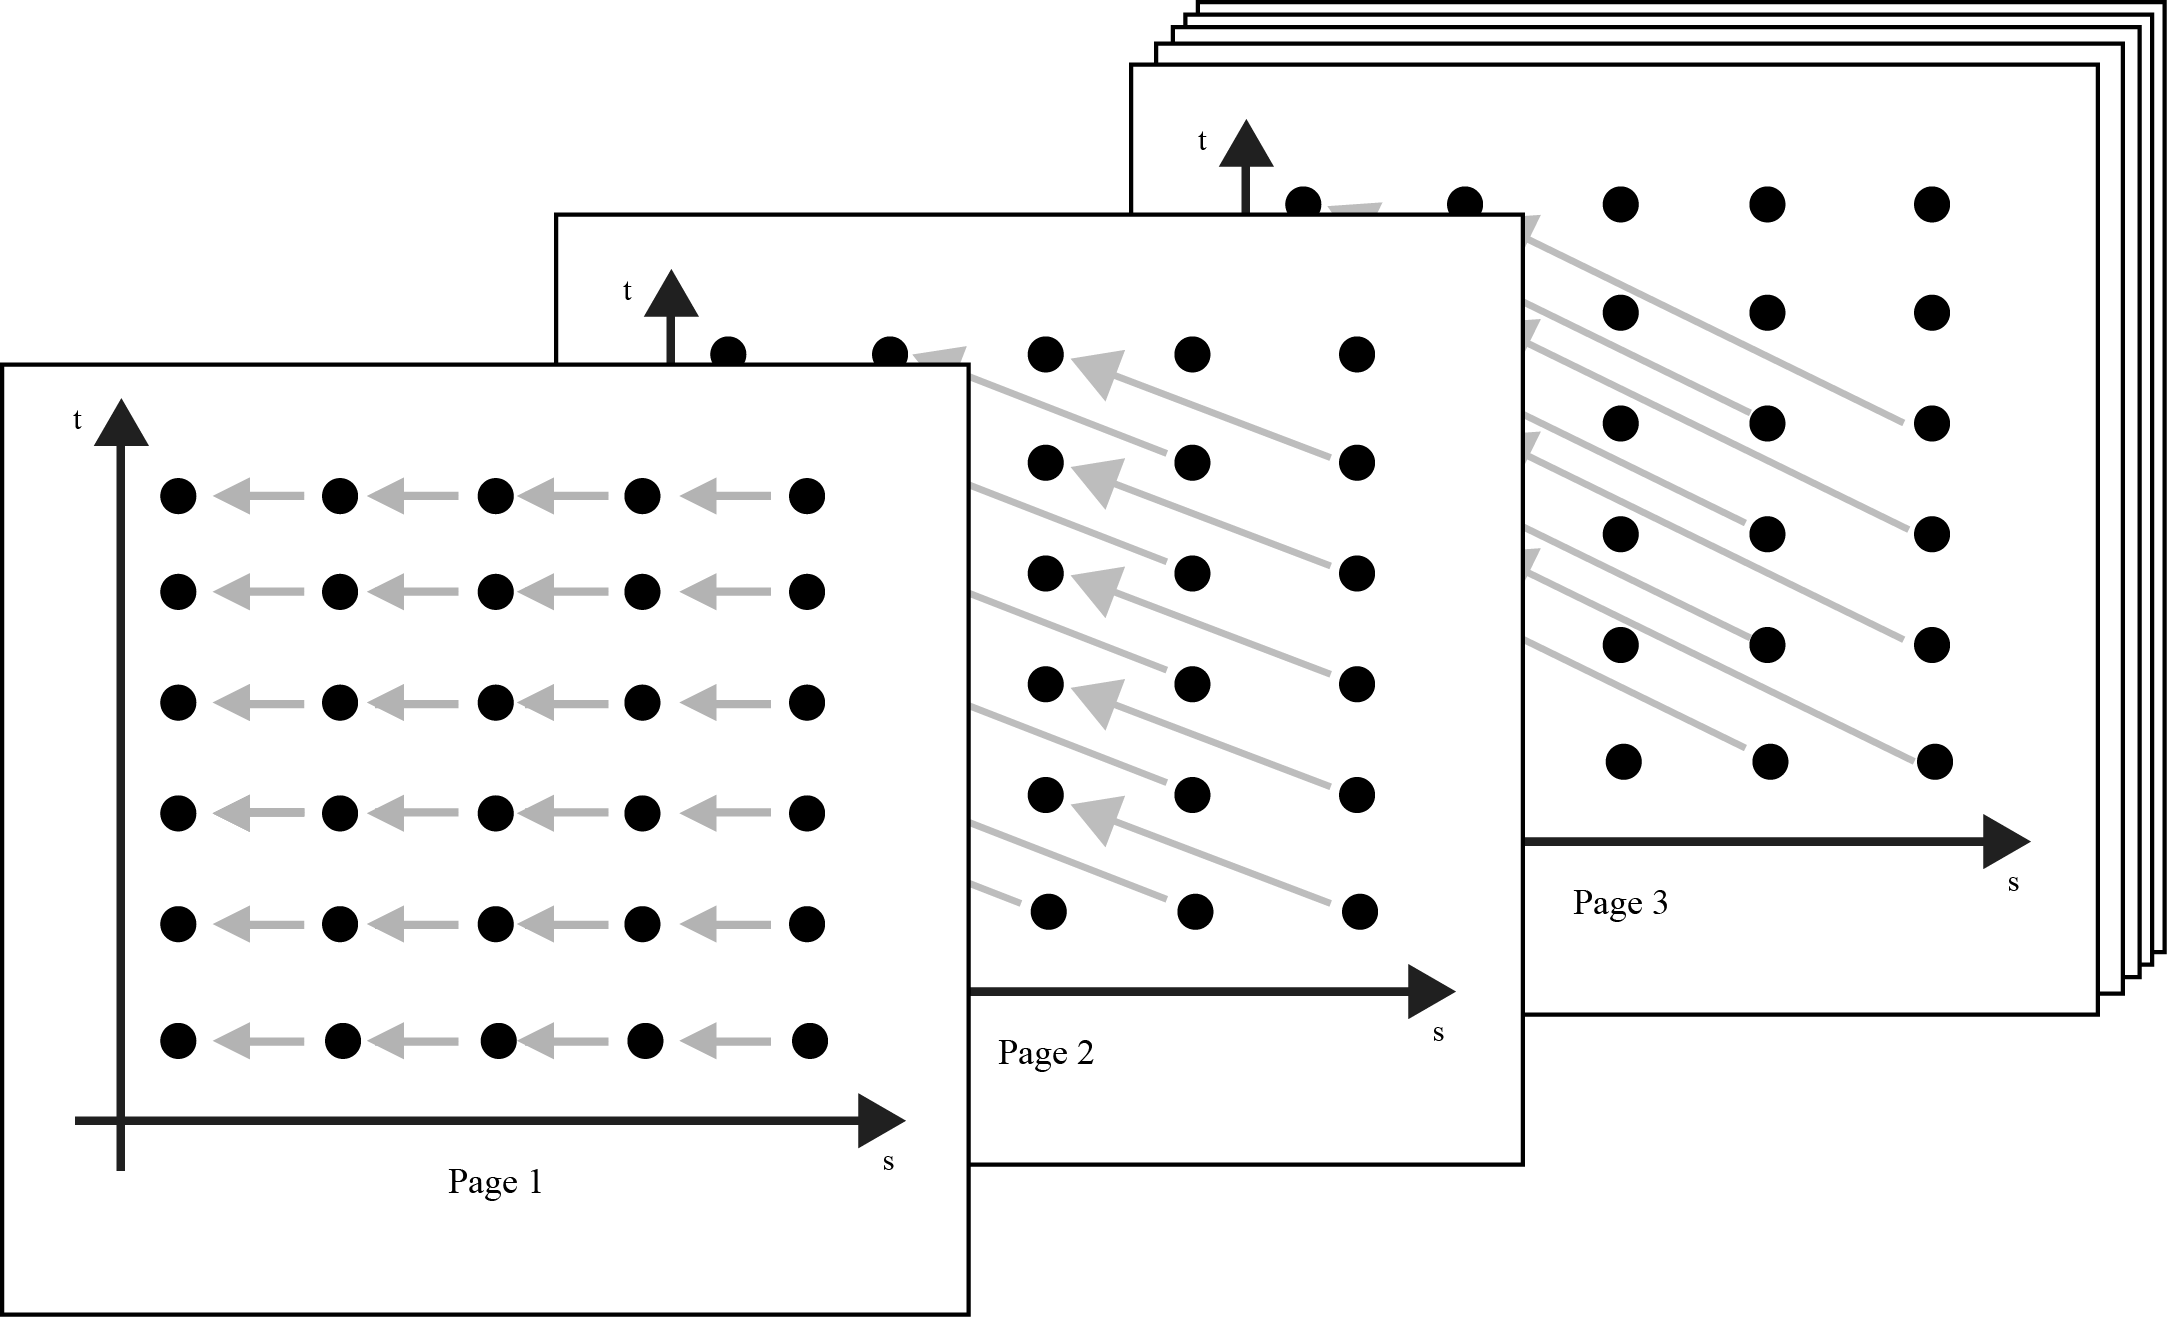
\includegraphics[width=\linewidth,height=0.45\textheight,keepaspectratio]{figures/cover.png}
  \end{center}
       \begin{minipage}{.35\linewidth}
    \begin{flushleft}
      \vspace{2em}
      {\fontsize{6pt}{2pt} \textit{Notes: These are notes live-tex'd
from a graduate course in Homological Algebra taught by Brian Boe at the
University of Georgia in Spring 2021. As such, any errors or
inaccuracies are almost certainly my own. } } \\
    \end{flushleft}
    \end{minipage}
    \hfill
    \begin{minipage}{.65\linewidth}
    \end{minipage}
  }







\begin{document}

\date{}
\author{D. Zack Garza}
\maketitle
\begin{flushleft}
\textit{D. Zack Garza} \\
\textit{University of Georgia} \\
  \textit{\href{mailto: dzackgarza@gmail.com}{dzackgarza@gmail.com}} \\
{\tiny \textit{Last updated:} 2021-04-22 }
\end{flushleft}


\newpage

% Note: addsec only in KomaScript
\addsec{Table of Contents}
\tableofcontents
\newpage

\hypertarget{wednesday-january-13}{%
\section{Wednesday, January 13}\label{wednesday-january-13}}

Reference:

\begin{itemize}
\item
  The course text is Weibel \autocite{weibel_2011}.
\item
  See the many corrections/errata:
  \url{http://www.math.rutgers.edu/~weibel/Hbook-corrections.html}
\item
  Sections we'll cover:

  \begin{itemize}
  \tightlist
  \item
    1.1-1.5,
  \item
    2.2-2.7,
  \item
    3.4,
  \item
    3.6,
  \item
    6.1,
  \item
    5.1-5.2,
  \item
    5.4-5.8,
  \item
    6.8,
  \item
    6.7,
  \item
    6.3,
  \item
    7.1-7.5,
  \item
    7.7-7.8,
  \item
    Appendix A (when needed)
  \end{itemize}
\item
  Course Website:
  \url{https://uga.view.usg.edu/d2l/le/content/2218619/viewContent/33763436/View}
\end{itemize}

\hypertarget{overview}{%
\subsection{Overview}\label{overview}}

\begin{definition}[Exact complexes]

A \textbf{complex} is given by
\begin{align*}
\cdots \xrightarrow{d_{i-1}} M_{i-1} \xrightarrow{d_i} M_i \xrightarrow{d_{i+1}}M_{i+1} \to  \cdots
.\end{align*}
where \(M_i \in {\mathsf{R}{\hbox{-}}\mathsf{Mod}}\) and
\(d_i \circ d_{i-1} = 0\), which happens if and only if
\(\operatorname{im}d_{i-1} \subseteq \ker d_i\). If
\(\operatorname{im}d_{i-1} = \ker d_i\), this complex is \textbf{exact}.

\end{definition}

\begin{example}[?]

We can apply a functor such as \(\otimes_R N\) to get a new complex
\begin{align*}
\cdots \xrightarrow{d_{i-1} \otimes 1_N} M_{i-1} \otimes_R N \xrightarrow{d_i \otimes 1} M_i \otimes N  \to M_{i+1} \xrightarrow{d_{i+1} \otimes 1} \cdots
.\end{align*}

\end{example}

\begin{example}[?]

Applying \(\mathop{\mathrm{Hom}}(N, {-})\) similarly yields
\begin{align*}
\mathop{\mathrm{Hom}}_R(N, M_{i}) \xrightarrow{d_{i-1}^*} \mathop{\mathrm{Hom}}_R(N, M_{i+1})
,\end{align*}
where \(d_i^* = d_i \circ ({-})\) is given by composition.

\end{example}

\begin{example}[?]

Applying \(\mathop{\mathrm{Hom}}({-}, N)\) yields
\begin{align*}
\mathop{\mathrm{Hom}}_R(M_i, N) \xrightarrow{d_{i}^*} \mathop{\mathrm{Hom}}_R(M_{i+1}, N)
\end{align*}
where \(d_i^* = ({-}) \circ d_i\).

\end{example}

\begin{remark}

Note that we can also take complexes with arrows in the other direction.
For \(F\) a functor, we can rewrite these examples as
\begin{align*}
d_i^* \circ d_{i-1}^* = F(d_i) \circ F(d_{i-1}) = F(d_i \circ d_{i-1}) = F(0) = 0
,\end{align*}
provided \(F\) is nice enough and sends zero to zero. This follows from
the fact that functors preserve composition. Even if the original
complex is exact, the new one may not be, so we can define the
following:

\end{remark}

\begin{definition}[Cohomology]

\begin{align*}
H^i(M^*) = \ker d_i^* / \operatorname{im}d_{i-1}^*
.\end{align*}

\end{definition}

\begin{remark}

These will lead to \textbf{\(i\)th derived functors}, and category
theory will be useful here. See appendix in Weibel. For a category
\(\mathcal{C}\) we'll define

\begin{itemize}
\tightlist
\item
  \(\mathrm{Obj}(\mathcal{C} )\) as the objects
\item
  \(\mathop{\mathrm{Hom}}_{\mathcal{C}}(A, B)\) a set of morphisms
  between them, where a more modern notation might be
  \(\mathrm{Mor}(A, B)\).
\item
  Morphisms compose: \(A \xrightarrow{f} B \xrightarrow{g} C\) means
  that \(g\circ f \in \mathop{\mathrm{Hom}}_{\mathcal{C}}(A, C)\)
\item
  Associativity
\item
  Identity morphisms
\end{itemize}

See the appendix for diagrams defining zero objects and the zero map,
which we'll need to make sense of exactness. We'll also needs notions of
kernels and images, or potentially cokernels instead of images since
they're closely related.

\end{remark}

\begin{remark}

In the examples, we had \(\ker d_i \subseteq M_i\), but this need not be
true since the objects in the category may not be sets. Such an example
is the category of complexes of \(R{\hbox{-}}\)modules:
\(\operatorname{Cx}({\mathsf{R}{\hbox{-}}\mathsf{Mod}})\). In this
setting, kernels will be subcomplexes but not subsets.

\end{remark}

\begin{definition}[Functors]

Recall that \textbf{functors} are ``functions'' between categories
\(F: \mathcal{C}\to \mathcal{D}\) such that

\begin{itemize}
\item
  Objects are sent to objects,
\item
  Morphisms are sent to morphisms, so
  \(A \xrightarrow{f} B \leadsto F(A) \xrightarrow{F(f)} F(B)\),
\item
  \(F\) respects composition and identities
\end{itemize}

\end{definition}

\begin{example}[Hom]

\(\mathop{\mathrm{Hom}}_R(N, {-}): {\mathsf{R}{\hbox{-}}\mathsf{Mod}}\to {\mathsf{Ab}}\),
noting that the hom set may not have an \(R{\hbox{-}}\)module structure.

\end{example}

\begin{remark}

Taking cohomology yields the \(i\)th derived functors of \(F\), for
example \(\operatorname{Ext}^i, \operatorname{Tor}_i\). Recall that
functors can be \emph{covariant} or contravariant. See section 1 for
formulating simplicial and singular homology (from topology) in this
language.

\end{remark}

\hypertarget{chapter-1-chain-complexes}{%
\subsection{Chapter 1: Chain
Complexes}\label{chapter-1-chain-complexes}}

\hypertarget{complexes-of-rhbox-modules}{%
\subsubsection{\texorpdfstring{Complexes of
\(R{\hbox{-}}\)modules}{Complexes of R\{\textbackslash hbox\{-\}\}modules}}\label{complexes-of-rhbox-modules}}

\begin{definition}[Exactness]

Let \(R\) be a ring with 1 and define
\({\mathsf{R}{\hbox{-}}\mathsf{Mod}}\) to be the category of
\emph{right} \(R{\hbox{-}}\)modules.
\(A \xrightarrow{f} B \xrightarrow{g} C\) is \textbf{exact} if and only
if \(\ker g = \operatorname{im}f\), and in particular \(g\circ f = 0\).

\end{definition}

\begin{definition}[Chain Complex]

A \textbf{chain complex} is
\begin{align*}
C_{-}\coloneqq(C_{-}, d_{-}) \coloneqq\qty{ \cdots \to C_{n+1} \xrightarrow{d_{n+1}} C_n \xrightarrow{d_n} C_{n-1} \to \cdots }
\end{align*}
for \(n \in {\mathbb{Z}}\) such that \(d_n \circ d_{n+1} = 0\). We drop
the \(n\) from the notation and write \(d^2 \coloneqq d\circ d = 0\).

\end{definition}

\begin{definition}[Cycles and boundaries]

\envlist

\begin{itemize}
\tightlist
\item
  \(Z_n = Z_n(C_{-}) = \ker d_n\) are referred to as
  \textbf{\(n{\hbox{-}}\)cycles}.
\item
  \(B_n = B_n(C_{-}) = \operatorname{im}d_{n+1}\) are the
  \textbf{\(n{\hbox{-}}\)boundaries}.
\end{itemize}

\end{definition}

\begin{definition}[Homology of a chain complex]

Note that if \(d^2 = 0\) then \(B_n \leq Z_n \leq C_n\). In this case,
it makes sense to define the quotient module
\(H^n(C_{-}) \coloneqq Z_n / B_n\), the \textbf{\(n\)th homology} of
\(C_{-}\).

\end{definition}

\begin{definition}[Maps of chain complexes]

A map \(u: C_{-}\to D_{-}\) of chain complexes is a sequence of maps
\(u_n: C_n \to D_n\) such that all of the following squares commute:

\begin{center}
\begin{tikzcd}
    {\cdots} & {C_{n+1}} & {C_n} & {C_{n-1}} & {\cdots} \\
    \\
    {\cdots} & {D_{n+1}} & {D_n} & {D_{n-1}} & {\cdots}
    \arrow[from=1-1, to=1-2]
    \arrow[from=1-2, to=1-3]
    \arrow[from=1-3, to=1-4]
    \arrow[from=3-1, to=3-2]
    \arrow[from=3-2, to=3-3]
    \arrow[from=3-3, to=3-4]
    \arrow[from=3-4, to=3-5]
    \arrow[from=1-4, to=1-5]
    \arrow["{u_{n+1}}", from=1-2, to=3-2]
    \arrow["{u_n}", from=1-3, to=3-3]
    \arrow["{u_{n-1}}", from=1-4, to=3-4]
\end{tikzcd}
\end{center}

\begin{quote}
\href{https://q.uiver.app/?q=WzAsMTAsWzEsMCwiQ197bisxfSJdLFsyLDAsIkNfbiJdLFszLDAsIkNfe24tMX0iXSxbMSwyLCJEX3tuKzF9Il0sWzIsMiwiRF9uIl0sWzMsMiwiRF97bi0xfSJdLFswLDAsIlxcYnVsbGV0Il0sWzAsMiwiXFxidWxsZXQiXSxbNCwyLCJcXGJ1bGxldCJdLFs0LDAsIlxcYnVsbGV0Il0sWzYsMF0sWzAsMV0sWzEsMl0sWzcsM10sWzMsNF0sWzQsNV0sWzUsOF0sWzIsOV0sWzAsMywidV97bisxfSIsMV0sWzEsNCwidV9uIiwxXSxbMiw1LCJ1X3tuLTF9IiwxXV0=}{Link
to Diagram}
\end{quote}

\end{definition}

\begin{remark}

We can thus define a category
\(\mathrm{Ch}({\mathsf{R}{\hbox{-}}\mathsf{Mod}})\) where

\begin{itemize}
\tightlist
\item
  The objects are chain complexes,
\item
  The morphisms are chain maps.
\end{itemize}

\end{remark}

\begin{exercise}[Weibel 1.1.2]

A chain complex map \(u: C_{-}\to D_{-}\) restricts to
\begin{align*}
u_n: Z_n(C_{-}) \to Z_n(D_{-}) \\
u_n: B_n(D_{-}) \to B_n(D_{-})
\end{align*}
and thus induces a well-defined map
\(u_{n, *}: H_n(C_{-}) \to H_n(D_{-})\).

\end{exercise}

\begin{remark}

Each \(H_n\) thus becomes a functor
\(\mathrm{Ch}({\mathsf{R}{\hbox{-}}\mathsf{Mod}}) \to {\mathsf{R}{\hbox{-}}\mathsf{Mod}}\)
where \(H_n(u) \coloneqq u_{*. n}\).

\end{remark}

\hypertarget{friday-january-15}{%
\section{Friday, January 15}\label{friday-january-15}}

\hypertarget{review}{%
\subsection{Review}\label{review}}

\begin{quote}
See assignment posted on ELC, due Wed Jan 27
\end{quote}

\begin{remark}

Recall that a chain complex is \(C_{-}\) where \(d^2 = 0\), and a map of
chain complex is a ladder of commuting squares

\begin{center}
\begin{tikzcd}
    \cdots & {C_{n-1}} & {C_{n}} & {C_{n+1}} & \cdots \\
    && {} \\
    \cdots & {D_{n-1}} & {D_n} & {D_{n+1}} & \cdots
    \arrow["{u_{n-1}}", from=1-2, to=3-2]
    \arrow["{u_n}", from=1-3, to=3-3]
    \arrow["{u_{n+1}}", from=1-4, to=3-4]
    \arrow["{d_{n-1}}", from=1-2, to=1-3]
    \arrow["{d_n}", from=1-3, to=1-4]
    \arrow["{d_{n-1}}", from=3-2, to=3-3]
    \arrow["{d_n}"', from=3-3, to=3-4]
    \arrow[from=1-4, to=1-5]
    \arrow[from=3-4, to=3-5]
    \arrow[from=3-1, to=3-2]
    \arrow[from=1-1, to=1-2]
\end{tikzcd}
\end{center}

\begin{quote}
\href{https://q.uiver.app/?q=WzAsMTEsWzEsMCwiQ197bi0xfSJdLFsyLDAsIkNfe259Il0sWzMsMCwiQ197bisxfSJdLFsyLDIsIkRfbiJdLFszLDIsIkRfe24rMX0iXSxbMSwyLCJEX3tuLTF9Il0sWzQsMCwiXFxidWxsZXQiXSxbNCwyLCJcXGJ1bGxldCJdLFswLDIsIlxcYnVsbGV0Il0sWzAsMCwiXFxidWxsZXQiXSxbMiwxXSxbMCw1LCJ1Il0sWzEsMywidV9uIl0sWzIsNCwidSJdLFswLDFdLFsxLDIsImRfbiJdLFs1LDNdLFszLDQsImRfbiIsMl0sWzIsNl0sWzQsN10sWzgsNV0sWzksMF1d}{Link
to diagram}
\end{quote}

Recall that \(u_n: Z_n(C) \to Z_n(D)\) and \(u_n: B_n(C) \to B_n(D)\)
preserves these submodules, so there are induced maps
\(u_{{-}, n}: H_n(D) \to H_n(D)\) where
\(H_n(C) \coloneqq Z_n(C) / B_nn-1(C)\). Moreover, taking \(H_n({-})\)
is a functor from
\(\mathsf{Ch}({\mathsf{R}{\hbox{-}}\mathsf{Mod}}) \to {\mathsf{R}{\hbox{-}}\mathsf{Mod}}\)
for any fixed \(n\) and on objects \(C\mapsto H_n(C)\) and chain maps
\(u_{n} \to H_n(u) \coloneqq u_{*, n}\). Note the lower indices denote
maps going down in degree.

\end{remark}

\hypertarget{cohomology}{%
\subsection{Cohomology}\label{cohomology}}

\begin{definition}[Quasi-isomorphism]

A chain map \(u:C\to D\) is a \textbf{quasi-isomorphism} if and only if
the induced map \(u_{*, n}: H^n(C) \to H^n(D)\) is an isomorphism of
\(R{\hbox{-}}\)modules.

\end{definition}

\begin{remark}

Note that the usual notion of an isomorphism in the categorical sense
might be too strong here.

\end{remark}

\begin{definition}[Cohomology]

A \textbf{cochain complex} is a complex of the form
\begin{align*}
\cdots 
\xrightarrow{d^{n-2}}  C^{n-1}
\xrightarrow{d^{n-1}}  C^{n}
\xrightarrow{d^{n}}  C^{n+1}
\cdots
\end{align*}
where \(d^n \circ d^{n-1} = 0\). We similarly write
\(Z^n(C) \coloneqq\ker d^n\) and
\(B^n(C) \coloneqq\operatorname{im}d^{n-1}\) and write the
\(R{\hbox{-}}\)module \(H^n(C) \coloneqq Z^n/B^n\) for the \(n\)th
\textbf{cohomology} of \(C\).

\end{definition}

\begin{remark}

There is a way to go back and forth bw chain complexes and cochain
complexes: set \(C_n \coloneqq C^{-n}\) and \(d_n \coloneqq d^{-n}\).
This yields
\begin{align*}
C^{-n} 
\xrightarrow{d^{-n}} 
C^{-n+1} 
\iff C_n \xrightarrow{d^n} C_{n-1}
,\end{align*}
and the notions of \(d^2 = 0\) coincide.

\end{remark}

\begin{definition}[Bounded complexes]

A cochain complex \(C\) is \textbf{bounded} if and only if there exists
an \(a\leq b \in {\mathbb{Z}}\) such that
\(C_n \neq 0 \iff a\leq n \leq b\). Similarly \(C^n\) is bounded above
if there is just a \(b\), and \textbf{bounded below} for just an \(a\).
All of the same definitions are made for cochain complexes.

\end{definition}

\begin{remark}

See the book for classical applications:

\begin{itemize}
\tightlist
\item
  1.1.3: Simplicial homology
\item
  1.1.5: Singular homology
\end{itemize}

\end{remark}

\hypertarget{operations-on-chain-complexes}{%
\subsection{Operations on Chain
Complexes}\label{operations-on-chain-complexes}}

\begin{remark}

Write \(\mathsf{Ch}\) for
\(\mathsf{Ch}({\mathsf{R}{\hbox{-}}\mathsf{Mod}})\), then if
\(f,g: C\to D\) are chain maps then \(f+g:C\to D\) can be defined as
\((f+g)(x) = f(x) + g(x)\), since \(D\) has an addition coming from its
\(R{\hbox{-}}\)module structure. Thus the hom sets
\(\mathop{\mathrm{Hom}}_{\mathsf{Ch}}(C, D)\) becomes an abelian group.
There is a distinguished \textbf{zero object}\footnote{See appendix A
  1.6 for initial and terminal objects. Note that \(\emptyset\) is an
  initial but non-terminal object in \({\mathsf{Set}}\), whereas zero
  objects are both.} \(0\), defined as the chain complex with all zero
objects and all zero maps. Note that we also have a zero map given by
the composition \((C \to 0) \circ (0\to D)\).

\end{remark}

\begin{definition}[Products and Coproducts]

If \(\left\{{A_ \alpha}\right\}\) is a family of complexes, we can form
two new complexes:

\begin{itemize}
\item
  The \textbf{product}
  \(\qty{ \prod_ \alpha A_ \alpha}_n \coloneqq\prod_ \alpha A _{\alpha, n}\)
  with the differential
  \begin{align*}
  \qty{ \prod d_ \alpha}_n: \prod A _{\alpha, n} \xrightarrow{d _{\alpha, n}} \prod A _{\alpha, n-1}
  .\end{align*}
\item
  The \textbf{coproduct}
  \(\qty{ \coprod _{\alpha} A _{\alpha}}_n \coloneqq\bigoplus _{\alpha} A _{\alpha, n}\),
  i.e.~there are only finitely many nonzero entries, with exactly the
  same definition as above for the differential.
\end{itemize}

\end{definition}

\begin{remark}

Note that if the index set is finite, these notions coincide. By
convention, finite direct products are written as direct sums.

These structures make \(\mathsf{Ch}\) into an \textbf{additive
category}. See appendix for definition: the homs are abelian groups
where composition distributes over addition, existence of a zero object,
and existence of finite products. Note that here we have arbitrary
products.

\end{remark}

\begin{definition}[Subcomplexes]

We say \(B\) is a \textbf{subcomplex} of \(C\) if and only if

\begin{itemize}
\tightlist
\item
  \(B_n \leq C_n \in {\mathsf{R}{\hbox{-}}\mathsf{Mod}}\) for all \(n\),
\item
  The differentials of \(B_n\) are the restrictions of the differentials
  of \(C_n\).
\end{itemize}

\end{definition}

\begin{remark}

This can be alternatively stated as saying the inclusion \(i: B\to C\)
given by \(i_n: B_n \to C_n\) is a morphism of chain complexes. Recall
that some squares need to commute, and this forces the condition on
restrictions.

\end{remark}

\begin{definition}[Quotient Complexes]

When \(B \leq C\), we can form the quotient complex \(C/B\) where
\begin{align*}
C_n/B_n \xrightarrow{\mkern 1.5mu\overline{\mkern-1.5mud_n\mkern-1.5mu}\mkern 1.5mu} C _{n-1} / B _{n-1}
.\end{align*}
Moreover there is a natural projection \(\pi: C\to C/B\) which is a
chain map.

\end{definition}

\begin{remark}

Suppose \(f:B\to C\) is a chain map, then there exist induced maps on
the levelwise kernels and cokernels, so we can form the \textbf{kernel}
and \textbf{cokernel} complex:

\begin{center}
\begin{tikzcd}
    \cdots && {\ker f_n} && {\ker f_{n-1}} && \cdots \\
    \\
    \cdots && {B_n} && {B_{n-1}} && \cdots \\
    \\
    \cdots && {C_n} && {C_{n-1}} && \cdots \\
    &&& {} & {} \\
    \cdots && {\operatorname{coker}f_n} && {\operatorname{coker}f_{n-1}} && \cdots
    \arrow["{d_n}", from=5-3, to=5-5]
    \arrow["{d_n}", from=3-3, to=3-5]
    \arrow["{\exists d_n}", dashed, from=1-3, to=1-5]
    \arrow["{\exists d_n}", dashed, from=7-3, to=7-5]
    \arrow["{i_{n}}"{description}, from=1-3, to=3-3]
    \arrow["{f_n}"{description}, from=3-3, to=5-3]
    \arrow["{\pi_n}"{description}, from=5-3, to=7-3]
    \arrow["{f_{n-1}}"{description}, from=3-5, to=5-5]
    \arrow["{\pi_{n-1}}"{description}, from=5-5, to=7-5]
    \arrow["{i_{n-1}}"{description}, from=1-5, to=3-5]
    \arrow[from=1-1, to=1-3]
    \arrow[from=3-1, to=3-3]
    \arrow[from=5-1, to=5-3]
    \arrow[from=7-1, to=7-3]
    \arrow[from=7-5, to=7-7]
    \arrow[from=5-5, to=5-7]
    \arrow[from=3-5, to=3-7]
    \arrow[from=1-5, to=1-7]
\end{tikzcd}
\end{center}

\begin{quote}
\href{https://q.uiver.app/?q=WzAsMTgsWzIsNCwiQ19uIl0sWzQsNCwiQ197bi0xfSJdLFsyLDIsIkJfbiJdLFs0LDIsIkJfe24tMX0iXSxbMiwwLCJcXGtlciBmX24iXSxbNCwwLCJcXGtlciBmX3tuLTF9Il0sWzIsNiwiXFxjb2sgZl9uIl0sWzQsNiwiXFxjb2sgZl97bi0xfSJdLFszLDVdLFs0LDVdLFs2LDAsIlxcY2RvdHMiXSxbNiwyLCJcXGNkb3RzIl0sWzYsNCwiXFxjZG90cyJdLFs2LDYsIlxcY2RvdHMiXSxbMCw2LCJcXGNkb3RzIl0sWzAsNCwiXFxjZG90cyJdLFswLDIsIlxcY2RvdHMiXSxbMCwwLCJcXGNkb3RzIl0sWzAsMSwiZF9uIl0sWzIsMywiZF9uIl0sWzQsNSwiXFxleGlzdHMgZF9uIiwwLHsic3R5bGUiOnsiYm9keSI6eyJuYW1lIjoiZGFzaGVkIn19fV0sWzYsNywiXFxleGlzdHMgZF9uIiwwLHsic3R5bGUiOnsiYm9keSI6eyJuYW1lIjoiZGFzaGVkIn19fV0sWzQsMiwiaV97bn0iLDFdLFsyLDAsImZfbiIsMV0sWzAsNiwiXFxwaV9uIiwxXSxbMywxLCJmX3tuLTF9IiwxXSxbMSw3LCJcXHBpX3tuLTF9IiwxXSxbNSwzLCJpX3tuLTF9IiwxXSxbMTcsNF0sWzE2LDJdLFsxNSwwXSxbMTQsNl0sWzcsMTNdLFsxLDEyXSxbMywxMV0sWzUsMTBdXQ==}{Link
to Diagram}
\end{quote}

Here \(\ker f \leq B\) is a subcomplex, and \(\operatorname{coker}f\) is
a quotient complex of \(C\). The chain map \(i: \ker f\to B\) is a
categorical kernel of \(f\) in \(\mathsf{Ch}\), and \(\pi\) is similarly
a cokernel. See appendix A 1.6. These constructions make \(\mathsf{Ch}\)
into an \textbf{abelian category}: roughly an additive category where
every morphism has a kernel and a cokernel.

\end{remark}

\hypertarget{chain-complex-of-chain-complexes-wednesday-january-20}{%
\section{1.2: Chain Complex of Chain Complexes (Wednesday, January
20)}\label{chain-complex-of-chain-complexes-wednesday-january-20}}

\begin{quote}
See phone pic for missed first 10m
\end{quote}

\hypertarget{double-complexes}{%
\subsection{Double Complexes}\label{double-complexes}}

\begin{remark}

Consider a double complex:

\begin{center}
\begin{tikzcd}
    &&&&&& {C_{p, \cdot}:} \\
    &&&& \vdots && \vdots && \vdots \\
    \\
    && \cdots && {C_{p-1, q+1}} && {C_{p, q+1}} && {C_{p+1, q+1}} && \cdots \\
    \\
    {C_{\cdot, q}:} && \cdots && {C_{p-1, q}} && {C_{p, q}} && {C_{p+1, q}} && \cdots \\
    \\
    && \cdots && {C_{p-1, q+1}} && {C_{p, q+1}} && {C_{p+1, q+1}} && \cdots \\
    \\
    &&&& \vdots && \vdots && \vdots
    \arrow["{d_{p, q}^h}", from=6-7, to=6-5]
    \arrow["{d_{p, q}^v}", from=6-7, to=8-7]
    \arrow["{d_{p, q+1}^v}", from=4-7, to=6-7]
    \arrow["{d_{p+1, q+1}^v}", from=4-9, to=6-9]
    \arrow["{d_{p+1, q}^v}", from=6-9, to=8-9]
    \arrow["{d_{p-1, q}^v}", from=6-5, to=8-5]
    \arrow["{d_{p-1, q+1}^v}", from=4-5, to=6-5]
    \arrow[from=8-5, to=10-5]
    \arrow[from=8-7, to=10-7]
    \arrow[from=8-9, to=10-9]
    \arrow["{d_{p+1, q+1}^h}", from=8-9, to=8-7]
    \arrow["{d_{p+1, q}^h}", from=6-9, to=6-7]
    \arrow["{d_{p, q+1}^h}", from=8-7, to=8-5]
    \arrow["{d_{p+1, q+1}^h}"{description}, from=4-9, to=4-7]
    \arrow["{d_{p, q+1}^h}"{description}, from=4-7, to=4-5]
    \arrow[from=2-5, to=4-5]
    \arrow[from=2-7, to=4-7]
    \arrow[from=2-9, to=4-9]
    \arrow[from=4-5, to=4-3]
    \arrow[from=6-5, to=6-3]
    \arrow[from=8-5, to=8-3]
    \arrow[from=8-11, to=8-9]
    \arrow[from=6-11, to=6-9]
    \arrow[from=4-11, to=4-9]
\end{tikzcd}
\end{center}

\begin{quote}
\href{https://q.uiver.app/?q=WzAsMjMsWzQsMywiQ197cC0xLCBxKzF9Il0sWzYsMywiQ197cCwgcSsxfSJdLFs4LDMsIkNfe3ArMSwgcSsxfSJdLFs0LDUsIkNfe3AtMSwgcX0iXSxbNiw1LCJDX3twLCBxfSJdLFs4LDUsIkNfe3ArMSwgcX0iXSxbNCw3LCJDX3twLTEsIHErMX0iXSxbNiw3LCJDX3twLCBxKzF9Il0sWzgsNywiQ197cCsxLCBxKzF9Il0sWzYsMSwiXFx2ZG90cyJdLFsyLDUsIlxcY2RvdHMiXSxbNCw5LCJcXHZkb3RzIl0sWzYsOSwiXFx2ZG90cyJdLFs4LDksIlxcdmRvdHMiXSxbMCw1LCJDX3tcXGNkb3QsIHF9OiJdLFsyLDcsIlxcY2RvdHMiXSxbMTAsNywiXFxjZG90cyJdLFsxMCw1LCJcXGNkb3RzIl0sWzEwLDMsIlxcY2RvdHMiXSxbMiwzLCJcXGNkb3RzIl0sWzYsMCwiQ197cCwgXFxjZG90fToiXSxbNCwxLCJcXHZkb3RzIl0sWzgsMSwiXFx2ZG90cyJdLFs0LDMsImRfe3AsIHF9XmgiXSxbNCw3LCJkX3twLCBxfV52Il0sWzEsNCwiZF97cCwgcSsxfV52Il0sWzIsNSwiZF97cCsxLCBxKzF9XnYiXSxbNSw4LCJkX3twKzEsIHF9XnYiXSxbMyw2LCJkX3twLTEsIHF9XnYiXSxbMCwzLCJkX3twLTEsIHErMX1ediJdLFs2LDExXSxbNywxMl0sWzgsMTNdLFs4LDcsImRfe3ArMSwgcSsxfV5oIl0sWzUsNCwiZF97cCsxLCBxfV5oIl0sWzcsNiwiZF97cCwgcSsxfV5oIl0sWzIsMSwiZF97cCsxLCBxKzF9XmgiLDFdLFsxLDAsImRfe3AsIHErMX1eaCIsMV0sWzIxLDBdLFs5LDFdLFsyMiwyXSxbMCwxOV0sWzMsMTBdLFs2LDE1XSxbMTYsOF0sWzE3LDVdLFsxOCwyXV0=}{Link
to Diagram}
\end{quote}

All of the individual rows and columns are chain complexes, where
\((d^h)^2 = 0\) and \((d^v)^2 = 0\), and the square anticommute:
\(d^v d^h + d^h d^v - 0\), so \(d^v d^h = -d^h d^v\). This is almost a
chain complex of chain complexes, i.e.~an element of
\(\mathsf{Ch}(\mathsf{Ch}{\mathsf{R}{\hbox{-}}\mathsf{Mod}}))\). It's
useful here to consider lines parallel to the line \(y=x\).

\end{remark}

\begin{definition}[Bounded Complexes]

A double complex \(C_{{-}, {-}}\) is \textbf{bounded} if and only if
there are only finitely many nonzero terms along each constant diagonal
\(p+q = n\).

\end{definition}

\begin{example}[?]

A \emph{first quadrant} double complex
\(\left\{{C_{p, q}}\right\}_{p, q\geq 0}\) is bounded: note that this
can still have infinitely many terms, but each diagonal is finite
because each will hit a coordinate axis.

\end{example}

\begin{remark}[The sign trick]

The squares anticommute, since the \(d^v\) are not chain maps between
the horizontal chain complexes. This can be fixed by changing every one
out of four signs, defining
\begin{align*}
f_{*, q}: C_{*, q} \to C_{*, q-1} \\
f_{p, q} \coloneqq(-1)^p d^v_{p, q}: C_{p,q} \to C_{p, q-1}
.\end{align*}

This yields a new double complex where the signs of each column
alternate:

\begin{center}
\begin{tikzcd}
    {C_{0, q}} && {C_{1, q}} && {C_{2, q}} \\
    \\
    {C_{0, q-1}} && {C_{1, q-1}} && {C_{2, q-1}}
    \arrow["{d^v}", from=1-1, to=3-1]
    \arrow["{-d^v}", from=1-3, to=3-3]
    \arrow["{d^v}", from=1-5, to=3-5]
    \arrow["{d^h}"{description}, from=1-5, to=1-3]
    \arrow["{d^h}"{description}, from=1-3, to=1-1]
    \arrow["{d^h}"{description}, from=3-5, to=3-3]
    \arrow["{d^h}"{description}, from=3-3, to=3-1]
\end{tikzcd}
\end{center}

Now the squares commute and \(f_{{-}, q}\) are chain maps, so this
object is an element of
\(\mathsf{Ch}(\mathsf{Ch}{\mathsf{R}{\hbox{-}}\mathsf{Mod}})\).

\end{remark}

\hypertarget{total-complexes}{%
\subsection{Total Complexes}\label{total-complexes}}

\begin{remark}

Recall that products and coproducts of \(R{\hbox{-}}\)modules coincide
when the indexing set is finite.

\end{remark}

\begin{definition}[Total Complexes]

Given a double complex \(C_{{-}, {-}}\), there are two ordinary chain
complexes associated to it referred to as \textbf{total complexes}:
\begin{align*}
(\operatorname{Tot}^{\Pi}C)_n &\coloneqq\prod_{p+q = n} C_{p, q}\\
(\operatorname{Tot}^{\oplus}C)_n &\coloneqq\bigoplus_{p+q = n} C_{p, q}
.\end{align*}
Writing \(\operatorname{Tot}(C)\) usually refers to the former. The
differentials are given by
\begin{align*}
d_{p, q} = d^h + d^v: C_{p, q} \to C_{p-1, q} \oplus C_{p, q-1}
,\end{align*}
where \(C_{p, q} \subseteq \operatorname{Tot}^{\oplus}(C)_n\) and
\(C_{p-1, q} \oplus C_{p, q-1} \subseteq \operatorname{Tot}^{\oplus}(C)_{n-1}\).
Then you extend this to a differential on the entire diagonal by
defining \(d = \bigoplus_{p, q} d_{p, q}\).

\end{definition}

\begin{exercise}[?]

Check that \(d^2 = 0\), using \(d^v d^h + d^h d^v = 0\).

\end{exercise}

\begin{remark}

Some notes:

\begin{itemize}
\item
  \(\operatorname{Tot}^{\oplus}(C) = \operatorname{Tot}^{\Pi}(C)\) when
  \(C\) is bounded.
\item
  The total complexes need not exist if \(C\) is unbounded: one needs
  infinite direct products and infinite coproducts to exist in
  \(\mathcal{C}\). A category admitting these is called
  \textbf{complete} or \textbf{cocomplete}.\footnote{Recall that abelian
    categories are additive and only require \emph{finite}
    products/coproducts. A counterexample: categories of \emph{finite}
    abelian groups, where e.g.~you can't take infinite sums and stay
    within the category.}
\end{itemize}

\end{remark}

\hypertarget{more-operations}{%
\subsection{More Operations}\label{more-operations}}

\begin{definition}[Truncation below]

Fix \(n\in {\mathbb{Z}}\), and define the \textbf{\(n\)th truncation}
\(\tau_{\geq n}(C)\) by
\begin{align*}
\tau_{\geq n}(C) = 
\begin{cases}
0 & i < n  
\\
Z_n & i= n
\\
C_i & i > n .
\end{cases}
.\end{align*}

Pictorially:

\begin{center}
\begin{tikzcd}
    \cdots & 0 & {Z_n} & {C_{n+1}} & {C_{n+2}} & \cdots
    \arrow[from=1-2, to=1-1]
    \arrow["{d_n}"', from=1-3, to=1-2]
    \arrow["{d_{n+1}}"', from=1-4, to=1-3]
    \arrow["{d_{n+2}}"', from=1-5, to=1-4]
    \arrow[from=1-6, to=1-5]
\end{tikzcd}
\end{center}

\begin{quote}
\href{https://q.uiver.app/?q=WzAsNixbMCwwLCJcXGNkb3RzIl0sWzEsMCwiMCJdLFsyLDAsIlpfbiJdLFszLDAsIkNfe24rMX0iXSxbNCwwLCJDX3tuKzJ9Il0sWzUsMCwiXFxjZG90cyJdLFsxLDBdLFsyLDEsImRfbiIsMl0sWzMsMiwiZF97bisxfSIsMl0sWzQsMywiZF97bisyfSIsMl0sWzUsNF1d}{Link
to diagram}
\end{quote}

This is sometimes call the \textbf{good truncation of \(C\) below
\(n\)}.

\end{definition}

\begin{remark}

Note that
\begin{align*}
H_i(\tau_{\geq n} C) = 
\begin{cases}
0 & i < n  
\\
H_i(C) & i\geq n.
\end{cases}
.\end{align*}

\end{remark}

\begin{definition}[Truncation above]

We define the quotient complex
\begin{align*}
\tau_{<n} C \coloneqq C / \tau_{\geq n} C
.\end{align*}
which is \(C_i\) below \(n\), \(C_n/Z_n\) at \(n\). Thus is has homology
\begin{align*}
\begin{cases}
H_i(C) & i< n.
\\
0 & i \geq n
\end{cases}
.\end{align*}

\end{definition}

\begin{definition}[Translation]

If \(C\) is a chain complex and \(p\in {\mathbb{Z}}\), define a new
complex \(C[p]\) by
\begin{align*}
C[p]_n \coloneqq C_{n+p}
.\end{align*}

\begin{center}
\begin{tikzcd}
    {\text{Degrees}} & {-p} && 0 && p \\
    \\
    C & {C_{-p}} & \cdots & {C_0} & \cdots & {C_{p}} \\
    {C[p]} & {C_0} & \cdots & {C_p} & \cdots & {C_{2p}}
    \arrow[dashed, from=3-4, to=4-2]
    \arrow[dashed, from=3-6, to=4-4]
\end{tikzcd}
\end{center}

\begin{quote}
\href{https://q.uiver.app/?q=WzAsMTYsWzAsMiwiQyJdLFswLDMsIkNbcF0iXSxbMywyLCJDXzAiXSxbMywwLCIwIl0sWzAsMCwiXFx0ZXh0e0RlZ3JlZXN9Il0sWzEsMCwiLXAiXSxbMSwyLCJDX3stcH0iXSxbMywzLCJDX3AiXSxbMSwzLCJDXzAiXSxbMiwyLCJcXGNkb3RzIl0sWzIsMywiXFxjZG90cyJdLFs0LDMsIlxcY2RvdHMiXSxbNCwyLCJcXGNkb3RzIl0sWzUsMiwiQ197cH0iXSxbNSwzLCJDX3sycH0iXSxbNSwwLCJwIl0sWzIsOCwiIiwwLHsic3R5bGUiOnsiYm9keSI6eyJuYW1lIjoiZGFzaGVkIn19fV0sWzEzLDcsIiIsMCx7InN0eWxlIjp7ImJvZHkiOnsibmFtZSI6ImRhc2hlZCJ9fX1dXQ==}{Link
to Diagram}
\end{quote}

Similarly, if \(C\) is a \emph{cochain} complex, we set
\(C[p]^n \coloneqq C^{n-p}\):

\begin{center}
\begin{tikzcd}
    {\text{Degrees}} & {-p} && 0 && p \\
    \\
    C & {C^{-p}} & \cdots & {C^0} & \cdots & {C^p} \\
    {C[p]} & {C^0} & \cdots & {C^{-p}} & \cdots & {C^0}
    \arrow[from=3-2, to=3-3]
    \arrow[from=3-3, to=3-4]
    \arrow[from=3-4, to=3-5]
    \arrow[from=3-5, to=3-6]
    \arrow[from=4-2, to=4-3]
    \arrow[from=4-3, to=4-4]
    \arrow[from=4-4, to=4-5]
    \arrow[from=4-5, to=4-6]
    \arrow[dashed, from=3-2, to=4-4]
    \arrow[dashed, from=3-4, to=4-6]
\end{tikzcd}
\end{center}

\begin{quote}
\href{https://q.uiver.app/?q=WzAsMTYsWzAsMiwiQyJdLFswLDMsIkNbcF0iXSxbMywyLCJDXjAiXSxbMywwLCIwIl0sWzAsMCwiXFx0ZXh0e0RlZ3JlZXN9Il0sWzEsMCwiLXAiXSxbMSwyLCJDXnstcH0iXSxbMywzLCJDXnstcH0iXSxbMSwzLCJDXjAiXSxbMiwyLCJcXGNkb3RzIl0sWzIsMywiXFxjZG90cyJdLFs0LDMsIlxcY2RvdHMiXSxbNCwyLCJcXGNkb3RzIl0sWzUsMiwiQ15wIl0sWzUsMywiQ14wIl0sWzUsMCwicCJdLFs2LDldLFs5LDJdLFsyLDEyXSxbMTIsMTNdLFs4LDEwXSxbMTAsN10sWzcsMTFdLFsxMSwxNF0sWzYsNywiIiwwLHsic3R5bGUiOnsiYm9keSI6eyJuYW1lIjoiZGFzaGVkIn19fV0sWzIsMTQsIiIsMCx7InN0eWxlIjp7ImJvZHkiOnsibmFtZSI6ImRhc2hlZCJ9fX1dXQ==}{Link
to Diagram}
\end{quote}

\begin{quote}
Mnemonic: Shift \(p\) positions in the same direction as the arrows.
\end{quote}

In both cases, the differentials are given by the shifted differential
\(d[p] \coloneqq(-1)^p d\). Note that these are not alternating: \(p\)
is the fixed translation, so this is a constant that changes the signs
of all differentials. Thus \(H_n(C[p]) = H_{n+p}(C)\) and
\(H^n(C[p]) = H^{n-p}\).

\end{definition}

\begin{exercise}

Check that if \(C^n \coloneqq C_{-n}\), then \(C[p]^n = C[p]_{-n}\).

\end{exercise}

\begin{remark}

We can make translation into a functor
\([p]: \mathsf{Ch}\to \mathsf{Ch}\): given \(f: C\to D\), define
\(f[p]: C[p] \to D[p]\) by \(f[p]_n \coloneqq f_{n+p}\), and a similar
definition for cochain complexes changing \(p\) to \(-p\).

\end{remark}

\hypertarget{lecture-4-friday-january-22}{%
\section{Lecture 4 (Friday, January
22)}\label{lecture-4-friday-january-22}}

\hypertarget{long-exact-sequences}{%
\subsection{Long Exact Sequences}\label{long-exact-sequences}}

\begin{remark}

Some terminology: in an abelian category \(\mathcal{A}\) an example of
an \textbf{exact complex} in \(\mathsf{Ch}(\mathcal{A})\) is
\begin{align*}
\cdots \to 0 \to A \xrightarrow{f} B \xrightarrow{g} C \to 0 \to \cdots
.\end{align*}

where \emph{exactness} means \(\ker = \operatorname{im}\) at each
position,
i.e.~\(\ker f = 0, \operatorname{im}f = \ker g, \operatorname{im}g = C\).
We say \(f\) is monic and \(g\) epic.

As a special case, if \(0\to A\to 0\) is exact then \(A\) must be zero,
since the image of the incoming map must be 0. This also happens when
every other term is zero. If \(0\to A \xrightarrow{f} B \to 0\), then
\(A \cong B\) since \(f\) is both injective and surjective (say for
\(R{\hbox{-}}\)modules).

\end{remark}

\begin{theorem}[Long Exact Sequences]

Suppose \(0\to A\to B \to C \to 0\) is a SES in
\(\mathsf{Ch}(\mathcal{A})\) (note: this is a sequence of
\emph{complexes}), then there are natural maps
\begin{align*}
\delta: H_n(C) \to H_{n-1}(A)
\end{align*}
called \textbf{connecting morphisms} which decrease degree such that the
following sequence is exact:

\begin{center}
\begin{tikzcd}
    & \cdots & {H_{n+1}(C)} \\
    \\
    {H_n(A)} & {H_n(B)} & {H_n(C)} \\
    \\
    {H_{n-1}(A)} & \cdots
    \arrow["{f_* = H_n(f)}", from=3-1, to=3-2]
    \arrow["{g_* = H_n(g)}", from=3-2, to=3-3]
    \arrow["\delta", from=1-3, to=3-1, in=180, out=360]
    \arrow["\delta", from=3-3, to=5-1, in=180, out=360]
    \arrow[from=5-1, to=5-2]
    \arrow[from=1-2, to=1-3]
\end{tikzcd}
\end{center}

\begin{quote}
\href{https://q.uiver.app/?q=WzAsNyxbMCwyLCJIX24oQSkiXSxbMSwyLCJIX24oQikiXSxbMiwyLCJIX24oQykiXSxbMiwwLCJIX3tuKzF9KEMpIl0sWzAsNCwiSF97bi0xfShBKSJdLFsxLDQsIlxcY2RvdHMiXSxbMSwwLCJcXGNkb3RzIl0sWzAsMSwiZl8qID0gSF9uKGYpIl0sWzEsMiwiZ18qID0gSF9uKGcpIl0sWzMsMCwiXFxkZWwiXSxbMiw0LCJcXGRlbCJdLFs0LDVdLFs2LDNdXQ==}{Link
to Diagram}
\end{quote}

This is referred to as the \textbf{long exact sequence in homology}.
Similarly, replacing chain complexes by cochain complexes yields a
similar connecting morphism that increases degree.

\begin{quote}
Note on notation: some books use \({{\partial}}\) for homology and
\(\delta\) for cohomology.
\end{quote}

\end{theorem}

The proof that this sequence exists is a consequence of the \emph{snake
lemma}.

\begin{lemma}[The Snake Lemma]

The sequence highlighted in red in the following diagram is exact:

\begin{center}
\begin{tikzcd}[column sep=tiny]
    0 && {{\color{red}\ker(f)}} && {{\color{red}\ker(\alpha)}} && {{\color{red}\ker(\beta)}} && {{\color{red}\ker(\gamma)}} \\
    \\
    && 0 && A && B && C && 0 \\
    &&&&&&& {} \\
    && 0 && {A'} && {B'} && {C'} && 0 \\
    \\
    &&&& {{\color{red}\operatorname{coker}(\alpha)}} && {{\color{red}\operatorname{coker}(\beta)}} && {{\color{red}\operatorname{coker}(\gamma)}} && {{\color{red}\operatorname{coker}(g')}} && 0
    \arrow[from=5-3, to=5-5]
    \arrow["{f'}"', from=5-5, to=5-7]
    \arrow["{g'}"', from=5-7, to=5-9]
    \arrow["f", from=3-5, to=3-7]
    \arrow["g", from=3-7, to=3-9]
    \arrow[from=3-3, to=3-5]
    \arrow["\beta"', from=3-7, to=5-7]
    \arrow["\gamma"', from=3-9, to=5-9]
    \arrow["\alpha"', from=3-5, to=5-5]
    \arrow[from=7-5, to=7-7]
    \arrow[from=7-7, to=7-9]
    \arrow[from=7-9, to=7-11]
    \arrow[from=7-11, to=7-13]
    \arrow[from=1-1, to=1-3]
    \arrow[from=1-3, to=1-5]
    \arrow[from=1-5, to=1-7]
    \arrow[from=1-7, to=1-9]
    \arrow[from=1-9, to=7-5, in=180, out=360, "\exists \delta", color=red, dotted]
    \arrow[from=5-9, to=5-11]
    \arrow[from=3-9, to=3-11]
    \arrow[from=1-5, to=3-5]
    \arrow[from=1-7, to=3-7]
    \arrow[from=1-9, to=3-9]
    \arrow[from=5-5, to=7-5]
    \arrow[from=5-7, to=7-7]
    \arrow[from=5-9, to=7-9]
\end{tikzcd}
\end{center}

\begin{quote}
\href{https://q.uiver.app/?q=WzAsMjEsWzQsMiwiQSJdLFs2LDIsIkIiXSxbOCwyLCJDIl0sWzQsNCwiQSciXSxbNiw0LCJCJyJdLFs4LDQsIkMnIl0sWzIsNCwiMCJdLFsyLDIsIjAiXSxbNCwwLCJ7XFxjb2xvcntyZWR9XFxrZXIoXFxhbHBoYSl9Il0sWzIsMCwie1xcY29sb3J7cmVkfVxca2VyKGYpfSJdLFs2LDAsIntcXGNvbG9ye3JlZH1cXGtlcihcXGJldGEpfSJdLFs4LDAsIntcXGNvbG9ye3JlZH1cXGtlcihcXGdhbW1hKX0iXSxbNCw2LCJ7XFxjb2xvcntyZWR9XFxjb2tlcihcXGFscGhhKX0iXSxbNiw2LCJ7XFxjb2xvcntyZWR9XFxjb2tlcihcXGJldGEpfSJdLFs4LDYsIntcXGNvbG9ye3JlZH1cXGNva2VyKFxcZ2FtbWEpfSJdLFsxMCw2LCJ7XFxjb2xvcntyZWR9XFxjb2tlcihnJyl9Il0sWzAsMCwiMCJdLFsxMiw2LCIwIl0sWzcsM10sWzEwLDIsIjAiXSxbMTAsNCwiMCJdLFs2LDNdLFszLDQsImYnIl0sWzQsNSwiZyciXSxbMCwxLCJmIl0sWzEsMiwiZyJdLFs3LDBdLFsxLDQsIlxcYmV0YSIsMV0sWzIsNSwiXFxnYW1tYSIsMV0sWzAsMywiXFxhbHBoYSIsMV0sWzEyLDEzXSxbMTMsMTRdLFsxNCwxNV0sWzE1LDE3XSxbMTYsOV0sWzksOF0sWzgsMTBdLFsxMCwxMV0sWzExLDEyXSxbNSwyMF0sWzIsMTldXQ==}{Link
to Diagram}
\end{quote}

\end{lemma}

\begin{proof}[of the Snake Lemma: Existence]

\envlist

\begin{itemize}
\tightlist
\item
  Start with \(c\in \ker(\gamma) \leq C\), so \(\gamma(c) = 0 \in C'\)
\item
  \textbf{Choose} \(b\in B\) by surjectivity

  \begin{itemize}
  \tightlist
  \item
    We'll show it's independent of this choice.
  \end{itemize}
\item
  Then \(b'\in B'\) goes to \(0\in C'\), so \(b' \in \ker (B' \to C')\)
\item
  By exactness,
  \(b' \in \ker (B' \to C') = \operatorname{im}(A'\to B')\), and now
  produce a unique \(a'\in A'\) by injectivity
\item
  Take the image \([a']\in \operatorname{coker}\alpha\)
\item
  Define \({{\partial}}(c) \coloneqq[a']\).
\end{itemize}

\end{proof}

\begin{proof}[of the Snake Lemma: Uniqueness]

\envlist

\begin{itemize}
\tightlist
\item
  We chose \(b\), suppose we chose a different \(\tilde b\).
\item
  Then \(\tilde b - b \mapsto c-c = 0\), so the difference is in
  \(\ker g = \operatorname{im}f\).
\item
  Produce an \(\tilde a\in A\) such that
  \(\tilde a\mapsto \tilde b - b\)
\item
  Then
  \(\mkern 1.5mu\overline{\mkern-1.5mua\mkern-1.5mu}\mkern 1.5mu \coloneqq\alpha(\tilde a)\),
  so apply \(f'\).
\item
  Define \(\beta(\tilde b) = \tilde b ' \in B\).
\item
  Commutativity of the LHS square forces
  \(\tilde a'\mapsto \tilde b' - b'\).
\item
  Then
  \(\mkern 1.5mu\overline{\mkern-1.5mua\mkern-1.5mu}\mkern 1.5mu + a' \mapsto \tilde b' -b' + b' = \tilde b'\).
\item
  So \(\tilde a' + a'\) is the desired pullback of \(\tilde b'\)
\item
  Then take \([\tilde a'] \in \operatorname{coker}\alpha\); are
  \(a', \tilde a'\) in the same equivalence class?
\item
  Use that fact that
  \(\tilde a = a' + \mkern 1.5mu\overline{\mkern-1.5mua\mkern-1.5mu}\mkern 1.5mu\),
  where
  \(\mkern 1.5mu\overline{\mkern-1.5mua\mkern-1.5mu}\mkern 1.5mu \in \operatorname{im}\alpha\),
  so
  \([\tilde a] = [a' + \mkern 1.5mu\overline{\mkern-1.5mua\mkern-1.5mu}\mkern 1.5mu] = [a'] \in \operatorname{coker}\alpha \coloneqq A'/\operatorname{im}\alpha\).
\end{itemize}

\end{proof}

\todo[inline]{A few changes in the middle, redo!}

\begin{proof}[of the Snake Lemma: Exactness]

\envlist

\begin{itemize}
\item
  Let's show \(g: \ker \beta\to \ker \gamma\).

  \begin{itemize}
  \tightlist
  \item
    Let \(b \in \ker \beta\), then consider
    \(\gamma(g(\beta)) = g'(\beta(b)) = g'(0) = 0\) and so
    \(g(b) \in \ker \gamma\).
  \end{itemize}
\item
  Now we'll show
  \(\operatorname{im}({ \left.{{g}} \right|_{{\ker \beta}} }) \subseteq \ker \delta\)

  \begin{itemize}
  \tightlist
  \item
    Let \(b \in \ker \beta, c = g(b)\), then how is \(\delta(c)\)
    defined?
  \item
    Use this \(b\), then apply \(\beta\) to get \(b' = \beta(b) = 0\)
    since \(b \in \ker \beta\).
  \item
    So the unique thing mapping to it \(a'\) is zero, and thus
    \([a'] = 0 = \delta(c)\).
  \end{itemize}
\item
  \(\ker \delta \subseteq \operatorname{im}( { \left.{{g}} \right|_{{ \ker \beta}} } )\)

  \begin{itemize}
  \tightlist
  \item
    Let \(c\in \ker \delta\), then
    \(\delta(c) = 0 = [a'] \in \operatorname{coker}\alpha\) which
    implies that \(a' \in \operatorname{im}\alpha\).
  \item
    Write \(a' = \alpha(a)\), then
    \(\beta(b) = b' = f'(a') = f'( \alpha(a))\) by going one way around
    the LHS square, and is equal to \(\beta(f(a))\) going the other way.
  \item
    So \(\tilde b \coloneqq b - f(a) \in \ker \beta\), since
    \(\beta(b) = \beta(f(a))\) implies their difference is zero.
  \item
    Then \(g(\tilde b) = g(b) - g(f(a)) = g(b) = c\), which puts
    \(c\in g(\ker \beta)\) as desired.
  \end{itemize}
\end{itemize}

\end{proof}

\begin{exercise}[?]

Show exactness at the remaining places -- the most interesting place is
at \(\operatorname{coker}\alpha\). Also check that all of these maps
make sense.

\end{exercise}

\begin{remark}

We assumed that \(\mathcal{A}= {\mathsf{R}{\hbox{-}}\mathsf{Mod}}\)
here, so we could chase elements, but this happens to also be true in
any abelian category \(\mathcal{A}\) but by a different proof. The idea
is to embed \(\mathcal{A} \to {\mathsf{R}{\hbox{-}}\mathsf{Mod}}\) for
some ring \(R\), do the construction there, and pull the results back --
but this doesn't quite work! \(\mathcal{A}\) can be too big. Instead, do
this for the smallest subcategory \(\mathcal{A}_0\) containing all of
the modules and maps involved in the snake lemma. Then \(\mathcal{A}_0\)
is small enough to embed into \({\mathsf{R}{\hbox{-}}\mathsf{Mod}}\) by
the \textbf{Freyd-Mitchell Embedding Theorem}.

\end{remark}

\hypertarget{lecture-5-monday-january-25}{%
\section{Lecture 5 (Monday, January
25)}\label{lecture-5-monday-january-25}}

\hypertarget{les-associated-to-a-ses}{%
\subsection{LES Associated to a SES}\label{les-associated-to-a-ses}}

\begin{theorem}[Every SES of chain complexes induces a LES in homology]

For every SES of chain complexes, there is a long exact sequence in
homology.

\end{theorem}

\begin{proof}[?]

Suppose we have a SES of chain complexes
\begin{align*}
0 \to A \xrightarrow{f} B \xrightarrow{g} C \to 0
,\end{align*}
which means that for every \(n\) there is a SES of
\(R{\hbox{-}}\)modules. Recall the diagram for the snake lemma,
involving kernels across the top and cokernels across the bottom.
Applying the snake lemma, by hypothesis \(\operatorname{coker}g = 0\)
and \(\ker f = 0\). There is a SES

\begin{align*}
A_n / d A_{n+1} 
\to 
B_n / d B_{n+1} 
\to 
C_n / d C_{n+1} 
\to 
0
\end{align*}

Using the fact that \(B_n \subseteq Z_n\), we can use the 1st and 2nd
isomorphism theorems to produce

\begin{center}
\begin{tikzcd}
    & {H_n(A)} & {H_n(B)} & {H_n(C)} \\
    \\
    & {A_n/d A_{n+1}} & {B / d B_{n+1}} & {C/d C_{n+1}} && 0 \\
    \\
    0 & {Z_{n-1}(A)} & {Z_{n-1}(B)} & {Z_{n-1}(C)} \\
    \\
    & {\substack{\operatorname{coker}d_n \\ = Z_{n-1}(A)/d A_n \\ = H_{n-1}(A)} } & {H_{n-1}(B)} & {H_{n-1}(C)}
    \arrow[from=3-4, to=3-6]
    \arrow["f", from=3-2, to=3-3]
    \arrow["g", from=3-3, to=3-4]
    \arrow["{d_n}"', from=3-2, to=5-2]
    \arrow["{d_n}"', from=3-3, to=5-3]
    \arrow["{d_n}"', from=3-4, to=5-4]
    \arrow[from=5-2, to=7-2]
    \arrow["{f_*}"', from=7-2, to=7-3]
    \arrow["{g_*}"', from=7-3, to=7-4]
    \arrow[from=5-3, to=7-3]
    \arrow[from=5-4, to=7-4]
    \arrow["{f_*}"{description}, from=1-2, to=1-3]
    \arrow["{g_*}"{description}, from=1-3, to=1-4]
    \arrow[from=1-2, to=3-2]
    \arrow[from=1-3, to=3-3]
    \arrow[from=1-4, to=3-4]
    \arrow[from=5-1, to=5-2]
    \arrow[from=5-2, to=5-3]
    \arrow[from=5-3, to=5-4]
    \arrow[dotted, from=1-4, to=7-2, in=180, out=360, "{\exists \delta}"]
\end{tikzcd}
\end{center}

\begin{quote}
\href{https://q.uiver.app/?q=WzAsMTQsWzEsMiwiQV9uL2QgQV97bisxfSJdLFsyLDIsIkIgLyBkIEJfe24rMX0iXSxbMywyLCJDL2QgQ197bisxfSJdLFswLDQsIjAiXSxbMSw0LCJaX3tuLTF9KEEpIl0sWzIsNCwiWl97bi0xfShCKSJdLFszLDQsIlpfe24tMX0oQykiXSxbNSwyLCIwIl0sWzEsNiwiXFxjb2tlciBkX24gPSBaX3tuLTF9KEEpL2QgQV9uID0gSF97bi0xfShBKSJdLFsyLDYsIkhfe24tMX0oQikiXSxbMyw2LCJIX3tuLTF9KEMpIl0sWzEsMCwiSF9uKEEpIl0sWzIsMCwiSF9uKEIpIl0sWzMsMCwiSF9uKEMpIl0sWzIsN10sWzAsMSwiZiJdLFsxLDIsImciXSxbMCw0LCJkX24iLDJdLFsxLDUsImRfbiIsMl0sWzIsNiwiZF9uIiwyXSxbNCw4XSxbOCw5LCJmXyoiLDJdLFs5LDEwLCJnXyoiLDJdLFs1LDldLFs2LDEwXSxbMTEsMTIsImZfKiIsMV0sWzEyLDEzLCJnXyoiLDFdLFsxMSwwXSxbMTIsMV0sWzEzLDJdLFszLDRdLFs0LDVdLFs1LDZdLFsxMyw4LCIiLDEseyJzdHlsZSI6eyJib2R5Ijp7Im5hbWUiOiJkb3R0ZWQifX19XV0=}{Link
to diagram}
\end{quote}

This yields an exact sequence relating \(H_n\) to \(H_{n-1}\), and these
can all be spliced together.

\begin{itemize}
\tightlist
\item
  \(\ker(A_n / d A_{n-1} \to Z_{n-1}(A) = Z_n(A) / d A_{n+1} \coloneqq H_n(A)\)
  using the 2nd isomorphism theorem
\end{itemize}

\end{proof}

\begin{remark}

Note that \(d\) is \emph{natural}, which means the following: there is a
category \(\mathcal{S}\) whose objects are SESs of chain complexes and
whose maps are chain maps:

\begin{center}
\begin{tikzcd}
    0 & A & B & C & 0 \\
    \\
    0 & {A'} & {B'} & {C'} & 0
    \arrow[from=1-2, to=3-2]
    \arrow[from=1-3, to=3-3]
    \arrow[from=1-4, to=3-4]
    \arrow[from=1-1, to=1-2]
    \arrow[from=1-2, to=1-3]
    \arrow[from=1-3, to=1-4]
    \arrow[from=1-4, to=1-5]
    \arrow[from=3-1, to=3-2]
    \arrow[from=3-2, to=3-3]
    \arrow[from=3-3, to=3-4]
    \arrow[from=3-4, to=3-5]
\end{tikzcd}
\end{center}

There is another full subcategory \(\mathcal{L}\) of \(\mathsf{Ch}\)
whose objects are LESs of objects in the original abelian category,
i.e.~exact chain complexes. The claim is that the LES construction in
the theorem defines a functor \(\mathcal{S}\to \mathcal{L}\). We've seen
how this maps objects, so what is the map on morphisms? Given a morphism
as in the above diagram, there is an induced morphism:

\begin{center}
\begin{tikzcd}
    \cdots & {H_n (A)} & {H_n(B)} & {H_n(C)} & {H_{n-1}(A)} & \cdots \\
    \\
    \cdots & {H_n(A')} & {H_n(B')} & {H_n(C')} & {H_{n-1}(A')} & \cdots
    \arrow["{{\partial}}", from=1-4, to=1-5]
    \arrow[from=1-1, to=1-2]
    \arrow[from=1-2, to=1-3]
    \arrow[from=1-3, to=1-4]
    \arrow[from=3-1, to=3-2]
    \arrow[from=3-2, to=3-3]
    \arrow[from=3-3, to=3-4]
    \arrow["{{\partial}}", from=3-4, to=3-5]
    \arrow["{H_n(u_A)}", from=1-2, to=3-2]
    \arrow["{H_n(u_B)}", from=1-3, to=3-3]
    \arrow["{H_n(u_C)}", from=1-4, to=3-4]
    \arrow["{H_{n-1}(u_A)}", from=1-5, to=3-5]
    \arrow[from=3-5, to=3-6]
    \arrow[from=1-5, to=1-6]
\end{tikzcd}
\end{center}

\begin{quote}
\href{https://q.uiver.app/?q=WzAsMTIsWzAsMCwiXFxjZG90cyJdLFsxLDAsIkhfbiAoQSkiXSxbMiwwLCJIX24oQikiXSxbMywwLCJIX24oQykiXSxbNCwwLCJIX3tuLTF9KEEpIl0sWzAsMiwiXFxjZG90cyJdLFsxLDIsIkhfbihBJykiXSxbMiwyLCJIX24oQicpIl0sWzMsMiwiSF9uKEMnKSJdLFs0LDIsIkhfe24tMX0oQScpIl0sWzUsMCwiXFxjZG90cyJdLFs1LDIsIlxcY2RvdHMiXSxbMyw0LCJcXGJkIl0sWzAsMV0sWzEsMl0sWzIsM10sWzUsNl0sWzYsN10sWzcsOF0sWzgsOSwiXFxiZCJdLFsxLDYsIkhfbih1X0EpIl0sWzIsNywiSF9uKHVfQikiXSxbMyw4LCJIX24odV9DKSJdLFs0LDksIkhfe24tMX0odV9BKSJdLFs5LDExXSxbNCwxMF1d}{Link
to Diagram}
\end{quote}

The first two squares commute, and \emph{naturality} means that the
third square commutes as well.

\end{remark}

\begin{exercise}[?]

Check the details!

\end{exercise}

\begin{remark}

It is sometimes useful to explicitly know how to compute snake lemma
boundary elements. See the book for a recipe for computing
\({{\partial}}(\xi)\):

\begin{itemize}
\tightlist
\item
  Lift \(\xi\) to a cycle \(c\in Z_n(C) \subseteq C_n\).
\item
  Pull \(c\) back to a preimage \(b\in B_n\) by surjectivity.
\item
  Apply the differential to get \(d(b)\in Z_{n-1}(B)\), using that
  images are contained in kernels.
\item
  Since this is in kernel of the outgoing map, it's in the kernel of the
  incoming map and thus there exists an \(a\in Z_{n-1}(A)\) such that
  \(f(a) = db\)
\item
  So set \(\delta(\xi) \coloneqq[a] \in H_{n-1}(A)\).
\end{itemize}

\end{remark}

\begin{remark}

Why is naturality useful? Suppose \(H_n(B) = 0\), you get isomorphisms,
and this allows inductive arguments up the LES. The LES in homology is
sometimes abbreviated as an \textbf{exact triangle}:

\begin{center}
\begin{tikzcd}
    & {H_*(A)} \\
    \\
    {H_*(C)} && {H_*(B)}
    \arrow["f", from=1-2, to=3-3]
    \arrow["g", from=3-3, to=3-1]
    \arrow["{{\partial}}", squiggly, from=3-1, to=1-2]
\end{tikzcd}
\end{center}

Here \({{\partial}}:H_*(C) \to H_*(A)[1]\) shifts degrees. Note that
this motivates the idea of \textbf{triangulated categories}, which is
important in modern research. See Weibel Ch.10, and exercise 1.4.5 for
how to construct these as quotients of \(\mathsf{Ch}\).

\end{remark}

\hypertarget{chain-homotopies}{%
\subsection{1.4: Chain Homotopies}\label{chain-homotopies}}

\begin{remark}

Assume for now that we're in the situation of \(R{\hbox{-}}\)modules
where \(R\) is a field, i.e.~vector spaces. The main fact/advantage here
that is not generally true for \(R{\hbox{-}}\)modules: every subspace
has a complement. Since \(B_n \subseteq Z_n \subseteq C_n\), we can
write \(C_n = Z_n \oplus B_n'\) for every \(n\), and
\(Z_n = B_n \oplus H_n\). This notation is suggestive, since
\(H_n \cong Z_n/B_n\) as a quotient of vector spaces. Substituting, we
get \(C_n = B_n \oplus H_n \oplus B_n'\). Consider the projection
\(C_n \to B_n\) by projecting onto the first factor. Identifying
\(B_n \coloneqq\operatorname{im}(C_{n+1} \to C_n) \cong C_{n+1}/Z_{n+1}\)
by the 1st isomorphism theorem in the reverse direction. But this image
is equal to \(B_{n+1}'\), and we can embed this in \(C_{n+1}\), so
define \(s_n: C_n \to C_{n+1}\) as the composition
\begin{align*}
s_n \coloneqq( C_n \xrightarrow{\mathop{\mathrm{Proj}}} B_n = \operatorname{im}(C_{n+1} \to C_n) \xrightarrow{d_{n+1}^{-1}} C_{n+1}/Z_{n+1} \xrightarrow{\cong} B_{n+1}' \hookrightarrow C_{n+1}
.\end{align*}

\end{remark}

\begin{claim}[1]

\(d_{n+1} s_n d_{n+1} = d_{n+1}\) are equal as maps.

\end{claim}

\begin{proof}[?]

\envlist

\begin{itemize}
\tightlist
\item
  Check on the first factor \(B_{n+1}' \subseteq C_{n+1}\) directly to
  get \(s_n d_{n+1}(x) = d_{n+1}(x)\) for \(x\in B_{n+1}'\), and then
  applying \(d_{n+1}\) to both sides is the desired equality.
\item
  On the second factor \(Z_{n+1}\), both sides give zero since this is
  exactly the kernel.
\end{itemize}

\end{proof}

\begin{claim}[2]

\(d_{n+1} s_n + s_{n-1}d_n = \operatorname{id}_{C_n}\) if and only if
\(H_n = 0\), i.e.~the complex \(C\) is exact at \(C_n\). This map is the
sum of taking the two triangle paths in this diagram:

\begin{center}
\begin{tikzcd}
    && {C_n} && {C_{n-1}} \\
    \\
    {C_{n+1}} && {C_n}
    \arrow["{s_{n-1}}", from=1-5, to=3-3]
    \arrow["\operatorname{id}"', from=1-3, to=3-3]
    \arrow["{d_n}", from=1-3, to=1-5]
    \arrow["{d_{n+1}}", from=3-1, to=3-3]
    \arrow["{s_n}", from=1-3, to=3-1]
\end{tikzcd}
\end{center}

\end{claim}

\begin{proof}[?]

We again check this on both factors:

\begin{itemize}
\item
  Using the first claim, \(s_n = 0\) on \(B_n'\) and thus
  \(s_{n-1} d_n = \operatorname{id}_{B_n'}\).
\item
  On \(H_n\), \(s_n = 0\) and \(d_n = 0\), and so the LHS is
  \(0 = \operatorname{id}_{H_n}\) \emph{if and only if} \(H_n = 0\).
\item
  On \(B_n\), and tracing through the definition of \(s_n\) yields
  \(d_{n+1} s_n(x) = x\) and this yields \(\operatorname{id}_{B_n}\).
\end{itemize}

\end{proof}

Next time: summary of decompositions, start general section on chain
homotopies.

\hypertarget{wednesday-january-27}{%
\section{Wednesday, January 27}\label{wednesday-january-27}}

See phone pic for missed first 10m.

\hypertarget{chain-homotopies-1}{%
\subsection{1.4: Chain Homotopies}\label{chain-homotopies-1}}

\begin{definition}[Split Exact]

A complex is called \textbf{split} if there are maps
\(s_n: C_n \to C_{n+1}\) such that \(d =dsd\). In this case, the maps
\(s_n\) are referred to as the \textbf{splitting maps}, and if \(C\) is
additionally acyclic, we say \(C\) is \textbf{split exact}.

\end{definition}

\begin{remark}

Note that when \(C\) is split exact, we have

\begin{center}
\begin{tikzcd}
    && {C_n} && {C_{n-1}} \\
    \\
    {C_{n+1}} && {C_n}
    \arrow["d", from=3-1, to=3-3]
    \arrow["d", from=1-3, to=1-5]
    \arrow["{s_n}"{description}, from=1-3, to=3-1]
    \arrow["{s_{n-1}}"{description}, from=1-5, to=3-3]
    \arrow["\operatorname{id}"{description}, from=1-3, to=3-3]
\end{tikzcd}
\end{center}

\begin{quote}
\href{https://q.uiver.app/?q=WzAsNCxbMiwwLCJDX24iXSxbNCwwLCJDX3tuLTF9Il0sWzIsMiwiQ19uIl0sWzAsMiwiQ197bisxfSJdLFszLDIsImQiXSxbMCwxLCJkIl0sWzAsMywic19uIiwxXSxbMSwyLCJzX3tuLTF9IiwxXSxbMCwyLCJcXGlkIiwxXV0=}{Link
to Diagram}
\end{quote}

\end{remark}

\begin{example}[Not all complexes split]

Take
\begin{align*}
C = \qty{ 0 \to {\mathbb{Z}}/2{\mathbb{Z}}\xrightarrow{d} {\mathbb{Z}}/4{\mathbb{Z}}\to {\mathbb{Z}}/2{\mathbb{Z}}\to 0 }
.\end{align*}
Then \(\operatorname{im}d = \left\{{0, 2}\right\} = \ker d\), but this
does not split since
\({\mathbb{Z}}/2{\mathbb{Z}}^2 \not\cong {\mathbb{Z}}/4{\mathbb{Z}}\):
one has an element of order 4 in the underlying additive group.
Equivalently, there is no complement to the image. What might be
familiar from algebra is \(ds = \operatorname{id}\), but the more
general notion is \(dsd = d\).

\end{example}

\begin{example}[?]

The following complex is not split exact for the same reason:
\begin{align*}
\cdots \xrightarrow{\cdot 2} {\mathbb{Z}}/4{\mathbb{Z}}\xrightarrow{\cdot 2} {\mathbb{Z}}/4{\mathbb{Z}}\to \cdots
.\end{align*}

\end{example}

\begin{question}

Given \(f,g: C\to D\), when do we get equality
\(f_* = g_*: H_*(C) \to H_*(D)\)?

\end{question}

\begin{definition}[Homotopy Terminology for Chains]

A chain map \(f:C\to D\) is \textbf{nullhomotopic} if and only if there
exist maps \(s_n: C_n\to D_{n+1}\) such that \(f = ds + sd\):

\begin{center}
\begin{tikzcd}
    && {C_n} && {C_{n-1}} \\
    \\
    {D_{n+1}} && {D_n}
    \arrow["d", from=3-1, to=3-3]
    \arrow["d", from=1-3, to=1-5]
    \arrow["{s_n}"{description}, from=1-3, to=3-1]
    \arrow["{s_{n-1}}"{description}, from=1-5, to=3-3]
    \arrow["\operatorname{id}"{description}, from=1-3, to=3-3]
\end{tikzcd}
\end{center}

\begin{quote}
\href{https://q.uiver.app/?q=WzAsNCxbMiwwLCJDX24iXSxbNCwwLCJDX3tuLTF9Il0sWzIsMiwiRF9uIl0sWzAsMiwiRF97bisxfSJdLFszLDIsImQiXSxbMCwxLCJkIl0sWzAsMywic19uIiwxXSxbMSwyLCJzX3tuLTF9IiwxXSxbMCwyLCJcXGlkIiwxXV0=}{Link
to Diagram}
\end{quote}

The map \(s\) is called a \textbf{chain contraction}. Two maps are
\textbf{chain homotopic} (or initially: \(f\) is chain homotopic to
\(g\), since we don't yet know if this relation is symmetric) if and
only if \(f-g\) is nullhomotopic, i.e.~\(f-g = ds + sd\). The map \(s\)
is called a \textbf{chain homotopy} from \(f\) to \(g\). A map \(f\) is
a \textbf{chain homotopy equivalence} if both \(fg\) and \(gf\) are
chain homotopic to the identities on \(C\) and \(D\) respectively.

\end{definition}

\begin{lemma}[?]

If map \(f:C\to D\) is nullhomotopic then \(f_*: H_*(C) \to H_*(D)\) is
the zero map. Thus if \(f,g\) are chain homotopic, then they induce
equal maps.

\end{lemma}

\begin{proof}[?]

An element in the quotient \(H_n(C)\) is represented by an
\(n{\hbox{-}}\)cycle \(x\in Z_n(C)\). By a previous exercise, \(f(x)\)
is a well-defined element of \(H_n(D)\), and using that \(d(x) = 0\) we
have
\begin{align*}
f(x) = (ds + sd)(x) = d(s(x))
,\end{align*}
and so \(f[x] = [f(x)] = [0]\).

\begin{center}
\begin{tikzcd}
    && x && {d(x) = 0} \\
    && {C_n} && {C_{n-1}} \\
    \\
    {D_{n+1}} && {D_n} \\
    && {d(s(x))}
    \arrow["d", from=4-1, to=4-3]
    \arrow["d", from=2-3, to=2-5]
    \arrow["{s_n}"{description}, from=2-3, to=4-1]
    \arrow["{s_{n-1}}"{description}, from=2-5, to=4-3]
    \arrow["\operatorname{id}"{description}, from=2-3, to=4-3]
\end{tikzcd}
\end{center}

\begin{quote}
\href{https://q.uiver.app/?q=WzAsNyxbMiwxLCJDX24iXSxbNCwxLCJDX3tuLTF9Il0sWzIsMywiRF9uIl0sWzAsMywiRF97bisxfSJdLFsyLDAsIngiXSxbNCwwLCJkKHgpID0gMCJdLFsyLDQsImQocyh4KSkiXSxbMywyLCJkIl0sWzAsMSwiZCJdLFswLDMsInNfbiIsMV0sWzEsMiwic197bi0xfSIsMV0sWzAsMiwiXFxpZCIsMV1d}{Link
to Diagram}
\end{quote}

Now applying the first part to \(f-g\) to get the second part.

\end{proof}

\begin{quote}
See Weibel for topological motivations.
\end{quote}

\hypertarget{mapping-cones}{%
\subsection{1.5 Mapping Cones}\label{mapping-cones}}

\begin{remark}

Note that we'll skip \emph{mapping cylinders}, since they don't come up
until the section on triangulated categories. The goal is to see how any
two maps between homologies can be fit into a LES. This helps reduce
questions about \emph{quasi-isomorphisms} to questions about split exact
complexes.

\end{remark}

\begin{definition}[Mapping Cones]

Suppose we have a chain map \(f:B\to C\), then there is a chain complex
\(\operatorname{cone}(f)\), the \textbf{mapping cone of \(f\)}, defined
by
\begin{align*}
\operatorname{cone}(f)_n = B_{n-1} \oplus C_n
.\end{align*}

The maps are given by the following:

\begin{center}
\begin{tikzcd}
    {B_{n-1}} && {B_{n-2}} \\
    \oplus && \oplus \\
    {C_n} && {C_{n-1}}
    \arrow["{-d^B}", from=1-1, to=1-3]
    \arrow["{-f}"', from=1-1, to=3-3]
    \arrow["{d^C}", from=3-1, to=3-3]
\end{tikzcd}
\end{center}

\begin{quote}
\href{https://q.uiver.app/?q=WzAsNixbMCwwLCJCX3tuLTF9Il0sWzAsMSwiXFxvcGx1cyJdLFswLDIsIkNfbiJdLFsyLDAsIkJfe24tMn0iXSxbMiwyLCJDX3tuLTF9Il0sWzIsMSwiXFxvcGx1cyJdLFswLDMsIi1kXkIiXSxbMCw0LCItZiIsMl0sWzIsNCwiZF5DIl1d}{Link
to Diagram}
\end{quote}

We can write this down: \(d(b, c) = (-d(b), -f(b) + d(c))\), or as a
matrix
\begin{align*}
\begin{bmatrix}
-d^B &  0
\\
-f & d^C
\end{bmatrix}
.\end{align*}

\end{definition}

\begin{exercise}[?]

Check that the differential on \(\operatorname{cone}(f)\) squares to
zero.

\end{exercise}

\begin{exercise}[Weibel 1.5.1]

When \(f = \operatorname{id}:C\to C\), we write
\(\operatorname{cone}(C)\) instead of
\(\operatorname{cone}(\operatorname{id})\). Show that
\(\operatorname{cone}(C)\) is split exact, with splitting map
\(s(b, c) = (-c, 0)\) for \(b\in C_{n-1}, c\in C_n\).

\end{exercise}

\begin{proposition}[LES in homology of a single chain map using the cone]

Suppose \(f:B\to C\) is a chain map, then the induced maps
\(f_*: H(B) \to H(C)\) fit into a LES. There is a SES of chain
complexes:

\begin{center}
\begin{tikzcd}
    0 && C && {\operatorname{cone}(f)} && {B[-1]} && 0 \\
    && c && {(0, c)} \\
    &&&& {(b, c)} && {-b}
    \arrow[from=1-1, to=1-3]
    \arrow[from=1-3, to=1-5]
    \arrow[from=1-5, to=1-7]
    \arrow[from=1-7, to=1-9]
    \arrow[from=2-3, to=2-5]
    \arrow[from=3-5, to=3-7]
\end{tikzcd}
\end{center}

\begin{quote}
\href{https://q.uiver.app/?q=WzAsOSxbMCwwLCIwIl0sWzIsMCwiQyJdLFs0LDAsIlxcY29uZShmKSJdLFs2LDAsIkJbLTFdIl0sWzgsMCwiMCJdLFsyLDEsImMiXSxbNCwxLCIoMCwgYykiXSxbNCwyLCIoYiwgYykiXSxbNiwyLCItYiJdLFswLDFdLFsxLDJdLFsyLDNdLFszLDRdLFs1LDZdLFs3LDhdXQ==}{Link
to Diagram}
\end{quote}

\begin{exercise}[?]

Check that these are chain maps, i.e.~they commute with the respective
differentials \(d\).

\end{exercise}

The corresponding LES is given by the following:

\begin{center}
\begin{tikzcd}
    && \cdots && {H_{n+1}\operatorname{cone}(f)} && {H_{n+1}(B[-1]) = H_n(B)} \\
    \\
    {} & {} & {H_n(C)} && {H_n \operatorname{cone}(f)} && {H_{n}(B[-1]) = H_{n-1}(B)} \\
    \\
    && \cdots
    \arrow[from=1-3, to=1-5]
    \arrow["{\delta_*}", from=1-5, to=1-7]
    \arrow["{{\partial}}", from=1-7, to=3-3, in=180, out=360]
    \arrow[from=3-3, to=3-5]
    \arrow[from=3-5, to=3-7]
    \arrow[from=3-7, to=5-3, in=180, out=360]
\end{tikzcd}
\end{center}

\begin{quote}
\href{https://q.uiver.app/?q=WzAsOSxbNCwwLCJIX3tuKzF9XFxjb25lKGYpIl0sWzAsMl0sWzYsMCwiSF97bisxfShCWy0xXSkgPSBIX24oQikiXSxbMSwyXSxbMiwyLCJIX24oQykiXSxbNCwyLCJIX24gXFxjb25lKGYpIl0sWzYsMiwiSF97bn0oQlstMV0pID0gSF97bi0xfShCKSJdLFsyLDAsIlxcY2RvdHMiXSxbMiw0LCJcXGNkb3RzIl0sWzcsMF0sWzAsMiwiXFxkZWx0YV8qIl0sWzIsNCwiXFxiZCJdLFs0LDVdLFs1LDZdLFs2LDhdXQ==}{Link
to Diagram}
\end{quote}

\todo[inline]{Overflowing :(}

\begin{lemma}[?]

The map \({{\partial}}= f_*\)

\end{lemma}

\begin{proof}[?]

Letting \(b\in B_n\) is an \(n{\hbox{-}}\)cycle.

\begin{enumerate}
\def\labelenumi{\arabic{enumi}.}
\tightlist
\item
  Lift \(b\) to anything via \(\delta\), say \((-b, 0)\).
\item
  Apply the differential \(d\) to get \((db, fb) = (0, fb)\) since \(b\)
  was a cycle.
\item
  Pull back to \(C_n\) by the map \(C\to \operatorname{cone}(f)\) to get
  \(fb\).
\item
  Then the connecting morphism is given by \({{\partial}}[b] = [fb]\).
  But by definition of \(f_*\), we have \([fb] = f_* [b]\).
\end{enumerate}

\end{proof}

\end{proposition}

\hypertarget{friday-january-29}{%
\section{Friday, January 29}\label{friday-january-29}}

\hypertarget{mapping-cones-1}{%
\subsection{Mapping Cones}\label{mapping-cones-1}}

\begin{remark}

Given \(f:B\to C\) we defined
\(\operatorname{cone}(f)_n \coloneqq B_{n-1} \oplus C_n\), which fits
into a SES
\begin{align*}
0 \to C \to \operatorname{cone}(f) \xrightarrow{\delta} B[-1] \to 0
\end{align*}
and thus yields a LES in cohomology.

\begin{center}
\begin{tikzcd}
    \cdots && {H_{n+1}(\operatorname{cone}(f))} && {H_n(B)} \\
    \\
    {H_n(C)} && {H_n(\operatorname{cone}(f))} && {H_{n-1}(B)} \\
    \\
    \cdots
    \arrow["\delta = f_*", from=1-5, to=3-1, in=180, out=360]
    \arrow["\delta", from=3-5, to=5-1, in=180, out=360]
    \arrow[from=3-1, to=3-3]
    \arrow[from=3-3, to=3-5]
    \arrow[from=1-3, to=1-5]
    \arrow[from=1-1, to=1-3]
\end{tikzcd}
\end{center}

\begin{quote}
\href{https://q.uiver.app/?q=WzAsNyxbMiwwLCJIX3tuKzF9KFxcY29uZShmKSkiXSxbNCwwLCJIX24oQikiXSxbMCwyLCJIX24oQykiXSxbMiwyLCJIX24oXFxjb25lKGYpKSJdLFs0LDIsIkhfe24tMX0oQikiXSxbMCwwLCJcXGNkb3RzIl0sWzAsNCwiXFxjZG90cyJdLFsxLDIsIlxcZGVsdGEiXSxbMiwzXSxbMyw0XSxbMCwxXSxbNSwwXV0=}{Link
to Diagram}
\end{quote}

\end{remark}

\begin{corollary}[?]

\(f:B\to C\) is a quasi-isomorphism if and only if
\(\operatorname{cone}(f)\) is exact.

\end{corollary}

\begin{proof}[?]

In the LES, all of the maps \(f_*\) are isomorphisms, which forces
\(H_n(\operatorname{cone}(f)) = 0\) for all \(n\).

\end{proof}

\begin{remark}

So we can convert statements about quasi-isomorphisms of complexes into
exactness of a single complex.

\end{remark}

\begin{quote}
We'll skip the rest, e.g.~mapping cylinders which aren't used until the
section on triangulated categories. We'll also skip the section on
\(\delta{\hbox{-}}\)functors, which is a slightly abstract language.
\end{quote}

\hypertarget{ch.-2-derived-functors}{%
\subsection{Ch. 2: Derived Functors}\label{ch.-2-derived-functors}}

\begin{remark}

Setup: fix \(M\in {\mathsf{R}{\hbox{-}}\mathsf{Mod}}\), where \(R\) is a
ring with unit. Note that by an upcoming exercise,
\(\mathop{\mathrm{Hom}}_{R}(M, {-}): {\mathsf{Mod}{\hbox{-}}\mathsf{R}}\to {\mathsf{Ab}}\)
is a \emph{left-exact} functor, but not in general right-exact: given a
SES
\begin{align*}
0\to A \xrightarrow{f}  B \xrightarrow{g}  C\to 0 && \in \mathsf{Ch}({\mathsf{Mod}{\hbox{-}}\mathsf{R}})
,\end{align*}
there is an exact sequence:

\begin{center}
\begin{tikzcd}
    0 && {\mathop{\mathrm{Hom}}_R(M, A)} && {\mathop{\mathrm{Hom}}_R(M, B)} && {\mathop{\mathrm{Hom}}_R(M, C)}
    \arrow["{f_* = f\circ({-})}", from=1-3, to=1-5]
    \arrow["{g_* = g\circ({-})}", from=1-5, to=1-7]
    \arrow[from=1-1, to=1-3]
\end{tikzcd}
\end{center}

\begin{quote}
\href{https://q.uiver.app/?q=WzAsNCxbMiwwLCJcXEhvbV9SKE0sIEEpIl0sWzQsMCwiXFxIb21fUihNLCBBKSJdLFs2LDAsIlxcSG9tX1IoTSwgQSkiXSxbMCwwLCIwIl0sWzAsMSwiZl8qID0gZlxcY2lyYyhcXHdhaXQpIl0sWzEsMiwiZ18qID0gZ1xcY2lyYyhcXHdhaXQpIl0sWzMsMF1d}{Link
to Diagram}
\end{quote}

However, this is not generally surjective: not every \(M\to C\) is given
by composition with a morphism \(M\to B\) (\emph{lifting}). To create a
LES here, one could use the cokernel construction, but we'd like to do
this functorially by defining a sequence functors \(F^n\) that extend
this on on the right to form a LES:

\begin{center}
\begin{tikzcd}
    0 && {\mathop{\mathrm{Hom}}_R(M, A)} && {\mathop{\mathrm{Hom}}_R(M, B)} && {\mathop{\mathrm{Hom}}_R(M, C)} \\
    \\
    && {F^1(A)} && {F^1(B)} && {F^1(C)} \\
    \\
    && {F^2(A)} && \cdots
    \arrow["{f_* = f\circ({-})}", from=1-3, to=1-5]
    \arrow["{g_* = g\circ({-})}", from=1-5, to=1-7]
    \arrow[from=1-1, to=1-3]
    \arrow[from=1-7, to=3-3, out=360, in=180]
    \arrow[from=3-3, to=3-5]
    \arrow[from=3-5, to=3-7]
    \arrow[from=3-7, to=5-3, in=180, out=360]
    \arrow[from=5-3, to=5-5]
\end{tikzcd}
\end{center}

\begin{quote}
\href{https://q.uiver.app/?q=WzAsOSxbMiwwLCJcXEhvbV9SKE0sIEEpIl0sWzQsMCwiXFxIb21fUihNLCBBKSJdLFs2LDAsIlxcSG9tX1IoTSwgQSkiXSxbMCwwLCIwIl0sWzIsMiwiRl4xKEEpIl0sWzQsMiwiRl4xKEIpIl0sWzYsMiwiRl4xKEMpIl0sWzIsNCwiRl4yKEEpIl0sWzQsNCwiXFxjZG90cyJdLFswLDEsImZfKiA9IGZcXGNpcmMoXFx3YWl0KSJdLFsxLDIsImdfKiA9IGdcXGNpcmMoXFx3YWl0KSJdLFszLDBdLFsyLDRdLFs0LDVdLFs1LDZdLFs2LDddLFs3LDhdXQ==}{Link
to Diagram}
\end{quote}

It turns out such functors exist and are denoted
\(F^n({-}) \coloneqq\operatorname{Ext}_R^n(M, {-})\):

\begin{center}
\begin{tikzcd}
    0 && {\mathop{\mathrm{Hom}}_R(M, A)} && {\mathop{\mathrm{Hom}}_R(M, B)} && {\mathop{\mathrm{Hom}}_R(M, C)} \\
    \\
    && {\operatorname{Ext}_R^1(A)} && {\operatorname{Ext}_R^1(B)} && {\operatorname{Ext}_R^1(C)} \\
    \\
    && {\operatorname{Ext}_R^2(A)} && \cdots
    \arrow["{f_* = f\circ({-})}", from=1-3, to=1-5]
    \arrow["{g_* = g\circ({-})}", from=1-5, to=1-7]
    \arrow[from=1-1, to=1-3]
    \arrow[from=1-7, to=3-3, in=180, out=360]
    \arrow[from=3-3, to=3-5]
    \arrow[from=3-5, to=3-7]
    \arrow[from=3-7, to=5-3, in=180, out=360]
    \arrow[from=5-3, to=5-5]
\end{tikzcd}
\end{center}

\begin{quote}
\href{https://q.uiver.app/?q=WzAsOSxbMiwwLCJcXEhvbV9SKE0sIEEpIl0sWzQsMCwiXFxIb21fUihNLCBBKSJdLFs2LDAsIlxcSG9tX1IoTSwgQSkiXSxbMCwwLCIwIl0sWzIsMiwiXFxFeHRfUl4xKEEpIl0sWzQsMiwiXFxFeHRfUl4xKEIpIl0sWzYsMiwiXFxFeHRfUl4xKEMpIl0sWzIsNCwiXFxFeHRfUl4yKEEpIl0sWzQsNCwiXFxjZG90cyJdLFswLDEsImZfKiA9IGZcXGNpcmMoXFx3YWl0KSJdLFsxLDIsImdfKiA9IGdcXGNpcmMoXFx3YWl0KSJdLFszLDBdLFsyLDRdLFs0LDVdLFs1LDZdLFs2LDddLFs3LDhdXQ==}{Link
to Diagram}
\end{quote}

By convention, we set
\(\operatorname{Ext}_R^0({-}) \coloneqq\mathop{\mathrm{Hom}}_R(M, {-})\).
This is an example of a general construction: \textbf{right-derived
functors} of \(\mathop{\mathrm{Hom}}_R(M, {-})\). More generally, if
\(\mathcal{A}\) is an abelian category (with a certain additional
property) and \(F: \mathcal{A} \to \mathcal{B}\) is a left-exact functor
(where \(\mathcal{B}\) is another abelian category) then we can define
right-derived functors \(R^n F: \mathcal{A} \to \mathcal{B}\). These
send SESs in \(\mathcal{A}\) to LESs in \(\mathcal{B}\):

\begin{center}
\begin{tikzcd}
    0 && A && B && C && 0 \\
    \\
    0 && FA && FB && FC \\
    \\
    && {R^1FA} && {R^1 FB} && {R^1 FC} \\
    \\
    && \cdots
    \arrow[from=1-1, to=1-3]
    \arrow[from=1-3, to=1-5]
    \arrow[from=1-5, to=1-7]
    \arrow[from=1-7, to=1-9]
    \arrow[from=3-1, to=3-3]
    \arrow[from=3-3, to=3-5]
    \arrow[from=3-5, to=3-7]
    \arrow[from=3-7, to=5-3, in=180, out=360]
    \arrow[from=5-3, to=5-5]
    \arrow[from=5-5, to=5-7]
    \arrow[from=5-7, to=7-3, in=180, out=360]
\end{tikzcd}
\end{center}

\begin{quote}
\href{https://q.uiver.app/?q=WzAsMTMsWzAsMCwiMCJdLFsyLDAsIkEiXSxbNCwwLCJCIl0sWzYsMCwiQyJdLFs4LDAsIjAiXSxbMCwyLCIwIl0sWzIsMiwiRkEiXSxbNCwyLCJGQiJdLFs2LDIsIkZDIl0sWzIsNCwiUl4xRkEiXSxbNCw0LCJSXjEgRkIiXSxbNiw0LCJSXjEgRkMiXSxbMiw2LCJcXGNkb3RzIl0sWzAsMV0sWzEsMl0sWzIsM10sWzMsNF0sWzUsNl0sWzYsN10sWzcsOF0sWzgsOV0sWzksMTBdLFsxMCwxMV0sWzExLDEyXV0=}{Link
to Diagram}
\end{quote}

Similarly, if \(F\) is \emph{right-exact} instead, there are
left-derived functors \(L^n F\) which form a LES ending with 0 at the
right:

\begin{center}
\begin{tikzcd}
    0 && A && B && C && 0 \\
    &&&&&& \cdots \\
    && LFA && LFB && LFC \\
    \\
    && FA && FB && FC && 0
    \arrow[from=1-1, to=1-3]
    \arrow[from=1-3, to=1-5]
    \arrow[from=1-5, to=1-7]
    \arrow[from=1-7, to=1-9]
    \arrow[from=3-3, to=3-5]
    \arrow[from=3-5, to=3-7]
    \arrow[from=5-3, to=3-7, in=360, out=180]
    \arrow[from=5-3, to=5-5]
    \arrow[from=5-5, to=5-7]
    \arrow[from=5-7, to=5-9]
    \arrow[from=3-3, to=2-7, in=360, out=180]
\end{tikzcd}
\end{center}

\begin{quote}
\href{https://q.uiver.app/?q=WzAsMTMsWzAsMCwiMCJdLFsyLDAsIkEiXSxbNCwwLCJCIl0sWzYsMCwiQyJdLFs4LDAsIjAiXSxbMiwyLCJMRkEiXSxbNCwyLCJMRkIiXSxbNiwyLCJMRkMiXSxbMiw0LCJGQSJdLFs0LDQsIkZCIl0sWzYsNCwiRkMiXSxbOCw0LCIwIl0sWzYsMSwiXFxjZG90cyJdLFswLDFdLFsxLDJdLFsyLDNdLFszLDRdLFs1LDZdLFs2LDddLFs3LDhdLFs4LDldLFs5LDEwXSxbMTAsMTFdLFs1LDEyXV0=}{Link
to Diagram}
\end{quote}

\end{remark}

\hypertarget{projective-resolutions}{%
\subsection{2.2: Projective Resolutions}\label{projective-resolutions}}

\begin{definition}[Projective Modules]

Let \(\mathcal{A} = {\mathsf{R}{\hbox{-}}\mathsf{Mod}}\), then
\(P \in {\mathsf{R}{\hbox{-}}\mathsf{Mod}}\) satisfies the following
universal property:

\begin{center}
\begin{tikzcd}
    && P \\
    \\
    B && C && 0
    \arrow["g", from=3-1, to=3-3]
    \arrow[from=3-3, to=3-5]
    \arrow["{\exists \beta}"', dashed, from=1-3, to=3-1]
    \arrow["\gamma", from=1-3, to=3-3]
\end{tikzcd}
\end{center}

\begin{quote}
\href{https://q.uiver.app/?q=WzAsNCxbMCwyLCJCIl0sWzIsMiwiQyJdLFs0LDIsIjAiXSxbMiwwLCJQIl0sWzAsMSwiZyJdLFsxLDJdLFszLDAsIlxcZXhpc3RzIFxcYmV0YSIsMix7InN0eWxlIjp7ImJvZHkiOnsibmFtZSI6ImRhc2hlZCJ9fX1dLFszLDEsIlxcZ2FtbWEiXV0=}{Link
to Diagram}
\end{quote}

\end{definition}

\begin{remark}

Free modules are projective. Let \(F = R^X\) be the free module on the
set \(X\). Then consider \(\gamma(x)\in C\), by surjectivity these can
be pulled back to some elements in \(B\):

\begin{center}
\begin{tikzcd}
    && X \\
    \\
    && F \\
    \\
    B && C && 0 \\
    {\exists b\in g^{-1}(\gamma(x)) \coloneqq\beta(x)} && {\gamma(x)}
    \arrow["g", from=5-1, to=5-3]
    \arrow[from=5-3, to=5-5]
    \arrow["{\exists \beta}"', dashed, from=3-3, to=5-1]
    \arrow["\gamma", from=3-3, to=5-3]
    \arrow["{\iota_X}", hook, from=1-3, to=3-3]
    \arrow["{\exists \tilde \beta}"', dotted, from=1-3, to=5-1]
\end{tikzcd}
\end{center}

\begin{quote}
\href{https://q.uiver.app/?q=WzAsNyxbMCw0LCJCIl0sWzIsNCwiQyJdLFs0LDQsIjAiXSxbMiwyLCJGIl0sWzIsNSwiXFxnYW1tYSh4KSJdLFswLDUsIlxcZXhpc3RzIGJcXGluIGdeey0xfShcXGdhbW1hKHgpKSBcXGRhIFxcYmV0YSh4KSJdLFsyLDAsIlgiXSxbMCwxLCJnIl0sWzEsMl0sWzMsMCwiXFxleGlzdHMgXFxiZXRhIiwyLHsic3R5bGUiOnsiYm9keSI6eyJuYW1lIjoiZGFzaGVkIn19fV0sWzMsMSwiXFxnYW1tYSJdLFs2LDMsIlxcaW90YV9YIiwwLHsic3R5bGUiOnsidGFpbCI6eyJuYW1lIjoiaG9vayIsInNpZGUiOiJ0b3AifX19XSxbNiwwLCJcXGV4aXN0cyBcXHRpbGRlIFxcYmV0YSIsMix7InN0eWxlIjp7ImJvZHkiOnsibmFtZSI6ImRvdHRlZCJ9fX1dXQ==}{Link
to Diagram}
\end{quote}

This follows from the universal property of free modules:

\begin{center}
\begin{tikzcd}
    &&&& {\exists F(X)} \\
    \\
    \\
    X &&&& M & {\in {\mathsf{R}{\hbox{-}}\mathsf{Mod}}}
    \arrow["{f\in \mathop{\mathrm{Hom}}_{\mathsf{Set}}(X, M)}", from=4-1, to=4-5]
    \arrow["{\exists g\in \mathop{\mathrm{Hom}}_{\mathsf{Set}}(X, F(X))}", from=4-1, to=1-5]
    \arrow["{\exists ! f' \in \mathop{\mathrm{Hom}}_R(F(X), X)}", dashed, from=1-5, to=4-5]
\end{tikzcd}
\end{center}

\begin{quote}
\href{https://q.uiver.app/?q=WzAsNCxbMCwzLCJYIl0sWzQsMywiTSJdLFs0LDAsIlxcZXhpc3RzIEYoWCkiXSxbNSwzLCJcXGluIFxccm1vZCJdLFswLDEsImZcXGluIFxcSG9tX1xcU2V0KFgsIE0pIl0sWzAsMiwiXFxleGlzdHMgZ1xcaW4gXFxIb21fXFxTZXQoWCwgRihYKSkiXSxbMiwxLCJcXGV4aXN0cyAhIGYnIFxcaW4gXFxIb21fUihGKFgpLCBYKSIsMCx7InN0eWxlIjp7ImJvZHkiOnsibmFtZSI6ImRhc2hlZCJ9fX1dXQ==}{Link
to Diagram}
\end{quote}

\end{remark}

\begin{proposition}[Projective if and only if summand of free (for modules)]

An \(R{\hbox{-}}\)module is projective if and only if it is a direct
summand of a free module.

\end{proposition}

\begin{exercise}[?]

Prove the \(\impliedby\) direction!

\end{exercise}

\begin{proof}[?]

\(\implies\): Assume \(P\) is projective, and let \(F(P)\) be the free
\(R{\hbox{-}}\)module on the underlying set of \(P\). We can start with
this diagram:

\begin{center}
\begin{tikzcd}
    &&&& {F(P)} \\
    \\
    \\
    P &&&& P
    \arrow["{\operatorname{id}_P}", from=4-1, to=4-5]
    \arrow[from=4-1, to=1-5]
    \arrow[dashed, from=1-5, to=4-5]
\end{tikzcd}
\end{center}

\begin{quote}
\href{https://q.uiver.app/?q=WzAsMyxbMCwzLCJQIl0sWzQsMywiUCJdLFs0LDAsIkYoUCkiXSxbMCwxLCJcXGlkX1AiXSxbMCwyXSxbMiwxLCIiLDAseyJzdHlsZSI6eyJib2R5Ijp7Im5hbWUiOiJkYXNoZWQifX19XV0=}{Link
to Diagram}
\end{quote}

And rearranging, we get

\begin{center}
\begin{tikzcd}
    &&&&&& P \\
    \\
    0 && {\ker \pi} && {F(P)} && P && 0
    \arrow["\pi", two heads, from=3-5, to=3-7]
    \arrow[from=3-7, to=3-9]
    \arrow["\operatorname{id}", from=1-7, to=3-7]
    \arrow["{\exists \iota}"{description}, from=1-7, to=3-5]
    \arrow[from=3-1, to=3-3]
    \arrow[hook, from=3-3, to=3-5]
    \arrow["\iota", curve={height=-18pt}, dashed, from=3-7, to=3-5]
\end{tikzcd}
\end{center}

\begin{quote}
\href{https://q.uiver.app/?q=WzAsNixbNCwyLCJGKFApIl0sWzYsMiwiUCJdLFs4LDIsIjAiXSxbNiwwLCJQIl0sWzIsMiwiXFxrZXIgXFxwaSJdLFswLDIsIjAiXSxbMCwxLCJcXHBpIiwwLHsic3R5bGUiOnsiaGVhZCI6eyJuYW1lIjoiZXBpIn19fV0sWzEsMl0sWzMsMSwiXFxpZCJdLFszLDAsIlxcZXhpc3RzIFxcaW90YSIsMV0sWzUsNF0sWzQsMCwiIiwwLHsic3R5bGUiOnsidGFpbCI6eyJuYW1lIjoiaG9vayIsInNpZGUiOiJ0b3AifX19XSxbMSwwLCJcXGlvdGEiLDAseyJjdXJ2ZSI6LTMsInN0eWxlIjp7ImJvZHkiOnsibmFtZSI6ImRhc2hlZCJ9fX1dXQ==}{Link
to Diagram}
\end{quote}

Since \(\pi \circ \iota\), the SES splits and this
\(F(P) \cong P \oplus \ker \pi\), making \(P\) a direct summand of a
free module.

\end{proof}

\begin{example}[?]

Not every projective module is free. Let \(R = R_1 \times R_2\) a direct
product of unital rings. Then
\(P \coloneqq R_1 \times\left\{{0}\right\}\) and
\(P' \coloneqq\left\{{0}\right\} \times R_2\) are \(R{\hbox{-}}\)modules
that are submodules of \(R\). They're projective since \(R\) is free
over itself as an \(R{\hbox{-}}\)module, and their direct sum is \(R\).
However they can not be free, since e.g.~\(P\) has a nonzero
annihilator: taking \((0, 1)\in R\), we have
\((0, 1) \cdot P = \left\{{(0, 0)}\right\} = 0_R\). No free module has a
nonzero annihilator, since ix \(0\neq r\in R\) then \(rR \neq 0\) since
\(r 1_R\in r R\), which implies that \(r \qty{ \bigoplus R } \neq 0\).

\end{example}

\begin{example}[?]

Taking
\(R = {\mathbb{Z}}/6{\mathbb{Z}}= {\mathbb{Z}}/2{\mathbb{Z}}\oplus {\mathbb{Z}}/3{\mathbb{Z}}\)
admits projective \(R{\hbox{-}}\)modules which are not free.

\end{example}

\begin{example}[?]

Let \(F\) be a field, define the ring
\(R \coloneqq\operatorname{Mat}(n \times n, F)\) with \(n\geq 2\), and
set \(V = F^n\) thought of as column vectors. This is left
\(R{\hbox{-}}\)module, and decomposes as \(R = \bigoplus _{i=1}^n V\)
corresponding to the columns of \(R\), using that
\(AB = [Ab_1, \cdots, Ab_n]\). Then \(V\) is a projective
\(R{\hbox{-}}\)module as a direct summand of a free module, but it is
not free. We have vector spaces, so we can consider dimensions:
\(\dim_F R = n^2\) and \(\dim_F V = n\), so \(V\) can't be a free
\(R{\hbox{-}}\)module since this would force \(\dim_F V = kn^2\) for
some \(k\).

\end{example}

\begin{example}[?]

How many projective modules are there in a given category? Let
\(\mathcal{C}\coloneqq{\mathsf{Ab}}^{\operatorname{fin}}\) be the
category of \emph{finite} abelian groups, where we take the full
subcategory of the category of all abelian groups. This is an abelian
category, although it is not closed under \emph{infinite} direct sums or
products, which has no projective objects.

\begin{proof}[?]

Over a PID, every submodule of a free module is free, and so we have
free \(\iff\) projective in this case. So equivalently, we can show
there are no free \({\mathbb{Z}}{\hbox{-}}\)modules, which is true
because \({\mathbb{Z}}\) is infinite, and any such module would have to
contain a copy of \({\mathbb{Z}}\).

\end{proof}

\end{example}

\begin{remark}

The definition of projective objects extends to any abelian category,
not just \(R{\hbox{-}}\)modules.

\end{remark}

\hypertarget{monday-february-01}{%
\section{Monday, February 01}\label{monday-february-01}}

Recall the universal of projective modules.

\begin{center}
\begin{tikzcd}
    && P \\
    \\
    B && C && 0
    \arrow["g", from=3-1, to=3-3]
    \arrow[from=3-3, to=3-5]
    \arrow["{\exists \beta}"', dashed, from=1-3, to=3-1]
    \arrow["\gamma", from=1-3, to=3-3]
\end{tikzcd}
\end{center}

\begin{definition}[Enough Projective]

If \(\mathcal{A}\) is an abelian category, then \(\mathcal{A}\) has
\textbf{enough projectives} if and only if for all \(a\in \mathcal{A}\)
there exists a projective object \(P \in \mathcal{A}\) and a surjective
morphism \(P \twoheadrightarrow A\).

\end{definition}

\begin{example}[?]

\({\mathsf{Mod}{\hbox{-}}\mathsf{R}}\) has enough projectives: for all
\(A \in {\mathsf{Mod}{\hbox{-}}\mathsf{R}}\), one can take
\(F(A) \twoheadrightarrow A\).

\end{example}

\begin{example}[?]

The category of finite abelian groups does \emph{not} have enough
projectives.

\todo[inline]{Why?}

\end{example}

\begin{lemma}[?]

\(P\) is projective if and only if
\(\mathop{\mathrm{Hom}}_{\mathcal{A}}(P, {-})\) is an exact functor.

\end{lemma}

\begin{exercise}[?]

Prove this!

\end{exercise}

\begin{definition}[(Key)]

Let \(M\in {\mathsf{Mod}{\hbox{-}}\mathsf{R}}\), then a
\textbf{projective resolution} of \(M\) is an exact complex
\begin{align*}
\cdots
    \xrightarrow{d_2} 
P_1 \xrightarrow{d_1}  
P_1 \overset{\varepsilon}{\twoheadrightarrow} 
M \to 
0
.\end{align*}

We write \(P_{-}\overset{\epsilon}{\twoheadrightarrow} M\).

\end{definition}

\begin{lemma}[(Key)]

Every object \(M\in {\mathsf{Mod}{\hbox{-}}\mathsf{R}}\) has a
projective resolution. This is true in any abelian category with enough
projectives.

\end{lemma}

\begin{proof}[?]

\envlist

\begin{itemize}
\tightlist
\item
  Since there are enough projectives, choose
  \(P_0 \xrightarrow{\epsilon_0} M \to 0\).
\item
  To extend this, set \(M_0 \coloneqq\ker \epsilon_0\), then find a
  projective cover \(P_1 \xrightarrow{\epsilon_1} M_0\)
\item
  Use that \(d_1 \coloneqq\iota_0 \circ \epsilon_1\) and
  \(\operatorname{im}d_1 = M_0 = \ker \epsilon_0\)
\item
  Then \(d_2 \coloneqq\iota_1 \circ \epsilon_2\) with
  \(\operatorname{im}d_2 = M_1\), and
  \(\ker d_1 = \ker \epsilon_1 = M_1\).
\item
  Continuing in this fashion makes the complex exact at every stage.
\end{itemize}

\begin{center}
\begin{tikzcd}
    && 0 && 0 \\
    &&& {M_1} \\
    \cdots && {P_2} && {P_1} && {P_0} & M & 0 \\
    & {M_2} &&&& {M_0} \\
    0 &&&& 0 && 0
    \arrow["{\varepsilon_0}", two heads, from=3-7, to=3-8]
    \arrow["{\iota_0}", from=4-6, to=3-7]
    \arrow["{\exists d_1}", dashed, from=3-5, to=3-7]
    \arrow["{\varepsilon_0}"{description}, two heads, from=3-5, to=4-6]
    \arrow[hook, from=5-5, to=4-6]
    \arrow[from=4-6, to=5-7]
    \arrow[hook, from=2-4, to=3-5]
    \arrow[two heads, from=3-3, to=2-4]
    \arrow["{\exists d_2}", dashed, from=3-3, to=3-5]
    \arrow[hook, from=1-3, to=2-4]
    \arrow[hook, from=5-1, to=4-2]
    \arrow[hook, from=4-2, to=3-3]
    \arrow[two heads, from=2-4, to=1-5]
    \arrow[dashed, from=3-1, to=3-3]
\end{tikzcd}
\end{center}

\begin{quote}
\href{https://q.uiver.app/?q=WzAsMTQsWzQsNCwiMCJdLFs1LDMsIk1fMCJdLFs2LDIsIlBfMCJdLFs3LDIsIk0iXSxbOCwyLCIwIl0sWzQsMiwiUF8xIl0sWzYsNCwiMCJdLFszLDEsIk1fMSJdLFsyLDIsIlBfMiJdLFsyLDAsIjAiXSxbMSwzLCJNXzIiXSxbMCw0LCIwIl0sWzQsMCwiMCJdLFswLDIsIlxcY2RvdHMiXSxbMiwzLCJcXHZhcmVwc2lsb25fMCIsMCx7InN0eWxlIjp7ImhlYWQiOnsibmFtZSI6ImVwaSJ9fX1dLFsxLDIsIlxcaW90YV8wIl0sWzUsMiwiXFxleGlzdHMgZF8xIiwwLHsic3R5bGUiOnsiYm9keSI6eyJuYW1lIjoiZGFzaGVkIn19fV0sWzUsMSwiXFx2YXJlcHNpbG9uXzAiLDEseyJzdHlsZSI6eyJoZWFkIjp7Im5hbWUiOiJlcGkifX19XSxbMCwxLCIiLDAseyJzdHlsZSI6eyJ0YWlsIjp7Im5hbWUiOiJob29rIiwic2lkZSI6InRvcCJ9fX1dLFsxLDZdLFs3LDUsIiIsMCx7InN0eWxlIjp7InRhaWwiOnsibmFtZSI6Imhvb2siLCJzaWRlIjoidG9wIn19fV0sWzgsNywiIiwwLHsic3R5bGUiOnsiaGVhZCI6eyJuYW1lIjoiZXBpIn19fV0sWzgsNSwiXFxleGlzdHMgZF8yIiwwLHsic3R5bGUiOnsiYm9keSI6eyJuYW1lIjoiZGFzaGVkIn19fV0sWzksNywiIiwwLHsic3R5bGUiOnsidGFpbCI6eyJuYW1lIjoiaG9vayIsInNpZGUiOiJ0b3AifX19XSxbMTEsMTAsIiIsMCx7InN0eWxlIjp7InRhaWwiOnsibmFtZSI6Imhvb2siLCJzaWRlIjoidG9wIn19fV0sWzEwLDgsIiIsMCx7InN0eWxlIjp7InRhaWwiOnsibmFtZSI6Imhvb2siLCJzaWRlIjoidG9wIn19fV0sWzcsMTIsIiIsMCx7InN0eWxlIjp7ImhlYWQiOnsibmFtZSI6ImVwaSJ9fX1dLFsxMyw4LCIiLDAseyJzdHlsZSI6eyJib2R5Ijp7Im5hbWUiOiJkYXNoZWQifX19XV0=}{Link
to Diagram}
\end{quote}

\end{proof}

\hypertarget{comparison-theorem}{%
\subsection{Comparison Theorem}\label{comparison-theorem}}

\begin{theorem}[Comparison Theorem]

Suppose \(P_{-}\xrightarrow{\epsilon} M\) is a projective resolution of
an object in \(\mathcal{A}\) and
\((M \xrightarrow{f} N) \in \operatorname{Mor}( \mathcal{A})\) and
\(Q_{-}\xrightarrow{\eta} N\) a resolution of \(N\). Then there exists a
chain map \(P \xrightarrow{f} Q\) lifting \(f\) which is unique up to
chain homotopy:

\begin{center}
\begin{tikzcd}
    \cdots & {P_2} & {P_1} & {P_0} & M & 0 \\
    \\
    \cdots & {Q_2} & {Q_1} & {Q_0} & N & 0
    \arrow["f_{-1} \coloneqq f", from=1-5, to=3-5]
    \arrow["{\exists f_0}", dashed, from=1-4, to=3-4]
    \arrow["{\exists f_1}", dashed, from=1-3, to=3-3]
    \arrow["{\exists f_2}", dashed, from=1-2, to=3-2]
    \arrow[from=1-1, to=1-2]
    \arrow["{d_2^P}", from=1-2, to=1-3]
    \arrow["{\varepsilon = d_0^P}", from=1-4, to=1-5]
    \arrow[from=1-5, to=1-6]
    \arrow[from=3-1, to=3-2]
    \arrow["{d_2^Q}"', from=3-2, to=3-3]
    \arrow["{d_1^Q}"', from=3-3, to=3-4]
    \arrow["{\eta = d_0^Q}"', from=3-4, to=3-5]
    \arrow[from=3-5, to=3-6]
    \arrow["{d_1^P}", from=1-3, to=1-4]
\end{tikzcd}
\end{center}

\begin{quote}
\href{https://q.uiver.app/?q=WzAsMTIsWzAsMCwiXFxjZG90cyJdLFsxLDAsIlBfMiJdLFsyLDAsIlBfMSJdLFszLDAsIlBfMCJdLFs0LDAsIk0iXSxbNSwwLCIwIl0sWzAsMiwiXFxjZG90cyJdLFsxLDIsIlFfMiJdLFsyLDIsIlFfMSJdLFszLDIsIlFfMCJdLFs0LDIsIk4iXSxbNSwyLCIwIl0sWzQsMTAsImYiXSxbMyw5LCJcXGV4aXN0cyBmXzAiLDAseyJzdHlsZSI6eyJib2R5Ijp7Im5hbWUiOiJkYXNoZWQifX19XSxbMiw4LCJcXGV4aXN0cyBmXzEiLDAseyJzdHlsZSI6eyJib2R5Ijp7Im5hbWUiOiJkYXNoZWQifX19XSxbMSw3LCJcXGV4aXN0cyBmXzIiLDAseyJzdHlsZSI6eyJib2R5Ijp7Im5hbWUiOiJkYXNoZWQifX19XSxbMCwxXSxbMSwyLCJkXzJeUCJdLFszLDQsIlxcdmFyZXBzaWxvbiA9IGRfMF5QIl0sWzQsNV0sWzYsN10sWzcsOCwiZF8yXlEiLDJdLFs4LDksImRfMV5RIiwyXSxbOSwxMCwiXFxldGEgPSBkXzBeUSIsMl0sWzEwLDExXSxbMiwzLCJkXzFeUCJdXQ==}{Link
to Diagram}
\end{quote}

\end{theorem}

\begin{remark}

The proof will only use that \(P \xrightarrow{\epsilon} M\) is a chain
complex of projective objects, i.e.~\(d^2 = 0\), and that
\(\epsilon \circ d_1^p = 0\). To make the notation more consistent,
we'll write \(Z_{-1}(P) \coloneqq M\) and \(Z_{-1}(Q) \coloneqq N\).
Toward an induction, suppose that the \(f_i\) have been constructed for
\(i\leq n\), so \(f_{i-1} \circ d = d \circ f_i\).

\end{remark}

\begin{proof}[Existence]

A fact about chain maps is that they induce maps on the kernels of the
outgoing maps, so there is a map \(f_n': Z_n(P) \to Z_n(Q)\). We get a
diagram where the top row is not necessarily exact:

\begin{center}
\begin{tikzcd}
    {P_{n+1}} & {} & {Z_n(P)} \\
    \\
    {Q_{n+1}} && {Z_n(Q)} && 0
    \arrow["d", from=1-1, to=1-3]
    \arrow["d", from=3-1, to=3-3]
    \arrow["d", from=3-3, to=3-5]
    \arrow["{f_{n'}}", from=1-3, to=3-3]
    \arrow["{\exists f_{n+1}}"{description}, dashed, from=1-1, to=3-1]
\end{tikzcd}
\end{center}

\begin{quote}
\href{https://q.uiver.app/?q=WzAsNixbMSwwXSxbMiwwLCJaX24oUCkiXSxbMCwwLCJQX3tuKzF9Il0sWzAsMiwiUV97bisxfSJdLFsyLDIsIlpfbihRKSJdLFs0LDIsIjAiXSxbMiwxLCJkIl0sWzMsNCwiZCJdLFs0LDUsImQiXSxbMSw0LCJmX3tuJ30iXSxbMiwzLCJcXGV4aXN0cyBmX3tuKzF9JyIsMSx7InN0eWxlIjp7ImJvZHkiOnsibmFtZSI6ImRhc2hlZCJ9fX1dXQ==}{Link
to Diagram}
\end{quote}

Using the definition of projective, since \(P_{n+1}\) is projective, the
map \(f_{n+1}: P_{n+1} \to Q_{n+1}\) exists where
\(d \circ f_{n+1} = f_n' \circ d = f_n \circ d\), since \(f_n = f_n'\)
on \(\operatorname{im}d \subseteq Z_n(P)\). This yields commutativity of
the above square.

\end{proof}

\begin{proof}[Uniqueness]

Suppose \(g: P\to Q\) is another lift of \(f'\), the consider
\(h\coloneqq f-g\). This is a chain map \(P\to Q\) lifting of
\(f' - f' = 0\). We'll construct a chain contraction
\(\left\{{ s_n:; P_n \to Q_{n+1} }\right\}\) by induction on \(n\):

We have the following diagram:

\begin{center}
\begin{tikzcd}
    && {P_0} && M \\
    \\
    {Q_1} && {Q_0} && N
    \arrow["{f-f'=0}", from=1-5, to=3-5]
    \arrow["\varepsilon", from=1-3, to=1-5]
    \arrow["{h_0 \coloneqq f_0 - f_0'}"', from=1-3, to=3-3]
    \arrow["\eta"', from=3-3, to=3-5]
    \arrow["d"', from=3-1, to=3-3]
\end{tikzcd}
\end{center}

\begin{quote}
\href{https://q.uiver.app/?q=WzAsNSxbNCwwLCJNIl0sWzIsMCwiUF8wIl0sWzIsMiwiUV8wIl0sWzQsMiwiTiJdLFswLDIsIlFfMSJdLFswLDMsImYtZic9MCJdLFsxLDAsIlxcdmFyZXBzaWxvbiJdLFsxLDIsImhfMCBcXGRhIGZfMCAtIGZfMCciLDJdLFsyLDMsIlxcZXRhIiwyXSxbNCwyLCJkIiwyXV0=}{Link
to Diagram}
\end{quote}

Setting \(P_{-1}\coloneqq 0\) and \(s_{-1}: P_{-1} \to Q_0\) to be the
zero map, we have \(\eta \circ h_0 = \varepsilon(f' - f') = 0\). Using
projectivity of \(P_0\), there exists an \(s_0\) as shown below which
satisfies \(h_0 = d \circ s_0 = ds_0 + s_{-1} d\) where \(s_{-1} d= 0\):

\begin{center}
\begin{tikzcd}
    && {P_0} && {P_{-1} = 0} \\
    \\
    {Q_1} && {d(Q_1)} && 0
    \arrow["{d_0 = 0}", from=1-3, to=1-5]
    \arrow["{s_{-1} = 0}", from=1-5, to=3-3]
    \arrow["{h_0}"', from=1-3, to=3-3]
    \arrow[from=3-3, to=3-5]
    \arrow[two heads, from=3-1, to=3-3]
    \arrow["{\exists s_1}"', dashed, from=1-3, to=3-1]
\end{tikzcd}
\end{center}

\begin{quote}
\href{https://q.uiver.app/?q=WzAsNSxbMiwwLCJQXzAiXSxbNCwwLCJQX3stMX0gPSAwIl0sWzIsMiwiZChRXzEpIl0sWzQsMiwiMCJdLFswLDIsIlFfMSJdLFswLDEsImRfMCA9IDAiXSxbMSwyLCJzX3stMX0gPSAwIl0sWzAsMiwia18wIiwyXSxbMiwzXSxbNCwyLCIiLDIseyJzdHlsZSI6eyJoZWFkIjp7Im5hbWUiOiJlcGkifX19XSxbMCw0LCJcXGV4aXN0cyBzXzEiLDIseyJzdHlsZSI6eyJib2R5Ijp7Im5hbWUiOiJkYXNoZWQifX19XV0=}{Link
to Diagram}
\end{quote}

Proceeding inductively, assume we have maps \(s_i: P_i \to Q_{i+1}\)
such that \(h_{n-1} = d s_{n-1} + s_{n-2} d\), or equivalently
\(ds_{n-1} = h_{n-1} - s_{n-2} d\). We want to construct \(s_n\) in the
following diagram:

\begin{center}
\begin{tikzcd}
    && {P_n} && {P_{n-1}} && {P_{n-2}} \\
    \\
    {Q_{n+1}} && {Q_n} && {Q_{n-1}}
    \arrow["d", from=1-3, to=1-5]
    \arrow["d", from=1-5, to=1-7]
    \arrow["{h_{n-1}}", from=1-5, to=3-5]
    \arrow["{s_{n-2}}"{description}, from=1-7, to=3-5]
    \arrow["{s_{n-1}}"{description}, from=1-5, to=3-3]
    \arrow["d"{description}, from=3-3, to=3-5]
    \arrow["d"{description}, from=3-1, to=3-3]
    \arrow["{h_{n}}"{description}, from=1-3, to=3-3]
    \arrow["{\exists s_n}"{description}, dashed, from=1-3, to=3-1]
\end{tikzcd}
\end{center}

\begin{quote}
\href{https://q.uiver.app/?q=WzAsNixbMiwwLCJQX24iXSxbNCwwLCJQX3tuLTF9Il0sWzYsMCwiUF97bi0yfSJdLFsyLDIsIlFfbiJdLFs0LDIsIlFfe24tMX0iXSxbMCwyLCJRX3tuKzF9Il0sWzAsMSwiZCJdLFsxLDIsImQiXSxbMSw0LCJoX3tuLTF9Il0sWzIsNCwic197bi0yfSIsMV0sWzEsMywic197bi0xfSIsMV0sWzMsNCwiZCIsMV0sWzUsMywiZCIsMV0sWzAsMywiaF97bn0iLDFdLFswLDUsIlxcZXhpc3RzIHNfbiIsMSx7InN0eWxlIjp7ImJvZHkiOnsibmFtZSI6ImRhc2hlZCJ9fX1dXQ==}{Link
to Diagram}
\end{quote}

So consider \(h_n - s_{n-1} d: P_n \to Q_n\), which we want to equal
\(d(s_n)\). We want exactness, so we need better control of the image!
We have \(d(h_n - s_{n-1} d) = d h_n - (h_{n-1} - s_{n-2} d)d\). But
this is equal to \(d h_n - h_{n-1}d = 0\) since \(h\) is a chain map.
Thus we get \(h_n - s_{n-1}d: P_n \to Z_n(Q)\), and thus using
projectivity one last time, we obtain the following:

\begin{center}
\begin{tikzcd}
    && {P_n} \\
    \\
    {Q_{n+1}} && {Z_n(Q)} && 0
    \arrow["{\exists s_n}", dashed, from=1-3, to=3-1]
    \arrow["d", from=3-1, to=3-3]
    \arrow["{h_n - s_{n-1}d}", from=1-3, to=3-3]
    \arrow["d", from=3-3, to=3-5]
\end{tikzcd}
\end{center}

\begin{quote}
\href{https://q.uiver.app/?q=WzAsNCxbMCwyLCJRX3tuKzF9Il0sWzIsMiwiWl9uKFEpIl0sWzIsMCwiUF9uIl0sWzQsMiwiMCJdLFsyLDAsIlxcZXhpc3RzIHNfbiIsMCx7InN0eWxlIjp7ImJvZHkiOnsibmFtZSI6ImRhc2hlZCJ9fX1dLFswLDEsImQiXSxbMiwxLCJoX24gLSBzX3tuLTF9ZCJdLFsxLDMsImQiXV0=}{Link
to Diagram}
\end{quote}

Since \(P_n\) is projective, there exists an \(s_n: P_n \to Q_{n+1}\)
such that \(ds_n = h_n - s_{n-1} d\).

\end{proof}

\hypertarget{tuesday-february-02}{%
\section{Tuesday, February 02}\label{tuesday-february-02}}

\todo[inline]{todo}

\hypertarget{wednesday-february-03}{%
\section{Wednesday, February 03}\label{wednesday-february-03}}

\begin{remark}

All rings have 1 in this course!

\end{remark}

\hypertarget{horseshoe-lemma}{%
\subsection{Horseshoe Lemma}\label{horseshoe-lemma}}

\begin{proposition}[Horseshoe Lemma]

Suppose we have a diagram like the following, where the columns are
exact and the rows are projective resolutions:

\begin{center}
\begin{tikzcd}
    &&&&&&&& 0 \\
    \\
    \cdots && {P_2'} && {P_1'} && {P_0'} && {A'} && 0 \\
    \\
    &&&&&&&& A \\
    \\
    \cdots && {P_2''} && {P_1''} && {P_0''} && {A''} && 0 \\
    &&&&&&&& {} \\
    &&&&&&&& 0
    \arrow["{\iota_A}", from=3-9, to=5-9]
    \arrow["{\varepsilon'}", from=3-7, to=3-9]
    \arrow["{\varepsilon''}", from=7-7, to=7-9]
    \arrow[from=7-9, to=9-9]
    \arrow["{\pi_A}", from=5-9, to=7-9]
    \arrow[from=3-5, to=3-7]
    \arrow[from=3-3, to=3-5]
    \arrow[from=3-1, to=3-3]
    \arrow[from=7-1, to=7-3]
    \arrow[from=7-3, to=7-5]
    \arrow[from=7-5, to=7-7]
    \arrow[from=3-9, to=3-11]
    \arrow[from=7-9, to=7-11]
    \arrow[from=1-9, to=3-9]
\end{tikzcd}
\end{center}

\begin{quote}
\href{https://q.uiver.app/?q=WzAsMTYsWzgsMiwiQSciXSxbOCw0LCJBIl0sWzgsNiwiQScnIl0sWzgsOCwiMCJdLFsxMCwyLCIwIl0sWzYsMiwiUF8wJyJdLFs0LDIsIlBfMSciXSxbMiwyLCJQXzInIl0sWzAsMiwiXFxjZG90cyJdLFs2LDYsIlBfMCcnIl0sWzQsNiwiUF8xJyciXSxbMiw2LCJQXzInJyJdLFsxMCw2LCIwIl0sWzAsNiwiXFxjZG90cyJdLFs4LDddLFs4LDAsIjAiXSxbMCwxLCJcXGlvdGFfQSJdLFs1LDAsIlxcZXBzJyJdLFs5LDIsIlxcZXBzJyciXSxbMiwzXSxbMSwyLCJcXHBpX0EiXSxbNiw1XSxbNyw2XSxbOCw3XSxbMTMsMTFdLFsxMSwxMF0sWzEwLDldLFswLDRdLFsyLDEyXSxbMTUsMF1d}{Link
to Diagram}
\end{quote}

Note that if the vertical sequence were split, one could sum together to
two resolutions to get a resolution of the middle. This still works:
there is a projective resolution of \(P\) of \(A\) given by
\begin{align*}
P_n \coloneqq P_n' \oplus P_n''
\end{align*}
which lifts the vertical column in the above diagram to an exact
sequence of complexes
\begin{align*}
0 \to P' \xrightarrow{\iota} P \xrightarrow{\pi}  P'' \to 0
,\end{align*}
where \(\iota_n: P_n' \hookrightarrow P_n\) is the natural inclusion and
\(\pi_i: P_n \twoheadrightarrow P_n''\) the natural projection.

\end{proposition}

\hypertarget{proof-of-the-horseshoe-lemma}{%
\subsubsection{Proof of the Horseshoe
Lemma}\label{proof-of-the-horseshoe-lemma}}

We can construct this inductively:

\begin{center}
\begin{tikzcd}
    && 0 && 0 \\
    \\
    {\ker(\varepsilon')} && {P_0'} && {A'} && 0 \\
    \\
    {\ker(\varepsilon)} && \textcolor{rgb,255:red,92;green,92;blue,214}{P_0} && \textcolor{rgb,255:red,92;green,92;blue,214}{A} && {\operatorname{coker}(\varepsilon)} \\
    \\
    {\ker(\varepsilon'')} && {P_0''} && {A''} && 0 \\
    \\
    && 0 && 0
    \arrow["{\varepsilon''}", from=7-3, to=7-5]
    \arrow["{\eta''}"', dashed, from=7-3, to=5-5]
    \arrow["\iota"', from=3-3, to=5-3]
    \arrow["\pi"', from=5-3, to=7-3]
    \arrow["{\iota_A}", from=3-5, to=5-5]
    \arrow["{\pi_A}", from=5-5, to=7-5]
    \arrow["{\varepsilon'}", from=3-3, to=3-5]
    \arrow["{\eta'}", from=3-3, to=5-5]
    \arrow[from=1-5, to=3-5]
    \arrow[from=1-3, to=3-3]
    \arrow[from=7-5, to=7-7]
    \arrow[from=3-5, to=3-7]
    \arrow[from=5-1, to=5-3]
    \arrow[from=7-1, to=7-3]
    \arrow[from=3-1, to=3-3]
    \arrow[from=7-3, to=9-3]
    \arrow[from=7-5, to=9-5]
    \arrow["\eta", color={rgb,255:red,92;green,92;blue,214}, from=5-3, to=5-5]
    \arrow[from=5-5, to=5-7]
\end{tikzcd}
\end{center}

\begin{quote}
\href{https://q.uiver.app/?q=WzAsMTYsWzIsMCwiMCJdLFs0LDAsIjAiXSxbMiwyLCJQXzAnIl0sWzQsMiwiQSciXSxbMiw0LCJQXzAiLFsyNDAsNjAsNjAsMV1dLFs0LDQsIkEiLFsyNDAsNjAsNjAsMV1dLFsyLDYsIlBfMCcnIl0sWzQsNiwiQScnIl0sWzYsNiwiMCJdLFs2LDIsIjAiXSxbMCwyLCJcXGtlcihcXGVwcycpIl0sWzAsNCwiXFxrZXIoXFxlcHMpIl0sWzAsNiwiXFxrZXIoXFxlcHMnJykiXSxbMiw4LCIwIl0sWzQsOCwiMCJdLFs2LDQsIlxcY29rZXIoXFxlcHMpIl0sWzYsNywiXFx2YXJlcHNpbG9uJyciXSxbNiw1LCJcXGV0YScnIiwyLHsic3R5bGUiOnsiYm9keSI6eyJuYW1lIjoiZGFzaGVkIn19fV0sWzIsNCwiXFxpb3RhIiwyXSxbNCw2LCJcXHBpIiwyXSxbMyw1LCJcXGlvdGFfQSJdLFs1LDcsIlxccGlfQSJdLFsyLDMsIlxcdmFyZXBzaWxvbiciXSxbMiw1LCJcXGV0YSciXSxbMSwzXSxbMCwyXSxbNyw4XSxbMyw5XSxbMTEsNF0sWzEyLDZdLFsxMCwyXSxbNiwxM10sWzcsMTRdLFs0LDUsIlxcZXRhIiwwLHsiY29sb3VyIjpbMjQwLDYwLDYwXX0sWzI0MCw2MCw2MCwxXV0sWzUsMTVdXQ==}{Link
to Diagram}
\end{quote}

\begin{itemize}
\tightlist
\item
  \(P_0''\) projective and \(\pi_A\) surjective implies
  \(\varepsilon''\) lifts to \(\eta'': P_0'' \to A\)
\item
  Composing yields \(\eta' \coloneqq\iota_A \circ \eta': P_0' \to A\)
\item
  Get
  \(\varepsilon\coloneqq\eta' \oplus \eta'':P_0 \coloneqq P_0' \oplus P_0'' \to A\).
\end{itemize}

Flipping the diagram, we can apply the snake lemma to the two columns:

\begin{center}
\begin{tikzcd}
    \textcolor{rgb,255:red,214;green,92;blue,92}{0} && 0 && 0 \\
    \\
    \textcolor{rgb,255:red,214;green,92;blue,92}{\ker(\varepsilon')} && {P_0'} && {A'} && \textcolor{rgb,255:red,214;green,92;blue,92}{0} \\
    \\
    \textcolor{rgb,255:red,214;green,92;blue,92}{\ker(\varepsilon)} && \textcolor{rgb,255:red,92;green,92;blue,214}{P_0} && \textcolor{rgb,255:red,92;green,92;blue,214}{A} && \textcolor{rgb,255:red,214;green,92;blue,92}{\operatorname{coker}(\varepsilon)} \\
    \\
    \textcolor{rgb,255:red,214;green,92;blue,92}{\ker(\varepsilon'')} && {P_0''} && {A''} && \textcolor{rgb,255:red,214;green,92;blue,92}{0} \\
    \\
    && 0 && 0
    \arrow["{\varepsilon''}", from=7-3, to=7-5]
    \arrow["{\eta''}"', dashed, from=7-3, to=5-5]
    \arrow["\iota"', from=3-3, to=5-3]
    \arrow["\pi"', from=5-3, to=7-3]
    \arrow["{\iota_A}", from=3-5, to=5-5]
    \arrow["{\pi_A}", from=5-5, to=7-5]
    \arrow["{\varepsilon'}", from=3-3, to=3-5]
    \arrow["{\eta'}", from=3-3, to=5-5]
    \arrow[from=1-5, to=3-5]
    \arrow[from=1-3, to=3-3]
    \arrow[from=7-5, to=7-7]
    \arrow[from=3-5, to=3-7]
    \arrow[from=5-1, to=5-3]
    \arrow[from=7-1, to=7-3]
    \arrow[from=3-1, to=3-3]
    \arrow[from=7-3, to=9-3]
    \arrow[from=7-5, to=9-5]
    \arrow["\eta", color={rgb,255:red,92;green,92;blue,214}, from=5-3, to=5-5]
    \arrow[from=5-5, to=5-7]
    \arrow[color={rgb,255:red,214;green,92;blue,92}, from=1-1, to=3-1]
    \arrow[color={rgb,255:red,214;green,92;blue,92}, from=3-1, to=5-1]
    \arrow[color={rgb,255:red,214;green,92;blue,92}, from=5-1, to=7-1]
    \arrow["{{\partial}}", color={rgb,255:red,214;green,92;blue,92}, squiggly, from=7-1, to=3-7, out=65, in=90]
    \arrow[color={rgb,255:red,214;green,92;blue,92}, from=3-7, to=5-7]
    \arrow[color={rgb,255:red,214;green,92;blue,92}, from=5-7, to=7-7]
\end{tikzcd}
\end{center}

\begin{quote}
\href{https://q.uiver.app/?q=WzAsMTcsWzIsMCwiMCJdLFs0LDAsIjAiXSxbMiwyLCJQXzAnIl0sWzQsMiwiQSciXSxbMiw0LCJQXzAiLFsyNDAsNjAsNjAsMV1dLFs0LDQsIkEiLFsyNDAsNjAsNjAsMV1dLFsyLDYsIlBfMCcnIl0sWzQsNiwiQScnIl0sWzYsNiwiMCIsWzAsNjAsNjAsMV1dLFs2LDIsIjAiLFswLDYwLDYwLDFdXSxbMCwyLCJcXGtlcihcXGVwcycpIixbMCw2MCw2MCwxXV0sWzAsNCwiXFxrZXIoXFxlcHMpIixbMCw2MCw2MCwxXV0sWzAsNiwiXFxrZXIoXFxlcHMnJykiLFswLDYwLDYwLDFdXSxbMiw4LCIwIl0sWzQsOCwiMCJdLFs2LDQsIlxcY29rZXIoXFxlcHMpIixbMCw2MCw2MCwxXV0sWzAsMCwiMCIsWzAsNjAsNjAsMV1dLFs2LDcsIlxcdmFyZXBzaWxvbicnIl0sWzYsNSwiXFxldGEnJyIsMix7InN0eWxlIjp7ImJvZHkiOnsibmFtZSI6ImRhc2hlZCJ9fX1dLFsyLDQsIlxcaW90YSIsMl0sWzQsNiwiXFxwaSIsMl0sWzMsNSwiXFxpb3RhX0EiXSxbNSw3LCJcXHBpX0EiXSxbMiwzLCJcXHZhcmVwc2lsb24nIl0sWzIsNSwiXFxldGEnIl0sWzEsM10sWzAsMl0sWzcsOF0sWzMsOV0sWzExLDRdLFsxMiw2XSxbMTAsMl0sWzYsMTNdLFs3LDE0XSxbNCw1LCJcXGV0YSIsMCx7ImNvbG91ciI6WzI0MCw2MCw2MF19LFsyNDAsNjAsNjAsMV1dLFs1LDE1XSxbMTYsMTAsIiIsMCx7ImNvbG91ciI6WzAsNjAsNjBdfV0sWzEwLDExLCIiLDAseyJjb2xvdXIiOlswLDYwLDYwXX1dLFsxMSwxMiwiIiwwLHsiY29sb3VyIjpbMCw2MCw2MF19XSxbMTIsOSwiXFxiZCIsMCx7ImNvbG91ciI6WzAsNjAsNjBdLCJzdHlsZSI6eyJib2R5Ijp7Im5hbWUiOiJzcXVpZ2dseSJ9fX0sWzAsNjAsNjAsMV1dLFs5LDE1LCIiLDAseyJjb2xvdXIiOlswLDYwLDYwXX1dLFsxNSw4LCIiLDAseyJjb2xvdXIiOlswLDYwLDYwXX1dXQ==}{Link
to Diagram}
\end{quote}

We can now conclude that

\begin{itemize}
\tightlist
\item
  \(\operatorname{coker}\varepsilon= 0\)
\item
  \({{\partial}}= 0\) since it lands on the zero moduli
\end{itemize}

So append a zero onto the far left column:

\begin{center}
\begin{tikzcd}
    \textcolor{rgb,255:red,214;green,92;blue,92}{0} && 0 && 0 \\
    \\
    \textcolor{rgb,255:red,214;green,92;blue,92}{\ker(\varepsilon')} && {P_0'} && {A'} && \textcolor{rgb,255:red,214;green,92;blue,92}{0} \\
    \\
    \textcolor{rgb,255:red,214;green,92;blue,92}{\ker(\varepsilon)} && \textcolor{rgb,255:red,92;green,92;blue,214}{P_0} && \textcolor{rgb,255:red,92;green,92;blue,214}{A} && \textcolor{rgb,255:red,214;green,92;blue,92}{\operatorname{coker}(\varepsilon)} \\
    \\
    \textcolor{rgb,255:red,214;green,92;blue,92}{\ker(\varepsilon'')} && {P_0''} && {A''} && \textcolor{rgb,255:red,214;green,92;blue,92}{0} \\
    \\
    0 && 0 && 0
    \arrow["{\varepsilon''}", from=7-3, to=7-5]
    \arrow["{\eta''}"', dashed, from=7-3, to=5-5]
    \arrow["\iota"', from=3-3, to=5-3]
    \arrow["\pi"', from=5-3, to=7-3]
    \arrow["{\iota_A}", from=3-5, to=5-5]
    \arrow["{\pi_A}", from=5-5, to=7-5]
    \arrow["{\varepsilon'}", from=3-3, to=3-5]
    \arrow["{\eta'}", from=3-3, to=5-5]
    \arrow[from=1-5, to=3-5]
    \arrow[from=1-3, to=3-3]
    \arrow[from=7-5, to=7-7]
    \arrow[from=3-5, to=3-7]
    \arrow[from=5-1, to=5-3]
    \arrow[from=7-1, to=7-3]
    \arrow[from=3-1, to=3-3]
    \arrow[from=7-3, to=9-3]
    \arrow[from=7-5, to=9-5]
    \arrow["\eta", color={rgb,255:red,92;green,92;blue,214}, from=5-3, to=5-5]
    \arrow[from=5-5, to=5-7]
    \arrow[color={rgb,255:red,214;green,92;blue,92}, from=1-1, to=3-1]
    \arrow[color={rgb,255:red,214;green,92;blue,92}, from=3-1, to=5-1]
    \arrow[color={rgb,255:red,214;green,92;blue,92}, from=5-1, to=7-1]
    \arrow[from=7-1, to=9-1]
    \arrow["{{\partial}}", color={rgb,255:red,214;green,92;blue,92}, squiggly, from=7-1, to=3-7, out=65, in=90]
    \arrow[color={rgb,255:red,214;green,92;blue,92}, from=3-7, to=5-7]
    \arrow[color={rgb,255:red,214;green,92;blue,92}, from=5-7, to=7-7]
\end{tikzcd}
\end{center}

\begin{quote}
\href{https://q.uiver.app/?q=WzAsMTgsWzIsMCwiMCJdLFs0LDAsIjAiXSxbMiwyLCJQXzAnIl0sWzQsMiwiQSciXSxbMiw0LCJQXzAiLFsyNDAsNjAsNjAsMV1dLFs0LDQsIkEiLFsyNDAsNjAsNjAsMV1dLFsyLDYsIlBfMCcnIl0sWzQsNiwiQScnIl0sWzYsNiwiMCIsWzAsNjAsNjAsMV1dLFs2LDIsIjAiLFswLDYwLDYwLDFdXSxbMCwyLCJcXGtlcihcXGVwcycpIixbMCw2MCw2MCwxXV0sWzAsNCwiXFxrZXIoXFxlcHMpIixbMCw2MCw2MCwxXV0sWzAsNiwiXFxrZXIoXFxlcHMnJykiLFswLDYwLDYwLDFdXSxbMiw4LCIwIl0sWzQsOCwiMCJdLFs2LDQsIlxcY29rZXIoXFxlcHMpIixbMCw2MCw2MCwxXV0sWzAsMCwiMCIsWzAsNjAsNjAsMV1dLFswLDgsIjAiXSxbNiw3LCJcXHZhcmVwc2lsb24nJyJdLFs2LDUsIlxcZXRhJyciLDIseyJzdHlsZSI6eyJib2R5Ijp7Im5hbWUiOiJkYXNoZWQifX19XSxbMiw0LCJcXGlvdGEiLDJdLFs0LDYsIlxccGkiLDJdLFszLDUsIlxcaW90YV9BIl0sWzUsNywiXFxwaV9BIl0sWzIsMywiXFx2YXJlcHNpbG9uJyJdLFsyLDUsIlxcZXRhJyJdLFsxLDNdLFswLDJdLFs3LDhdLFszLDldLFsxMSw0XSxbMTIsNl0sWzEwLDJdLFs2LDEzXSxbNywxNF0sWzQsNSwiXFxldGEiLDAseyJjb2xvdXIiOlsyNDAsNjAsNjBdfSxbMjQwLDYwLDYwLDFdXSxbNSwxNV0sWzE2LDEwLCIiLDAseyJjb2xvdXIiOlswLDYwLDYwXX1dLFsxMCwxMSwiIiwwLHsiY29sb3VyIjpbMCw2MCw2MF19XSxbMTEsMTIsIiIsMCx7ImNvbG91ciI6WzAsNjAsNjBdfV0sWzEyLDE3XSxbMTIsOSwiXFxiZCIsMCx7ImNvbG91ciI6WzAsNjAsNjBdLCJzdHlsZSI6eyJib2R5Ijp7Im5hbWUiOiJzcXVpZ2dseSJ9fX0sWzAsNjAsNjAsMV1dLFs5LDE1LCIiLDAseyJjb2xvdXIiOlswLDYwLDYwXX1dLFsxNSw4LCIiLDAseyJjb2xvdXIiOlswLDYwLDYwXX1dXQ==}{Link
to Diagram}
\end{quote}

Thus the LHS column is a SES, and we have the first step of a
resolution. Proceeding inductively, at the next step we have

\begin{center}
\begin{tikzcd}
    &&&& 0 \\
    \\
    \cdots && {P_1'} && {\ker(\varepsilon')} && 0 \\
    \\
    &&&& {\ker(\varepsilon)} \\
    \\
    \cdots && {P_1''} & {} & {\ker(\varepsilon'')} && 0 \\
    \\
    &&&& 0
    \arrow[from=1-5, to=3-5]
    \arrow[from=3-5, to=5-5]
    \arrow[from=5-5, to=7-5]
    \arrow[from=7-5, to=9-5]
    \arrow["{d_1'}", from=3-3, to=3-5]
    \arrow[from=3-5, to=3-7]
    \arrow[from=7-5, to=7-7]
    \arrow[from=7-1, to=7-3]
    \arrow[from=3-1, to=3-3]
    \arrow["{d_1''}", from=7-3, to=7-5]
\end{tikzcd}
\end{center}

\begin{quote}
\href{https://q.uiver.app/?q=WzAsMTIsWzQsMCwiMCJdLFs0LDIsIlxca2VyKFxcZXBzJykiXSxbNCw0LCJcXGtlcihcXGVwcykiXSxbNCw2LCJcXGtlcihcXGVwcycnKSJdLFs0LDgsIjAiXSxbNiw2LCIwIl0sWzYsMiwiMCJdLFsyLDIsIlBfMSciXSxbMiw2LCJQXzEnJyJdLFszLDZdLFswLDYsIlxcY2RvdHMiXSxbMCwyLCJcXGNkb3RzIl0sWzAsMV0sWzEsMl0sWzIsM10sWzMsNF0sWzcsMSwiZF8xJyJdLFsxLDZdLFszLDVdLFsxMCw4XSxbMTEsN10sWzgsMywiZF8xJyciXV0=}{Link
to Diagram}
\end{quote}

However, this is precisely the situation that appeared before, so the
same procedure works.

\begin{exercise}[?]

Check that the middle complex is exact! Follows by construction.

\end{exercise}

\hypertarget{injective-resolutions}{%
\subsection{Injective Resolutions}\label{injective-resolutions}}

\begin{definition}[Injective Objects]

Let \(\mathcal{A}\) be an abelian category, then \(I\in \mathcal{A}\) is
\textbf{injective} if and only if it satisfies the following universal
property: \(A\) is projective if and only if for every monic
\(\alpha :A\to I\), any map \(f:A\to B\) lifts to a map \(B\to I\):

\begin{center}
\begin{tikzcd}
    0 && A && B \\
    \\
    && I
    \arrow[from=1-1, to=1-3]
    \arrow["\alpha", from=1-3, to=3-3]
    \arrow["{\exists \beta}"', dashed, from=3-3, to=1-5]
    \arrow["f", from=1-3, to=1-5]
\end{tikzcd}
\end{center}

\begin{quote}
\href{https://q.uiver.app/?q=WzAsNCxbMCwwLCIwIl0sWzIsMCwiQSJdLFs0LDAsIkIiXSxbMiwyLCJJIl0sWzAsMV0sWzEsMywiXFxhbHBoYSJdLFszLDIsIlxcZXhpc3RzIFxcYmV0YSIsMix7InN0eWxlIjp7ImJvZHkiOnsibmFtZSI6ImRhc2hlZCJ9fX1dLFsxLDIsImYiXV0=}{Link
to Diagram}
\end{quote}

We say \(\mathcal{A}\) \textbf{has enough injectives} if and only if for
all \(A\), there exists \(A\hookrightarrow I\) where \(I\) is injective.

\end{definition}

\begin{slogan}

Maps on subobjects extend.

\end{slogan}

\begin{proposition}[Products of Injectives are Injective]

If \(\left\{{I_ \alpha}\right\}\) is a family of injectives and
\(I \coloneqq\prod_{\alpha} I_ \alpha \in A\), then \(I\) is again
injective.

\end{proposition}

\begin{proof}[?]

Use the universal property of direct products.

\end{proof}

\hypertarget{baers-criterion}{%
\subsection{Baer's Criterion}\label{baers-criterion}}

\begin{proposition}[Baer's Criterion]

An object \(E \in {\mathsf{R}{\hbox{-}}\mathsf{Mod}}\) is injective if
and only if for every right ideal \(J {~\trianglelefteq~}R\), every map
\(J\to E\) extends to a map \(R\to E\). Note that \(J\) is a right
\(R{\hbox{-}}\)submodule.

\end{proposition}

\begin{proof}[?]

\(\implies\): This is essentially by definition. Instead of taking
arbitrary submodules, we're just taking \(R\) itself and \emph{its}
submodules:

\begin{center}
\begin{tikzcd}
    0 && J && R \\
    \\
    && E
    \arrow[from=1-1, to=1-3]
    \arrow[from=1-3, to=1-5]
    \arrow[from=1-3, to=3-3]
    \arrow[dashed, from=1-5, to=3-3]
\end{tikzcd}
\end{center}

\begin{quote}
\href{https://q.uiver.app/?q=WzAsNCxbMCwwLCIwIl0sWzIsMCwiSiJdLFs0LDAsIlIiXSxbMiwyLCJFIl0sWzAsMV0sWzEsMl0sWzEsM10sWzIsMywiIiwxLHsic3R5bGUiOnsiYm9keSI6eyJuYW1lIjoiZGFzaGVkIn19fV1d}{Link
to Diagram}
\end{quote}

\(\impliedby\): Suppose we have the following:

\begin{center}
\begin{tikzcd}
    0 && A && B \\
    \\
    && E
    \arrow[from=1-1, to=1-3]
    \arrow[from=1-3, to=1-5]
    \arrow["\alpha", from=1-3, to=3-3]
\end{tikzcd}
\end{center}

\begin{quote}
\href{https://q.uiver.app/?q=WzAsNCxbMCwwLCIwIl0sWzIsMCwiQSJdLFs0LDAsIkIiXSxbMiwyLCJFIl0sWzAsMV0sWzEsMl0sWzEsMywiXFxhbHBoYSJdXQ==}{Link
to Diagram}
\end{quote}

Let
\(\mathcal{E}\coloneqq\left\{{ \alpha': A' \to E {~\mathrel{\Big|}~}A \leq A' \leq B }\right\}\),
i.e.~all of the intermediate extensions:

\begin{center}
\begin{tikzcd}
    0 && A && \textcolor{rgb,255:red,214;green,92;blue,92}{A'} && B \\
    \\
    && E
    \arrow[from=1-1, to=1-3]
    \arrow["\alpha", from=1-3, to=3-3]
    \arrow[color={rgb,255:red,214;green,92;blue,92}, from=1-3, to=1-5]
    \arrow[color={rgb,255:red,214;green,92;blue,92}, from=1-5, to=1-7]
\end{tikzcd}
\end{center}

\begin{quote}
\href{https://q.uiver.app/?q=WzAsNSxbMCwwLCIwIl0sWzIsMCwiQSJdLFsyLDIsIkUiXSxbNCwwLCJBJyIsWzAsNjAsNjAsMV1dLFs2LDAsIkIiXSxbMCwxXSxbMSwyLCJcXGFscGhhIl0sWzEsMywiIiwwLHsiY29sb3VyIjpbMCw2MCw2MF19XSxbMyw0LCIiLDAseyJjb2xvdXIiOlswLDYwLDYwXX1dXQ==}{Link
to Diagram}
\end{quote}

Add a partial order to \(\mathcal{E}\) where \(\alpha ' \leq \alpha''\)
if and only if \(\alpha''\) extends \(\alpha'\). Applying Zorn's lemma
(and abusing notation slightly), we can produce a maximal
\(\alpha': A' \to E\). The claim is that \(A' = B\). Supposing not, then
\(A'\) is a proper submodule, so choose a \(b\in B \setminus A'\). Then
define the set
\(J \coloneqq\left\{{ r\in R {~\mathrel{\Big|}~}br \in A' }\right\}\),
this is a right ideal of \(R\) since \(A'\) was a right
\(R{\hbox{-}}\)module. Now applying the assumption of Baer's condition
on \(E\), we can produce a map \(f:R\to E\):C

\begin{center}
\begin{tikzcd}
    0 && J && R \\
    \\
    && {A'} \\
    \\
    && E
    \arrow[from=1-1, to=1-3]
    \arrow["b\cdot{-}"', from=1-3, to=3-3]
    \arrow["{\alpha'}"', from=3-3, to=5-3]
    \arrow[from=1-3, to=1-5]
    \arrow["{\exists f}", dashed, from=1-5, to=5-3]
\end{tikzcd}
\end{center}

\begin{quote}
\href{https://q.uiver.app/?q=WzAsNSxbMCwwLCIwIl0sWzIsMCwiSiJdLFsyLDIsIkEnIl0sWzIsNCwiRSJdLFs0LDAsIlIiXSxbMCwxXSxbMSwyLCJiXFxjZG90XFx3YWl0IiwyXSxbMiwzLCJcXGFscGhhJyIsMl0sWzEsNF0sWzQsMywiXFxleGlzdHMgZiIsMCx7InN0eWxlIjp7ImJvZHkiOnsibmFtZSI6ImRhc2hlZCJ9fX1dXQ==}{Link
to Diagram}
\end{quote}

Now let \(A'' \coloneqq A' + bR \leq B\), and provisionally define
\begin{align*}
\alpha'': A'' &\to E \\
a + br & \mapsto \alpha'(a) + f(r)
.\end{align*}

\begin{remark}

Is this well-defined? Consider overlapping terms, it's enough to
consider elements of the form \(br\in A'\). In this case, \(r\in J\) by
definition, and so \(\alpha'(br) = f(r)\) by commutativity in the
previous diagram, which shows that the two maps agree on anything in the
intersection.

\end{remark}

Note that \(\alpha''\) now extends \(\alpha'\), but
\(A' \subsetneq A''\) since \(b\in A''\setminus A'\). But then \(A''\)
strictly contains \(A'\), contradicting its maximality from Zorn's
lemma.

\end{proof}

\begin{remark}

Big question: what \emph{are} injective modules really? These are pretty
nonintuitive objects.

\end{remark}

\hypertarget{friday-february-05}{%
\section{Friday, February 05}\label{friday-february-05}}

\begin{quote}
See missing first 10m Recall the definition of injectives.
\end{quote}

\begin{remark}

Over a PID, divisible is equivalent (?) to injective as a module.

\end{remark}

\begin{example}[?]

\({\mathbb{Q}}\) is divisible, and thus an injective
\({\mathbb{Z}}{\hbox{-}}\)module. Similarly
\({\mathbb{Q}}/{\mathbb{Z}}\rightleftharpoons[0, 1) \cap{\mathbb{Q}}\).

\end{example}

\begin{example}[?]

Let \(p\in {\mathbb{Z}}\) be prime, then
\({\mathbb{Z}}[{1\over p}] \subseteq {\mathbb{Q}}\) has elements of the
form \(\sum {a_i \over p^{n_i} }\), and is not divisible. On the other
hand,
\({\mathbb{Z}}_{p^ \infty }\coloneqq{\mathbb{Z}}[{1\over p}]/{\mathbb{Z}}\rightleftharpoons{\mathbb{Z}}[{1\over p}] \cap[0, 1)\)
is divisible since \(p^n \qty{ a\over p^n } = a \in {\mathbb{Z}}\),
which equals zero in \({\mathbb{Z}}_{p^{\infty }}\). To solve
\(xr = a/p^n\) with \(r,a \in {\mathbb{Z}}\) and \(r\neq 0\), first
assume \(\gcd(r, p) = 1\) by just dividing through by any common powers
of \(p\). This amounts to solving \(1 = sr tp^n\) where
\(s, t\in {\mathbb{Z}}\):
\begin{align*}
{a\over p^n} 
&= sr \qty{a \over p^n} + tp^n\qty{a \over p^n} \\
&= \qty{ sa \over p^n} r \\
&\coloneqq xr \in {\mathbb{Z}}_{p^{\infty }}
.\end{align*}

\end{example}

\begin{fact}

Every injective abelian group is isomorphic to a direct sum of copies of
\({\mathbb{Q}}\) and \({\mathbb{Z}}_{p^{\infty }}\) for various primes
\(p\).

\end{fact}

\begin{example}[?]

\({\mathbb{Q}}/{\mathbb{Z}}\cong \bigoplus _{p\text{ prime}} {\mathbb{Z}}_{p^{\infty }}\).
To prove this, do induction on the number of prime factors in the
denominator.

\end{example}

\begin{exercise}[2.3.2]

\({\mathsf{Ab}}= {\mathsf{{\mathbb{Z}}}{\hbox{-}}\mathsf{Mod}}\) has
enough injectives.

\end{exercise}

\begin{remark}

As a consequence, \({\mathsf{Mod}{\hbox{-}}\mathsf{R}}\) has enough
injectives for \emph{any} ring \(R\).

\end{remark}

\hypertarget{transferring-injectives-between-categories}{%
\subsection{Transferring Injectives Between
Categories}\label{transferring-injectives-between-categories}}

Next we'll use our background in projectives to deduce analogous facts
for injectives.

\begin{definition}[Opposite Category]

Let \(\mathcal{A}\) be any category, then there is an opposite/dual
category \(\mathcal{A}^{\operatorname{op}}\) defined in the following
way:

\begin{itemize}
\tightlist
\item
  \({\operatorname{Ob}}(\mathcal{A}^{\operatorname{op}}) = {\operatorname{Ob}}(\mathcal{A})\)
\item
  \(A\to B\in \operatorname{Mor}(\mathcal{A}) \implies B\to A \in \operatorname{Mor}(\mathcal{A}^{\operatorname{op}})\),
  so
  \begin{align*}
  \mathop{\mathrm{Hom}}_{\mathcal{A}}(A, B) &\rightleftharpoons\mathop{\mathrm{Hom}}_{ \mathcal{A}^{\operatorname{op}}}(B, A) \\
  f &\rightleftharpoons f^{\operatorname{op}}
  .\end{align*}
\item
  We require that if \(A \xrightarrow{f} B \xrightarrow{g} C\) in
  \(\mathcal{A}\), then
  \(f^{\operatorname{op}}\circ g^{\operatorname{op}}= (g\circ f)^{\operatorname{op}}\)
  where
  \(C \xrightarrow{g^{\operatorname{op}}} B \xrightarrow{f^{\operatorname{op}}} A\).
\item
  \(\one_{A}^{\operatorname{op}}= \one_{A}\) in
  \(\mathcal{A}^{\operatorname{op}}\).
\end{itemize}

\end{definition}

\begin{warnings}

Thinking of these as functions won't quite work! For \(f:A\to B\), there
may not be any map \(B\to A\) -- you'd need it to be onto to even define
such a thing, and if it's not injective there are many choices. Note
that initials and terminals are swapped, and since \(0\) is both.
Counterintuitively, \(A \to 0 \to B\) is \(0\), which maps to
\(B \to 0 \to A = 0^{\operatorname{op}}\).

\end{warnings}

\begin{remark}

Note that \(({-})^{\operatorname{op}}\) switches

\begin{itemize}
\tightlist
\item
  Monics and epis,
\item
  Initial and terminal objects,
\item
  Kernels and cokernels.
\end{itemize}

Moreover, \(\mathcal{A}\) is abelian if and only if
\(\mathcal{A}^{\operatorname{op}}\) is abelian.

\end{remark}

\begin{definition}[Contravariant Functors]

A \textbf{contravariant functor} \(F: \mathcal{C}\to \mathcal{D}\) is a
\emph{covariant} functor
\(\mathcal{C}^{\operatorname{op}}\to \mathcal{D}\).

\begin{center}
\begin{tikzcd}
    {C_1} && {C_2} && {C_2} && {C_1} && {FC_2} && {FC_1} \\
    && {\mathcal{C}} && {\mathcal{C}^{\operatorname{op}}} && {\mathcal{C}^{\operatorname{op}}} && {\mathcal{D}}
    \arrow["f", from=1-1, to=1-3]
    \arrow["{f^{\operatorname{op}}}", from=1-5, to=1-7]
    \arrow["{F(f)}", from=1-9, to=1-11]
    \arrow[squiggly, from=2-3, to=2-5]
    \arrow[squiggly, from=2-7, to=2-9]
\end{tikzcd}
\end{center}

In particular, \(F(\one) = \one\) and \(F(gf) = F(f) F(g)\)

\begin{quote}
\href{https://q.uiver.app/?q=WzAsMTAsWzIsMCwiQ18yIl0sWzAsMCwiQ18xIl0sWzQsMCwiQ18yIl0sWzYsMCwiQ18xIl0sWzgsMCwiRkNfMiJdLFsxMCwwLCJGQ18xIl0sWzIsMSwiXFxtYXRoY2Fse0N9Il0sWzQsMSwiXFxtYXRoY2Fse0N9Xlxcb3AiXSxbNiwxLCJcXG1hdGhjYWx7Q31eXFxvcCJdLFs4LDEsIlxcbWF0aGNhbHtEfSJdLFsxLDAsImYiXSxbMiwzLCJmXlxcb3AiXSxbNCw1LCJGKGYpIl0sWzYsNywiIiwwLHsic3R5bGUiOnsiYm9keSI6eyJuYW1lIjoic3F1aWdnbHkifX19XSxbOCw5LCIiLDAseyJzdHlsZSI6eyJib2R5Ijp7Im5hbWUiOiJzcXVpZ2dseSJ9fX1dXQ==}{Link
to Diagram}
\end{quote}

\end{definition}

\begin{example}[?]

\(\mathop{\mathrm{Hom}}_R({-}, A): {\mathsf{Mod}{\hbox{-}}\mathsf{R}}\to {\mathsf{Ab}}\)
is a contravariant functor in the first slot.

\end{example}

\begin{definition}[Left-Exact Functors]

A contravariant functor \(F: \mathcal{A} \to \mathcal{B}\) between
abelian categories is \textbf{left exact} if and only if the
corresponding covariant functor
\(F: \mathcal{A}^{\operatorname{op}}\to \mathcal{B}\): That is, SESs in
\(\mathcal{A}\) get mapped to long left-exact sequences in
\(\mathcal{B}\) :

\begin{center}
\begin{tikzcd}
    0 && A && B && C && 0 \\
    \\
    0 && FC && FB && FA && \cdots
    \arrow[from=1-1, to=1-3]
    \arrow[from=1-3, to=1-5]
    \arrow[from=1-5, to=1-7]
    \arrow[from=1-7, to=1-9]
    \arrow[from=3-1, to=3-3]
    \arrow[from=3-3, to=3-5]
    \arrow[from=3-5, to=3-7]
    \arrow[from=3-7, to=3-9]
    \arrow["{F({-})}"{description}, squiggly, from=1-5, to=3-5]
\end{tikzcd}
\end{center}

\end{definition}

\begin{lemma}[?]

If \(\mathcal{A}\) is abelian and \(A \in \mathcal{A}\), then the
following are equivalent:

\begin{itemize}
\tightlist
\item
  \(A\) is injective in \(\mathcal{A}\).
\item
  \(A\) is projective in \(\mathcal{A}^{\operatorname{op}}\).
\item
  The contravariant functor
  \(\mathop{\mathrm{Hom}}_{\mathcal{A}}({-}, A)\) is exact.
\end{itemize}

\end{lemma}

\begin{lemma}[?]

If an abelian category \(\mathcal{A}\) has enough injectives, then every
\(M\in \mathcal{A}\) has an injective resolution:
\begin{align*}
0 \to M \to I^0 \to I^1 \to \cdots 
.\end{align*}
which is an exact cochain complex with each \(I^n\) injective. There is
a version of the comparison lemma that is proved in roughly the same way
as for projective resolutions.

\end{lemma}

Next up: how to transport injective resolutions in
\({\mathsf{{\mathbb{Z}}}{\hbox{-}}\mathsf{Mod}}\) to
\({\mathsf{R}{\hbox{-}}\mathsf{Mod}}\).

\begin{observation}

If \(A\in {\mathsf{Ab}}\) and
\(N \in {\mathsf{R}{\hbox{-}}\mathsf{Mod}}\) then
\(\mathop{\mathrm{Hom}}_{{\mathsf{Ab}}}(N, A) \in {\mathsf{Mod}{\hbox{-}}\mathsf{R}}\)
in the following way: taking \(f: N\to A\) and \(r\in R\), define a
right action \((f\cdot r)(n) \coloneqq f(rn)\).

\end{observation}

\begin{exercise}[?]

Check that this is a morphism of abelian groups, that this yields a
module structure, along with other details. For noncommutative rings,
it's crucial that the \(r\) is on the right in the action and on the
left in the definition.

\end{exercise}

\begin{lemma}[?]

If \(M \in {\mathsf{Mod}{\hbox{-}}\mathsf{R}}\), then the following
natural map \(\tau\) is an isomorphism of abelian groups for each
\(A\in {\mathsf{Ab}}\):
\begin{align*}
\tau: \mathop{\mathrm{Hom}}_{{\mathsf{Ab}}}(\mathrm{Forget}(M), A) &\to \mathop{\mathrm{Hom}}_{{\mathsf{Mod}{\hbox{-}}\mathsf{R}}}(M, \mathop{\mathrm{Hom}}_{{\mathsf{Ab}}}(R, A)) \\
f &\mapsto \tau(f)(m)(r) \coloneqq f(mr)
,\end{align*}
where \(m\in M\) and \(r\in R\) and
\(\mathrm{Forget}: \mathsf{Mod}{\hbox{-}}\mathsf{R}\to \mathsf{Mod}{\hbox{-}}\mathsf{{\mathbb{Z}}}\)
is a forgetful functor. Note that \(R\) is a left \(R{\hbox{-}}\)module,
so the hom in the RHS is a right \(R{\hbox{-}}\)module and the hom makes
sense.

\begin{exercise}[?]

Check the details here, particularly that the module structures all make
sense.

\end{exercise}

There is a map \(\mu\) going the other way: \(\mu(g)(m) = g(m)(1_R)\)
for \(m\in M\).

\end{lemma}

\begin{remark}

A quick look at why these maps are inverses:
\begin{align*}
\mu( \tau(f)) 
&= (\tau f)(m)(1_R) \\
&= f(m\cdot 1) \\
&= f(m)
.\end{align*}

Conversely,
\begin{align*}
\tau(\mu(g))(m)(r)
&= (\mu g)( mr) \\
&= g(mr)(1) \\
&= g(m\cdot r) && \text{since } g \in \operatorname{Mor}_{{\mathsf{R}{\hbox{-}}\mathsf{Mod}}} \\
&= g(m)(r\cdot 1) && \text{by observation earlier} \\ 
&= g(m)(r)
.\end{align*}

\end{remark}

\begin{remark}

The \(?\) functor in the lemma will be the forgetful functor applied to
\(M\), yielding an adjoint pair.

\end{remark}

\hypertarget{monday-february-08}{%
\section{Monday, February 08}\label{monday-february-08}}

\hypertarget{transporting-injectives}{%
\subsection{Transporting Injectives}\label{transporting-injectives}}

\begin{remark}

Last time: we had a lemma that for any
\(M\in {\mathsf{Mod}{\hbox{-}}\mathsf{R}}\) and \(A\in {\mathsf{Ab}}\)
there is an isomorphism
\begin{align*}
\mathop{\mathrm{Hom}}_{{\mathsf{Ab}}}( F(M), A) \cong \mathop{\mathrm{Hom}}_{{\mathsf{Mod}{\hbox{-}}\mathsf{R}}}(M, \mathop{\mathrm{Hom}}_{\mathsf{Ab}}(R, A) )
,\end{align*}
where \(F: {\mathsf{Mod}{\hbox{-}}\mathsf{R}}\to {\mathsf{Ab}}\) is the
forgetful functor.

\end{remark}

\begin{definition}[Adjoints]

A pair of functors \(L: \mathcal{A} \to \mathcal{B}\) and
\(R: \mathcal{B} \to \mathcal{A}\) are \textbf{adjoint} is there are
natural bijections
\begin{align*}
\tau_{AB}: \mathop{\mathrm{Hom}}_B(L(A), B) \xrightarrow{\sim} \mathop{\mathrm{Hom}}_A(A, R(B) ) && \forall A\in A, B\in B
,\end{align*}
where \emph{natural} means that for all \(A \xrightarrow{f} A'\) and
\(B \xrightarrow{g} B'\) there is a diagram

\begin{center}
\begin{tikzcd}
    {\mathop{\mathrm{Hom}}_B(LA', B)} && {\mathop{\mathrm{Hom}}_B(LA, B)} && {\mathop{\mathrm{Hom}}_B(LA, B')} \\
    \\
    {\mathop{\mathrm{Hom}}_A(A', RB)} && {\mathop{\mathrm{Hom}}_A(A, RB)} && {\mathop{\mathrm{Hom}}_A(A, RB')}
    \arrow["\tau", from=1-3, to=3-3]
    \arrow["\tau", from=1-1, to=3-1]
    \arrow["{(Lf)^*}"{description}, from=1-1, to=1-3]
    \arrow["{f^*}"{description}, from=3-1, to=3-3]
    \arrow["{g_*}"{description}, from=1-3, to=1-5]
    \arrow["{(Rg)_*}"{description}, from=3-3, to=3-5]
    \arrow["\tau"{description}, from=1-5, to=3-5]
\end{tikzcd}
\end{center}

\begin{quote}
\href{https://q.uiver.app/?q=WzAsNixbMCwwLCJcXEhvbV9CKExBJywgQikiXSxbMCwyLCJcXEhvbV9BKEEnLCBSQikiXSxbMiwwLCJcXEhvbV9CKExBLCBCKSJdLFsyLDIsIlxcSG9tX0EoQSwgUkIpIl0sWzQsMCwiXFxIb21fQihMQSwgQicpIl0sWzQsMiwiXFxIb21fQShBLCBSQicpIl0sWzIsMywiXFx0YXUiXSxbMCwxLCJcXHRhdSJdLFswLDIsIihMZileKiIsMV0sWzEsMywiZl4qIiwxXSxbMiw0LCJnXyoiLDFdLFszLDUsIihSZylfKiIsMV0sWzQsNSwiXFx0YXUiLDFdXQ==}{Link
to Diagram}
\end{quote}

In this case we say \(L\) is \textbf{left adjoint} to \(R\) and \(R\) is
\textbf{right adjoint} to \(L\) and write
\(\adjunction{L}{R}{\mathcal{A}}{\mathcal{B}}\).

\end{definition}

\begin{remark}

The lemma thus says that
\(\mathop{\mathrm{Hom}}_{{\mathsf{Ab}}}(R, {-}): {\mathsf{Ab}}\to {\mathsf{Mod}{\hbox{-}}\mathsf{R}}\)
(using that \(R\in {\mathsf{R}{\hbox{-}}\mathsf{Mod}}\) is a left
\(R{\hbox{-}}\)module) is right adjoint to the forgetful functor
\({\mathsf{Mod}{\hbox{-}}\mathsf{R}}\to\ Ab\).

\end{remark}

\begin{remark}

Recall that \(F\) is \textbf{additive} if
\(\mathop{\mathrm{Hom}}_{\mathcal{B}}(B', B) \to \mathop{\mathrm{Hom}}_{\mathcal{A}}(FB', FB)\)
is a morphism of abelian groups for all \(B, B' \in \mathcal{B}\).

\end{remark}

\begin{proposition}[Right adjoints to exact functors preserve injectives, left adjoints preserve projectives]

If \(R: \mathcal{B} \to \mathcal{A}\) is an additive functor and right
adjoint to an exact functor \(L: \mathcal{A} \to \mathcal{B}\), then
\(I\in \mathcal{B}\) injective implies \(R(I)\in \mathcal{A}\) is
injective. Dually, if \(\mathcal{L}:A\to B\) is additive and left
adjoint to an exact functor \(R: \mathcal{B} \to \mathcal{A}\), then
\(P\in \mathcal{A}\) projective implies \(L(P) \in \mathcal{B}\) is
projective.

\end{proposition}

\begin{corollary}[?]

If \(I\in {\mathsf{Ab}}\) is injective, then
\(\mathop{\mathrm{Hom}}_{{\mathsf{Ab}}}(R, I) \in {\mathsf{Mod}{\hbox{-}}\mathsf{R}}\)
is injective.

\end{corollary}

\begin{proof}[?]

This follows from the previous lemma:
\(\mathop{\mathrm{Hom}}_{{\mathsf{Ab}}}(R, {-})\) is right adjoint to
the forgetful functor
\({\mathsf{R}{\hbox{-}}\mathsf{Mod}}\to{\mathsf{Ab}}\) which is
certainly exact. This follows from the fact that kernels and images
don't change, since these are given in terms of set maps and equalities
of sets.

\end{proof}

\begin{exercise}[2.3.5, 2.3.2]

Show that \({\mathsf{Mod}{\hbox{-}}\mathsf{R}}\) has enough injectives,
using that \({\mathsf{Ab}}\) has enough injectives.

\end{exercise}

\begin{proof}[of proposition]

It suffices to show that the contravariant functor
\(\mathop{\mathrm{Hom}}_{\mathcal{A}}({-}, RI)\) is exact. We know it's
left exact, so we'll show surjectivity. Suppose we have a SES
\(0 \to A \xrightarrow{f} A'\) which is exact in \(\mathcal{A}\). Then
\(0 \to LA \xrightarrow{Lf} LA'\) is exact, and we can apply hom to
obtain the exact sequence
\begin{align*}
\mathop{\mathrm{Hom}}_{\mathcal{B} }(LA', I) \xrightarrow{(LF)^*} \mathop{\mathrm{Hom}}_{\mathcal{B}}(LA, I) \to 0  
.\end{align*}
Applying \(\tau\) yields

\begin{center}
\begin{tikzcd}
    {\mathop{\mathrm{Hom}}_{\mathcal{B}}(LA', I)} && {\mathop{\mathrm{Hom}}_{\mathcal{B}}(LA, I)} && 0 \\
    \\
    {\mathop{\mathrm{Hom}}_{\mathcal{A}}(A', RI)} && {\mathop{\mathrm{Hom}}_{\mathcal{A}}(A, RI)} && 0
    \arrow["{(Lf)^*}", from=1-1, to=1-3]
    \arrow["{f^*}", from=3-1, to=3-3]
    \arrow["{\tau \sim}"{description}, from=1-1, to=3-1]
    \arrow["{\tau \sim}"{description}, from=1-3, to=3-3]
    \arrow[from=1-3, to=1-5]
    \arrow[dashed, from=3-3, to=3-5]
    \arrow[dashed, from=1-5, to=3-5]
\end{tikzcd}
\end{center}

\begin{quote}
\href{https://q.uiver.app/?q=WzAsNixbMCwwLCJcXEhvbV97XFxtYXRoY2Fse0J9fShMQScsIEkpIl0sWzIsMCwiXFxIb21fe1xcbWF0aGNhbHtCfX0oTEEsIEkpIl0sWzQsMCwiMCJdLFswLDIsIlxcSG9tX3tcXG1hdGhjYWx7QX19KEEnLCBSSSkiXSxbMiwyLCJcXEhvbV97XFxtYXRoY2Fse0F9fShBLCBSSSkiXSxbNCwyLCIwIl0sWzAsMSwiKExmKV4qIl0sWzMsNCwiZl4qIl0sWzAsMywiXFx0YXUgXFxzaW0iLDFdLFsxLDQsIlxcdGF1IFxcc2ltIiwxXSxbMSwyXSxbNCw1LCIiLDEseyJzdHlsZSI6eyJib2R5Ijp7Im5hbWUiOiJkYXNoZWQifX19XSxbMiw1LCIiLDEseyJzdHlsZSI6eyJib2R5Ijp7Im5hbWUiOiJkYXNoZWQifX19XV0=}{Link
to Diagram}
\end{quote}

\begin{itemize}
\tightlist
\item
  The top sequence is exact since \(I\) is injective in \(\mathcal{B}\)
\item
  Therefore the bottom map is onto (diagram chase)
\end{itemize}

\end{proof}

\hypertarget{left-derived-functors}{%
\subsection{2.4: Left Derived Functors}\label{left-derived-functors}}

\begin{remark}

Goal: define left derived functors of a right exact functor \(F\), with
applications the bifunctor \({-}\otimes_R {-}\), which is right exact
and covariant in each variable. We're ultimately interested in Hom
functors and Ext, but this is slightly more technical since it's
covariant in one slot and contravariant in the other, so focusing on
this functor makes the theory slightly easier to develop. This can be
fixed by switching \(\mathcal{C}\) with
\(\mathcal{C}^{\operatorname{op}}\) once in a while. Everything for left
derived functors will have a dual for right derived functors.

\end{remark}

\begin{remark}

Let \(\mathcal{A}, \mathcal{B}\) be abelian categories where
\(\mathcal{A}\) has enough projectives and
\(F: \mathcal{A} \to \mathcal{B}\) is a right exact functor (which
implicitly assumes \(F\) is additive). We want to define
\(L_i F: \mathcal{A} \to \mathcal{B}\) for \(i\geq 0\).

\end{remark}

\begin{definition}[Left Derived Functors]

For \(A \in \mathcal{A}\), fix once and for all a projective resolution
\(P \xrightarrow{\varepsilon} A\), where \(P_{<0} = 0\). Then define
\(FP = (\cdots \to F(P_1) \xrightarrow{Fd_1 } F(P_0) \to 0\), noting
that \(A\) no longer appears in this complex. We can write
\(H_0(FP) = FP_0 / (Fd_1)(FP_1)\), and define
\begin{align*}
(L_i F)(A) \coloneqq H_i(F P)
.\end{align*}

\end{definition}

\begin{remark}

Note that
\(P_2 \xrightarrow{d_2} P_1 \xrightarrow{d_1} P_0 \xrightarrow{\varepsilon} A\to 0\)
is exact, and since \(F\) is right exact, it can be shown that the
following is a SES:
\(FP_1 \xrightarrow{Fd_1} FP_0 \xrightarrow{F \varepsilon} FA \to 0\).
We can use this to compute the original homology, despite it not having
any homology itself! From this, we can extra
\(L_0(A) \coloneqq FP_0 / (Fd_1)(FP_1) = FP_0 / \ker F(\varepsilon)\)
using exactness at \(FP_0\), and by the 1st isomorphism theorem this is
isomorphic to the image \(FA\) using surjectivity. So \(L_0 F \cong F\).

\end{remark}

\begin{theorem}[Left-derived functors are additive]

\(L_i F: \mathcal{A} \to \mathcal{B}\) are additive functors.

\end{theorem}

\begin{proof}[?]

First, \(\one_P: P\to P\) lifts \(\one_A: A\to A\) since it yields a
commuting ladder, and \(F(\one) = \one\), so \((L_i f)(\one) = \one\).
Then in the following diagram, the outer rectangle commutes since the
inner squares do:

\begin{center}
\begin{tikzcd}
    P && A \\
    \\
    {P'} && {A'} \\
    \\
    {P''} && {A''}
    \arrow["f", from=1-3, to=3-3]
    \arrow["g", from=3-3, to=5-3]
    \arrow["{\tilde f}", from=1-1, to=3-1]
    \arrow["{\tilde g}", from=3-1, to=5-1]
    \arrow[from=5-1, to=5-3]
    \arrow[from=3-1, to=3-3]
    \arrow[from=1-1, to=1-3]
\end{tikzcd}
\end{center}

\begin{quote}
\href{https://q.uiver.app/?q=WzAsNixbMiwwLCJBIl0sWzIsMiwiQSciXSxbMiw0LCJBJyciXSxbMCwwLCJQIl0sWzAsMiwiUCciXSxbMCw0LCJQJyciXSxbMCwxLCJmIl0sWzEsMiwiZyJdLFszLDQsIlxcdGlsZGUgZiJdLFs0LDUsIlxcdGlsZGUgZyJdLFs1LDJdLFs0LDFdLFszLDBdXQ==}{Link
to Diagram}
\end{quote}

So \(\tilde g \circ \tilde f\) lifts \(g \circ f\) and therefore
\(g_* f_* = (gf)_*\). Thus \(L_i F\) is a functor. That they are
additive comes from checking the following diagram:

\begin{center}
\begin{tikzcd}
    P && A \\
    \\
    Q && B
    \arrow["{\tilde f}", shift left=1, from=1-1, to=3-1]
    \arrow["{\tilde g}"', shift right=2, from=1-1, to=3-1]
    \arrow["f", shift left=2, from=1-3, to=3-3]
    \arrow["g"', shift right=1, from=1-3, to=3-3]
    \arrow[from=1-1, to=1-3]
    \arrow[from=3-1, to=3-3]
\end{tikzcd}
\end{center}

\begin{quote}
\href{https://q.uiver.app/?q=WzAsNCxbMCwwLCJQIl0sWzIsMCwiQSJdLFswLDIsIlEiXSxbMiwyLCJCIl0sWzAsMiwiXFx0aWxkZSBmIiwwLHsib2Zmc2V0IjotMX1dLFswLDIsIlxcdGlsZGUgZyIsMix7Im9mZnNldCI6Mn1dLFsxLDMsImYiLDAseyJvZmZzZXQiOi0yfV0sWzEsMywiZyIsMix7Im9mZnNldCI6MX1dLFswLDFdLFsyLDNdXQ==}{Link
to Diagram}
\end{quote}

Then \(\tilde f + \tilde g\) lifts \(f+g\), and \(H_i\) is an additive
functor:
\((F \tilde f + F \tilde g)_* = (F\tilde f)_* + (F\tilde g)_*\). Thus
\(L_i F\) is additive.

\end{proof}

\hypertarget{wednesday-february-10}{%
\section{Wednesday, February 10}\label{wednesday-february-10}}

\begin{remark}

Setup: Let \(\mathcal{A}, \mathcal{B}\) and
\(F: {\mathcal{A}}\to {\mathcal{B}}\) where \({\mathcal{A}}\) has enough
projectives. Let \(P \xrightarrow{\varepsilon} A\in {\mathcal{A}}\) be a
projective resolution, we want to define the left derived functors
\(L_i F(A) \coloneqq H_i(FP)\).

\end{remark}

\begin{lemma}[?]

\(L_i F(A)\) is well-defined up to natural isomorphism, i.e.~if
\(Q\to A\) is a projective resolution, then there are canonical
isomorphism \(H_i (FP) \xrightarrow{\sim} H_i(FQ)\). In particular,
changing projective resolutions yields a new functor \(\widehat{L}_iF\)
which are naturally isomorphic to \(F\).

\end{lemma}

\begin{proof}[?]

We can set up the following situation

\begin{center}
\begin{tikzcd}
    P && A && 0 \\
    \\
    Q && A && 0
    \arrow["{\one_A}", from=1-3, to=3-3]
    \arrow["{\exists f}", from=1-1, to=3-1]
    \arrow["{\varepsilon_P}"{description}, from=1-1, to=1-3]
    \arrow["{\varepsilon_Q}"{description}, from=3-1, to=3-3]
    \arrow[from=3-3, to=3-5]
    \arrow[from=1-3, to=1-5]
\end{tikzcd}
\end{center}

\begin{quote}
\href{https://q.uiver.app/?q=WzAsNixbMCwwLCJQIl0sWzIsMCwiQSJdLFs0LDAsIjAiXSxbMiwyLCJBIl0sWzAsMiwiUSJdLFs0LDIsIjAiXSxbMSwzLCJcXG9uZV9BIl0sWzAsNCwiXFxleGlzdHMgZiJdLFswLDEsIlxcZXBzX1AiLDFdLFs0LDMsIlxcZXBzX1EiLDFdLFszLDVdLFsxLDJdXQ==}{Link
to Diagram}
\end{quote}

Here \(f\) exists by the comparison theorem, and thus there are induced
maps \(f_*: H_*(FP) \to H_*(FQ)\) by abuse of notation -- really, this
is more like \((f_*)_i = H_u (Ff)\). We're using that both \(F\) and
\(H_i\) are both additive functors. Note that the lift \(f\) of
\(\one_A\) is not unique, but any other lift is chain homotopic to
\(f\), i.e.~\(f-f' = ds + sd\) where \(s: P \to Q[1]\). So they induce
the same maps on homology, i.e.~\(f_*' = f_*\). Thus the isomorphism is
canonical in the sense that it doesn't depend on the choice of lift.

Similarly there exists a \(g:Q\to P\) lifting \(\one_A\), and so \(gf\)
and \(\one_P\) are both chain maps lifting \(\one_A\), since it's the
composition of two maps lifting \(\one_A\). So they induce the same map
on homology by the same reasoning above. We can write
\begin{align*}
g_* f_* = (gf)_* = (\one_{FP})_* = \one_{H_*(FP)}
,\end{align*}
and similarly \(f_* g_* = \one_{H_*(FQ)}\), making \(f_*\) an
isomorphism.

\end{proof}

\begin{corollary}[?]

If \(A\) is projective, then \(L^{>0} FA = 0\).

\end{corollary}

\begin{proof}[?]

Use the projective resolution
\(\cdots \to 0 \to A \xrightarrow{\one_A} A \to 0 \to \cdots\). In this
case \(H_{>0}(FP) = 0\).

\end{proof}

\begin{remark}

This is an interesting result, since it doesn't depend on the functor!
Short aside on \(F{\hbox{-}}\)acyclic objects -- we don't need something
as strong as a \emph{projective} resolution.

\end{remark}

\begin{definition}[$F\dash$acyclic objects]

An object \(Q\in {\mathcal{A}}\) is \textbf{\(F{\hbox{-}}\)acyclic} if
\(L_{>0}FQ = 0\).

\end{definition}

\begin{remark}

Note that projective implies \(F{\hbox{-}}\)acyclic for every \(F\), but
not conversely. For example, flat \(R{\hbox{-}}\)modules are acyclic for
\({-}\otimes_R {-}\). In general, flat does not imply projective,
although projective implies flat.

\end{remark}

\begin{definition}[$F\dash$acyclic resolutions]

An \textbf{\(F{\hbox{-}}\)acyclic resolution} of \(A\) is a left
resolution \(Q\to A\) for which every \(Q_i\) is \(F{\hbox{-}}\)acyclic.

\end{definition}

\begin{remark}

One can compute \(L_iF(A) \cong H_i(FQ)\) for any \(F{\hbox{-}}\)acyclic
resolution. For the \(L_i F\) to be functors, we need to define them on
maps!

\end{remark}

\begin{lemma}[?]

If \(f: A\to A'\), there is a natural associated morphism
\(L_i F(f): L_iF(A) \to L_iF(A')\).

\end{lemma}

\begin{proof}[?]

Again use the comparison theorem:

\begin{center}
\begin{tikzcd}
    P && A && 0 \\
    \\
    {P'} && {A'} && 0
    \arrow["f", from=1-3, to=3-3]
    \arrow[from=3-1, to=3-3]
    \arrow[from=1-1, to=1-3]
    \arrow[from=1-3, to=1-5]
    \arrow[from=3-3, to=3-5]
    \arrow["{\exists \tilde f}"', from=1-1, to=3-1]
\end{tikzcd}
\end{center}

\begin{quote}
\href{https://q.uiver.app/?q=WzAsNixbMCwwLCJQIl0sWzIsMCwiQSJdLFsyLDIsIkEnIl0sWzAsMiwiUCciXSxbNCwwLCIwIl0sWzQsMiwiMCJdLFsxLDIsImYiXSxbMywyXSxbMCwxXSxbMSw0XSxbMiw1XSxbMCwzLCJcXGV4aXN0cyBcXHRpbGRlIGYiLDJdXQ==}{Link
to Diagram}
\end{quote}

Then there is an induced map \(\tilde f_*: H_*(FP) \to H_*(FP')\),
noting that one first needs to apply \(F\) to the above diagram. As
before, this is independent of the lift using the same argument as
before, using the additivity of \(F\) and \(H_*\) and the chain homotopy
is pushed through \(F\) appropriately. So set
\((L_i F)(f) \coloneqq(\tilde f_*)_i\).

\end{proof}

\begin{remark}

We can now pick up the theorem from the end of last time:

\end{remark}

\begin{theorem}[Left-derived functors are additive]

\(L_iF: \mathcal{A}\to \mathcal{B}\) are additive functors.

\end{theorem}

\begin{proof}[?]

Done last time!

\end{proof}

\begin{theorem}[Existence of connecting maps for left-derived functors]

Using the same assumptions as before, given a SES
\begin{align*}
0 \to A' \to A \to A'' \to 0
\end{align*}
there are natural connecting maps \(\delta\) yielding a LES

\begin{center}
\begin{tikzcd}
    &&&& \cdots \\
    \\
    {L_iF(A')} && {L_iF(A)} && {L_iF(A'')} \\
    \\
    {L_{i-1}F(A')} && \cdots && \cdots \\
    \\
    {FA'} && FA && {FA''} && 0
    \arrow["{\delta_i}"', from=3-5, to=5-1, out=0, in=180]
    \arrow[from=3-1, to=3-3]
    \arrow[from=3-3, to=3-5]
    \arrow["{\delta_{i+1}}"', from=1-5, to=3-1, out=0, in=180]
    \arrow[dashed, from=5-1, to=5-3]
    \arrow[from=7-1, to=7-3]
    \arrow[from=7-3, to=7-5]
    \arrow[from=7-5, to=7-7]
    \arrow[dashed, from=5-3, to=5-5]
    \arrow["{\delta_1}"', from=5-5, to=7-1, out=0, in=180]
\end{tikzcd}
\end{center}

\begin{quote}
\href{https://q.uiver.app/?q=WzAsMTEsWzAsMiwiTF9pRihBJykiXSxbMiwyLCJMX2lGKEEpIl0sWzQsMiwiTF9pRihBJycpIl0sWzAsNCwiTF97aS0xfUYoQScpIl0sWzQsMCwiXFxjZG90cyJdLFsyLDQsIlxcY2RvdHMiXSxbMCw2LCJGQSciXSxbMiw2LCJGQSJdLFs0LDYsIkZBJyciXSxbNiw2LCIwIl0sWzQsNCwiXFxjZG90cyJdLFsyLDMsIlxcZGVsdGFfaSIsMl0sWzAsMV0sWzEsMl0sWzQsMCwiXFxkZWx0YV97aSsxfSIsMl0sWzMsNSwiIiwyLHsic3R5bGUiOnsiYm9keSI6eyJuYW1lIjoiZGFzaGVkIn19fV0sWzYsN10sWzcsOF0sWzgsOV0sWzUsMTAsIiIsMix7InN0eWxlIjp7ImJvZHkiOnsibmFtZSI6ImRhc2hlZCJ9fX1dLFsxMCw2LCJcXGRlbHRhXzEiLDJdXQ==}{Link
to Diagram}
\end{quote}

\end{theorem}

\begin{proof}[?]

Using the Horseshoe lemma, we can obtain the following map:

\begin{center}
\begin{tikzcd}
    &&& 0 \\
    \\
    {P'} &&& {A'} \\
    \\
    P &&& A && 0 \\
    \\
    {P''} &&& {A''} \\
    \\
    &&& 0
    \arrow["\exists", dashed, from=5-1, to=5-4]
    \arrow[from=7-1, to=7-4]
    \arrow[from=7-4, to=9-4]
    \arrow[from=5-4, to=7-4]
    \arrow[from=5-4, to=5-6]
    \arrow[from=3-4, to=5-4]
    \arrow[from=3-1, to=3-4]
    \arrow[from=3-1, to=5-1]
    \arrow[from=5-1, to=7-1]
    \arrow[from=1-4, to=3-4]
\end{tikzcd}
\end{center}

\begin{quote}
\href{https://q.uiver.app/?q=WzAsOSxbMCwyLCJQJyJdLFswLDQsIlAiXSxbMCw2LCJQJyciXSxbMyw2LCJBJyciXSxbMyw0LCJBIl0sWzMsMiwiQSciXSxbMywwLCIwIl0sWzMsOCwiMCJdLFs1LDQsIjAiXSxbMSw0LCJcXGV4aXN0cyIsMCx7InN0eWxlIjp7ImJvZHkiOnsibmFtZSI6ImRhc2hlZCJ9fX1dLFsyLDNdLFszLDddLFs0LDNdLFs0LDhdLFs1LDRdLFswLDVdLFswLDFdLFsxLDJdLFs2LDVdXQ==}{Link
to Diagram}
\end{quote}

So we get a SES of complexes over \(\mathcal{A}\),
\(0 \to P' \to P \to P'' \to 0\). One can use that
\(P = P' \oplus P''\), or alternatively that each \(P_n''\) is a
projective \(R{\hbox{-}}\)module, to see that there are splittings

\begin{center}
\begin{tikzcd}
    0 && {P'} && P && {P''} && 0
    \arrow[from=1-1, to=1-3]
    \arrow["f", from=1-3, to=1-5]
    \arrow["g", from=1-5, to=1-7]
    \arrow[from=1-7, to=1-9]
    \arrow["{g'}"{description}, curve={height=18pt}, dashed, from=1-7, to=1-5]
    \arrow["{f'}"{description}, curve={height=18pt}, dashed, from=1-5, to=1-3]
\end{tikzcd}
\end{center}

\begin{quote}
\href{https://q.uiver.app/?q=WzAsNSxbMCwwLCIwIl0sWzIsMCwiUCciXSxbNCwwLCJQIl0sWzYsMCwiUCcnIl0sWzgsMCwiMCJdLFswLDFdLFsxLDIsImYiXSxbMiwzLCJnIl0sWzMsNF0sWzMsMiwiZyciLDEseyJjdXJ2ZSI6Mywic3R5bGUiOnsiYm9keSI6eyJuYW1lIjoiZGFzaGVkIn19fV0sWzIsMSwiZiciLDEseyJjdXJ2ZSI6Mywic3R5bGUiOnsiYm9keSI6eyJuYW1lIjoiZGFzaGVkIn19fV1d}{Link
to Diagram}
\end{quote}

Note that this can be phrased in terms of \(g'g = \one, f'f = \one\), or
\(g'g + f'f = \one\). Since \(F\) is additive, it preserves all of these
relations, particularly the ones that define being split exact. So
additive functors preserve split exact sequences. Thus
\(0 \to FP' \to FP \to FP'' \to 0\) is still split exact, even though
\(F\) is only right exact. Now take homology and use the LES in homology
to get the desired LES above, and \(\delta\) is the connecting morphism
that comes from the snake lemma.

Proving naturality: we start with the following setup.

\begin{center}
\begin{tikzcd}
    0 && {A'} && A && {A''} && 0 \\
    \\
    0 && {B'} && B && {B''} && 0
    \arrow["{g'}", from=1-3, to=3-3]
    \arrow["g", from=1-5, to=3-5]
    \arrow["{g''}", from=1-7, to=3-7]
    \arrow[from=1-1, to=1-3]
    \arrow[from=1-3, to=1-5]
    \arrow[from=1-5, to=1-7]
    \arrow[from=1-7, to=1-9]
    \arrow[from=3-1, to=3-3]
    \arrow[from=3-3, to=3-5]
    \arrow[from=3-5, to=3-7]
    \arrow[from=3-7, to=3-9]
\end{tikzcd}
\end{center}

Naturality of \(\delta\) will be showing that the following square
commutes:

\begin{center}
\begin{tikzcd}
L_{i+1}F(A'') 
  \ar[r, "\delta"]
  \ar[d]
&
L_iF(A') 
  \ar[d]
\\
L_{i+1}F(B'') 
  \ar[r, "\delta"]
& 
L_iF(B') 
\end{tikzcd}
\end{center}

We now apply the horseshoe lemma several times:

\begin{center}
\begin{tikzcd}
    0 && {P'} && \textcolor{rgb,255:red,214;green,92;blue,92}{P} && {P''} && 0 \\
    \\
    \\
    & 0 && {A'} && A && {A''} && 0 \\
    \\
    & 0 && {B'} && B && {B''} && 0 \\
    \\
    \\
    0 && {Q'} && \textcolor{rgb,255:red,214;green,92;blue,92}{Q} && {Q''} && 0
    \arrow["{g'}", from=4-4, to=6-4]
    \arrow["g", from=4-6, to=6-6]
    \arrow["{g''}", from=4-8, to=6-8]
    \arrow[from=4-2, to=4-4]
    \arrow[from=4-4, to=4-6]
    \arrow[from=4-6, to=4-8]
    \arrow[from=4-8, to=4-10]
    \arrow[from=6-2, to=6-4]
    \arrow[from=6-4, to=6-6]
    \arrow[from=6-6, to=6-8]
    \arrow[from=6-8, to=6-10]
    \arrow[from=1-7, to=4-8]
    \arrow[from=1-3, to=4-4]
    \arrow[color={rgb,255:red,214;green,92;blue,92}, dashed, from=1-5, to=4-6]
    \arrow[from=9-3, to=6-4]
    \arrow[from=9-7, to=6-8]
    \arrow[color={rgb,255:red,214;green,92;blue,92}, dashed, from=9-5, to=6-6]
    \arrow[from=9-3, to=9-5]
    \arrow[from=9-5, to=9-7]
    \arrow["{\exists G'}"{description}, curve={height=-6pt}, dotted, from=1-3, to=9-3]
    \arrow["{\exists G''}"{description}, curve={height=-12pt}, dotted, from=1-7, to=9-7]
    \arrow["{\exists G}"{description}, curve={height=6pt}, dashed, from=1-5, to=9-5]
    \arrow[from=1-3, to=1-5]
    \arrow[from=1-5, to=1-7]
\end{tikzcd}
\end{center}

It turns out (details omitted see Weibel p.~46) that \(G\) can be chosen
such that we get a commutative diagram of chain complexes with exact
rows:

\begin{center}
\begin{tikzcd}
    0 && {P'} && P && {P''} && 0 \\
    \\
    0 && {Q'} && Q && {Q''} && 0
    \arrow[from=3-1, to=3-3]
    \arrow[from=3-3, to=3-5]
    \arrow[from=3-5, to=3-7]
    \arrow[from=3-7, to=3-9]
    \arrow[from=1-1, to=1-3]
    \arrow[from=1-3, to=1-5]
    \arrow[from=1-5, to=1-7]
    \arrow[from=1-7, to=1-9]
    \arrow["{G'}"{description}, from=1-3, to=3-3]
    \arrow["G"{description}, from=1-5, to=3-5]
    \arrow["{G''}"{description}, from=1-7, to=3-7]
\end{tikzcd}
\end{center}

\begin{quote}
\href{https://q.uiver.app/?q=WzAsMTAsWzAsMCwiMCJdLFsyLDAsIlAnIl0sWzQsMCwiUCJdLFs2LDAsIlAnJyJdLFsyLDIsIlEnIl0sWzQsMiwiUSJdLFs2LDIsIlEnJyJdLFswLDIsIjAiXSxbOCwwLCIwIl0sWzgsMiwiMCJdLFs3LDRdLFs0LDVdLFs1LDZdLFs2LDldLFswLDFdLFsxLDJdLFsyLDNdLFszLDhdLFsxLDQsIkcnIiwxXSxbMiw1LCJHIiwxXSxbMyw2LCJHJyciLDFdXQ==}{Link
to Diagram}
\end{quote}

We proved naturality of the connecting maps \({{\partial}}\) in the
corresponding LES in homology in general (see prop. 1.3.4). This
translates to naturality of the maps
\(\delta_i: L_{i} (A'') \to L_{i-1}(A')\).

\end{proof}

\begin{remark}

See exercise 2.4.3 for ``dimension shifting''. This is a useful tool for
inductive arguments.

\end{remark}

\hypertarget{friday-february-12}{%
\section{Friday, February 12}\label{friday-february-12}}

\begin{remark}

Last time: right-exact functors have left-derived functors where a SES
induces a LES. The functors are \emph{natural} with respect to the
connecting morphisms in the sense that certain squares commute. Weibel
refers to \(\left\{{ L_i F }\right\}_{i\geq 0}\) as a
\textbf{homological \(\delta{\hbox{-}}\)functor}, i.e.~anything that
takes SESs to LESs which are natural with respect to connecting
morphism.

\end{remark}

\hypertarget{aside-natural-transformations}{%
\subsection{Aside: Natural
Transformations}\label{aside-natural-transformations}}

\begin{definition}[Natural Transformation]

Given functors \(F, G, \mathcal{C} \to \mathcal{D}\), a \textbf{natural
transformation} \(\eta: F \implies G\) is the following data:

\begin{itemize}
\item
  For all \(C\in \mathcal{C}\) there is a map
  \(F(C) \xrightarrow{\eta_C} G(C) \in \operatorname{Mor}(\mathcal{D})\),
  sometimes referred to as \(\eta(C)\).
\item
  If \(C \xrightarrow{f} C' \in \operatorname{Mor}(\mathcal{C})\), there
  is a diagram
\end{itemize}

\begin{center}
\begin{tikzcd}
    FC && {FC'} \\
    \\
    GC && {GC'}
    \arrow["Gf", from=3-1, to=3-3]
    \arrow["Ff", from=1-1, to=1-3]
    \arrow["{\eta_C}"{description}, from=1-1, to=3-1]
    \arrow["{\eta_{C'}}"{description}, from=1-3, to=3-3]
\end{tikzcd}
\end{center}

\begin{quote}
\href{https://q.uiver.app/?q=WzAsNCxbMCwwLCJGQyJdLFsyLDAsIkZDJyJdLFswLDIsIkdDIl0sWzIsMiwiR0MnIl0sWzIsMywiR2YiXSxbMCwxLCJGZiJdLFswLDIsIlxcZXRhX0MiLDFdLFsxLDMsIlxcZXRhX3tDJ30iLDFdXQ==}{Link
to Diagram}
\end{quote}

\begin{itemize}
\tightlist
\item
  \(\eta\) is a \textbf{natural isomorphism} if all of the \(\eta_C\)
  are isomorphisms, and we write \(F \cong C\).
\end{itemize}

\end{definition}

\begin{definition}[Equivalence of Categories]

A functor \(F: \mathcal{C} \to \mathcal{D}\) is an \textbf{equivalence
of categories} if and only if there exists a
\(G: \mathcal{D} \to \mathcal{C}\) such that
\(GF \cong \one_{\mathcal{C}}\) and \(FG \cong \one_{\mathcal{D}}\).

\end{definition}

\begin{example}[?]

A category \(\mathcal{C}\) is \textbf{small} if
\({\operatorname{Ob}}(\mathcal{C})\) is a set, then take
\(\mathcal{C} \coloneqq\mathsf{Cat}\) whose objects are categories and
morphisms are functors. Note that in all categories, all collections of
morphisms should be sets, and the small condition guarantees it. In this
case, natural transformations \(\eta: F\to G\) is an additional
structure yielding morphisms of morphisms. These are called
\textbf{2-morphisms}, and in this entire structure is a
\textbf{2-category}, and our previous notion is referred to as a
\textbf{1-category}.

\end{example}

\begin{theorem}[Left-derived functors of a right-exact functor form a universal $\delta\dash$functor]

Assume \(\mathcal{A}, \mathcal{B}\) are abelian and
\(F:\mathcal{A} \to \mathcal{B}\) is a right-exact additive functor
where \(\mathcal{A}\) has enough projectives. Then the family
\(\left\{{ L_i F }\right\} _{i\geq 0}\) is a \emph{universal
\(\delta{\hbox{-}}\)functor} where \(L_0 F \cong F\) is a natural
isomorphism.

\end{theorem}

\begin{remark}

Here \emph{universal} means that if
\(\left\{{ T_i }\right\} _{i\geq 0}\) is also a
\(\delta{\hbox{-}}\)functor with a natural \emph{transformation} (not
necessarily an isomorphism) \(\varphi_0: T_0 \to F\), then there exist
unique morphism of \(\delta{\hbox{-}}\)functors
\(\left\{{ \varphi_i: T_i \to L_i F }\right\} _{i\geq 0}\), i.e.~a
family of natural transformations that commute with the respective
\(\delta\) maps coming from both the \(T_i\) and the \(L_i F\), which
extend \(\varphi_0\). This will be important later on when we try to
show Ext and Tor are functors in either slot.

\end{remark}

\begin{proof}[?]

Assume \(\left\{{ T_i }\right\} _{i\geq 0}\) and \(\varphi_0\) are
given, and assume inductively that \(n>0\) and we've defined
\(\varphi_i: T_i \to F\) for \(0\leq i< n\) which commute with the
\(\delta\) maps. Step 1: given \(A\in \mathcal{A}\), fix a reference
exact sequence: pick a projective mapping onto \(A\) and its kernel to
obtain
\begin{align*}
0 \to K \to P \to A \to 0
.\end{align*}
Applying the functors \(T_i\) and \(L_i F\) yields

\begin{center}
\begin{tikzcd}
    && \textcolor{rgb,255:red,214;green,92;blue,214}{x} && k && 0 \\
    && {T_nA} && {T_{n-1}K} && {T_{n-1}P} \\
    \\
    \\
    \textcolor{rgb,255:red,214;green,92;blue,214}{L_n FP = 0} && {L_nFA} && {L_{n-1}FK} && {L_{n-1}FP} \\
    && \textcolor{rgb,255:red,214;green,92;blue,214}{\exists ! y \coloneqq\phi_{n-1}(x)} && \ell && 0
    \arrow["{\phi_{n-1}(K)}", from=2-5, to=5-5]
    \arrow["{\phi_{n-1}(P)}", from=2-7, to=5-7]
    \arrow["{\exists \phi_{n-1}(A)}", dashed, from=2-3, to=5-3]
    \arrow["\delta"{description}, from=2-3, to=2-5]
    \arrow[from=2-5, to=2-7]
    \arrow[from=5-1, to=5-3]
    \arrow["\delta"', hook, from=5-3, to=5-5]
    \arrow[from=5-5, to=5-7]
    \arrow[dotted, from=1-3, to=1-5]
    \arrow[dotted, from=1-5, to=1-7]
    \arrow[curve={height=18pt}, dotted, from=1-5, to=6-5]
    \arrow[curve={height=18pt}, dotted, from=1-7, to=6-7]
    \arrow[color={rgb,255:red,214;green,92;blue,214}, dotted, from=6-3, to=6-5]
    \arrow[dotted, from=6-5, to=6-7]
\end{tikzcd}
\end{center}

\begin{quote}
\href{https://q.uiver.app/?q=WzAsMTMsWzIsMSwiVF9uQSJdLFs0LDEsIlRfe24tMX1LIl0sWzYsMSwiVF97bi0xfVAiXSxbMiw0LCJMX25GQSJdLFs0LDQsIkxfe24tMX1GSyJdLFs2LDQsIkxfe24tMX1GUCJdLFswLDQsIkxfbiBGUCA9IDAiLFszMDAsNjAsNjAsMV1dLFsyLDAsIngiLFszMDAsNjAsNjAsMV1dLFs0LDAsImsiXSxbNCw1LCJcXGVsbCJdLFs2LDAsIjAiXSxbNiw1LCIwIl0sWzIsNSwiXFxleGlzdHMgISB5IFxcZGEgXFxwaGlfe24tMX0oeCkiLFszMDAsNjAsNjAsMV1dLFsxLDQsIlxccGhpX3tuLTF9KEspIl0sWzIsNSwiXFxwaGlfe24tMX0oUCkiXSxbMCwzLCJcXGV4aXN0cyBcXHBoaV97bi0xfShBKSIsMCx7InN0eWxlIjp7ImJvZHkiOnsibmFtZSI6ImRhc2hlZCJ9fX1dLFswLDEsIlxcZGVsdGEiLDFdLFsxLDJdLFs2LDNdLFszLDQsIlxcZGVsdGEiLDIseyJzdHlsZSI6eyJ0YWlsIjp7Im5hbWUiOiJob29rIiwic2lkZSI6InRvcCJ9fX1dLFs0LDVdLFs3LDgsIiIsMCx7InN0eWxlIjp7ImJvZHkiOnsibmFtZSI6ImRvdHRlZCJ9fX1dLFs4LDEwLCIiLDAseyJzdHlsZSI6eyJib2R5Ijp7Im5hbWUiOiJkb3R0ZWQifX19XSxbOCw5LCIiLDAseyJjdXJ2ZSI6Mywic3R5bGUiOnsiYm9keSI6eyJuYW1lIjoiZG90dGVkIn19fV0sWzEwLDExLCIiLDAseyJjdXJ2ZSI6Mywic3R5bGUiOnsiYm9keSI6eyJuYW1lIjoiZG90dGVkIn19fV0sWzEyLDksIiIsMix7ImNvbG91ciI6WzMwMCw2MCw2MF0sInN0eWxlIjp7ImJvZHkiOnsibmFtZSI6ImRvdHRlZCJ9fX1dLFs5LDExLCIiLDIseyJzdHlsZSI6eyJib2R5Ijp7Im5hbWUiOiJkb3R0ZWQifX19XV0=}{Link
to Diagram}
\end{quote}

So define \(\varphi_{n}(A)(x) \coloneqq y\), which makes the LHS square
commute by construction. Note that \(L_n FP\) vanishes (as do all its
higher derived functors) since \(P\) is projective.

\begin{warnings}

The map \(\varphi_n(A)\) could depend on the choice of \(P\)!

\end{warnings}

We now want to show that \(\varphi_n\) is a natural transformation.
Supposing \(f:A' \to A\), we need to show \(\varphi_n\) commutes with
\(f\).

\begin{center}
\begin{tikzcd}
    0 & {K'} & {P'} & A & 0 \\
    \\
    0 & K & P & A & 0
    \arrow["f", from=1-4, to=3-4]
    \arrow["{\exists g}", dashed, from=1-3, to=3-3]
    \arrow[from=3-1, to=3-2]
    \arrow[from=3-2, to=3-3]
    \arrow[from=3-3, to=3-4]
    \arrow[from=3-4, to=3-5]
    \arrow[from=1-1, to=1-2]
    \arrow[from=1-2, to=1-3]
    \arrow[from=1-3, to=1-4]
    \arrow[from=1-4, to=1-5]
    \arrow["{\exists h}", dashed, from=1-2, to=3-2]
\end{tikzcd}
\end{center}

\begin{quote}
\href{https://q.uiver.app/?q=WzAsMTAsWzAsMCwiMCJdLFsxLDAsIksnIl0sWzIsMCwiUCciXSxbMywwLCJBIl0sWzMsMiwiQSJdLFsyLDIsIlAiXSxbMSwyLCJLIl0sWzAsMiwiMCJdLFs0LDIsIjAiXSxbNCwwLCIwIl0sWzMsNCwiZiJdLFsyLDUsIlxcZXhpc3RzIGciLDAseyJzdHlsZSI6eyJib2R5Ijp7Im5hbWUiOiJkYXNoZWQifX19XSxbNyw2XSxbNiw1XSxbNSw0XSxbNCw4XSxbMCwxXSxbMSwyXSxbMiwzXSxbMyw5XSxbMSw2LCJcXGV4aXN0cyBoIiwwLHsic3R5bGUiOnsiYm9keSI6eyJuYW1lIjoiZGFzaGVkIn19fV1d}{Link
to Diagram}
\end{quote}

Since \(P'\) is projective, we can lift \(f\) to \(P'\to P\), and then
define \(h\) to be the restriction of \(g\) to \(K' \to K\).

\begin{center}
\begin{tikzcd}
    {T_n A'} &&&& {T_nA} \\
    & {T_{n-1}K'} && {T_{n-1}K} \\
    \\
    & {L_{n-1}FK'} && {L_{n-1}FK} \\
    {L_n FA'} &&&& {L_nF(A)}
    \arrow["{T_nf}", from=1-1, to=1-5]
    \arrow["{L_nFf}", from=5-1, to=5-5]
    \arrow["{\phi_n(A)}", from=1-5, to=5-5]
    \arrow["{\phi_n(A')}", from=1-1, to=5-1]
    \arrow["{T_{n-1}h}", from=2-2, to=2-4]
    \arrow["{\delta'}"{description}, from=1-1, to=2-2]
    \arrow["\delta"{description}, from=1-5, to=2-4]
    \arrow["{L_{n-1}Fh}", from=4-2, to=4-4]
    \arrow["{\phi_{n-1}}", from=2-2, to=4-2]
    \arrow["{\phi_{n-1}}", from=2-4, to=4-4]
    \arrow["{\delta'}"{description}, from=5-1, to=4-2]
    \arrow["\delta"{description}, from=5-5, to=4-4]
\end{tikzcd}
\end{center}

\begin{quote}
\href{https://q.uiver.app/?q=WzAsOCxbMCwwLCJUX24gQSciXSxbNCwwLCJUX25BIl0sWzAsNCwiTF9uIEZBJyJdLFs0LDQsIkxfbkYoQSkiXSxbMSwxLCJUX3tuLTF9SyciXSxbMywxLCJUX3tuLTF9SyJdLFsxLDMsIkxfe24tMX1GSyciXSxbMywzLCJMX3tuLTF9RksiXSxbMCwxLCJUX25mIl0sWzIsMywiTF9uRmYiXSxbMSwzLCJcXHBoaV9uKEEpIl0sWzAsMiwiXFxwaGlfbihBJykiXSxbNCw1LCJUX3tuLTF9aCJdLFswLDQsIlxcZGVsdGEnIiwxXSxbMSw1LCJcXGRlbHRhIiwxXSxbNiw3LCJMX3tuLTF9RmgiXSxbNCw2LCJcXHBoaV97bi0xfSJdLFs1LDcsIlxccGhpX3tuLTF9Il0sWzIsNiwiXFxkZWx0YSciLDFdLFszLDcsIlxcZGVsdGEiLDFdXQ==}{Link
to Diagram}
\end{quote}

Note that all of the quadrilaterals here commute. The middle top and
bottom come from naturality of \(T_*, L_*F\) with respect to \(\delta\),
the RHS/LHS due to the construction of the \(\varphi_n\), and
\(\phi_{n-1}\) is natural by the inductive hypothesis. Now in order to
traverse \(T_nA' \to T_n A \to L_n F (A)\), we can pass the path through
one commuting square at a time to make it equal to
\(T_nA' \to L_n FA' \to L_n FA\), so the outer square commutes. We have
\begin{align*}
\delta \varphi_n(A) T_n F = \delta L_n Ff \varphi_n(A')
,\end{align*}
and since \(\delta\) is monic (using the previous vanishing due to
projectivity), so we can cancel on the left and this yields the
definition of naturality.

\begin{corollary}[?]

The definition of \(\varphi_n(A)\) does not depend on the choice of
\(P\). Taking \(A' = A\) in the previous argument with \(f = \one\),
suppose \(P'\neq P\). Then \(T_n f = \one = L_n Ff\) and setting
\(\varphi_n'(A)\) to be the map coming from \(P'\), we get
\(\varphi_n'(A) = \varphi_n(A)\) using the following diagram:

\begin{center}
\begin{tikzcd}
    0 & {K'} & {P'} & A & 0 \\
    \\
    0 & K & P & A & 0
    \arrow["\one", from=1-4, to=3-4]
    \arrow["{\exists g}", dashed, from=1-3, to=3-3]
    \arrow[from=3-1, to=3-2]
    \arrow[from=3-2, to=3-3]
    \arrow[from=3-3, to=3-4]
    \arrow[from=3-4, to=3-5]
    \arrow[from=1-1, to=1-2]
    \arrow[from=1-2, to=1-3]
    \arrow[from=1-3, to=1-4]
    \arrow[from=1-4, to=1-5]
    \arrow["{\exists h}", dashed, from=1-2, to=3-2]
\end{tikzcd}
\end{center}

\begin{quote}
\href{https://q.uiver.app/?q=WzAsMTAsWzAsMCwiMCJdLFsxLDAsIksnIl0sWzIsMCwiUCciXSxbMywwLCJBIl0sWzMsMiwiQSJdLFsyLDIsIlAiXSxbMSwyLCJLIl0sWzAsMiwiMCJdLFs0LDIsIjAiXSxbNCwwLCIwIl0sWzMsNCwiXFxvbmUiXSxbMiw1LCJcXGV4aXN0cyBnIiwwLHsic3R5bGUiOnsiYm9keSI6eyJuYW1lIjoiZGFzaGVkIn19fV0sWzcsNl0sWzYsNV0sWzUsNF0sWzQsOF0sWzAsMV0sWzEsMl0sWzIsM10sWzMsOV0sWzEsNiwiXFxleGlzdHMgaCIsMCx7InN0eWxlIjp7ImJvZHkiOnsibmFtZSI6ImRhc2hlZCJ9fX1dXQ==}{Link
to Diagram}
\end{quote}

\end{corollary}

So the \(\varphi_n(A)\) are uniquely defined. We now want to show that
\(\varphi_n\) commutes with the \(\delta_n\) coming from an
\emph{arbitrary} SES instead of a fixed reference SES.

\begin{center}
\begin{tikzcd}
    {T_n A} &&&&&&& {T_{n-1}C} \\
    &&& {T_* \text{ a } \delta \text{ functor}} \\
    {T_nA} &&&& {T_{n-1}K} \\
    &&& {\text{reference}} &&& {\phi_{n-1} \text{natural}} \\
    \\
    {L_nFA} &&&& {L_{n-1}FA} \\
    &&& {L_*F \text{ a } \delta \text{ functor}} \\
    {L_n FA} &&&&&&& {L_{n-1}FC}
    \arrow["{\phi_n}", from=3-1, to=6-1]
    \arrow["{\delta_{(2)}}", from=3-1, to=3-5]
    \arrow["{\delta_{(1)}}", from=6-1, to=6-5]
    \arrow["{\phi_{n-1}}"', from=3-5, to=6-5]
    \arrow["{=}", from=1-1, to=3-1]
    \arrow["{=}", from=8-1, to=6-1]
    \arrow["{\delta_{(1)}}"', from=8-1, to=8-8]
    \arrow["{\delta_{(2)}}"', from=1-1, to=1-8]
    \arrow["{\phi_{n-1}}"{description}, from=1-8, to=8-8]
    \arrow["{T_{n-1}h}"{description}, from=3-5, to=1-8]
    \arrow["{L_{n-1}Fh}"{description}, from=6-5, to=8-8]
\end{tikzcd}
\end{center}

\begin{quote}
\href{https://q.uiver.app/?q=WzAsMTIsWzAsMiwiVF9uQSJdLFs0LDIsIlRfe24tMX1LIl0sWzAsNSwiTF9uRkEiXSxbNCw1LCJMX3tuLTF9RkEiXSxbMCwwLCJUX24gQSJdLFs3LDAsIlRfe24tMX1DIl0sWzcsNywiTF97bi0xfUZDIl0sWzAsNywiTF9uIEZBIl0sWzYsMywiXFxwaGlfe24tMX0gXFx0ZXh0e25hdHVyYWx9Il0sWzMsMSwiVF8qIFxcdGV4dHsgYSB9IFxcZGVsdGEgXFx0ZXh0eyBmdW5jdG9yfSJdLFszLDMsIlxcdGV4dHtyZWZlcmVuY2V9Il0sWzMsNiwiTF8qRiBcXHRleHR7IGEgfSBcXGRlbHRhIFxcdGV4dHsgZnVuY3Rvcn0iXSxbMCwyLCJcXHBoaV9uIl0sWzAsMSwiXFxkZWx0YV97KDIpfSJdLFsyLDMsIlxcZGVsdGFfeygxKX0iXSxbMSwzLCJcXHBoaV97bi0xfSIsMl0sWzQsMCwiPSJdLFs3LDIsIj0iXSxbNyw2LCJcXGRlbHRhX3soMSl9IiwyXSxbNCw1LCJcXGRlbHRhX3soMil9IiwyXSxbNSw2LCJcXHBoaV97bi0xfSIsMV0sWzEsNSwiVF97bi0xfWgiLDFdLFszLDYsIkxfe24tMX1GaCIsMV1d}{Link
to Diagram}
\end{quote}

This diagram commutes for the reasons indicated, and commutativity of
the outside square implies that \(\varphi_n\) commutes with the
\(\delta\) coming from any SES.

\begin{quote}
See section 2.4 in Weibel.
\end{quote}

\end{proof}

\hypertarget{monday-february-15}{%
\section{Monday, February 15}\label{monday-february-15}}

\hypertarget{right-derived-functors}{%
\subsection{2.5: Right-Derived Functors}\label{right-derived-functors}}

\begin{remark}

Today: right-derived functors of a left-exact functor. Luckily we can
use some opposite category tricks which save us some work of re deriving
everything.

\end{remark}

\begin{definition}[Right Derived Functors]

Let \(F: \mathcal{A} \to \mathcal{B}\) be left-exact where
\(\mathcal{A}\) has enough injectives. Given \(A \in \mathcal{A}\), fix
an injective resolution \(0 \to A \xrightarrow{\varepsilon} I\) and
define
\begin{align*}
R^i \mathcal{F} \coloneqq H^i( FA ) && i \geq 0 
.\end{align*}

\end{definition}

\begin{remark}

Then
\begin{align*}
0 \to FA \xrightarrow{F\varepsilon} FI^0 \xrightarrow{Fd^0} FI^1
\end{align*}
is exact, and
\begin{align*}
R^0 FA = \ker F(d^0) / \left\langle{ 0 }\right\rangle = \operatorname{im}F\varepsilon\cong FA
,\end{align*}
and so there is naturally an isomorphism \(R^0 F \cong F\). Observe that
\(F\) yields a right-exact functor
\(F^{\operatorname{op}}: \mathcal{A}^{\operatorname{op}}\to \mathcal{B}^{\operatorname{op}}\),
where we note that
\(F^{\operatorname{op}}(f^{\operatorname{op}}) = F(f)^{\operatorname{op}}\).
Note that taking the opposite category sends injectives to projectives
and so \(\mathcal{A}^{\operatorname{op}}\) has enough projectives. This
means that \(L_i F^{\operatorname{op}}\) are defined using the
projective resolution \(I\), so we have
\begin{align*}
R^i F(A) = (L_i F^{\operatorname{op}})^{\operatorname{op}}
.\end{align*}
Thus all results about left-derived functors translate to right-derived
functors:

\begin{itemize}
\tightlist
\item
  \(R_i F\) is independent of the choice of injective resolution, up to
  a natural isomorphism.
\item
  If \(A\) is injective, then \(R^{i>0} F(A) = 0\).
\item
  The collection \(\left\{{ R^i F }\right\} _{i\geq 0 }\) forms a
  universal cohomological \(\delta{\hbox{-}}\)functor for \(F\).
\item
  An object \(Q \in \mathcal{A}\) is \textbf{\(F{\hbox{-}}\)acyclic} if
  \(R^{>0}F(Q) = 0\).
\item
  \(R^iF\) can be computed using \(F{\hbox{-}}\)acyclic objects instead
  of injective resolutions.
\end{itemize}

\end{remark}

\begin{definition}[?]

Fix a right \(R{\hbox{-}}\)module
\(M \in {\mathsf{Mod}{\hbox{-}}\mathsf{R}}\), then
\(F \coloneqq\mathop{\mathrm{Hom}}_{{\mathsf{Mod}{\hbox{-}}\mathsf{R}}}(M, {-}): {\mathsf{Mod}{\hbox{-}}\mathsf{R}}\to {\mathsf{Ab}}\)
is a left-exact functor. Its right-derived functors are \textbf{ext
functors} and denoted
\(\operatorname{Ext}_{{\mathsf{Mod}{\hbox{-}}\mathsf{R}}}^i(M, {-})\).

\end{definition}

\begin{example}[?]

\begin{align*} \operatorname{Ext}_{{\mathsf{Mod}{\hbox{-}}\mathsf{R}}}^i(M, A) = (R^i F)(A) = [ R^i \mathop{\mathrm{Hom}}_{{\mathsf{Mod}{\hbox{-}}\mathsf{R}}}(M, {-}) ] (A) .\end{align*}

\end{example}

\begin{remark}

Exercises 2.5.1, 2.5.2 are important extensions of our existing
characterizations of injectives and projectives in
\({\mathsf{Mod}{\hbox{-}}\mathsf{R}}\). These upgrade the
characterization involving \(\mathop{\mathrm{Hom}}\) to one involving
\(\operatorname{Ext}\). \footnote{Note the typo in 2.5.1.3, it should
  say the following: ``\(B\) is \(\mathop{\mathrm{Hom}}_{R}(A, {-})\) is
  acyclic for all \(A\).''}

\end{remark}

\begin{remark}

Fix \(B\in {\mathsf{Mod}{\hbox{-}}\mathsf{R}}\) and consider
\(G\coloneqq\mathop{\mathrm{Hom}}_{{\mathsf{Mod}{\hbox{-}}\mathsf{R}}}({-}, B): {\mathsf{Mod}{\hbox{-}}\mathsf{R}}\to {\mathsf{Ab}}\).
Then \(G\) is still left-exact, but is now \emph{contravariant}. We can
regard it as a covariant functor left-exact functor
\(G: {\mathsf{Mod}{\hbox{-}}\mathsf{R}}^{\operatorname{op}}\to {\mathsf{Ab}}\).
So we define \(R^i G(A)\) by an injective resolution of \(A\) in
\(\mathcal{A}^{\operatorname{op}}\), and this is the same as a
projective resolution of \(A\) in \(\mathcal{A}\). So apply \(G\) and
take cohomology. It turns out that
\begin{align*} 
R^i \mathop{\mathrm{Hom}}_{{\mathsf{Mod}{\hbox{-}}\mathsf{R}}}({-}, B) \cong R^i \mathop{\mathrm{Hom}}_{{\mathsf{Mod}{\hbox{-}}\mathsf{R}}}(A, {-})(B) \coloneqq\operatorname{Ext}^i_{{\mathsf{R}{\hbox{-}}\mathsf{Mod}}}(A, B) 
,\end{align*}
so we can use the same notation \(\operatorname{Ext}^i_R({-}, B)\) for
both cases.

\end{remark}

\hypertarget{adjoint-functors-and-leftright-exactness}{%
\subsection{2.6: Adjoint Functors and Left/Right
Exactness}\label{adjoint-functors-and-leftright-exactness}}

\begin{slogan}

\({-}\) adjoints are \({-}^{\operatorname{op}}\) exact, since \({-}\)
adjoints have \({-}{\hbox{-}}\)derived functors.

\end{slogan}

\begin{theorem}[Exactness of adjoint functors]

Let
\begin{align*}
\adjunction{L}{R}{ \mathcal{A} } { \mathcal{B} }
\end{align*}
be an adjoint pair of functors. Then there exists a natural isomorphism
\begin{align*}
\tau_{AB}: \mathop{\mathrm{Hom}}_{\mathcal{B}}(LA, B) \xrightarrow{\sim} \mathop{\mathrm{Hom}}_{\mathcal{A}}(A, RB) \quad  \forall A\in \mathcal{A}, B\in \mathcal{B}
.\end{align*}
Moreover,

\begin{itemize}
\tightlist
\item
  \(L\) is right exact, and
\item
  \(B\) is left exact.
\end{itemize}

\end{theorem}

\begin{proposition}[1.6: Yoneda]

A sequence
\begin{align*}
A \xrightarrow{\alpha} B \xrightarrow{\beta} C
\end{align*}
is exact in \(\mathcal{A}\) if and only if for all
\(M \in {\operatorname{Ob}}( \mathcal{A} )\), the sequence
\begin{align*}
\mathop{\mathrm{Hom}}_{\mathcal{A}} (M, A)
\xrightarrow{\alpha^* \coloneqq\alpha\circ {-}} 
\mathop{\mathrm{Hom}}_{\mathcal{A}} (M, B)
\xrightarrow{\beta^* \coloneqq\beta \circ {-}} 
\mathop{\mathrm{Hom}}_{\mathcal{A}} (M, C)
\end{align*}
is exact.

\end{proposition}

\begin{proof}[?]

\envlist

\begin{enumerate}
\def\labelenumi{\arabic{enumi}.}
\item
  Take \(M=A\), then
  \(0 = \beta^* \alpha^*(\one_A) = \beta \alpha \one = \beta \alpha\).
  Thus \(\operatorname{im}\alpha \subseteq \ker \beta\).
\item
  Take \(M = \ker \beta\) and consider the inclusion
  \(\iota: \ker M \hookrightarrow B\), then
  \(\beta^*(\iota) = \beta \iota = 0\) and thus
  \(\iota \in \ker \beta^* = \operatorname{im}\alpha^*\). So there
  exists \(\sigma\in \mathop{\mathrm{Hom}}( \ker \beta, A)\) such that
  \(\iota = \alpha^* (\sigma) \coloneqq\alpha \sigma\), and thus
  \(\ker \beta = \operatorname{im}\iota \subset \operatorname{im}\alpha\).
\end{enumerate}

Thus \(\ker \beta= \operatorname{im}\alpha\), yielding exactness of the
bottom sequence.

\end{proof}

\begin{proof}[of theorem]

We'll first prove that \(R\) is left-exact. Take a SES in \(B\), say
\begin{align*}
0 \to B' \to B \to B'' \to 0
.\end{align*}
Apply the left-exact covariant functor
\(\mathop{\mathrm{Hom}}_{\mathcal{B}}(LA, {-})\) followed by \(\tau\):

\begin{center}
\begin{tikzcd}
    0 && { \mathop{\mathrm{Hom}}_{\mathcal{B}} (LA, B') } && { \mathop{\mathrm{Hom}}_{\mathcal{B}} (LA, B) } && { \mathop{\mathrm{Hom}}_{\mathcal{B}} (LA, B'')} \\
    \\
    0 && {\mathop{\mathrm{Hom}}_{\mathcal{B}} (A, RB')} && {\mathop{\mathrm{Hom}}_{\mathcal{B} }(A, RB)} && {\mathop{\mathrm{Hom}}_{\mathcal{B}} (A, RB'')}
    \arrow[from=1-1, to=1-3]
    \arrow[from=1-3, to=1-5]
    \arrow[from=1-5, to=1-7]
    \arrow[from=3-3, to=3-5]
    \arrow[from=3-5, to=3-7]
    \arrow["{\tau_{AB}}"{description}, squiggly, from=1-3, to=3-3]
    \arrow["{\tau_{AB}}"{description}, squiggly, from=1-5, to=3-5]
    \arrow["{\tau_{AB}}"{description}, squiggly, from=1-7, to=3-7]
    \arrow[dashed, from=3-1, to=3-3]
\end{tikzcd}
\end{center}

\begin{quote}
\href{https://q.uiver.app/?q=WzAsOCxbMCwwLCIwIl0sWzIsMCwiXFxIb21fe1xcY2F0e0J9KShMQSwgQicpIl0sWzQsMCwiXFxIb21fe1xcY2F0e0J9KShMQSwgQikiXSxbNiwwLCJcXEhvbV97XFxjYXR7Qn0pKExBLCBCJycpIl0sWzIsMiwiXFxIb21fe1xcY2F0e0J9KShBLCBSQicpIl0sWzQsMiwiXFxIb21fe1xcY2F0e0J9KShBLCBSQikiXSxbNiwyLCJcXEhvbV97XFxjYXR7Qn0pKEEsIFJCJycpIl0sWzAsMiwiMCJdLFswLDFdLFsxLDJdLFsyLDNdLFs0LDVdLFs1LDZdLFsxLDQsIlxcdGF1X3tBQn0iLDEseyJzdHlsZSI6eyJib2R5Ijp7Im5hbWUiOiJzcXVpZ2dseSJ9fX1dLFsyLDUsIlxcdGF1X3tBQn0iLDEseyJzdHlsZSI6eyJib2R5Ijp7Im5hbWUiOiJzcXVpZ2dseSJ9fX1dLFszLDYsIlxcdGF1X3tBQn0iLDEseyJzdHlsZSI6eyJib2R5Ijp7Im5hbWUiOiJzcXVpZ2dseSJ9fX1dLFs3LDQsIiIsMSx7InN0eWxlIjp7ImJvZHkiOnsibmFtZSI6ImRhc2hlZCJ9fX1dXQ==}{Link
to Diagram}
\end{quote}

The bottom sequence is exact by naturality of \(\tau\). Now applying the
Yoneda lemma, we obtain an exact sequence
\begin{align*}
0 \to 
\mathop{\mathrm{Hom}}_{\mathcal{A}}(A, RB')
\to
\mathop{\mathrm{Hom}}_{\mathcal{A}}(A, RB)
\to
\mathop{\mathrm{Hom}}_{\mathcal{A}}(A, RB'')
.\end{align*}

So \(R\) is left exact. Now
\(L^{\operatorname{op}}: \mathcal{A} \to \mathcal{B}\) is right adjoint
to \(R^{\operatorname{op}}\), so \(L^{\operatorname{op}}\) is left exact
and thus \(L\) is right exact.

\end{proof}

\hypertarget{tensor-product-functors-and-tor}{%
\subsection{Tensor Product Functors and
Tor}\label{tensor-product-functors-and-tor}}

\begin{remark}

Let

\begin{itemize}
\tightlist
\item
  \(R, S \in \mathsf{Ring}\),
\item
  \(B\in (\mathsf{R}, \mathsf{S}){\hbox{-}}\mathsf{biMod}\),
\item
  \(C\in {\mathsf{S}{\hbox{-}}\mathsf{Mod}}\).
\end{itemize}

Then
\(\mathop{\mathrm{Hom}}_{S}(B, C)\in {\mathsf{Mod}{\hbox{-}}\mathsf{R}}\)
in a natural way: given \(f:B\to C\), define \((f\cdot r)(b) = f(rb)\).

\end{remark}

\begin{exercise}[?]

Check that this is a well-defined morphism of right
\(S{\hbox{-}}\)modules.

\end{exercise}

\begin{remark}

We saw this structure earlier with \(S={\mathbb{Z}}\), see p.41.

\end{remark}

\begin{proposition}[Tensor-Hom adjunction]

Fix \(R,S\) and \({}_R B_S\) as above. Then for every
\(A \in {\mathsf{Mod}{\hbox{-}}\mathsf{R}}\) and
\(C\in {\mathsf{{\hbox{-}}}{\hbox{-}}\mathsf{Mod}}S\) there is a natural
isomorphism
\begin{align*}
\tau: \mathop{\mathrm{Hom}}_S( A\otimes_R B, C ) &\xrightarrow{\sim} \mathop{\mathrm{Hom}}_R(A, \mathop{\mathrm{Hom}}_S(B, C) ) \\
f &\mapsto g(a)(b) = f(a\otimes b) \\
f(a\otimes b) = g(a)(b) &\mapsfrom g
.\end{align*}

Note that the tensor product is a right \(S{\hbox{-}}\)module, and the
hom on the right is a right \(R{\hbox{-}}\)module, so these expressions
make sense. Here \(B\) is fixed, so \(A\) and \(C\) are variables and
this is a statement about bifunctors
\begin{align*}
{-}\otimes_R B: {\mathsf{Mod}{\hbox{-}}\mathsf{R}}\to \mathsf{Mod}{\hbox{-}}\mathsf{S} 
,\end{align*}
which is left adjoint to
\begin{align*}
\mathop{\mathrm{Hom}}_S(B, {-}): \mathsf{Mod}{\hbox{-}}\mathsf{S} \to {\mathsf{Mod}{\hbox{-}}\mathsf{R}}
.\end{align*}
So the former is a left adjoint and the latter is a right adjoint, so by
the theorem, \({-}\otimes_R B\) is right exact.

\end{proposition}

\begin{remark}

If \(B\) is only a left \(R{\hbox{-}}\)module, we can always take
\(S = {\mathbb{Z}}\), which makes this into a functor
\begin{align*}
{-}\otimes_R B: {\mathsf{Mod}{\hbox{-}}\mathsf{R}}\to {\mathsf{Ab}}
.\end{align*}
Since this is a right exact functor from a category with enough
injectives, we can define left-derived functors.

\end{remark}

\begin{definition}[?]

Let \(B\in (\mathsf{R}, \mathsf{S}){\hbox{-}}\mathsf{biMod}\) and let
\begin{align*}
T({-}) \coloneqq{-}\otimes_R B: {\mathsf{Mod}{\hbox{-}}\mathsf{R}}\to \mathsf{Mod}{\hbox{-}}\mathsf{S}
.\end{align*}
Then define \(\operatorname{Tor}_n^R(A, B) \coloneqq L_n T(A)\).

\end{definition}

\begin{remark}

Note that these are easier to work with, since they're covariant in both
variables.

\end{remark}

\hypertarget{friday-february-19}{%
\section{Friday, February 19}\label{friday-february-19}}

\begin{remark}

We looked at \(B\in (\mathsf{R}, \mathsf{S}){\hbox{-}}\mathsf{biMod}\)
and showed
\({-}\otimes_R B: {\mathsf{R}{\hbox{-}}\mathsf{Mod}} \to {\mathsf{S}{\hbox{-}}\mathsf{Mod}}\)
is left adjoint to hom, and has left-derived functors
\(\operatorname{Tor}_n^R({-}, B) \coloneqq L_n({-}\otimes_R B)\).
\begin{align*}
\adjunction{{-}\otimes_R B}{ \mathop{\mathrm{Hom}}_{{S}}(B, {-}) }{\mathsf{R}{\hbox{-}}\mathsf{Mod}}{\mathsf{S}{\hbox{-}}\mathsf{Mod}}
.\end{align*}

Note that \(\operatorname{Tor}_0^R(A, B) \cong A\otimes_R B\).

\end{remark}

\begin{remark}

\(A\otimes_R {-}\) is also right exact, and it turns out that
\begin{align*}
L_n(A\otimes_R {-})(B) \cong L_n({-}\otimes_R B)(A)
.\end{align*}
So unambiguously denote either of this left derived functors as
\(\operatorname{Tor}_n(A, B)\).

\end{remark}

\hypertarget{limits-and-colimits}{%
\subsection{Limits and Colimits}\label{limits-and-colimits}}

\begin{definition}[Functor Category]

Given categories \(\mathcal{I}, \mathcal{A}\), define a \textbf{functor
category} \(\mathcal{A}^{\mathcal{I}}\) by

\begin{itemize}
\item
  \({\operatorname{Ob}}( \mathcal{A}^{\mathcal{I}} )\): functors
  \(A: \mathcal{I} \to \mathcal{A}\).
\item
  \(\operatorname{Mor}(\mathcal{A} ^{\mathcal{I} })\): natural
  transformations \(\eta:A\to B\) between functors.
\end{itemize}

\(\mathcal{I}\) is thought of as an index category, and we'll write
\(A_i \coloneqq A(i) \in \mathcal{A}\) for \(i\in \mathcal{I}\). If
\(\alpha:i \to j\) is a morphism in \(I\), then denote
\(A(\alpha) \coloneqq\alpha_*\), which is the morphism defined by the
following:

\begin{center}
\begin{tikzcd}
    {A_i} &&& {A_j} \\
    \\
    {B_i} &&& {B_j}
    \arrow["{\alpha_*}", from=1-1, to=1-4]
    \arrow["{\alpha_*}", from=3-1, to=3-4]
    \arrow["{\eta_i}"{description}, from=1-1, to=3-1]
    \arrow["{\eta_j}"{description}, from=1-4, to=3-4]
\end{tikzcd}
\end{center}

\begin{quote}
\href{https://q.uiver.app/?q=WzAsNCxbMCwwLCJBX2kiXSxbMywwLCJBX2oiXSxbMCwyLCJCX2kiXSxbMywyLCJCX2oiXSxbMCwxLCJcXGFscGhhXyoiXSxbMiwzLCJcXGJldGFfKiJdLFswLDIsIlxcZXRhX2kiLDFdLFsxLDMsIlxcZXRhX2oiLDFdXQ==}{Link
to Diagram}
\end{quote}

Composition is defined by
\(A \xrightarrow{\eta} B \xrightarrow{\zeta} C\) is given by
\((\zeta_\eta)_i = \zeta_i \circ \eta_i\). We need the collection of
morphisms to be sets, so we'll require \(\mathcal{I}\) to be a
\emph{small category} (i.e.~the class of objects forms a set).

\end{definition}

\begin{example}[Poset Category]

Take \((I, \leq)\) a poset (which is reflexive, antisymmetric,
transitive, but not every two elements are comparable), define a
category by

\begin{itemize}
\item
  \({\operatorname{Ob}}(\mathcal{I}) = I\)
\item
  \({\left\lvert { \mathop{\mathrm{Hom}}_{\mathcal{I}}(i, j) } \right\rvert} \leq 1\),
  and \(i\to j \iff i\leq j\)
\end{itemize}

Note that if \(i\not\leq j\), then
\(\mathop{\mathrm{Hom}}_{\mathcal{I}}(i, j) = \emptyset\).

\end{example}

\begin{remark}

Both \(\mathcal{A}, \mathcal{A}^{\mathcal{I}}\) are small, so we can
consider functors between them.

\end{remark}

\begin{definition}[Diagonal Functor]

The \textbf{diagonal functor} is defined as
\(\Delta: \mathcal{A} \to \mathcal{A}^{\mathcal{I}}\) where for
\(B \in \mathcal{A}\) the functor \(\Delta(B)\) is the constant functor,
i.e.~\(\Delta(B)_i = B\) for all \(i\in \mathcal{I}\). All morphism are
sent to the identity,
i.e.~\(i \xrightarrow{\alpha} j \xrightarrow{\Delta(B)} B \xrightarrow{\one_B} B\).

\end{definition}

\todo[inline]{Work out how morphisms work here with respect to natural transformations.}

\begin{definition}[Colimit]

The \textbf{colimit} of a functor \(A: \mathcal{I} \to \mathcal{A}\) is
an object \(C\in \mathcal{A}\) which we'll denote
\(\mathop{\mathrm{colim}}\nolimits_{i\in \mathcal{I}} A_i\), along with
a natural transformation \(\eta:A\to \Delta(C)\) which is universal
among natural transformations of the form \(\theta: A\to \Delta(B)\) for
\(B\in \mathcal{A}\). The unique map in the universal property is from
\(C\to B\), and we have the following situation:

\begin{center}
\begin{tikzcd}
    {\mathcal{I}} \\
    i && {A_i} && C \\
    \\
    j && {A_j} && C \\
    \\
    && {A_i} \\
    &&&& C && B \\
    && {A_j}
    \arrow["\alpha", from=2-1, to=4-1]
    \arrow["{\alpha_*}", from=2-3, to=4-3]
    \arrow["{\eta_i}"', from=2-3, to=2-5]
    \arrow["{\eta_j}", from=4-3, to=4-5]
    \arrow[equals, from=2-5, to=4-5]
    \arrow["{\eta_i}"', from=6-3, to=7-5]
    \arrow["{\eta_j}", from=8-3, to=7-5]
    \arrow["{\alpha_*}", from=6-3, to=8-3]
    \arrow["{\theta_i}", curve={height=-12pt}, from=6-3, to=7-7]
    \arrow["{\theta_j}", curve={height=12pt}, from=8-3, to=7-7]
    \arrow["{\exists ! \gamma}", dashed, from=7-5, to=7-7]
\end{tikzcd}
\end{center}

\begin{quote}
\href{https://q.uiver.app/?q=WzAsMTEsWzAsMSwiaSJdLFswLDMsImoiXSxbMiwxLCJBX2kiXSxbMiwzLCJBX2oiXSxbMCwwLCJcXGNhdHtJfSJdLFs0LDEsIkMiXSxbNCwzLCJDIl0sWzIsNSwiQV9pIl0sWzIsNywiQV9qIl0sWzQsNiwiQyJdLFs2LDYsIkIiXSxbMCwxLCJcXGFscGhhIl0sWzIsMywiXFxhbHBoYV8qIl0sWzIsNSwiXFxldGFfaSIsMl0sWzMsNiwiXFxldGFfaiJdLFs1LDYsIj0iLDIseyJzdHlsZSI6eyJoZWFkIjp7Im5hbWUiOiJub25lIn19fV0sWzcsOSwiXFxldGFfaSIsMl0sWzgsOSwiXFxldGFfaiJdLFs3LDgsIlxcYWxwaGFfKiJdLFs3LDEwLCJcXHRoZXRhX2kiLDAseyJjdXJ2ZSI6LTJ9XSxbOCwxMCwiXFx0aGV0YV9qIiwwLHsiY3VydmUiOjJ9XSxbOSwxMCwiXFxleGlzdHMgISBcXGdhbW1hIiwwLHsic3R5bGUiOnsiYm9keSI6eyJuYW1lIjoiZGFzaGVkIn19fV1d}{Link
to Diagram}
\end{quote}

\end{definition}

\begin{example}[?]

Let \((I, \leq)\) be a poset and take \(\mathcal{I}\) its poset
category. Then there are morphisms \(i\to j \iff i\leq j\), and we have
a diagram

\begin{center}
\begin{tikzcd}
    {A_i} \\
    && C && D \\
    {A_j} \\
    {}
    \arrow["{\eta_i}", from=1-1, to=2-3]
    \arrow["{\eta_j}"', from=3-1, to=2-3]
    \arrow["{\theta_j}", curve={height=12pt}, from=3-1, to=2-5]
    \arrow["{\theta_i}"', curve={height=-12pt}, from=1-1, to=2-5]
    \arrow["{\exists ! \gamma}"{description}, dashed, from=2-3, to=2-5]
\end{tikzcd}
\end{center}

\begin{quote}
\href{https://q.uiver.app/?q=WzAsNSxbMCwwLCJBX2kiXSxbMCwzXSxbMCwyLCJBX2oiXSxbMiwxLCJDIl0sWzQsMSwiRCJdLFswLDMsIlxcZXRhX2kiXSxbMiwzLCJcXGV0YV9qIiwyXSxbMiw0LCJcXHRoZXRhX2oiLDAseyJjdXJ2ZSI6Mn1dLFswLDQsIlxcdGhldGFfaSIsMix7ImN1cnZlIjotMn1dLFszLDQsIlxcZXhpc3RzICEgXFxnYW1tYSIsMSx7InN0eWxlIjp7ImJvZHkiOnsibmFtZSI6ImRhc2hlZCJ9fX1dXQ==}{Link
to Diagram}
\end{quote}

This is the \textbf{direct limit}. Note that for a poset of category of
subsets, this ends up being the union.

\end{example}

\begin{example}[?]

Let \({\operatorname{Ob}}(\mathcal{I}) = \left\{{ 1, 2 }\right\}\), and
take two maps, one of which we'll label by ``0'':

\begin{center}
\begin{tikzcd}
    1 \\
    \\
    2
    \arrow[shift right=5, from=1-1, to=3-1]
    \arrow["0"{description}, shift left=5, from=1-1, to=3-1]
\end{tikzcd}
\end{center}

\begin{quote}
\href{https://q.uiver.app/?q=WzAsMixbMCwwLCIxIl0sWzAsMiwiMiJdLFswLDEsIiIsMCx7Im9mZnNldCI6NX1dLFswLDEsIjAiLDEseyJvZmZzZXQiOi01fV1d}{Link
to Diagram}
\end{quote}

Suppose now that \(\mathcal{A}\) is an abelian category, and suppose
we're given a morphism \(A_1 \xrightarrow{f} A_2\) in \(\mathcal{A}\).
Define \(A\in \mathcal{A}^{\mathcal{I}}\), and define a functor

\begin{center}
\begin{tikzcd}
    1 && {A_1} \\
    &&&&&& B \\
    2 && {A_2}
    \arrow[shift right=2, from=1-1, to=3-1]
    \arrow["0", shift left=2, from=1-1, to=3-1]
    \arrow["0", shift left=2, from=1-3, to=3-3]
    \arrow["f"', shift right=2, from=1-3, to=3-3]
    \arrow["{\theta_1}", curve={height=-12pt}, from=1-3, to=2-7]
    \arrow["{\theta_2}", curve={height=12pt}, from=3-3, to=2-7]
\end{tikzcd}
\end{center}

\begin{quote}
\href{https://q.uiver.app/?q=WzAsNSxbMCwwLCIxIl0sWzAsMiwiMiJdLFsyLDAsIkFfMSJdLFsyLDIsIkFfMiJdLFs2LDEsIkIiXSxbMCwxLCIiLDAseyJvZmZzZXQiOjJ9XSxbMCwxLCIwIiwwLHsib2Zmc2V0IjotMn1dLFsyLDMsIjAiLDAseyJvZmZzZXQiOi0yfV0sWzIsMywiZiIsMix7Im9mZnNldCI6Mn1dLFsyLDQsIlxcdGhldGFfMSIsMCx7ImN1cnZlIjotMn1dLFszLDQsIlxcdGhldGFfMiIsMCx7ImN1cnZlIjoyfV1d}{Link
to Diagram}
\end{quote}

By commutativity,

\begin{itemize}
\item
  \(\theta_2 \circ 0 = \theta_1 \implies \theta_1 = 0\)
\item
  \(\theta_2 \circ f = \theta_1 = 0\).
\end{itemize}

So suppose there was a colimit \(C\), then it'd fit into this diagram as
follows:

\begin{center}
\begin{tikzcd}
    1 && {A_1} \\
    &&&& C && B \\
    2 && {A_2}
    \arrow[shift right=2, from=1-1, to=3-1]
    \arrow["0", shift left=2, from=1-1, to=3-1]
    \arrow["0", shift left=2, from=1-3, to=3-3]
    \arrow["f"', shift right=2, from=1-3, to=3-3]
    \arrow["{\theta_1}", curve={height=-12pt}, from=1-3, to=2-7]
    \arrow["{\theta_2}", curve={height=12pt}, from=3-3, to=2-7]
    \arrow["0", from=1-3, to=2-5]
    \arrow["p", from=3-3, to=2-5]
    \arrow[dashed, from=2-5, to=2-7]
\end{tikzcd}
\end{center}

\begin{quote}
\href{https://q.uiver.app/?q=WzAsNixbMCwwLCIxIl0sWzAsMiwiMiJdLFsyLDAsIkFfMSJdLFsyLDIsIkFfMiJdLFs2LDEsIkIiXSxbNCwxLCJDIl0sWzAsMSwiIiwwLHsib2Zmc2V0IjoyfV0sWzAsMSwiMCIsMCx7Im9mZnNldCI6LTJ9XSxbMiwzLCIwIiwwLHsib2Zmc2V0IjotMn1dLFsyLDMsImYiLDIseyJvZmZzZXQiOjJ9XSxbMiw0LCJcXHRoZXRhXzEiLDAseyJjdXJ2ZSI6LTJ9XSxbMyw0LCJcXHRoZXRhXzIiLDAseyJjdXJ2ZSI6Mn1dLFsyLDUsIjAiXSxbMyw1LCJwIl0sWzUsNCwiIiwxLHsic3R5bGUiOnsiYm9keSI6eyJuYW1lIjoiZGFzaGVkIn19fV1d}{Link
to Diagram}
\end{quote}

Note that \(C\) is precisely the cokernel of \(f\)!

\end{example}

\begin{remark}

Think about this last diagram: what happens when you mod out by larger
modules?

\end{remark}

\begin{exercise}[Colimits always exist]

Suppose \(I\) is a discrete category,
i.e.~\(\mathop{\mathrm{Hom}}(i, j) = \emptyset\) unless \(i=j\), in
which case \(\mathop{\mathrm{Hom}}(i, i) = \left\{{ \one_i }\right\}\).
Supposing that \(A: I \to \mathcal{A}\), show that
\(\mathop{\mathrm{colim}}\nolimits_{i\in \mathcal{I}} = \coprod_{i} A_i\).

\end{exercise}

\begin{definition}[?]

A category \(\mathcal{A}\) is \textbf{cocomplete} if every colimit
\(\mathop{\mathrm{colim}}\nolimits_{i\in \mathcal{I}} A_i\) exists for
every \(A\in \mathcal{A}^{\mathcal{I}}\) and all small categories
\(\mathcal{I}\).

\end{definition}

\begin{exercise}[Taking colimits defines a functor for cocomplete categories]

Show that when \(\mathcal{A}\) is cocomplete,
\(\mathop{\mathrm{colim}}\nolimits: \mathcal{A}^{\mathcal{I}} \to \mathcal{A}\)
defines a functor.

\end{exercise}

\begin{exercise}[Weibel 2.6.4]

Show that the functor \(\mathop{\mathrm{colim}}\nolimits\) is
left-adjoint to the diagonal functor \(\Delta\), so there is an
adjunction
\begin{align*}
\adjunction{\mathop{\mathrm{colim}}\nolimits}{\Delta}{\mathcal{A}^{\mathcal{I}}  }{\mathcal{A} }
.\end{align*}

Thus when \(\mathcal{A}\) is abelian and
\(\mathop{\mathrm{colim}}\nolimits\) exists, it is right-exact (since
left-adjoints are always right-exact). Note that it's not exact in
general.

\end{exercise}

\begin{proposition}[Cocomplete iff all coproducts exist]

For any abelian category \(\mathcal{A}\), the following are equivalent:

\begin{enumerate}
\def\labelenumi{\arabic{enumi}.}
\item
  \(\coprod A_i\) exists in \(\mathcal{A}\) for every set
  \(\left\{{ A_i }\right\}\) of objects in \(\mathcal{A}\)
  (\emph{set-indexed coproducts}).
\item
  \(\mathcal{A}\) is cocomplete.
\end{enumerate}

\end{proposition}

\begin{remark}

We'll prove this next time, note that \(2\implies 1\) since coproducts
are special cases of limits.

\end{remark}

\hypertarget{monday-february-22}{%
\section{Monday, February 22}\label{monday-february-22}}

\hypertarget{colimits-and-adjoints}{%
\subsection{Colimits and Adjoints}\label{colimits-and-adjoints}}

\begin{proposition}[Characterizations of cocomplete categories]

Assume \(\mathcal{A}\) is abelian so we have cokernels for maps. TFAE:

\begin{enumerate}
\def\labelenumi{\arabic{enumi}.}
\item
  \(\bigoplus A_i\) exists in \(\mathcal{A}\) for every set
  \(\left\{{A_i}\right\}\) of objects in \(\mathcal{A}\).
\item
  \(\mathcal{A}\) is cocomplete,
  i.e.~\(\mathop{\mathrm{colim}}\nolimits_{i\in I}A_i\) exists for every
  functor \(\mathcal{I} \to \mathcal{A}\) with \(\mathcal{I}\) small.
\end{enumerate}

\end{proposition}

\begin{proof}[?]

Note that (1) is a special case of (2), so it suffices to show
\(1\implies 2\). Given a functor \(A: \mathcal{I} \to \mathcal{A}\) and
let
\(f: \bigoplus _{\alpha i\to j} A_i \to \bigoplus_{i\in \mathcal{I}} A_i\)
where \(i,j \in \mathcal{I}\).

\begin{center}
\begin{tikzcd}
    i && j && {\mathcal{I}} \\
    \\
    {A_i} && {A_j} && {\mathcal{A}}
    \arrow["\alpha", from=1-1, to=1-3]
    \arrow["{\alpha_*}", from=3-1, to=3-3]
    \arrow["A"{description}, squiggly, from=1-3, to=3-3]
    \arrow["A"{description}, squiggly, from=1-1, to=3-1]
    \arrow["A", squiggly, from=1-5, to=3-5]
\end{tikzcd}
\end{center}

\begin{quote}
\href{https://q.uiver.app/?q=WzAsNixbMCwwLCJpIl0sWzIsMCwiaiJdLFswLDIsIkFfaSJdLFsyLDIsIkFfaiJdLFs0LDIsIlxcY2F0e0F9Il0sWzQsMCwiXFxjYXR7SX0iXSxbMCwxLCJcXGFscGhhIl0sWzIsMywiXFxhbHBoYV8qIl0sWzEsMywiQSIsMSx7InN0eWxlIjp7ImJvZHkiOnsibmFtZSI6InNxdWlnZ2x5In19fV0sWzAsMiwiQSIsMSx7InN0eWxlIjp7ImJvZHkiOnsibmFtZSI6InNxdWlnZ2x5In19fV0sWzUsNCwiQSIsMCx7InN0eWxlIjp7ImJvZHkiOnsibmFtZSI6InNxdWlnZ2x5In19fV1d}{Link
to Diagram}
\end{quote}

Then the map \(f( a_{i, \alpha}) = \alpha_*(a_i) - a_i \in A_j - A_i\),
so this is \(\alpha_* - \one\). Let
\(C\coloneqq\operatorname{coker}f \coloneqq\bigoplus_{i\in I} A_i / \operatorname{im}(f)\),
and we'll denote elements in this quotient with a bar.

\begin{claim}

\(C = \mathop{\mathrm{colim}}\nolimits_{i\in I} A_i\) with
\begin{align*}
\eta_i: A_i &\to C \\
a_i &\mapsto \mkern 1.5mu\overline{\mkern-1.5mua_i\mkern-1.5mu}\mkern 1.5mu
,\end{align*}
where we first embed \(A_i\) into the direct sum and then take the
quotient.

\end{claim}

\begin{exercise}[?]

Use the universal property of cokernels in \(\mathcal{A}\). Check that
the following diagram commutes:

\begin{center}
\begin{tikzcd}
    {A_i} \\
    && C \\
    {A_j}
    \arrow["{\eta_i}", from=1-1, to=2-3]
    \arrow["{\eta_j}"', from=3-1, to=2-3]
    \arrow["{\alpha_*}"', from=1-1, to=3-1]
\end{tikzcd}
\end{center}

This essentially follows from the fact that
\(\mkern 1.5mu\overline{\mkern-1.5mu \alpha_*(a_i)\mkern-1.5mu}\mkern 1.5mu = \mkern 1.5mu\overline{\mkern-1.5mua_i\mkern-1.5mu}\mkern 1.5mu\).

\end{exercise}

\end{proof}

\begin{remark}

\({\mathsf{Mod}{\hbox{-}}\mathsf{R}}\) satisfies (1), since direct sums
of \(R{\hbox{-}}\)modules still have an \(R{\hbox{-}}\)module structure.
Thus \({\mathsf{Mod}{\hbox{-}}\mathsf{R}}\) is cocomplete.

\end{remark}

\begin{definition}[Limits]

The \textbf{limit} of a functor \(A:\mathcal{I} \to \mathcal{A}\) is the
colimit of the dual functor
\(A^{\operatorname{op}}: I^{\operatorname{op}}\to \mathcal{A}^{\operatorname{op}}\).

\end{definition}

\begin{remark}

Note that this amounts to reversing arrows in the conditions of a
colimit. Many of the results for colimits go through with arrows
reversed. Examples: kernels, direct products. If \(I\) is a poset, then
limits are referred to as \textbf{inverse limits}, using
\(\varprojlim_{i\in I} A_i\).

\end{remark}

\begin{definition}[Complete Categories]

\(\mathcal{A}\) is \textbf{complete} if and only if
\(\lim_{i\in I} A_i\) exists whenever \(\mathcal{I}\) is small and
\(A: \mathcal{I} \to \mathcal{A}\).

\end{definition}

\begin{theorem}[The Adjoint-Limit Theorem]

Let \(\adjunction{L}{R}{ \mathcal{A} }{ \mathcal{ B} }\) be an adjoint
pair, where now \(\mathcal{A}, \mathcal{B}\) are now arbitrary
categories (not necessarily abelian). Then

\begin{itemize}
\item
  The \textbf{left adjoint} \(L\) preserves \textbf{colimits} (direct
  sums, cokernels, etc). I.e. if \(A: \mathcal{I} \to \mathcal{A}\) has
  a colimit, then so does \((L \circ A ): \mathcal{I}\to \mathcal{B}\),
  and
  \(L( \mathop{\mathrm{colim}}\nolimits A_i) = \mathop{\mathrm{colim}}\nolimits(LA_i)\).
\item
  The \textbf{right adjoint} \(R\) preserves \textbf{limits} (direct
  products, kernels, etc).
\end{itemize}

\end{theorem}

\begin{proof}[?]

Not given in the book! See MacLane's \emph{Categories for the Working
Mathematician}.

\end{proof}

\begin{remark}

Recall left adjoints are right-exact and have left-derived functors.

\end{remark}

\begin{corollary}[?]

If \(\mathcal{A}\) is a cocomplete abelian category with enough
projectives and \(\adjunction{F}{G}{ \mathcal{A} } { \mathcal{B} }\).
Then for every set-indexed collection of objects
\(\left\{{ A_i }\right\}\),
\begin{align*}
(L_* F)\qty{ \bigoplus_{i \in I } A_i } = \bigoplus _{i\in I} L_* F(A_i) )
,\end{align*}
so left-derived functors commute with direct sums.

\end{corollary}

\begin{proof}[?]

Let \(P_i\) be the projective resolution of \(A_i\), so \(P_i \to A_i\),
then \(\bigoplus P_i \to \bigoplus A_i\) is a projective resolution, and
by definition
\begin{align*}
(L_* F) \qty{ \bigoplus A_i}
&=
H_*\qty{ F\qty{ \bigoplus P_i } } \\
&=
H_* \qty{ \bigoplus FP_i } \quad \text{by the theorem} \\
&\cong 
\bigoplus H_*( FP_i) \text{homology commutes with $\oplus \in \mathsf{Ch}(\mathcal{A})$} \\
&=
\bigoplus _i L_* F(A_i)
.\end{align*}

\end{proof}

\begin{corollary}[?]

For
\(A_i \in {\mathsf{R}{\hbox{-}}\mathsf{Mod}}, B\in {\mathsf{Mod}{\hbox{-}}\mathsf{R}}\),
\begin{align*}
\operatorname{Tor}_*^R\qty{ \bigoplus_{i\in I} A_i, B } \cong \bigoplus_{i\in I} \operatorname{Tor}_*^R(A_i, B)
.\end{align*}

\end{corollary}

\begin{proof}[of corollary]

\begin{align*}
\operatorname{Tor}_*^R({-}, B) = L_*F, && F \coloneqq({-}\otimes_R B)
,\end{align*}
and \(F\) is a left-adjoint by the tensor-hom adjunction.

\end{proof}

\begin{remark}

One can also show directly from the definition that
\begin{align*}
\operatorname{Tor}_*^R(A, \bigoplus_{i\in I} B_i) \cong \bigoplus_{i\in I} \operatorname{Tor}_*^R(A, B_i)
.\end{align*}
This uses the fact that
\(P \otimes_R (\bigoplus_{i\in I} B_i) \cong \bigoplus_{i\in I} (P \otimes B_i)\).

\end{remark}

\begin{remark}

We'll skip the rest of this section, we (hopefully) won't need filtered
colimits.

\end{remark}

\hypertarget{balancing-tor-and-ext}{%
\subsection{Balancing Tor and Ext}\label{balancing-tor-and-ext}}

\begin{remark}

Idea: their derived functors with either variable fixed will essentially
be the same. We'll start by showing that the two left-derived functors
of \({-}\otimes_R {-}\) give the same results, and similarly for the two
right-derived functors \(\mathop{\mathrm{Hom}}_R({-}, {-})\). We'll use
double complexes!

\end{remark}

\hypertarget{tensor-product-complexes}{%
\subsubsection{Tensor Product
Complexes}\label{tensor-product-complexes}}

\begin{remark}

Suppose we have two chain complexes
\((P)_R \in \mathsf{Ch}( {\mathsf{Mod}{\hbox{-}}\mathsf{R}}), {}_R(Q) \in \mathsf{Ch}({\mathsf{R}{\hbox{-}}\mathsf{Mod}})\).
Then there is a double complex where \(i, j\) indexes rows and columns:
\(P \otimes_R Q = \left\{{ P_i \otimes_R Q_j }\right\}_{i, j}\), the
\textbf{tensor product double complex} of \(P\) and \(Q\). We use the
sign trick from 1.2.5:

\begin{itemize}
\item
  \(d^h \coloneqq d^P \otimes\one\)
\item
  \(d^v \coloneqq(-1)^i 1 \otimes d^Q\)
\end{itemize}

Taking the direct sum totalization
\(\operatorname{Tor}^{ \oplus }(P \otimes_R Q )\) is the \textbf{total
tensor product chain complex} of \(P\) and \(Q\). Note that this has a
single differential! The big theorem from this section:

\end{remark}

\begin{theorem}[Tor is balanced]

\begin{align*}
L_n(A\otimes_R {-})(B) \cong L_n({-}\otimes_R B)(A) \coloneqq\operatorname{Tor}_n^R(A, B)
.\end{align*}

\end{theorem}

\begin{remark}

Note that this makes the right-hand side notation unambiguous.

\end{remark}

\begin{proof}[?]

Choose projective resolutions
\(P \xrightarrow{\varepsilon} A \in {\mathsf{Mod}{\hbox{-}}\mathsf{R}}\)
and \(Q \xrightarrow{\eta} B \in {\mathsf{R}{\hbox{-}}\mathsf{Mod}}\).
We'll form 3 tensor product double complexes.

\begin{itemize}
\item
  \(P\otimes Q\): A first quadrant double complex, since the projective
  resolutions have nonnegative indices.
\item
  \(A\otimes Q\), embedding
  \(A \hookrightarrow\mathsf{Ch}( \mathcal{A} )\) as a complex
  concentrated in degree 0 (so one column)
\item
  \(P \otimes B\) (one row).
\end{itemize}

There are several maps of double complexes among these induced by
\(\epsilon, \eta\):

\begin{center}
\begin{tikzcd}
    && {} \\
    && {} & \vdots && \vdots && \vdots \\
    & {A \otimes Q_2} && {P_0 \otimes Q_2} && {P_1\otimes Q_2} && {P_2 \otimes Q_2} && \cdots \\
    & {A \otimes Q_1} && {P_0 \otimes Q_1} && {P_1\otimes Q_1} && {P_2 \otimes Q_1} && \cdots \\
    & {A \otimes Q_0} && {P_0 \otimes Q_0} && {P_1\otimes Q_0} && {P_2 \otimes Q_0} && \cdots \\
    {} && {} &&&&&& {} \\
    &&& {P_0 \otimes B} && {P_1 \otimes B} && {P_2 \otimes B} \\
    && {}
    \arrow["{\epsilon \otimes 1}", from=3-4, to=3-2]
    \arrow["{\epsilon \otimes 1}", from=4-4, to=4-2]
    \arrow["{\epsilon \otimes 1}", from=5-4, to=5-2]
    \arrow["{1 \otimes\eta}"{description}, from=5-4, to=7-4]
    \arrow["{1 \otimes\eta}"{description}, from=5-6, to=7-6]
    \arrow["{1 \otimes\eta}"{description}, from=5-8, to=7-8]
    \arrow[from=2-4, to=3-4]
    \arrow["{d^P \otimes 1}"', from=3-6, to=3-4]
    \arrow[from=2-6, to=3-6]
    \arrow[from=2-8, to=3-8]
    \arrow["{d^P \otimes 1}"', from=3-8, to=3-6]
    \arrow["{d^P \otimes 1}", from=4-8, to=4-6]
    \arrow["{d^P \otimes 1}", from=5-8, to=5-6]
    \arrow["{d^P \otimes 1}", from=5-6, to=5-4]
    \arrow["{d^P \otimes 1}", from=4-6, to=4-4]
    \arrow["{1\otimes d^Q}", from=3-4, to=4-4]
    \arrow["{1\otimes d^Q}", from=4-4, to=5-4]
    \arrow["{1\otimes d^Q}", from=3-6, to=4-6]
    \arrow["{1\otimes d^Q}", from=4-6, to=5-6]
    \arrow["{1\otimes d^Q}", from=3-8, to=4-8]
    \arrow["{1\otimes d^Q}", from=4-8, to=5-8]
    \arrow[draw={rgb,255:red,214;green,92;blue,92}, dotted, no head, from=6-1, to=6-9]
    \arrow[draw={rgb,255:red,214;green,92;blue,92}, dotted, no head, from=1-3, to=8-3]
    \arrow[from=5-10, to=5-8]
    \arrow[from=4-10, to=4-8]
    \arrow[from=3-10, to=3-8]
\end{tikzcd}
\end{center}

\begin{quote}
\href{https://q.uiver.app/?q=WzAsMjcsWzEsMiwiQSBcXHRlbnNvciBRXzIiXSxbMSwzLCJBIFxcdGVuc29yIFFfMSJdLFsxLDQsIkEgXFx0ZW5zb3IgUV8wIl0sWzIsNV0sWzMsMiwiUF8wIFxcdGVuc29yIFFfMiJdLFszLDMsIlBfMCBcXHRlbnNvciBRXzEiXSxbMyw0LCJQXzAgXFx0ZW5zb3IgUV8wIl0sWzUsMiwiUF8xXFx0ZW5zb3IgUV8yIl0sWzcsMiwiUF8yIFxcdGVuc29yIFFfMiJdLFs3LDMsIlBfMiBcXHRlbnNvciBRXzEiXSxbNyw0LCJQXzIgXFx0ZW5zb3IgUV8wIl0sWzgsNV0sWzMsNiwiUF8wIFxcdGVuc29yIEIiXSxbNSw2LCJQXzEgXFx0ZW5zb3IgQiJdLFs3LDYsIlBfMiBcXHRlbnNvciBCIl0sWzUsNCwiUF8xXFx0ZW5zb3IgUV8wIl0sWzUsMywiUF8xXFx0ZW5zb3IgUV8xIl0sWzMsMSwiXFx2ZG90cyJdLFs1LDEsIlxcdmRvdHMiXSxbNywxLCJcXHZkb3RzIl0sWzIsMV0sWzIsN10sWzAsNV0sWzIsMF0sWzksMiwiXFxjZG90cyJdLFs5LDMsIlxcY2RvdHMiXSxbOSw0LCJcXGNkb3RzIl0sWzQsMCwiXFxlcHNpbG9uIFxcdGVuc29yIDEiXSxbNSwxLCJcXGVwc2lsb24gXFx0ZW5zb3IgMSJdLFs2LDIsIlxcZXBzaWxvbiBcXHRlbnNvciAxIl0sWzYsMTIsIjEgXFx0ZW5zb3IgXFxldGEiLDFdLFsxNSwxMywiMSBcXHRlbnNvciBcXGV0YSIsMV0sWzEwLDE0LCIxIFxcdGVuc29yIFxcZXRhIiwxXSxbMTcsNF0sWzcsNCwiZF5QIFxcdGVuc29yIDEiLDJdLFsxOCw3XSxbMTksOF0sWzgsNywiZF5QIFxcdGVuc29yIDEiLDJdLFs5LDE2LCJkXlAgXFx0ZW5zb3IgMSJdLFsxMCwxNSwiZF5QIFxcdGVuc29yIDEiXSxbMTUsNiwiZF5QIFxcdGVuc29yIDEiXSxbMTYsNSwiZF5QIFxcdGVuc29yIDEiXSxbNCw1LCIxXFx0ZW5zb3IgZF5RIl0sWzUsNiwiMVxcdGVuc29yIGReUSJdLFs3LDE2LCIxXFx0ZW5zb3IgZF5RIl0sWzE2LDE1LCIxXFx0ZW5zb3IgZF5RIl0sWzgsOSwiMVxcdGVuc29yIGReUSJdLFs5LDEwLCIxXFx0ZW5zb3IgZF5RIl0sWzIyLDExLCIiLDAseyJjb2xvdXIiOlswLDYwLDYwXSwic3R5bGUiOnsiYm9keSI6eyJuYW1lIjoiZG90dGVkIn0sImhlYWQiOnsibmFtZSI6Im5vbmUifX19XSxbMjMsMjEsIiIsMCx7ImNvbG91ciI6WzAsNjAsNjBdLCJzdHlsZSI6eyJib2R5Ijp7Im5hbWUiOiJkb3R0ZWQifSwiaGVhZCI6eyJuYW1lIjoibm9uZSJ9fX1dLFsyNiwxMF0sWzI1LDldLFsyNCw4XV0=}{Link
to Diagram}
\end{quote}

We'll show there are two maps:
\begin{align*}
A \otimes Q = \operatorname{Tot}(A\otimes Q) \xleftarrow{\varepsilon\otimes\one} \operatorname{Tor}(P\otimes Q) \xrightarrow{1\otimes\eta} \operatorname{Tor}(P\otimes B) = P\otimes B
,\end{align*}
using that totalizing a one-row or one-column complex is summing along
diagonals where each has one term, yielding actual equality of the first
and last terms respectively above. Moreover, we'll show these are
\textbf{quasi-isomorphisms}, and so
\begin{align*}
L_*(A\otimes{-}) \xleftarrow{\varepsilon\otimes\one} H_*( \operatorname{Tor}(P\otimes Q) ) \xrightarrow{\one \otimes\eta} L_*( {-}\otimes B)(A)
.\end{align*}

We'll continue with the proof of this next time.

\end{proof}

\hypertarget{wednesday-february-24}{%
\section{Wednesday, February 24}\label{wednesday-february-24}}

\hypertarget{finishing-the-proof-of-balancing-tor}{%
\subsection{Finishing the Proof of Balancing
Tor}\label{finishing-the-proof-of-balancing-tor}}

We were trying to prove that taking the left derived functors of the two
slots in \(\operatorname{Tor}\) yield the same thing.

\begin{quote}
See the diagram from last time!
\end{quote}

\begin{proof}[?]

We'll need the following:

\begin{claim}

This induces a \emph{quasi-isomorphism}
\begin{align*}
P\otimes B \xleftarrow{1\otimes\eta} \operatorname{Tor}(P\otimes Q) \xrightarrow{\varepsilon\otimes\one} \operatorname{Tot}(A\otimes Q) = A\otimes Q
,\end{align*}
i.e.~it is a morphism that induces an isomorphism on homology.

\end{claim}

Recall that by Corollary 1.5, a chain complex is a quasi-isomorphism if
and only if the cone complex is acyclic/exact. In degree \(n\) of the
total complex, the \(n\)th piece is the \(n\)th diagonal and we have
\begin{align*}
(P_n \otimes Q_0)
\oplus \cdots \oplus 
(P_0 \otimes Q_n)
.\end{align*}
where \(P_0 \xrightarrow{\varepsilon\otimes\one A \otimes Q_n}\). Recall
that for a map \(B_n \xrightarrow{f} C_n\), the cone complex was given
by

\begin{center}
\begin{tikzcd}
    {B_{n-1}} & \oplus & {C_n} \\
    \\
    {B_{n-2}} & \oplus & {C_{n-1}}
    \arrow["{d^C}", from=1-3, to=3-3]
    \arrow["{-d^B}", from=1-1, to=3-1]
    \arrow["{-f}"', from=1-1, to=3-3]
\end{tikzcd}
\end{center}

\begin{quote}
\href{https://q.uiver.app/?q=WzAsNixbMCwwLCJCX3tuLTF9Il0sWzAsMiwiQl97bi0yfSJdLFsyLDAsIkNfbiJdLFsyLDIsIkNfe24tMX0iXSxbMSwyLCJcXG9wbHVzIl0sWzEsMCwiXFxvcGx1cyJdLFsyLDMsImReQyJdLFswLDEsIi1kXkIiXSxbMCwzLCItZiIsMl1d}{Link
to Diagram}
\end{quote}

Writing one term out explicitly, we have

\begin{center}
\begin{tikzcd}
    {(P_{n-1}\otimes Q_0) \oplus \cdots \oplus (P_0 \otimes Q_{n-1}) \oplus Q_n} & \oplus && {A \otimes Q_n} \\
    \\
    {(P_{n-1}\otimes Q_0) \oplus \cdots \oplus (P_0 \otimes Q_{n-2}) \oplus Q_{n-1}} & \oplus && {A\otimes Q_{n-1}}
    \arrow["{-d^{\oplus}}", from=1-1, to=3-1]
    \arrow["{\one\otimes d}", from=1-4, to=3-4]
    \arrow["{-(\varepsilon\otimes\one)}"', from=1-1, to=3-4]
\end{tikzcd}
\end{center}

\begin{quote}
\href{https://q.uiver.app/?q=WzAsNixbMCwwLCIoUF97bi0xfVxcdGVuc29yIFFfMCkgXFxvcGx1cyBcXGNkb3RzIFxcb3BsdXMgKFBfMCBcXHRlbnNvciBRX3tuLTF9KSBcXG9wbHVzIFFfbiJdLFswLDIsIihQX3tuLTF9XFx0ZW5zb3IgUV8wKSBcXG9wbHVzIFxcY2RvdHMgXFxvcGx1cyAoUF8wIFxcdGVuc29yIFFfe24tMn0pIFxcb3BsdXMgUV97bi0xfSJdLFszLDAsIkEgXFx0ZW5zb3IgUV9uIl0sWzMsMiwiQVxcdGVuc29yIFFfe24tMX0iXSxbMSwwLCJcXG9wbHVzIl0sWzEsMiwiXFxvcGx1cyJdLFswLDEsIi1kXntcXG9wbHVzfSJdLFsyLDMsIlxcb25lXFx0ZW5zb3IgZCJdLFswLDMsIi0oXFxlcHMgXFx0ZW5zb3IgXFxvbmUpIiwyXV0=}{Link
to Diagram}
\end{quote}

Call this complex (2).

\todo[inline]{Fix spacing}

On the other hand, consider the double complex obtained from
\(P\otimes Q\) by adjoining the shifted complex
\((A\otimes Q)[1, 0]\)\footnote{The book may have the sign incorrect
  here.} in column \(i=-1\). This has the effect of keeping the same
complex but relabeling left-most column ``in degree 0'' into "degree
\(-1\). Note that this negatives the leftmost vertical differentials
\(A\otimes Q_n \to A\otimes Q_{n-1}\). Now call everything above the
dotted line \(C\).

Consider \(\operatorname{Tot}(C)[-1]\), which in degree \(n\) is
\((\operatorname{Tot}(C))_{n-1}\) and since this was an odd shift,
negates all of the signs of differential. So in degree \(n\), this
explicitly looks like
\begin{align*}
n:\quad (P_{n-1} \otimes Q_0) \oplus \cdots \oplus (P_0 \otimes Q_{n-1}) \oplus (A\otimes Q_n)\\ \\
n:\quad (P_{n-1} \otimes Q_0) \oplus \cdots \oplus (P_0 \otimes Q_{n-1}) \oplus (A\otimes Q_n)\\ \\
.\end{align*}

and we have

\begin{center}
\begin{tikzcd}
    {(P_{n-1}\otimes Q_0) \oplus \cdots } & {\oplus (P_0 \otimes Q_{n-1})} & \oplus & {A \otimes Q_n} \\
    \\
    {(P_{n-1}\otimes Q_0) \oplus \cdots \oplus (P_0 \otimes Q_{n-2})} && \oplus & {A\otimes Q_{n-1}}
    \arrow["{-d^{\oplus}}", from=1-1, to=3-1]
    \arrow["{\one\otimes d}", from=1-4, to=3-4]
    \arrow["{-(\varepsilon\otimes\one)}"', from=1-2, to=3-4]
\end{tikzcd}
\end{center}

\begin{quote}
\href{https://q.uiver.app/?q=WzAsNyxbMCwwLCIoUF97bi0xfVxcdGVuc29yIFFfMCkgXFxvcGx1cyBcXGNkb3RzICJdLFswLDIsIihQX3tuLTF9XFx0ZW5zb3IgUV8wKSBcXG9wbHVzIFxcY2RvdHMgXFxvcGx1cyAoUF8wIFxcdGVuc29yIFFfe24tMn0pIl0sWzMsMCwiQSBcXHRlbnNvciBRX24iXSxbMywyLCJBXFx0ZW5zb3IgUV97bi0xfSJdLFsxLDAsIlxcb3BsdXMgKFBfMCBcXHRlbnNvciBRX3tuLTF9KSJdLFsyLDAsIlxcb3BsdXMiXSxbMiwyLCJcXG9wbHVzIl0sWzAsMSwiLWRee1xcb3BsdXN9Il0sWzIsMywiXFxvbmVcXHRlbnNvciBkIl0sWzQsMywiLShcXGVwcyBcXHRlbnNvciBcXG9uZSkiLDJdXQ==}{Link
to Diagram}
\end{quote}

Calling this complex (3), we have (3) = (2), so it suffices to show (2)
is exact, i.e.~\(\operatorname{Tot}(C)\) is acyclic. This follow from
the next result we'll prove, the \emph{acyclic assembly lemma}. Note
that if \(Q_j\) is projective, then it's an algebra fact that
\({-}\otimes_R Q_j\) is exact (not just right exact) since projective
implies flat. This implies that the rows of \(C\) are exact, since this
is taking a project resolution (which is exact) and tensoring with a
flat module. Using that \(C\) is supported on the upper half-plane and
has exact rows, by this part (3) of the acyclic assembly lemma,
\(\operatorname{Tot}^{\oplus}(C)\) will be acyclic. A similar argument
will go through to show that \(\one\otimes\eta\) is also a
quasi-isomorphism by adjoining \((P\otimes B)\) as the \(-1\)st row and
applying a version of the lemma for right half-plane complexes with
exact columns.

\end{proof}

\hypertarget{acyclic-assembly-lemma}{%
\subsection{Acyclic Assembly Lemma}\label{acyclic-assembly-lemma}}

\begin{proposition}[Acyclic Assembly Lemma]

Let \(C\) be a double complex in \({\mathsf{Mod}{\hbox{-}}\mathsf{R}}\),
then

\begin{itemize}
\item
  \(\operatorname{Tot}^{\prod}(C)\) is acyclic if either

  \begin{enumerate}
  \def\labelenumi{\arabic{enumi}.}
  \tightlist
  \item
    \(C\) is upper half-plane with exact columns, or
  \item
    \(C\) is right half-plane with exact rows.
  \end{enumerate}
\item
  \(\operatorname{Tot}^{\oplus }(C)\) is acyclic if either

  \begin{enumerate}
  \def\labelenumi{\arabic{enumi}.}
  \setcounter{enumi}{2}
  \tightlist
  \item
    \(C\) is upper half-plane with exact rows\footnote{This is the part
      we used previously, and (4) is the one used for the other half of
      the argument.}, or
  \item
    \(C\) is right half-plane with exact columns.
  \end{enumerate}
\end{itemize}

\end{proposition}

\begin{remark}

It suffices to prove (1). Interchanging rows and columns by reflecting
along the line \(i=j\) interchanges the types showing up in (1) and (2),
and doesn't change the total complex. This similarly switches (3) and
(4), so we have \(1\implies 2\) and \(4\implies 3\), so we'll show that
\(1\implies 4\). Let \(\tau_n C\) be the double complex obtained taking
a \emph{good truncation} of \(C\) at level \(n\):
\begin{align*}
(\tau_n C)_{ij} \coloneqq
\begin{cases}
C_{ij} &  j > n
\\
\ker( d^v: C_{i, n} \to C_{i, n-1} & j=n.
\end{cases}
.\end{align*}
Up to translation \(\tau_n C\) is a 1st quadrant complex, and since
we're in case (4), we're assuming the columns are exact. Now using (1),
\(\operatorname{Tot}^{\oplus }(\tau_n C)= \operatorname{Tot}^{\prod}(\tau_n C)\)
since we now have a first quadrant complex and all diagonals are finite,
and we can conclude both are exact. This implies that
\(\operatorname{Tot}^{\oplus }C\) is acyclic since every cycle in
\(\operatorname{Tot}^{\oplus }(C)\) is nonzero in only finitely many
terms. Thus each such cycle is a cycle in
\(\operatorname{Tot}(\tau_n C)\) for some \(n\ll 0\), and hence a
boundary by the previous argument.

\end{remark}

\begin{remark}

Note that this argument does not go through for the direct product,
since then there may be infinitely many nonzero terms on any diagonal,
and not every cycle would be represented after some finite truncation
and shift.

\end{remark}

\begin{proof}[of proposition]

By translating \(C\) left or right, it's enough to prove that
\(H_0 \operatorname{Tot}^{\prod }C = 0\). We can write
\begin{align*}
(\operatorname{Tot}^{\prod}C)_0 = \prod_{j \geq 0} C_{-j, j}
\ni
c\coloneqq
(\cdots, c_{-j, j}, \cdots, c_{-2, 2}, c_{-1, 1}, c_{0, 0} )
,\end{align*}
letting the latter element by a 0-cycle. By inducting on \(j\), we'll
construct an element \(b\) such that
\(b_{-j, j+1} \in C_{-j, j+1} \subseteq (\operatorname{Tot}^{\prod} C)_1\)
such that
\begin{align*}
d^v( b_{-j, j+1}) + d^h( b_{-j+1, j}) = c_{-j, j}
,\end{align*}
which will make \(c\) a boundary.

\end{proof}

\hypertarget{friday-february-26}{%
\section{Friday, February 26}\label{friday-february-26}}

Today: trying to prove acyclic assembly lemma

\begin{proof}[Of acyclic assembly lemma]

We reduced to proving one case, where \(C\) is a double complex upper
half-plane with exact columns \(\implies \operatorname{Tot}^{\prod}(C)\)
is acyclic. It's enough to check in degree 0 by shifting. Fix a 0-cycle
\(\mathbf{c} = (\cdots, c_{-j, j}, \cdots, c_{-2, 2}, c_{-1, 1}, c_{0, 0})\).
Find \(b \in \prod_{j\leq 0}C_{-j, j+1}\)\$ such that \(d(b) = c\), so
\(c_{-j, j} = d^v(b_{-j, j+1}) + d^h(b_{-j+1, j})\).

\begin{center}
\begin{tikzcd}
    \textcolor{rgb,255:red,214;green,92;blue,92}{b_{-j, j+1}} \\
    {c_{-j, j}} & {b_{-j+1, j}} \\
    0 && {c_{-j+1, j-1}} & {b_{-j+2, j-1}} \\
    &&&& \ddots \\
    &&&&& {c_{-2, 2}} & {b_{-1, 2}} \\
    &&&&&& {c_{-1, 1}} & {b_{0, 1}} \\
    &&&&&&& {c_{0, 0}} & \textcolor{rgb,255:red,92;green,214;blue,92}{b_{1,0} = 0} \\
    \bullet &&&&&&&&&& \bullet \\
    &&&&&&& 0
    \arrow[dashed, equals, from=8-1, to=8-11]
    \arrow[from=7-8, to=9-8]
    \arrow["{d^v}", from=2-1, to=3-1]
    \arrow["{d^h}"', from=3-3, to=3-1]
\end{tikzcd}
\end{center}

\begin{quote}
\href{https://q.uiver.app/?q=WzAsMTYsWzAsMCwiYl97LWosIGorMX0iLFswLDYwLDYwLDFdXSxbMCwxLCJjX3staiwgan0iXSxbMSwxLCJiX3staisxLCBqfSJdLFsyLDIsImNfey1qKzEsIGotMX0iXSxbMywyLCJiX3staisyLCBqLTF9Il0sWzQsMywiXFxkZG90cyJdLFs1LDQsImNfey0yLCAyfSJdLFs2LDQsImJfey0xLCAyfSJdLFs2LDUsImNfey0xLCAxfSJdLFs3LDUsImJfezAsIDF9Il0sWzcsNiwiY197MCwgMH0iXSxbOCw2LCJiX3sxLDB9ID0gMCIsWzEyMCw2MCw2MCwxXV0sWzAsNywiXFxidWxsZXQiXSxbMTAsNywiXFxidWxsZXQiXSxbNyw4LCIwIl0sWzAsMiwiMCJdLFsxMiwxMywiIiwwLHsic3R5bGUiOnsiYm9keSI6eyJuYW1lIjoiZGFzaGVkIn0sImhlYWQiOnsibmFtZSI6Im5vbmUifX19XSxbMTAsMTRdLFsxLDE1LCJkXnYiXSxbMywxNSwiZF5oIiwyXV0=}{Link
to Diagram}
\end{quote}

Construct by induction on \(j\): set \(b_{1, 0} = 0\) and need
\(c_{0, 0} = d^v(b_{0, 1})\). Since \(d^vc_{0, 0} =0\) and the columns
are exact, we can lift this to some \(b_{0, 1}\) such that
\(d^v b_{0, 1} = c_{0, 0}\). Inductively, we want
\(d^v(b_{-j, j+1}) = c_{j, -j} - d^h(b_{-j+1, j})\). Then
\begin{align*}
d^v( c_{j, -j} - d^h b_{-j+1, j} ) 
&= d^v c_{j, -j} + d^h d^v b_{-j+1, j} \\
&= d^v c_{j, -j} + d^h\qty{ c_{-j+1, j-1} - d^h b_{-j+2, j-1} } \\
&= d^v c_{j. -j} + d^h c_{-j+1, j-1} \\
&= 0 \text{ since } d^{\prod} = 0
.\end{align*}
By exactness of column \(j\), we can lift to \(b_{-j, j+1}\), making
\(c\) a boundary.

\end{proof}

\begin{remark}

This proves that \({-}\otimes_R{-}\) is balanced, i.e.~taking the
derived functors in either variable with the same pair \((A, B)\)
results in the same thing. To prove a similar result for hom and ext, we
want to consider \(\mathop{\mathrm{Hom}}_R(A, {-})\) which requires
injective resolutions, and \(\mathop{\mathrm{Hom}}_R({-}, B)\) is
contravariant and left-exact, so we take an injective resolution in
\(\mathcal{C}^{\operatorname{op}}\), i.e.~a projective resolution in
\(\mathcal{C}\). So take a projective resolution \(P\to A\) and an
injective resolution \(B\to I\) and make a first quadrant double complex
\(C_{i, j} \coloneqq\mathop{\mathrm{Hom}}(P_i, I^j)\) for
\(i, j\geq 0\). Define the differentials using the following sign
convention:

\begin{center}
\begin{tikzcd}
    \textcolor{rgb,255:red,92;green,92;blue,214}{(-1)^{i+j+1} d_I f(p)} & {\mathop{\mathrm{Hom}}(P_i, I^{j+1})} \\
    & {\mathop{\mathrm{Hom}}(P_i, I^{j})} && {\mathop{\mathrm{Hom}}(P_{i+1}, I^{j})} \\
    \textcolor{rgb,255:red,92;green,92;blue,214}{f(p)} &&& \textcolor{rgb,255:red,92;green,92;blue,214}{f(d^P p)}
    \arrow["{d^v}", from=2-2, to=1-2]
    \arrow["{d^h}"', from=2-2, to=2-4]
    \arrow[color={rgb,255:red,92;green,92;blue,214}, maps to, from=3-1, to=3-4]
    \arrow[color={rgb,255:red,92;green,92;blue,214}, maps to, from=3-1, to=1-1]
\end{tikzcd}
\end{center}

\begin{quote}
\href{https://q.uiver.app/?q=WzAsNixbMSwwLCJcXEhvbShQX2ksIElee2orMX0pIl0sWzEsMSwiXFxIb20oUF9pLCBJXntqfSkiXSxbMywxLCJcXEhvbShQX3tpKzF9LCBJXntqfSkiXSxbMywyLCJmKGReUCBwKSIsWzI0MCw2MCw2MCwxXV0sWzAsMiwiZihwKSIsWzI0MCw2MCw2MCwxXV0sWzAsMCwiKC0xKV57aStqKzF9IGRfSSBmKHApIixbMjQwLDYwLDYwLDFdXSxbMSwwLCJkXnYiXSxbMSwyLCJkXmgiLDJdLFs0LDMsIiIsMix7ImNvbG91ciI6WzI0MCw2MCw2MF0sInN0eWxlIjp7InRhaWwiOnsibmFtZSI6Im1hcHMgdG8ifX19XSxbNCw1LCIiLDAseyJjb2xvdXIiOlsyNDAsNjAsNjBdLCJzdHlsZSI6eyJ0YWlsIjp7Im5hbWUiOiJtYXBzIHRvIn19fV1d}{Link
to Diagram}
\end{quote}

Now applying a dual argument as the one for tor yields a ``dual acyclic
assembly lemma''.

\end{remark}

\begin{remark}

We'll skip the first 3 sections of chapter 3. It's worth looking at 3.2
on tor and flatness. There's a slightly circular statement that
projective implies flat in the book, since we used this to show that
certain rows were exact, so refer to a good algebra book for alternative
proofs.

\end{remark}

\hypertarget{operatornameext1-and-extensions}{%
\subsection{\texorpdfstring{\(\operatorname{Ext}^1\) and
Extensions}{\textbackslash operatorname\{Ext\}\^{}1 and Extensions}}\label{operatornameext1-and-extensions}}

\begin{definition}[Module Extensions]

Let \(A, B\in {\mathsf{Mod}{\hbox{-}}\mathsf{R}}\), then an
\textbf{extension of \(A\) by \(B\)} is a SES
\begin{align*}
\xi: 0 \to B\to X\to A\to 0
.\end{align*}

\begin{figure}
\centering
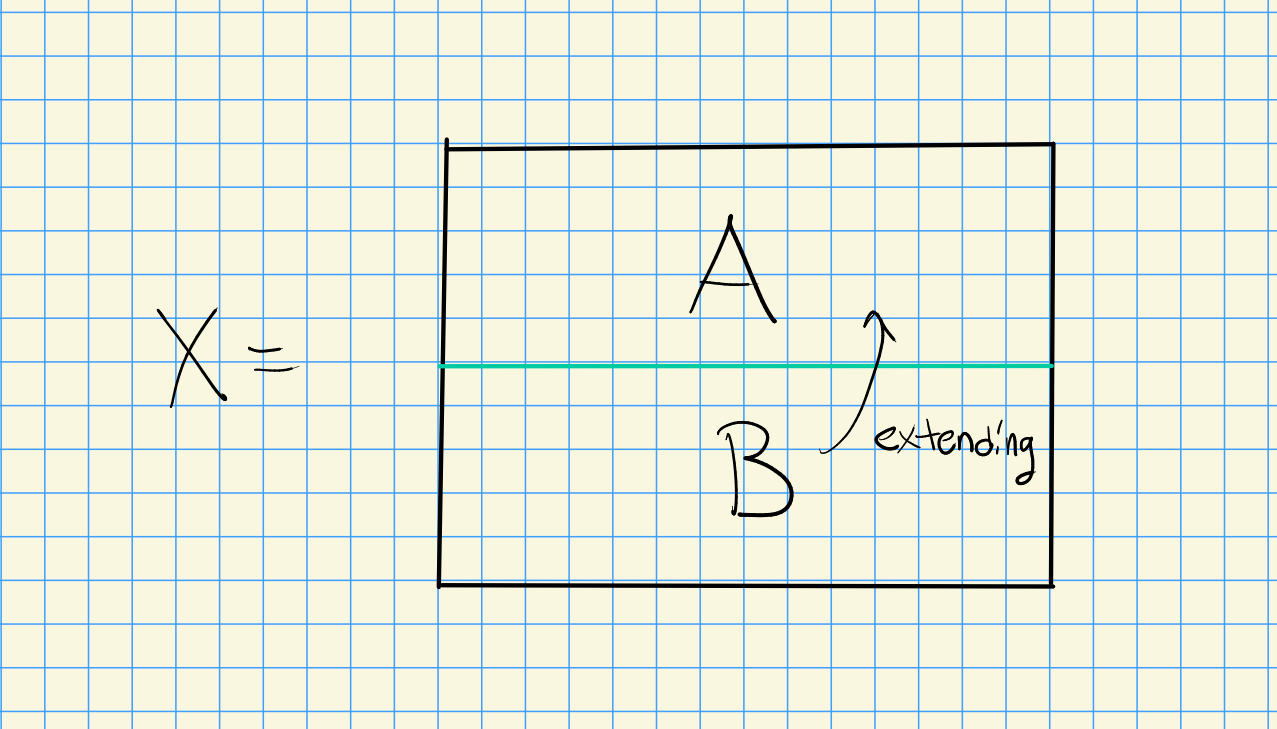
\includegraphics{figures/image_2021-02-26-09-41-27.png}
\caption{image\_2021-02-26-09-41-27}
\end{figure}

We say two extensions \(\xi, \xi'\) are equivalent and write
\(\xi \sim \xi'\) iff

\begin{center}
\begin{tikzcd}
    0 & B & X & A & 0 \\
    \\
    0 & B & {X'} & A & 0
    \arrow["\exists", dashed, from=1-3, to=3-3]
    \arrow[equals, from=1-4, to=3-4]
    \arrow[equals, from=1-2, to=3-2]
    \arrow[from=1-1, to=1-2]
    \arrow[from=1-2, to=1-3]
    \arrow[from=1-3, to=1-4]
    \arrow[from=1-4, to=1-5]
    \arrow[from=3-1, to=3-2]
    \arrow[from=3-3, to=3-4]
    \arrow[from=3-2, to=3-3]
    \arrow[from=3-4, to=3-5]
\end{tikzcd}
\end{center}

\begin{quote}
\href{https://q.uiver.app/?q=WzAsMTAsWzAsMCwiMCJdLFsxLDAsIkIiXSxbMiwwLCJYIl0sWzMsMCwiQSJdLFs0LDAsIjAiXSxbMCwyLCIwIl0sWzIsMiwiWCciXSxbMSwyLCJCIl0sWzMsMiwiQSJdLFs0LDIsIjAiXSxbMiw2LCJcXGV4aXN0cyIsMCx7InN0eWxlIjp7ImJvZHkiOnsibmFtZSI6ImRhc2hlZCJ9fX1dLFszLDgsIiIsMCx7InN0eWxlIjp7ImhlYWQiOnsibmFtZSI6Im5vbmUifX19XSxbMSw3LCIiLDAseyJzdHlsZSI6eyJoZWFkIjp7Im5hbWUiOiJub25lIn19fV0sWzAsMV0sWzEsMl0sWzIsM10sWzMsNF0sWzUsN10sWzYsOF0sWzcsNl0sWzgsOV1d}{Link
to Diagram}
\end{quote}

An extension is \textbf{split} if and only if it is equivalent to
\begin{align*}
0 \to B \overset{\iota}\hookrightarrow A \oplus B \to A 
  \xrightarrow[]{\pi} { \mathrel{\mkern-16mu}\rightarrow }\,
 A \to 0
.\end{align*}

\end{definition}

\begin{warnings}

Note that a SES as above is related to \(\operatorname{Ext}(A, B)\),
which reverses the order!

\end{warnings}

\begin{lemma}[?]

If \(\operatorname{Ext}^1(A, B) = 0\) then every extension of \(A\) by
\(B\) is split.

\end{lemma}

\begin{warnings}

There are lots of corrections needed to this proof in Weibel!

\end{warnings}

\begin{proof}[of lemma]

Given an extension \(\xi\), look at the LES associated to
\(\mathop{\mathrm{Hom}}^*({-}, B)\):

\begin{center}
\begin{tikzcd}
    && \cdots && {\operatorname{Ext}^1(A, B)} \\
    \\
    {\mathop{\mathrm{Hom}}(B, B)} && {\mathop{\mathrm{Hom}}(X, B)} && {\mathop{\mathrm{Hom}}(A, B)} \\
    \textcolor{rgb,255:red,92;green,214;blue,92}{\one_B} && \textcolor{rgb,255:red,92;green,214;blue,92}{\sigma}
    \arrow[from=3-5, to=3-3]
    \arrow[from=3-3, to=3-1]
    \arrow[from=3-1, to=1-5, out=180, in=0]
    \arrow[from=1-5, to=1-3]
    \arrow[color={rgb,255:red,92;green,214;blue,92}, maps to, from=4-3, to=4-1]
\end{tikzcd}
\end{center}

\begin{quote}
\href{https://q.uiver.app/?q=WzAsNyxbMiwwLCJcXGNkb3RzIl0sWzQsMCwiXFxFeHReMShBLCBCKSJdLFswLDIsIlxcSG9tKEIsIEIpIl0sWzIsMiwiXFxIb20oWCwgQikiXSxbNCwyLCJcXEhvbShBLCBCKSJdLFsyLDMsIlxcc2lnbWEiLFsxMjAsNjAsNjAsMV1dLFswLDMsIlxcb25lX0IiLFsxMjAsNjAsNjAsMV1dLFs0LDNdLFszLDJdLFsyLDFdLFsxLDBdLFs1LDYsIiIsMCx7ImNvbG91ciI6WzEyMCw2MCw2MF0sInN0eWxlIjp7InRhaWwiOnsibmFtZSI6Im1hcHMgdG8ifX19XV0=}{Link
to Diagram}
\end{quote}

However, this gives a splitting:

\begin{center}
\begin{tikzcd}
    & \textcolor{rgb,255:red,92;green,214;blue,92}{B} \\
    \\
    0 & B & X & A & 0 \\
    \\
    0 & B & {X'} & A & 0
    \arrow["\exists", dashed, from=3-3, to=5-3]
    \arrow[equals, from=3-4, to=5-4]
    \arrow[equals, from=3-2, to=5-2]
    \arrow[from=3-1, to=3-2]
    \arrow[from=3-2, to=3-3]
    \arrow[from=3-3, to=3-4]
    \arrow[from=3-4, to=3-5]
    \arrow[from=5-1, to=5-2]
    \arrow[from=5-3, to=5-4]
    \arrow[from=5-2, to=5-3]
    \arrow[from=5-4, to=5-5]
    \arrow["{\one_B}", color={rgb,255:red,92;green,214;blue,92}, from=3-2, to=1-2]
    \arrow["{\exists \sigma}", color={rgb,255:red,92;green,214;blue,92}, dashed, from=3-3, to=1-2]
\end{tikzcd}
\end{center}

\begin{quote}
\href{https://q.uiver.app/?q=WzAsMTEsWzAsMiwiMCJdLFsxLDIsIkIiXSxbMiwyLCJYIl0sWzMsMiwiQSJdLFs0LDIsIjAiXSxbMCw0LCIwIl0sWzIsNCwiWCciXSxbMSw0LCJCIl0sWzMsNCwiQSJdLFs0LDQsIjAiXSxbMSwwLCJCIixbMTIwLDYwLDYwLDFdXSxbMiw2LCJcXGV4aXN0cyIsMCx7InN0eWxlIjp7ImJvZHkiOnsibmFtZSI6ImRhc2hlZCJ9fX1dLFszLDgsIiIsMCx7InN0eWxlIjp7ImhlYWQiOnsibmFtZSI6Im5vbmUifX19XSxbMSw3LCIiLDAseyJzdHlsZSI6eyJoZWFkIjp7Im5hbWUiOiJub25lIn19fV0sWzAsMV0sWzEsMl0sWzIsM10sWzMsNF0sWzUsN10sWzYsOF0sWzcsNl0sWzgsOV0sWzEsMTAsIlxcb25lX0IiLDAseyJjb2xvdXIiOlsxMjAsNjAsNjBdfSxbMTIwLDYwLDYwLDFdXSxbMiwxMCwiXFxleGlzdHMgXFxzaWdtYSIsMCx7ImNvbG91ciI6WzEyMCw2MCw2MF0sInN0eWxlIjp7ImJvZHkiOnsibmFtZSI6ImRhc2hlZCJ9fX0sWzEyMCw2MCw2MCwxXV1d}{Link
to Diagram}
\end{quote}

Todo: label \((X, B) \to (B, B)\) as \(f_*\).

This is one of the many equivalent criteria for a SES of modules to be
split.

\end{proof}

\begin{remark}

More generally, given \(\xi\), let
\(\Theta(\xi) \coloneqq{{\partial}}(\one_B) \in \operatorname{Ext}^1(A, B)\).
Thus TFAE:

\begin{itemize}
\tightlist
\item
  \(\xi\) is split
\item
  \(\one-B\) lifts to some \(\sigma\in \mathop{\mathrm{Hom}}(X, B)\)
\item
  \(\one_B \in \operatorname{im}f_* = \ker {{\partial}}\)
\item
  \(\Theta(\xi) = 0\), even if \(\operatorname{Ext}^1(A, B) \neq 0\).
\end{itemize}

Then \(\Theta(\xi)\) is an \emph{obstruction} to \(\xi\) being split.

\end{remark}

\begin{remark}

If \(\xi'\sim \xi\) then
\({{\partial}}'(\one_B) = {{\partial}}(\one_B)\in \operatorname{Ext}^1(A, B)\)
by naturality of the connecting morphisms. So equivalent extensions have
the same obstruction, i.e.~\(\Theta\) only depends only on the
equivalence class \([\xi]\) of the SES.

\end{remark}

\begin{theorem}[Module extensions correspond to Ext groups]

Given \(A, B\in {\mathsf{Mod}{\hbox{-}}\mathsf{R}}\) (or an abelian
category with enough projectives and injectives), there is a
correspondence
\begin{align*}
\left\{{\substack{
  0 \to B \to X\to A \to 0
}}\right\}_{/\sim}
\mathrel{\operatorname*{\rightleftharpoons}_{\Theta}^{\Psi}}
\operatorname{Ext}^1(A, B)
\end{align*}
Note that this is a bijection of sets, but we'll upgrade it to a
bijection of abelian groups.

\end{theorem}

\hypertarget{monday-march-01}{%
\section{Monday, March 01}\label{monday-march-01}}

\begin{remark}

Last time: we looked at group extensions. Given
\(\xi: 0\to B\to X \to A\to 0\), we had a canonical element in
\(\operatorname{Ext}^1(A, B)\), namely \(\Theta(\xi) = \delta(\one_B)\).
This only depends on the equivalence class of \(\xi\).

\end{remark}

\begin{theorem}[Module extensions biject with Ext groups]

Given \(A, B\in {\mathsf{Mod}{\hbox{-}}\mathsf{R}}\), there is a
bijection
\begin{align*}
\left\{{\substack{
  \text{Extensions of $A$ by $B$}
}}\right\}
\mathrel{\operatorname*{\rightleftharpoons}_{\Theta}^{\Phi}}
\operatorname{Ext}_R^1(A, B)
\end{align*}

\end{theorem}

\begin{proof}[?]

\envlist

\begin{claim}

\(\Theta\) is surjective.

\end{claim}

Fix a SES
\begin{align*}
0 \to M \xrightarrow{j} P \xrightarrow{\pi} A \to 0 
\end{align*}
with \(P\) projective, and take the LES resulting from applying
\(\mathop{\mathrm{Hom}}({-}, B)\):

\begin{center}
\begin{tikzcd}
    0 \\
    {\mathop{\mathrm{Hom}}(A, B)} & {\mathop{\mathrm{Hom}}(P, B)} & {\mathop{\mathrm{Hom}}(M, B)} \\
    \\
    {\operatorname{Ext}^1(A, B)} & {\operatorname{Ext}^1(P, B) = 0} \\
    x
    \arrow[from=2-1, to=2-2]
    \arrow[from=2-2, to=2-3]
    \arrow["{{\partial}}", from=2-3, to=4-1, out=0, in=180]
    \arrow[from=4-1, to=4-2]
    \arrow[from=1-1, to=2-1]
\end{tikzcd}
\end{center}

\begin{quote}
\href{https://q.uiver.app/?q=WzAsNyxbMCwxLCJcXEhvbShBLCBCKSJdLFsxLDEsIlxcSG9tKFAsIEIpIl0sWzIsMSwiXFxIb20oTSwgQikiXSxbMCwzLCJcXEV4dF4xKEEsIEIpIl0sWzEsMywiXFxFeHReMShQLCBCKSA9IDAiXSxbMCw0LCJ4Il0sWzAsMCwiMCJdLFswLDFdLFsxLDJdLFsyLDMsIlxcYmQiXSxbMyw0XSxbNiwwXV0=}{Link
to Diagram}
\end{quote}

Letting \(x \in \operatorname{Ext}^1(A, B)\) and choose
\(\beta\in \mathop{\mathrm{Hom}}(M, B)\) with \({{\partial}}\beta = x\)
using that \(P\) is projective and thus \(\operatorname{Ext}^1(P, B)\)
vanishes. Now let \(X\) be the \textbf{pushout} of \(j: M\to P\) and
\(\beta: M\to B\). Note that we can apply the universal property of
cokernels to get a map of the following form:

\begin{center}
\begin{tikzcd}
    M && {P\oplus B} && {X = \operatorname{coker}g} && 0 \\
    \\
    && A
    \arrow["{g = (j, -\beta)}", from=1-1, to=1-3]
    \arrow[from=1-3, to=1-5]
    \arrow["{\pi \oplus 0}", from=1-3, to=3-3]
    \arrow[from=1-5, to=1-7]
    \arrow["{\therefore 0}"', dotted, from=1-1, to=3-3]
    \arrow["{\exists ! \mu}", dashed, from=1-5, to=3-3]
\end{tikzcd}
\end{center}

\begin{quote}
\href{https://q.uiver.app/?q=WzAsNSxbMCwwLCJNIl0sWzIsMCwiUFxcb3BsdXMgQiJdLFs0LDAsIlggPSBcXGNva2VyIGciXSxbMiwyLCJBIl0sWzYsMCwiMCJdLFswLDEsImcgPSAoaiwgLVxcYmV0YSkiXSxbMSwyXSxbMSwzLCJcXHBpIFxcb3BsdXMgMCJdLFsyLDRdLFswLDMsIlxcdGhlcmVmb3JlIDAiLDIseyJzdHlsZSI6eyJib2R5Ijp7Im5hbWUiOiJkb3R0ZWQifX19XSxbMiwzLCJcXGV4aXN0cyAhIFxcbXUiLDAseyJzdHlsZSI6eyJib2R5Ijp7Im5hbWUiOiJkYXNoZWQifX19XV0=}{Link
to Diagram}
\end{quote}

Taking the pushout yields a diagram:

\begin{center}
\begin{tikzcd}
    0 && M && P && A && 0 \\
    \\
    0 && B && X && A && 0
    \arrow[from=1-1, to=1-3]
    \arrow["j"', from=1-3, to=1-5]
    \arrow["\pi"', from=1-5, to=1-7]
    \arrow[from=3-1, to=3-3]
    \arrow["\iota"', from=3-3, to=3-5]
    \arrow["\mu"', from=3-5, to=3-7]
    \arrow[from=1-1, to=3-1]
    \arrow["\beta"', from=1-3, to=3-3]
    \arrow["\sigma"{description}, from=1-5, to=3-5]
    \arrow[equals, from=1-7, to=3-7]
    \arrow[from=1-7, to=1-9]
    \arrow[from=3-7, to=3-9]
    \arrow[from=1-9, to=3-9]
    \arrow["\lrcorner"{anchor=center, pos=0.125, rotate=180}, draw=none, from=3-5, to=1-3]
\end{tikzcd}
\end{center}

\begin{quote}
\href{https://q.uiver.app/?q=WzAsMTAsWzAsMCwiMCJdLFswLDIsIjAiXSxbMiwwLCJNIl0sWzIsMiwiQiJdLFs0LDIsIlgiXSxbNCwwLCJQIl0sWzYsMCwiQSJdLFs2LDIsIkEiXSxbOCwwLCIwIl0sWzgsMiwiMCJdLFswLDJdLFsyLDUsImoiLDJdLFs1LDYsIlxccGkiLDJdLFsxLDNdLFszLDQsIlxcaW90YSIsMl0sWzQsNywiXFxtdSIsMl0sWzAsMV0sWzIsMywiXFxiZXRhIiwyXSxbNSw0LCJcXHNpZ21hIiwxXSxbNiw3LCIiLDEseyJzdHlsZSI6eyJoZWFkIjp7Im5hbWUiOiJub25lIn19fV0sWzYsOF0sWzcsOV0sWzgsOV0sWzQsMiwiIiwyLHsic3R5bGUiOnsibmFtZSI6ImNvcm5lciJ9fV1d}{Link
to Diagram}
\end{quote}

\begin{exercise}[?]

Check that this diagram commutes and that the new row is exact.

\end{exercise}

Taking the LES for \(\mathop{\mathrm{Hom}}({-}, B)\) yields

\begin{center}
\begin{tikzcd}
    &&&& \textcolor{rgb,255:red,92;green,92;blue,214}{\beta} && \textcolor{rgb,255:red,92;green,92;blue,214}{x} \\
    \cdots && {\mathop{\mathrm{Hom}}(P, B)} && {\mathop{\mathrm{Hom}}(P, B)} && {\operatorname{Ext}^1(A, B)} \\
    \\
    \cdots && {\mathop{\mathrm{Hom}}(X, B)} && {\mathop{\mathrm{Hom}}(B, B)} && {\operatorname{Ext}^1(A, B)} \\
    &&&& \textcolor{rgb,255:red,92;green,92;blue,214}{\one_B} && \textcolor{rgb,255:red,92;green,92;blue,214}{\Theta(\xi)}
    \arrow[from=2-1, to=2-3]
    \arrow[from=2-3, to=2-5]
    \arrow[from=4-1, to=4-3]
    \arrow[from=4-3, to=4-5]
    \arrow[from=2-5, to=2-7]
    \arrow[from=4-5, to=4-7]
    \arrow[no head, from=2-7, to=4-7]
    \arrow["{\beta_*}"{description}, from=4-5, to=2-5]
    \arrow["{\sigma_*}"', from=4-3, to=2-3]
    \arrow["{{\partial}}", color={rgb,255:red,92;green,92;blue,214}, maps to, from=5-5, to=5-7]
    \arrow[color={rgb,255:red,92;green,92;blue,214}, curve={height=-30pt}, maps to, from=1-5, to=5-5]
    \arrow[color={rgb,255:red,92;green,92;blue,214}, maps to, from=1-5, to=1-7]
    \arrow[color={rgb,255:red,92;green,92;blue,214}, curve={height=-30pt}, dashed, maps to, from=1-7, to=5-7]
\end{tikzcd}
\end{center}

\begin{quote}
\((*)\)
\href{https://q.uiver.app/?q=WzAsMTIsWzIsMSwiXFxIb20oUCwgQikiXSxbNCwxLCJcXEhvbShQLCBCKSJdLFswLDEsIlxcY2RvdHMiXSxbNiwxLCJcXEV4dF4xKEEsIEIpIl0sWzIsMywiXFxIb20oWCwgQikiXSxbNCwzLCJcXEhvbShCLCBCKSJdLFs2LDMsIlxcRXh0XjEoQSwgQikiXSxbMCwzLCJcXGNkb3RzIl0sWzQsMCwiXFxiZXRhIixbMjQwLDYwLDYwLDFdXSxbNiwwLCJ4IixbMjQwLDYwLDYwLDFdXSxbNCw0LCJcXG9uZV9CIixbMjQwLDYwLDYwLDFdXSxbNiw0LCJcXFRoZXRhKFxceGkpIixbMjQwLDYwLDYwLDFdXSxbMiwwXSxbMCwxXSxbNyw0XSxbNCw1XSxbMSwzXSxbNSw2XSxbMyw2LCIiLDEseyJzdHlsZSI6eyJoZWFkIjp7Im5hbWUiOiJub25lIn19fV0sWzUsMSwiXFxiZXRhXyoiLDFdLFs0LDAsIlxcc2lnbWFfKiIsMl0sWzEwLDExLCJcXGJkIiwwLHsiY29sb3VyIjpbMjQwLDYwLDYwXSwic3R5bGUiOnsidGFpbCI6eyJuYW1lIjoibWFwcyB0byJ9fX0sWzI0MCw2MCw2MCwxXV0sWzgsMTAsIiIsMSx7ImN1cnZlIjotNSwiY29sb3VyIjpbMjQwLDYwLDYwXSwic3R5bGUiOnsidGFpbCI6eyJuYW1lIjoibWFwcyB0byJ9fX1dLFs4LDksIiIsMSx7ImNvbG91ciI6WzI0MCw2MCw2MF0sInN0eWxlIjp7InRhaWwiOnsibmFtZSI6Im1hcHMgdG8ifX19XSxbOSwxMSwiIiwxLHsiY3VydmUiOi01LCJjb2xvdXIiOlsyNDAsNjAsNjBdLCJzdHlsZSI6eyJ0YWlsIjp7Im5hbWUiOiJtYXBzIHRvIn0sImJvZHkiOnsibmFtZSI6ImRhc2hlZCJ9fX1dXQ==}{Link
to Diagram}
\end{quote}

So we

\begin{itemize}
\tightlist
\item
  Started with \(x\)
\item
  Took a reference SES
\item
  Produce the cokernel
\item
  Took a pushout and found \(\beta\).
\item
  Showed that \(\beta\mapsto x\).
\end{itemize}

\todo[inline]{Review video: 9:28 AM!}

This shows surjectivity, but depended on choice of \(\beta\).

\begin{claim}

\(\Theta\) is injective.

\end{claim}

Note that the previous construction there is a way to associate to
\(x\in \operatorname{Ext}^1(A, B)\) an extension of \(A\) by \(B\). To
see that this gives a well-defined map \(\Psi\), so
\(\Psi(x) = [ \xi ]\) as well, suppose
\(\beta'\in \mathop{\mathrm{Hom}}(M, B)\) is another lift of \(x\). Note
that although \(\operatorname{Ext}^1(P, B) =0\), the fact that
\(\ker {{\partial}}= \mathop{\mathrm{Hom}}(M, B) \neq 0\), there are
many such choices of lifts. Using exactness of diagram \((*)\), there
exists an \(f\in \mathop{\mathrm{Hom}}(P, B)\) such that
\(\beta' = \beta + fj\), recalling that \(j: M\to P\). Now taking the
pushout \(X'\) of \(j\) and \(\beta'\), the maps \(i: B\to X\) and
\(\sigma + if: P\to X\) induce an isomorphism
\(X' \xrightarrow{\sim} X\) and thus an equivalence
\(\xi \xrightarrow{\sim} \xi'\).

\begin{exercise}[?]

Check this isomorphism.

\end{exercise}

Moreover, given any extension \(\xi\), we can fit it into a diagram of
the following form:

\begin{center}
\begin{tikzcd}
    && 0 & M & P & A & 0 \\
    \\
    {\xi:} && 0 & B & X & A & 0
    \arrow[equals, from=1-6, to=3-6]
    \arrow[from=1-3, to=1-4]
    \arrow[from=1-4, to=1-5]
    \arrow[from=1-5, to=1-6]
    \arrow[from=1-6, to=1-7]
    \arrow[from=3-3, to=3-4]
    \arrow[from=3-4, to=3-5]
    \arrow[from=3-5, to=3-6]
    \arrow[from=3-6, to=3-7]
    \arrow["{\exists \beta}"{description}, dashed, from=1-4, to=3-4]
    \arrow["{\exists \sigma}"{description}, dashed, from=1-5, to=3-5]
\end{tikzcd}
\end{center}

\begin{quote}
\href{https://q.uiver.app/?q=WzAsMTEsWzIsMCwiMCJdLFszLDAsIk0iXSxbNCwwLCJQIl0sWzUsMCwiQSJdLFs2LDAsIjAiXSxbMiwyLCIwIl0sWzYsMiwiMCJdLFszLDIsIkIiXSxbNCwyLCJYIl0sWzUsMiwiQSJdLFswLDIsIlxceGk6Il0sWzMsOSwiIiwwLHsic3R5bGUiOnsiaGVhZCI6eyJuYW1lIjoibm9uZSJ9fX1dLFswLDFdLFsxLDJdLFsyLDNdLFszLDRdLFs1LDddLFs3LDhdLFs4LDldLFs5LDZdLFsxLDcsIlxcZXhpc3RzIFxcYmV0YSIsMSx7InN0eWxlIjp7ImJvZHkiOnsibmFtZSI6ImRhc2hlZCJ9fX1dLFsyLDgsIlxcZXhpc3RzIFxcc2lnbWEiLDEseyJzdHlsZSI6eyJib2R5Ijp7Im5hbWUiOiJkYXNoZWQifX19XV0=}{Link
to Diagram}
\end{quote}

First we use projectivity of \(P\) to get \(\sigma: P\to X\). Then
restricting \(\sigma\) to the kernels of \(\pi, \mu\) respectively makes
\(\beta: M\to B\), so this diagram commutes

\begin{exercise}[?]

Check that \(X\) is the pushout of \(j\) and \(\beta\).

\end{exercise}

It follows that \(\Psi (\Theta(\xi)) = \xi\) and thus \(\Theta\) is
injective, making it a bijection.

\end{proof}

\begin{remark}

Note the importance of the reversed directions after taking the Hom!

\end{remark}

\begin{remark}

How can we upgrade this to a group homomorphism? One way is to pull back
the group structure from the right-hand side to the left-hand side, but
it turns out that Baer worked out an intrinsic group structure around
1934. We can construct the ``smallest'' extension such that \(A\) is a
quotient and \(B\) is a submodule.

\end{remark}

\begin{definition}[Baer Sum (1934)]

Suppose we have two extensions of \(A\) by \(B\):
\begin{align*}
\xi: & 0\to B \xrightarrow{i} X \xrightarrow{\pi} A \to 0 \\
\xi': & 0\to B \xrightarrow{i'} X' \xrightarrow{\pi'} A \to 0 \\
.\end{align*}
Let \(X''\) be the \textbf{pullback} of \(\pi, \pi'\), defined by
\begin{align*}
X'' \coloneqq\left\{{ (x, x') \in X \times X' {~\mathrel{\Big|}~}\pi(x) = \pi'(x') \in A }\right\} 
,\end{align*}
which identifies the two copies of \(A\). This fits into a cartesian
square

\begin{center}
\begin{tikzcd}
    {X''} && {X'} \\
    \\
    X && A
    \arrow["{\pi_1}"', from=1-1, to=3-1]
    \arrow["{\pi_2}", from=1-1, to=1-3]
    \arrow["{\pi'}"', from=1-3, to=3-3]
    \arrow["\pi", from=3-1, to=3-3]
    \arrow["\lrcorner"{anchor=center, pos=0.125}, draw=none, from=1-1, to=3-3]
\end{tikzcd}
\end{center}

\begin{quote}
\href{https://q.uiver.app/?q=WzAsNCxbMCwwLCJYJyciXSxbMiwwLCJYJyJdLFsyLDIsIkEiXSxbMCwyLCJYIl0sWzAsMywiXFxwaV8xIiwyXSxbMCwxLCJcXHBpXzIiXSxbMSwyLCJcXHBpJyIsMl0sWzMsMiwiXFxwaSJdLFswLDIsIiIsMSx7InN0eWxlIjp7Im5hbWUiOiJjb3JuZXIifX1dXQ==}{Link
to Diagram}
\end{quote}

Note that \(X''\) contains 3 copies of \(B\):

\begin{itemize}
\tightlist
\item
  \(B \times 0\), or really
  \(i(B) \times\left\{{ 0 }\right\} \subset X''\) (using exactness).
\item
  \(0\times B\),
  i.e.~\(\left\{{ 0 }\right\} \times i'(B) \subseteq X''\) (using
  exactness).
\item
  \(\tilde\Delta= \left\{{ (-b, b) {~\mathrel{\Big|}~}b\in B }\right\}\),
  the \textbf{skew diagonal}. One can check that
  \(\pi i (-b) = 0 = \pi' i' (b)\).
\end{itemize}

Note that we're identifying \(B\) with \(i(B), i'(B)\). Set
\(Y \coloneqq X'' / \tilde\Delta\), then \((b, 0) + (-b, b) = (0, b)\)
where \((-b, b) \in \tilde \Delta\), so \(B \times 0\) and
\(0 \times B\) have the same image in \(Y\), since
\begin{align*}
(B \times 0) \cap\tilde\Delta= \left\{{ (0, 0) }\right\} = (0 \times B) \cap\tilde\Delta
.\end{align*}
In fact this image in \(Y\) is isomorphic to \(B\), by construction of
what we're quotienting out by. Denoting this subgroup of \(Y\) by \(B\),
we get a SES
\begin{align*}
\phi: 0\to B \to Y \to Y/B \to 0
.\end{align*}
What is \(Y/B\)? We can write this as
\begin{align*}
Y/B = { X'' / \tilde \Delta\over (0 \times B ) / \tilde\Delta}
\cong {X'' \over (0 \times B) + \tilde\Delta}
\cong {X'' / 0 \times B \over (\tilde\Delta+ (0 \times B) ) / (0 \times B)}
.\end{align*}
But the numerator is isomorphic to \(X\) by \(\pi_1\), and the
denominator is isomorphic to \(B\) by \(\pi_1\). So \(\phi\) is an
extension of \(A\) by \(B\) called the \textbf{Baer sum} of
\(\xi, \xi'\).

\end{definition}

\begin{corollary}[?]

The equivalence classes of extensions of \(A\) by \(B\) is an abelian
group under Baer sums, where zero is the class of split extensions.
Moreover, the map \(\Theta\) from the previous theorem is an isomorphism
of abelian groups.

\end{corollary}

\begin{remark}

Next time we'll check this by showing
\(\Theta(\phi) = \Theta(\xi) + \Theta(\xi')\).

\end{remark}

\hypertarget{wednesday-march-03}{%
\section{Wednesday, March 03}\label{wednesday-march-03}}

\hypertarget{baer-sum-and-higher-exts}{%
\subsection{Baer Sum and Higher Exts}\label{baer-sum-and-higher-exts}}

Last time: Baer sum.

\begin{remark}

\begin{center}
\begin{tikzcd}
    {\xi':} && 0 && B && {X'} && A && 0 \\
    \\
    {\text{Ref}:} && 0 && M && P && A && 0
    \arrow[from=1-3, to=1-5]
    \arrow["{\iota'}", from=1-5, to=1-7]
    \arrow["{\sigma'}"', from=3-7, to=1-7]
    \arrow["\pi", from=3-7, to=3-9]
    \arrow["{\pi'}", from=1-7, to=1-9]
    \arrow[from=1-9, to=1-11]
    \arrow[from=3-9, to=3-11]
    \arrow["{\beta'}", from=3-5, to=1-5]
    \arrow["j", from=3-5, to=3-7]
    \arrow[from=3-3, to=3-5]
    \arrow[equals, from=3-9, to=1-9]
\end{tikzcd}
\end{center}

\begin{quote}
\href{https://q.uiver.app/?q=WzAsMTIsWzQsMCwiQiJdLFs2LDAsIlgnIl0sWzgsMCwiQSJdLFsyLDAsIjAiXSxbNCwyLCJNIl0sWzYsMiwiUCJdLFs4LDIsIkEiXSxbMTAsMCwiMCJdLFsxMCwyLCIwIl0sWzIsMiwiMCJdLFswLDAsIlxceGknOiJdLFswLDIsIlxcdGV4dHtSZWZ9OiJdLFszLDBdLFswLDEsIlxcaW90YSciXSxbNSwxLCJcXHNpZ21hJyIsMl0sWzUsNiwiXFxwaSJdLFsxLDIsIlxccGknIl0sWzIsN10sWzYsOF0sWzQsMCwiXFxiZXRhJyJdLFs0LDUsImoiXSxbOSw0XSxbNiwyLCIiLDEseyJzdHlsZSI6eyJoZWFkIjp7Im5hbWUiOiJub25lIn19fV1d}{Link
to Diagram}
\end{quote}

\begin{center}
\begin{tikzcd}
    &&&& \textcolor{rgb,255:red,92;green,92;blue,214}{\one_B} && \textcolor{rgb,255:red,92;green,92;blue,214}{\Theta(\xi')} \\
    \cdots && {\mathop{\mathrm{Hom}}(X', B)} && {\mathop{\mathrm{Hom}}(B, B)} && {\operatorname{Ext}^1_R(A, B)} \\
    \\
    \cdots && {\mathop{\mathrm{Hom}}(P, B)} && {\mathop{\mathrm{Hom}}(M, B)} && {\operatorname{Ext}^1_R(A, B)} \\
    &&&& \textcolor{rgb,255:red,92;green,92;blue,214}{\beta'} && \textcolor{rgb,255:red,92;green,92;blue,214}{{{\partial}}(\beta') = \Theta(\xi')}
    \arrow["{\sigma'_*}", from=2-3, to=4-3]
    \arrow["{\beta'_*}", from=2-5, to=4-5]
    \arrow[from=4-1, to=4-3]
    \arrow[from=2-1, to=2-3]
    \arrow[from=2-3, to=2-5]
    \arrow[from=2-5, to=2-7]
    \arrow[from=4-3, to=4-5]
    \arrow[from=4-5, to=4-7]
    \arrow[equals, from=2-7, to=4-7]
    \arrow[color={rgb,255:red,92;green,92;blue,214}, maps to, from=5-5, to=5-7]
    \arrow[color={rgb,255:red,92;green,92;blue,214}, maps to, from=1-5, to=1-7]
    \arrow[color={rgb,255:red,92;green,92;blue,214}, curve={height=-30pt}, maps to, from=1-5, to=5-5]
    \arrow[color={rgb,255:red,92;green,92;blue,214}, curve={height=-30pt}, maps to, from=1-7, to=5-7]
\end{tikzcd}
\end{center}

\begin{quote}
\href{https://q.uiver.app/?q=WzAsMTIsWzIsMSwiXFxIb20oWCcsIEIpIl0sWzQsMSwiXFxIb20oQiwgQikiXSxbNiwxLCJcXEV4dF4xX1IoQSwgQikiXSxbNiwzLCJcXEV4dF4xX1IoQSwgQikiXSxbNCwzLCJcXEhvbShNLCBCKSJdLFsyLDMsIlxcSG9tKFAsIEIpIl0sWzAsMywiXFxjZG90cyJdLFswLDEsIlxcY2RvdHMiXSxbNCwwLCJcXG9uZV9CIixbMjQwLDYwLDYwLDFdXSxbNiwwLCJcXFRoZXRhKFxceGknKSIsWzI0MCw2MCw2MCwxXV0sWzQsNCwiXFxiZXRhJyIsWzI0MCw2MCw2MCwxXV0sWzYsNCwiXFxiZChcXGJldGEnKSA9IFxcVGhldGEoXFx4aScpIixbMjQwLDYwLDYwLDFdXSxbMCw1LCJcXHNpZ21hJ18qIl0sWzEsNCwiXFxiZXRhJ18qIl0sWzYsNV0sWzcsMF0sWzAsMV0sWzEsMl0sWzUsNF0sWzQsM10sWzIsMywiIiwxLHsic3R5bGUiOnsiaGVhZCI6eyJuYW1lIjoibm9uZSJ9fX1dLFsxMCwxMSwiIiwwLHsiY29sb3VyIjpbMjQwLDYwLDYwXSwic3R5bGUiOnsidGFpbCI6eyJuYW1lIjoibWFwcyB0byJ9fX1dLFs4LDksIiIsMCx7ImNvbG91ciI6WzI0MCw2MCw2MF0sInN0eWxlIjp7InRhaWwiOnsibmFtZSI6Im1hcHMgdG8ifX19XSxbOCwxMCwiIiwxLHsiY3VydmUiOi01LCJjb2xvdXIiOlsyNDAsNjAsNjBdLCJzdHlsZSI6eyJ0YWlsIjp7Im5hbWUiOiJtYXBzIHRvIn19fV0sWzksMTEsIiIsMSx7ImN1cnZlIjotNSwiY29sb3VyIjpbMjQwLDYwLDYwXSwic3R5bGUiOnsidGFpbCI6eyJuYW1lIjoibWFwcyB0byJ9fX1dXQ==}{Link
to Diagram}
\end{quote}

We want to define \(\xi' \oplus \xi''\), An important takeaway is that
\(\Theta\) can alternatively be defined as a map induced by the original
boundary map coming from the SES,
i.e.~\({{\partial}}(\beta') = \Theta(\xi')\). This fits into the diagram
as follows:

\begin{center}
\begin{tikzcd}
    {\xi':} && 0 && B && {X'} && A && 0 \\
    \\
    {\text{Ref}:} && 0 && M && P && A && 0 \\
    \\
    {\xi'':} && 0 && B && {X''} && A && 0
    \arrow[from=1-3, to=1-5]
    \arrow["{\iota'}", from=1-5, to=1-7]
    \arrow["{\sigma'}", from=3-7, to=1-7]
    \arrow["\pi", from=3-7, to=3-9]
    \arrow["{\pi'}", from=1-7, to=1-9]
    \arrow[from=1-9, to=1-11]
    \arrow[from=3-9, to=3-11]
    \arrow["{\beta'}", from=3-5, to=1-5]
    \arrow["j", from=3-5, to=3-7]
    \arrow[from=3-3, to=3-5]
    \arrow[equals, from=3-9, to=1-9]
    \arrow[from=5-3, to=5-5]
    \arrow["{\iota''}", from=5-5, to=5-7]
    \arrow["{\pi''}", from=5-7, to=5-9]
    \arrow[from=5-9, to=5-11]
    \arrow["{\beta''}"', from=3-5, to=5-5]
    \arrow["{\sigma''}"', from=3-7, to=5-7]
    \arrow[equals, from=3-9, to=5-9]
\end{tikzcd}
\end{center}

\begin{quote}
\href{https://q.uiver.app/?q=WzAsMTgsWzQsMCwiQiJdLFs2LDAsIlgnIl0sWzgsMCwiQSJdLFsyLDAsIjAiXSxbNCwyLCJNIl0sWzYsMiwiUCJdLFs4LDIsIkEiXSxbMTAsMCwiMCJdLFsxMCwyLCIwIl0sWzIsMiwiMCJdLFswLDAsIlxceGknOiJdLFswLDIsIlxcdGV4dHtSZWZ9OiJdLFsyLDQsIjAiXSxbNCw0LCJCIl0sWzYsNCwiWCcnIl0sWzgsNCwiQSJdLFsxMCw0LCIwIl0sWzAsNCwiXFx4aScnOiJdLFszLDBdLFswLDEsIlxcaW90YSciXSxbNSwxLCJcXHNpZ21hJyJdLFs1LDYsIlxccGkiXSxbMSwyLCJcXHBpJyJdLFsyLDddLFs2LDhdLFs0LDAsIlxcYmV0YSciXSxbNCw1LCJqIl0sWzksNF0sWzYsMiwiIiwxLHsic3R5bGUiOnsiaGVhZCI6eyJuYW1lIjoibm9uZSJ9fX1dLFsxMiwxM10sWzEzLDE0LCJcXGlvdGEnJyJdLFsxNCwxNSwiXFxwaScnIl0sWzE1LDE2XSxbNCwxMywiXFxiZXRhJyciLDJdLFs1LDE0LCJcXHNpZ21hJyciLDJdLFs2LDE1LCIiLDAseyJzdHlsZSI6eyJoZWFkIjp7Im5hbWUiOiJub25lIn19fV1d}{Link
to Diagram}
\end{quote}

We define
\begin{align*}
\tilde X \coloneqq\left\{{ (x', x'') \in X' \times X'' {~\mathrel{\Big|}~}\pi'(x') = \pi''(x'') }\right\} \twoheadrightarrow Y
,\end{align*}
and note that we had a skew diagonal \(\tilde\Delta\subseteq \tilde X\).
This yields a YES
\begin{align*}
\phi: 0 \to B \to Y \to Y/B \cong A \to 0
.\end{align*}

\end{remark}

\begin{corollary}[?]

The set of equivalence classes of extensions of \(A\) by \(B\) is an
abelian group under the Baer sum, where
\begin{align*}
[\xi] \oplus [\xi'] \coloneqq[\varphi]
,\end{align*}
where the identity element \(0\) is the class of split extensions. The
map \(\Theta\) is an isomorphism of abelian groups.

\end{corollary}

\begin{remark}

One should check that this is well-defined since we're using equivalence
classes. There is a fast way to do both at once, i.e.~showing \(\Theta\)
is well-defined and also a group morphism.

\end{remark}

\begin{proof}[?]

We'll show that
\begin{align*}
\Theta(\varphi) = \Theta(\xi) + \Theta(\xi'') \in \operatorname{Ext}^1_R(A, B)
,\end{align*}
which will make it a group isomorphism since \(\Theta\) was already a
set bijection. Considering commutativity in the 3-row diagram, we can
get a well-defined map
\begin{align*}
\sigma\coloneqq\sigma' \oplus \sigma'': P \to \tilde{X}
.\end{align*}
So let
\(\mkern 1.5mu\overline{\mkern-1.5mu \sigma\mkern-1.5mu}\mkern 1.5mu: P\to Y\)
be the induced map. The restriction of
\(\mkern 1.5mu\overline{\mkern-1.5mu \sigma\mkern-1.5mu}\mkern 1.5mu\)
to \(M\) is induced by the map
\begin{align*}
\beta' + \beta'': M\to (B \times 0) + (0 \times B) \subseteq \tilde X
.\end{align*}
These both map to \(B\) in \(Y\) under the SES
\(0\to B\to Y\to Y/B\to 0\). This gives a commutative diagram

\begin{center}
\begin{tikzcd}
    0 && M && P && A && 0 \\
    \\
    0 && B && Y && A && 0
    \arrow[equals, from=1-7, to=3-7]
    \arrow[from=1-1, to=1-3]
    \arrow[from=1-3, to=1-5]
    \arrow[from=1-5, to=1-7]
    \arrow[from=3-1, to=3-3]
    \arrow[from=3-3, to=3-5]
    \arrow[from=3-5, to=3-7]
    \arrow[from=3-7, to=3-9]
    \arrow[from=1-7, to=1-9]
    \arrow["{\beta'+\beta''}"', from=1-3, to=3-3]
    \arrow["{\mkern 1.5mu\overline{\mkern-1.5mu\sigma\mkern-1.5mu}\mkern 1.5mu}"', from=1-5, to=3-5]
\end{tikzcd}
\end{center}

\begin{quote}
\href{https://q.uiver.app/?q=WzAsMTAsWzAsMCwiMCJdLFsyLDAsIk0iXSxbNCwwLCJQIl0sWzYsMCwiQSJdLFswLDIsIjAiXSxbMiwyLCJCIl0sWzQsMiwiWSJdLFs2LDIsIkEiXSxbOCwyLCIwIl0sWzgsMCwiMCJdLFszLDcsIiIsMCx7InN0eWxlIjp7ImhlYWQiOnsibmFtZSI6Im5vbmUifX19XSxbMCwxXSxbMSwyXSxbMiwzXSxbNCw1XSxbNSw2XSxbNiw3XSxbNyw4XSxbMyw5XSxbMSw1LCJcXGJldGEnK1xcYmV0YScnIiwyXSxbMiw2LCJcXGJhcntcXHNpZ21hfSIsMl1d}{Link
to Diagram}
\end{quote}

We then have
\(\Theta(\varphi) = {{\partial}}( \beta' + \beta'') = {{\partial}}(\beta') + {{\partial}}(\beta'')\)
using that
\({{\partial}}\in \operatorname{Mor}({\mathsf{R}{\hbox{-}}\mathsf{Mod}})\).
But this is equal to \(\Theta(\xi') + \Theta(\xi'')\), which is what we
wanted to show.

\end{proof}

\begin{remark}

What about the 0 element for split SESs? Recall that additive functors
preserve split exact sequences, since these are just in terms of sums of
maps composing to the identity. Then applying the hom functor to the
original SES produces another SES, which in particular has no Ext
correction term.

\end{remark}

\begin{remark}

Similarly, \(\operatorname{Ext}^n(A, B)\) is identified with equivalence
classes of longer sequences with \(n+2\) terms, and an equivalence is a
sequence of maps that result in commuting squares:

\begin{center}
\begin{tikzcd}
    {\xi:} && 0 & B & {X_n} & \cdots & {X_1} & A & 0 \\
    \\
    {\xi':} && 0 & B & {X_n'} & \cdots & {X_1'} & A & 0
    \arrow[from=1-3, to=1-4]
    \arrow[from=1-4, to=1-5]
    \arrow[from=1-5, to=1-6]
    \arrow[from=1-6, to=1-7]
    \arrow[from=1-7, to=1-8]
    \arrow[from=1-8, to=1-9]
    \arrow[equals, from=1-4, to=3-4]
    \arrow[equals, from=1-8, to=3-8]
    \arrow[dashed, from=1-5, to=3-5]
    \arrow[dashed, from=1-7, to=3-7]
    \arrow[dashed, from=1-6, to=3-6]
    \arrow[from=3-3, to=3-4]
    \arrow[from=3-4, to=3-5]
    \arrow[from=3-5, to=3-6]
    \arrow[from=3-6, to=3-7]
    \arrow[from=3-7, to=3-8]
    \arrow[from=3-8, to=3-9]
\end{tikzcd}
\end{center}

\begin{quote}
\href{https://q.uiver.app/?q=WzAsMTYsWzIsMCwiMCJdLFszLDAsIkIiXSxbNCwwLCJYX24iXSxbNSwwLCJcXGNkb3RzIl0sWzYsMCwiWF8xIl0sWzcsMCwiQSJdLFs4LDAsIjAiXSxbMCwwLCJcXHhpOiJdLFswLDIsIlxceGknOiJdLFsyLDIsIjAiXSxbMywyLCJCIl0sWzQsMiwiWF9uJyJdLFs1LDIsIlxcY2RvdHMiXSxbNiwyLCJYXzEnIl0sWzcsMiwiQSJdLFs4LDIsIjAiXSxbMCwxXSxbMSwyXSxbMiwzXSxbMyw0XSxbNCw1XSxbNSw2XSxbMSwxMCwiIiwwLHsic3R5bGUiOnsiaGVhZCI6eyJuYW1lIjoibm9uZSJ9fX1dLFs1LDE0LCIiLDAseyJzdHlsZSI6eyJoZWFkIjp7Im5hbWUiOiJub25lIn19fV0sWzIsMTEsIiIsMCx7InN0eWxlIjp7ImJvZHkiOnsibmFtZSI6ImRhc2hlZCJ9fX1dLFs0LDEzLCIiLDAseyJzdHlsZSI6eyJib2R5Ijp7Im5hbWUiOiJkYXNoZWQifX19XSxbMywxMiwiIiwwLHsic3R5bGUiOnsiYm9keSI6eyJuYW1lIjoiZGFzaGVkIn19fV0sWzksMTBdLFsxMCwxMV0sWzExLDEyXSxbMTIsMTNdLFsxMywxNF0sWzE0LDE1XV0=}{Link
to Diagram}
\end{quote}

Note that if \({P}_{*} \to A\to 0\) is a projective resolution, then the
comparison theorem yields maps and a commutative diagram

\begin{center}
\begin{tikzcd}
    {\phi:} && 0 & M & {P_{n-1}} & \cdots & {P_0} & A & 0 \\
    \\
    {\xi':} && 0 & B & {X_n'} & \cdots & {X_1'} & A & 0
    \arrow[from=1-3, to=1-4]
    \arrow[from=1-4, to=1-5]
    \arrow[from=1-5, to=1-6]
    \arrow[from=1-6, to=1-7]
    \arrow[from=1-7, to=1-8]
    \arrow[from=1-8, to=1-9]
    \arrow["{\exists \beta}", dashed, from=1-4, to=3-4]
    \arrow["{\one_A}", equals, from=1-8, to=3-8]
    \arrow["\exists", dashed, from=1-5, to=3-5]
    \arrow["\exists", dashed, from=1-7, to=3-7]
    \arrow[dashed, from=1-6, to=3-6]
    \arrow[from=3-3, to=3-4]
    \arrow[from=3-4, to=3-5]
    \arrow[from=3-5, to=3-6]
    \arrow[from=3-6, to=3-7]
    \arrow[from=3-7, to=3-8]
    \arrow[from=3-8, to=3-9]
\end{tikzcd}
\end{center}

\begin{quote}
\href{https://q.uiver.app/?q=WzAsMTYsWzIsMCwiMCJdLFszLDAsIk0iXSxbNCwwLCJQX3tuLTF9Il0sWzUsMCwiXFxjZG90cyJdLFs2LDAsIlBfMCJdLFs3LDAsIkEiXSxbOCwwLCIwIl0sWzAsMCwiXFxwaGk6Il0sWzAsMiwiXFx4aSc6Il0sWzIsMiwiMCJdLFszLDIsIkIiXSxbNCwyLCJYX24nIl0sWzUsMiwiXFxjZG90cyJdLFs2LDIsIlhfMSciXSxbNywyLCJBIl0sWzgsMiwiMCJdLFswLDFdLFsxLDJdLFsyLDNdLFszLDRdLFs0LDVdLFs1LDZdLFsxLDEwLCJcXGV4aXN0cyBcXGJldGEiLDAseyJzdHlsZSI6eyJib2R5Ijp7Im5hbWUiOiJkYXNoZWQifX19XSxbNSwxNCwiXFxvbmVfQSIsMCx7InN0eWxlIjp7ImhlYWQiOnsibmFtZSI6Im5vbmUifX19XSxbMiwxMSwiXFxleGlzdHMiLDAseyJzdHlsZSI6eyJib2R5Ijp7Im5hbWUiOiJkYXNoZWQifX19XSxbNCwxMywiXFxleGlzdHMiLDAseyJzdHlsZSI6eyJib2R5Ijp7Im5hbWUiOiJkYXNoZWQifX19XSxbMywxMiwiIiwwLHsic3R5bGUiOnsiYm9keSI6eyJuYW1lIjoiZGFzaGVkIn19fV0sWzksMTBdLFsxMCwxMV0sWzExLDEyXSxbMTIsMTNdLFsxMywxNF0sWzE0LDE1XV0=}{Link
to Diagram}
\end{quote}

Then the dimension shifting theorem (Exc. 2.4.3) and its proof yields an
exact sequence
\begin{align*}
\mathop{\mathrm{Hom}}(P_{n-1}, B) \to \mathop{\mathrm{Hom}}(M, B) \xrightarrow{{{\partial}}} \operatorname{Ext}^n(A, B) \to 0
,\end{align*}
and the asserted bijection is then given by
\(\Theta(\xi) \coloneqq{{\partial}}(\beta)\).

\end{remark}

\hypertarget{kunneth-and-universal-coefficient-theorems}{%
\subsection{3.6: Kunneth and Universal Coefficient
Theorems}\label{kunneth-and-universal-coefficient-theorems}}

\begin{observation}

If \(R\) is a field \(F\) then \(\operatorname{Tor}_n^F(A, B) = 0\) for
all \(n>0\), i.e.~every module over a field is a complex space, hence
free, hence projective, hence flat, and so \(A\otimes_F {-}\) is exact.

\end{observation}

\begin{question}

If \({P}_{*} \in \mathsf{Ch}({\mathsf{Mod}{\hbox{-}}\mathsf{R}})\) is a
complex of of right \(R{\hbox{-}}\)modules and
\(M \in {\mathsf{R}{\hbox{-}}\mathsf{Mod}}\) is a left
\(R{\hbox{-}}\)module, how is the homology of \({P}_{*}\) and that of
\({P}_{*} \otimes_R M\) related?

\end{question}

\begin{lemma}[?]

Given a 5-term exact sequence
\begin{align*}
A_1 \xrightarrow{\alpha} A_2 \xrightarrow{f} B \xrightarrow{g} C_1 \xrightarrow{\gamma} C_2
,\end{align*}
there is a corresponding SES

\begin{center}
\begin{tikzcd}
    0 & A & B & C & 0 \\
    & {\substack{ A_2/\ker f = A_2/\operatorname{im}\alpha \\ = \operatorname{coker}\alpha} } && {\operatorname{im}g = \ker f}
    \arrow[from=1-1, to=1-2]
    \arrow["{\mkern 1.5mu\overline{\mkern-1.5muf\mkern-1.5mu}\mkern 1.5mu}", from=1-2, to=1-3]
    \arrow["g", from=1-3, to=1-4]
    \arrow[from=1-4, to=1-5]
\end{tikzcd}
\end{center}

\begin{quote}
\href{https://q.uiver.app/?q=WzAsNyxbMCwwLCIwIl0sWzEsMCwiQSJdLFsyLDAsIkIiXSxbMywwLCJDIl0sWzQsMCwiMCJdLFszLDEsIlxcaW0gZyA9IFxca2VyIGYiXSxbMSwxLCJBXzIvXFxrZXIgZiA9IEFfMi9cXGltXFxhbHBoYSA9IFxcY29rZXIgXFxhbHBoYSJdLFswLDFdLFsxLDIsIlxcYmFyIGYiXSxbMiwzLCJnIl0sWzMsNF1d}{Link
to Diagram}
\end{quote}

In particular, we can always take \(A = \operatorname{coker}\alpha\) and
\(C = \ker \gamma\) in any abelian category.

\end{lemma}

\begin{theorem}[The Kunneth Formula]

Let \({P}_{*}\in \mathsf{Ch}({\mathsf{Mod}{\hbox{-}}\mathsf{R}})\) be a
chain complex of flat right \(R{\hbox{-}}\)modules such that each
boundary module \(dP_n\) is again flat. Then for every
\(M\in {\mathsf{R}{\hbox{-}}\mathsf{Mod}}\) and all \(N\), there is an
exact sequence

\begin{center}
\begin{tikzcd}
    0 && {H_n({P}_{*})\otimes_R M} && {H_n({P}_{*} \otimes_R M)} && {\operatorname{Tor}^1_R(H_{n-1}({P}_{*}), M)} && 0
    \arrow[from=1-7, to=1-9]
    \arrow[from=1-5, to=1-7]
    \arrow[from=1-3, to=1-5]
    \arrow[from=1-1, to=1-3]
\end{tikzcd}
\end{center}

\begin{quote}
\href{https://q.uiver.app/?q=WzAsNSxbMCwwLCIwIl0sWzIsMCwiSF9uKFxcdmVjdG9yIFApXFx0ZW5zb3JfUiBNIl0sWzQsMCwiSF9uKFxcdmVjdG9yIFAgXFx0ZW5zb3JfUiBNKSJdLFs2LDAsIlxcVG9yXjFfUihIX3tuLTF9KFxcdmVjdG9yIFApLCBNKSJdLFs4LDAsIjAiXSxbMyw0XSxbMiwzXSxbMSwyXSxbMCwxXV0=}{Link
to Diagram}
\end{quote}

\end{theorem}

\begin{remark}

Note that the correction term vanishes if \(R\) is a field.

\end{remark}

\begin{proof}[?]

Let \(Z_n \coloneqq Z_n({P}_{*})\), there there is a SES
\begin{align*}
0 \to Z_n \to P_n \xrightarrow{d} dP_n \to 0
.\end{align*}
Since \(P_n, dP_n\) are flat by assumption, by Exc. 3.2.2, \(Z_n\) is
also flat. Taking the LES from applying \({-}\otimes_R M\), noting that
\(M\) is arbitrary yields

\begin{center}
\begin{tikzcd}
    &&&& 0 \\
    {Z_n\otimes_R M} && {P_n\otimes_R M} && {dP_n\otimes_R M} \\
    \\
    && \cdots && {\operatorname{Tor}_1(dP_n, M)}
    \arrow[from=4-5, to=2-1, out=0, in=180]
    \arrow[from=2-1, to=2-3]
    \arrow[from=2-3, to=2-5]
    \arrow[from=4-3, to=4-5]
    \arrow[from=2-5, to=1-5]
\end{tikzcd}
\end{center}

\begin{quote}
\href{https://q.uiver.app/?q=WzAsNixbNCwxLCJkUF9uXFx0ZW5zb3JfUiBNIl0sWzIsMSwiUF9uXFx0ZW5zb3JfUiBNIl0sWzAsMSwiWl9uXFx0ZW5zb3JfUiBNIl0sWzQsMywiXFxUb3JfMShkUF9uLCBNKSJdLFsyLDMsIlxcY2RvdHMiXSxbNCwwLCIwIl0sWzMsMl0sWzIsMV0sWzEsMF0sWzQsM10sWzAsNV1d}{Link
to Diagram}
\end{quote}

Here \(\operatorname{Tor}_1(dP_n, M)=0\) since \(dP_n\) is flat, noting
that one could also apply \(\operatorname{Tor}(dP_n, {-})\) to get a
similar LES. So this lifts to a SES of complexes
\begin{align*}
0 \to {Z}_{*}\otimes M \to {P}_{*}\otimes M \to {dP}_{*}\otimes M \to 0
,\end{align*}
where we can consider \(d\otimes\one\) in the middle. We'll pick this up
next time!

\end{proof}

\hypertarget{friday-march-05}{%
\section{Friday, March 05}\label{friday-march-05}}

\begin{quote}
See first 10m
\end{quote}

\begin{observation}

For a SES
\begin{align*}
A_1 \xrightarrow{\alpha} A_2 \xrightarrow{f} B \xrightarrow{g} C_1 \xrightarrow{\gamma} C_2
,\end{align*}
one can obtain an exact sequence
\begin{align*}
0\to \operatorname{coker}\alpha \xrightarrow{\mkern 1.5mu\overline{\mkern-1.5muf\mkern-1.5mu}\mkern 1.5mu} B \xrightarrow{g} \ker \gamma \to 0
.\end{align*}

\end{observation}

\begin{observation}

For a SES
\begin{align*}
0 \to Y \xrightarrow{i} Z \xrightarrow{\pi} {Z\over Y} \to 0
\end{align*}
there is an induced exact sequence

\end{observation}

Some missed stuff here.

\begin{proof}[of Kunneth Formula (continued)]

Note that
\begin{align*}
0\to {Z}_{*} \otimes M \to {P}_{*}\otimes M \to d{P}_{*}\otimes M\to 0
,\end{align*}
where the differentials for the end terms are zero, and the homology
will recover the original complex.

\begin{center}
\begin{tikzcd}
    &&&& {} && {H_{n+1}(dP \otimes M)= dP \otimes M} \\
    \\
    {} && {H_{n}(Z \otimes M) = Z\otimes M} && {H_{n}(P \otimes M)} && {H_{n}(dP \otimes M) = dP \otimes M} \\
    \\
    && {H_{n-1}(Z \otimes M) = Z_{n-1}\otimes M}
    \arrow[from=1-7, to=3-3, in=180, out=0]
    \arrow[from=3-3, to=3-5]
    \arrow[from=3-5, to=3-7]
    \arrow[from=3-7, to=5-3, in=180, out=0]
\end{tikzcd}
\end{center}

\begin{quote}
\href{https://q.uiver.app/?q=WzAsNyxbMCwyXSxbMiwyLCJIX3tufShaIFxcdGVuc29yIE0pID0gWlxcdGVuc29yIE0iXSxbNCwyLCJIX3tufShQIFxcdGVuc29yIE0pIl0sWzQsMF0sWzYsMCwiSF97bisxfShkUCBcXHRlbnNvciBNKT0gZFAgXFx0ZW5zb3IgTSJdLFs2LDIsIkhfe259KGRQIFxcdGVuc29yIE0pID0gZFAgXFx0ZW5zb3IgTSJdLFsyLDQsIkhfe24tMX0oWiBcXHRlbnNvciBNKSA9IFpfe24tMX1cXHRlbnNvciBNIl0sWzQsMV0sWzEsMl0sWzIsNV0sWzUsNl1d}{Link
to Diagram}
\end{quote}

By using the explicit formula for \({{\partial}}\), it turns out that
\({{\partial}}= (dP_{i+1} \overset{i}\hookrightarrow Z) \otimes\one M\).
By observation one, we get a SES
\begin{align*}
0 \to {Z_n\otimes M \over dP_{n+1} \otimes M } \to H_n(P\otimes M) \to \ker i( \otimes\one_M) \to 0
.\end{align*}

By observation 1, the first term equals \(H_n({P}_{*})\otimes M\). From
this, we get a flat resolution of \(H_{n-1}(P)\):

\begin{center}
\begin{tikzcd}
    \textcolor{rgb,255:red,214;green,92;blue,92}{\deg:} & \textcolor{rgb,255:red,214;green,92;blue,92}{2} & \textcolor{rgb,255:red,214;green,92;blue,92}{1} & \textcolor{rgb,255:red,214;green,92;blue,92}{0} \\
    0 & 0 & {dP_n} & {Z_{n-1}} & {H_{n-1}(P)} & 0
    \arrow[from=2-2, to=2-3]
    \arrow[from=2-3, to=2-4]
    \arrow[from=2-4, to=2-5]
    \arrow[from=2-5, to=2-6]
    \arrow[from=2-1, to=2-2]
\end{tikzcd}
\end{center}

\begin{quote}
\href{https://q.uiver.app/?q=WzAsMTAsWzAsMSwiMCJdLFsxLDEsIjAiXSxbMSwwLCIyIixbMCw2MCw2MCwxXV0sWzIsMCwiMSIsWzAsNjAsNjAsMV1dLFszLDAsIjAiLFswLDYwLDYwLDFdXSxbMiwxLCJkUF9uIl0sWzMsMSwiWl97bi0xfSJdLFs0LDEsIkhfe24tMX0oUCkiXSxbNSwxLCIwIl0sWzAsMCwiXFxkZWc6IixbMCw2MCw2MCwxXV0sWzEsNV0sWzUsNl0sWzYsN10sWzcsOF0sWzAsMV1d}{Link
to Diagram}
\end{quote}

So we can use this to compute \(\operatorname{Tor}(H_{n-1}(P), M)\) by
taking homology:

\begin{center}
\begin{tikzcd}
    \textcolor{rgb,255:red,214;green,92;blue,92}{\deg} & \textcolor{rgb,255:red,214;green,92;blue,92}{2} & \textcolor{rgb,255:red,214;green,92;blue,92}{1} & \textcolor{rgb,255:red,214;green,92;blue,92}{0} \\
    0 & 0 & {dP_n \otimes M} & {Z_{n-1}\otimes M} & 0
    \arrow[from=2-1, to=2-2]
    \arrow[from=2-2, to=2-3]
    \arrow["{i\otimes\one}", from=2-3, to=2-4]
    \arrow[from=2-4, to=2-5]
\end{tikzcd}
\end{center}

\begin{quote}
\href{https://q.uiver.app/?q=WzAsOSxbMCwxLCIwIl0sWzEsMSwiMCJdLFsyLDEsImRQX24gXFx0ZW5zb3IgTSJdLFszLDEsIlpfe24tMX1cXHRlbnNvciBNIl0sWzQsMSwiMCJdLFszLDAsIjAiLFswLDYwLDYwLDFdXSxbMiwwLCIxIixbMCw2MCw2MCwxXV0sWzEsMCwiMiIsWzAsNjAsNjAsMV1dLFswLDAsIlxcZGVnIixbMCw2MCw2MCwxXV0sWzAsMV0sWzEsMl0sWzIsMywiaVxcdGVuc29yIFxcMSJdLFszLDRdXQ==}{Link
to Diagram}
\end{quote}

Thus
\begin{align*}
\ker(i\otimes\one_M) = \operatorname{Tor}_1( H_{n-1}(P), M) \cong \ker (dP_m \xrightarrow{{{\partial}}} Z_{n-1} \otimes M)
.\end{align*}

\end{proof}

\begin{theorem}[Universal Coefficient Theorem]

Let \({P}_{*}\) be a chain complex of free abelian groups. For every
abelian groups \(M\) and every \(n\), the Kunneth sequence splits
non-canonically as
\begin{align*}
H_n({P}_{*} \otimes M) \cong \qty{ H_n( {P}_{*} )\otimes M } \oplus \operatorname{Tor}_1^{{\mathbb{Z}}}(H_{n-1}(P), M)
.\end{align*}

\end{theorem}

\begin{remark}

In optimal situations the tor term vanishes, e.g.~if either term is
torsionfree (so no elements of finite order).

\end{remark}

\begin{fact}

Every subgroup of a free abelian group is free (hence projective, hence
flat).

\end{fact}

\begin{proof}[?]

Since \(dP_n \leq dP_{n-1}\), we can conclude \(dP_n\) is free. Thus the
following SES splits:
\begin{align*}
0\to Z_n \to P_n \xrightarrow{d} dP_n \to 0
.\end{align*}
So any lift of the identity map on \(dP_n\) gives an isomorphic copy of
the last term in the middle term, yielding
\(P_n \cong Z_n \oplus dP_n\). Now tensoring with \(M\) and using that
it distributes over direct sums yields
\begin{align*}
P_n \otimes M \cong (Z_n \otimes M) \oplus (dP_n \otimes M)
.\end{align*}
The left-hand side contains a copy of
\(\ker(d_n \otimes\one: P_n \otimes M \to P_{n-1} \otimes M)\), which
itself contains a copy of \(Z_n\otimes M\). So by a linear algebra
exercise, we have
\(\ker(d_n \otimes\one) \cong (Z_n \otimes M) \oplus A\) for some
unknown \(A\), and since
\(dP_{n+1} \otimes M = \operatorname{im}(d_{n+1}\otimes\one)\) is
contained in the first term, we can use the partial exactness of
tensoring to preserve quotients and obtain
\begin{align*}
H_n(P\otimes M) = \qty{ H_n(P) \otimes M}  \oplus C'
\end{align*}
for some \(C'\). Now applying the Kunneth formula we find that
\(C' = \operatorname{Tor}^{\mathbb{Z}}_1( H_{n-1}(P), M)\), yielding the
claimed direct sum.

\end{proof}

\begin{remark}

The following is a generalization for both.

\end{remark}

\begin{theorem}[Kunneth formula for complexes]

Let \(P, Q \in \mathsf{Ch}({\mathsf{R}{\hbox{-}}\mathsf{Mod}})\) be
complexes, then
\begin{align*}
P\otimes Q \coloneqq\operatorname{Tot}^{\oplus}(P\otimes Q)_n \coloneqq\bigoplus_{p+q = n} P_p \otimes Q_q
\end{align*}
with differential\footnote{Recall that the squares would commute if we
  took the usual differentials, so we use a sign trick to get \(d^2=0\).}
\begin{align*}
d(a\otimes b) = (da)\otimes b + (-1)^pa \otimes(db)
.\end{align*}
If \(P_n, dP_n\) are flat for all \(n\), then there exists a SES
\begin{align*}
0 
\to \bigoplus_{p+q=n} H_p(P)\otimes H_q(Q) 
\to H_n(P\otimes Q) 
\to \bigoplus_{p+q=n-1} \operatorname{Tor}^R_1(H_p(P), H_q(Q) ) 
\to 0
.\end{align*}

\end{theorem}

\begin{proof}[?]

Omitted here, but uses same ideas as the previous proofs. Hint: take
\(Q\) to have \(M\) in degree 0.

\end{proof}

\hypertarget{applications-to-topology}{%
\subsection{Applications to Topology}\label{applications-to-topology}}

\begin{definition}[Simplicial Homology]

See some applications in section 1 of Weibel, e.g.~simplicial and
singular homology. The setup:
\(X\in {\mathsf{Top}}, R\in \mathsf{Ring}\) unital, and for \(k\geq 0\)
let \(S_k = S_k(X)\) be the free \(R{\hbox{-}}\)module on
\(\mathop{\mathrm{Hom}}_{\mathsf{Top}}( \Delta_k, X)\) where
\(\Delta_k\) is the standard simplex By ordering the vertices, this
induces an ordering on the faces by taking lexicographic ordering. Then
the restriction of a map \(\Delta_k \to X\) to the \(i\)th face of
\(\Delta_k\) gives a map \(\Delta_{k-1} \to X\), which induces an
\(R{\hbox{-}}\)module morphism \({{\partial}}_i: S_k \to S_{k-1}\) By
summing these we can define
\(d \coloneqq\sum_{i=0}^k (-1)^i {{\partial}}_i: S_k\to S_{k-1}\) and it
turns out that \(d^2 = 0\). So we can define a complex
\begin{align*}
\cdots \to S_2 \xrightarrow{d} \to S_1\to S_0 \to 0 \in \mathsf{Ch}({\mathsf{R}{\hbox{-}}\mathsf{Mod}})
.\end{align*}
Taking it homology yields the \textbf{simplicial homology} of the
complex \(H_n(X; R) \coloneqq H_n({S}_{*}(X) )\).

\end{definition}

\begin{remark}

Taking \(R={\mathbb{Z}}\) makes \(S_k(X)\) a free abelian group. If
\(M\) is any abelian group, we can define
\(H_n(X; M) \coloneqq H_n( {S}_{*}(X) \otimes_{\mathbb{Z}}M)\), the
homology with \textbf{coefficients} in \(M\). If no coefficients are
specified, we write \(H_n(X) \coloneqq H_n(X; {\mathbb{Z}})\). There is
then a universal coefficient theorem in topology:
\begin{align*}
H_n(X; M) 
\cong 
\qty{ H_n(X) \otimes_{\mathbb{Z}}M} \oplus \operatorname{Tor}_1^{\mathbb{Z}}( H_{n-1}(X), M)
.\end{align*}

\end{remark}

\begin{remark}

Next week: group cohomology, spectral sequences next week. This will
give us some objects to apply spectral sequences.

\end{remark}

\hypertarget{monday-march-08}{%
\section{Monday, March 08}\label{monday-march-08}}

\hypertarget{universal-coefficients-theorem}{%
\subsection{3.6: Universal Coefficients
Theorem}\label{universal-coefficients-theorem}}

\begin{remark}

Let \(X \in {\mathsf{Top}}\) and \(S_k(X)\) be the free
\({\mathbb{Z}}{\hbox{-}}\)module on
\(\mathop{\mathrm{Hom}}_{\mathsf{Top}}( \Delta_k, X)\), which assemble
into a chain complex \(S(X)\). For \(M\in {\mathsf{Ab}}\), we defined
\(H^n(X; M) \coloneqq H^n( \mathop{\mathrm{Hom}}(S(X), M))\) and write
\(H^n(X) \coloneqq H^n(X; {\mathbb{Z}})\). The universal coefficient
theorem states
\begin{align*}
H^n(X; M) \cong \mathop{\mathrm{Hom}}_{\mathbb{Z}}(H_n(X), M) \oplus \operatorname{Ext}^1_{\mathbb{Z}}( H_{n-1}(X), M)
.\end{align*}

\end{remark}

\begin{warnings}

Note that this is homology on the RHS, not cohomology!

\end{warnings}

\begin{theorem}[Universal Coefficients Theorem for Cohomology]

Let \({P}_{*}\) be a chain complex of projective \(R{\hbox{-}}\)modules.
Assume \(dP_n\) is also projective for all \(n\). For
\(M\in {\mathsf{R}{\hbox{-}}\mathsf{Mod}}\), there is a split SES
\begin{align*}
0 \to \operatorname{Ext}_R^1(H_{n-1}(P), M) \to H^n( \mathop{\mathrm{Hom}}_R( {P}_{*}, M)) \to \mathop{\mathrm{Hom}}_R (H_n(P), M) \to 0
.\end{align*}

\end{theorem}

\todo[inline]{Ask about naturality!}

\begin{proof}[Sketch]

As in the last lecture with free abelian groups, since the \(dP_n\) are
projective we can split \(P_n \cong Z_n \oplus dP_n\) since
\(Z_n = \ker d\). Applying homs, since it's an additive functor this
yields a new split exact sequence
\begin{align*}
0 \to \mathop{\mathrm{Hom}}(dP_n, M) \to \mathop{\mathrm{Hom}}(P_n, M) \to \mathop{\mathrm{Hom}}(Z_n, M) \to 0
.\end{align*}
Now running the proof for the original Kunneth formula and replacing
tensor products to homs, these assemble into a split exact sequence of
complexes and this yields the desired SES. Using the strategy of the
proof of the UCF for free abelian groups to see that the sequence splits
(although non-canonically).

\end{proof}

\begin{remark}

Note that flat is weaker than projective for tensor products, but in an
asymmetric situation, there's nothing weaker than projective for the hom
functors to be exact (since this is an iff).

\end{remark}

\hypertarget{ch.-6-group-homology-and-cohomology}{%
\subsection{Ch. 6: Group Homology and
Cohomology}\label{ch.-6-group-homology-and-cohomology}}

\hypertarget{definitions-and-properties}{%
\subsubsection{Definitions and
Properties}\label{definitions-and-properties}}

\begin{definition}[Modules of Groups]

Let \(G\in {\mathsf{Grp}}\) be any group, finite or infinite, and let
\(A\in \mathsf{G}{\hbox{-}}\mathsf{Mod}\) be a left
\(G{\hbox{-}}\)module, i.e.~an abelian group on which \(G\) acts by
additive maps on the left, written \(g.a\) or \(ga\) for
\(g\in G, a\in A\). Here \emph{additive} means that
\(g.(a_1 + a_2) = g.a_1 + g.a_2\). Note that this implies
\(g.0 = 0, -g.a = -(g.a), g_1 (g_2 . a) = (g_1 g_2).a, 1_G.a = a\).
Writing
\(\mathop{\mathrm{End}}_R(A) \coloneqq\mathop{\mathrm{Hom}}_R(A, A)\),
we have a group morphism
\begin{align*}
G &\to \mathop{\mathrm{End}}_{\mathbb{Z}}(A) \\
g &\mapsto g.({-})
.\end{align*}

\end{definition}

\begin{definition}[Equivariant Maps]

If \(B \in \mathsf{G}{\hbox{-}}\mathsf{Mod}\) is another left
\(G{\hbox{-}}\)module, then
\begin{align*}
\mathop{\mathrm{Hom}}_G(A, B) = \left\{{ f\in \mathop{\mathrm{Hom}}_{\mathbb{Z}}(A, B) {~\mathrel{\Big|}~}f(g.a) = g(f(a)) \quad \forall a\in A, \forall g\in G }\right\} 
,\end{align*}
which are \textbf{\(G{\hbox{-}}\)equivariant maps}.

\end{definition}

\begin{definition}[Integral Group Ring]

We define
\begin{align*}
{\mathbb{Z}}G\coloneqq\left\{{ \sum_{i=1}^N m_i g_i {~\mathrel{\Big|}~}m_i\in {\mathbb{Z}}, g_i\in G, n\in {\mathbb{N}}}\right\} 
.\end{align*}
We can equip this with a ring structure using \((mg)(m' g') = mm' gg'\)
and extending \({\mathbb{Z}}{\hbox{-}}\)linearly.

\end{definition}

\begin{remark}

There is an equality of categories
\({\mathsf{G}{\hbox{-}}\mathsf{Mod}} = \mathsf{{\mathbb{Z}}G}{\hbox{-}}\mathsf{Mod}\).
This is also the same as the functor category
\({\mathsf{Ab}}^\mathcal{G}\) (a category of the form
\(\mathcal{A}^{\mathcal{I}}\)) where \(\mathcal{G}\) is the category
with one object whose morphisms are the elements of \(G\). In other
words,
\({\operatorname{Ob}}(\mathcal{G}) \coloneqq\left\{{ 1 }\right\}\) and
\(\mathop{\mathrm{Hom}}_{\mathcal{G}}(1, 1) = G\). Note that every
morphism is invertible since \(G\) is a group.

\begin{figure}
\centering
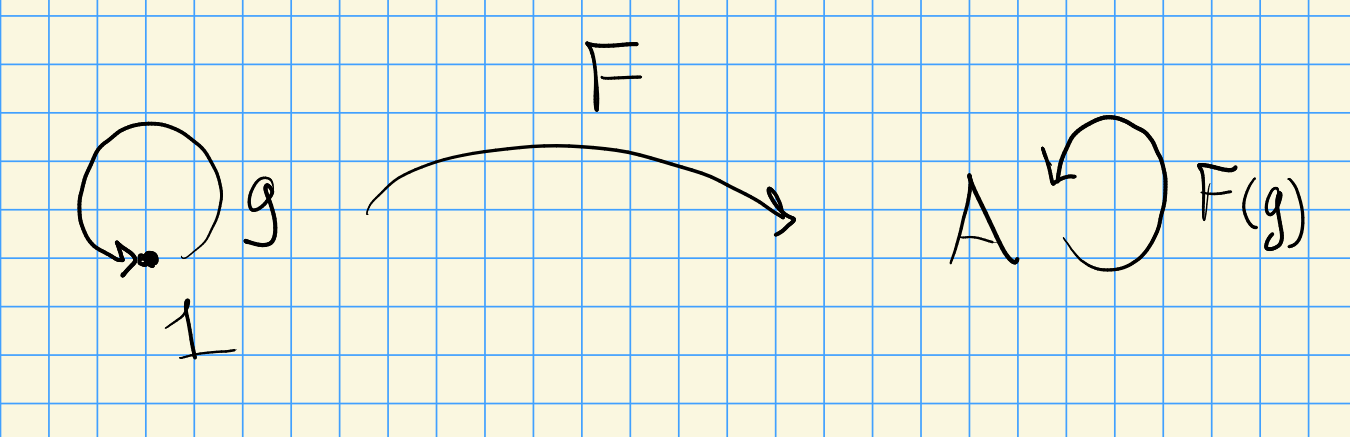
\includegraphics{figures/image_2021-03-08-09-36-58.png}
\caption{image\_2021-03-08-09-36-58}
\end{figure}

The right-hand side yields a \(G{\hbox{-}}\)module since
\(F(g)(a) = g.a\).

\end{remark}

\begin{definition}[Trivial modules]

An object \(A\in \mathsf{G}{\hbox{-}}\mathsf{Mod}\) is a
\textbf{trivial} module if and only if \(g.a = a\) for all \(g\in G\).

\end{definition}

\begin{remark}

Any \(G\in {\mathsf{Ab}}\) can be viewed as a trivial
\(G{\hbox{-}}\)module in this way. This yields a functor
\(\operatorname{Triv}:{\mathsf{Ab}}\to \mathsf{G}{\hbox{-}}\mathsf{Mod}\).
There is a distinguished trivial \(G{\hbox{-}}\)module, namely
\(A \coloneqq{\mathbb{Z}}\) with the trivial \(G{\hbox{-}}\)action.
There are two natural functors
\(\mathsf{G}{\hbox{-}}\mathsf{Mod}\to {\mathsf{Ab}}\):

\begin{itemize}
\tightlist
\item
  \(A^G \coloneqq\left\{{ a\in A {~\mathrel{\Big|}~}g.a = a \forall g\in G }\right\}\),
  the \textbf{invariant subgroup} of \(A\).
\item
  \(A_G \coloneqq A / \left\langle{ ga-a {~\mathrel{\Big|}~}g\in G, a\in A }\right\rangle\),
  where we take the \(G{\hbox{-}}\)module generated by the relation in
  the denominator, which are the \textbf{coinvariants} of \(A\).
\end{itemize}

\end{remark}

\begin{exercise}[6.1.1]

\envlist

\begin{enumerate}
\def\labelenumi{\arabic{enumi}.}
\item
  \(A^G\) is the maximal trivial submodule of \(A\), so the functor
  \(({-})^G\) is right-adjoint to \(\operatorname{Triv}\). These should
  both be easy checks! So this is left-exact and has right-derived
  functors (similar to ext).
\item
  \(A_G\) is the largest \(G{\hbox{-}}\)trivial quotient of \(A\), and
  \(({-})_G\) is left-adjoint to \(\operatorname{Triv}\). Thus it is
  right-exact and has left-derived functors (similar to tor).
\end{enumerate}

\end{exercise}

\begin{lemma}[?]

Let \(A\in \mathsf{G}{\hbox{-}}\mathsf{Mod}\) and \({\mathbb{Z}}\) be
the trivial \(G{\hbox{-}}\)module. Then

\begin{enumerate}
\def\labelenumi{\arabic{enumi}.}
\tightlist
\item
  \(A_G \cong {\mathbb{Z}}\otimes_{{\mathbb{Z}}G} A\), and
\item
  \(A^G \cong \mathop{\mathrm{Hom}}_G({\mathbb{Z}}, A)\)
  (\textbf{important!!})
\end{enumerate}

\end{lemma}

\begin{warnings}

Number 2 above is important to remember!

\end{warnings}

\begin{proof}[of 1]

Viewing
\({\mathbb{Z}}= _{{\mathbb{Z}}} {\mathbb{Z}}_{{\mathbb{Z}}G} \in (\mathsf{{\mathbb{Z}}}, \mathsf{{\mathbb{Z}}G}){\hbox{-}}\mathsf{biMod}\)
with the trivial structure, recall\footnote{See Weibel p.~41.} that we
have a functor
\begin{align*}
\mathop{\mathrm{Hom}}_({\mathbb{Z}}, {-}): \mathsf{{\mathbb{Z}}}{\hbox{-}}\mathsf{Mod} &\to \mathsf{{\mathbb{Z}}G}{\hbox{-}}\mathsf{Mod}\\
\end{align*}
where \(\mathop{\mathrm{Hom}}_{\mathbb{Z}}({\mathbb{Z}}, A)\) has an
action \((g.f)(x) \coloneqq f(x. g)\) for \(x\in {\mathbb{Z}}g\in G\).
Since \(x.g = x\) for all \(x, g\), we have \(g.f = f\) and thus
\(\mathop{\mathrm{Hom}}_{\mathbb{Z}}({\mathbb{Z}}, A)\) is a trivial
\(G{\hbox{-}}\)module, and there is an isomorphism in \({\mathsf{Ab}}\):
\begin{align*}
\mathop{\mathrm{Hom}}_{\mathbb{Z}}({\mathbb{Z}}, A) &\underset{{\mathsf{Ab}}}{\xrightarrow{\sim}} A \\
f &\mapsto f(a)
.\end{align*}
Thus
\(\mathop{\mathrm{Hom}}_{\mathbb{Z}}({\mathbb{Z}}, {-}) \cong \operatorname{Triv}({-})\).
By prop 2.6.3, the functor \({\mathbb{Z}}\otimes_{{\mathbb{Z}}G} ({-})\)
is left-adjoint to
\(\mathop{\mathrm{Hom}}_{\mathbb{Z}}( _{{\mathbb{Z}}} {\mathbb{Z}}_{{\mathbb{Z}}G}, {-})\).
Now applying exercise 6.1.1 part 2,
\(({-})_G \cong \operatorname{Triv}({-})\). Since left-derived functors
are universal \(\delta{\hbox{-}}\)functors, we have a natural
isomorphism \(({-})_G \cong {\mathbb{Z}}\otimes_{{\mathbb{Z}}G} ({-})\)
since they're both left-adjoint to the same functor.

\end{proof}

\begin{proof}[of 2 ]

Taking \(f(1)\), we have
\(A^G \cong \mathop{\mathrm{Hom}}_{\mathbb{Z}}({\mathbb{Z}}, A^G)\).
Using the adjoint property from exercise 6.1.1 part 1, this is
isomorphic to
\(\mathop{\mathrm{Hom}}_G( \operatorname{Triv}({\mathbb{Z}}), A)\). Thus
\(({-})^G \cong \mathop{\mathrm{Hom}}_G({\mathbb{Z}}, {-})\).

\end{proof}

\begin{remark}

The exts here will classify extensions in the category of left
\({\mathbb{Z}}{\hbox{-}}\)modules. Note the switched order on the hom
functor however!

\end{remark}

\hypertarget{ch.-6-group-homology-and-cohomology-wednesday-march-10}{%
\section{Ch. 6: Group Homology and Cohomology (Wednesday, March
10)}\label{ch.-6-group-homology-and-cohomology-wednesday-march-10}}

\begin{lemma}[?]

Last time: started setting up group homology. For \(G\) a group and
\(A\in \mathsf{G}{\hbox{-}}\mathsf{Mod}\), we think of \({\mathbb{Z}}\)
as a trivial \(G{\hbox{-}}\)module and

\begin{enumerate}
\def\labelenumi{\arabic{enumi}.}
\item
  \(A_G \cong {\mathbb{Z}}\otimes_{{\mathbb{Z}}G} A\), the
  \(G{\hbox{-}}\)coinvariants.
\item
  \(A^G \cong \mathop{\mathrm{Hom}}_{{\mathbb{Z}}G}( {\mathbb{Z}}, A)\).
  the \(G{\hbox{-}}\)invariants, this is the largest
  \(G{\hbox{-}}\)trivial submodule of \(A\)
\end{enumerate}

\end{lemma}

\begin{definition}[?]

For \(A\in \mathsf{G}{\hbox{-}}\mathsf{Mod}\),

\begin{enumerate}
\def\labelenumi{\arabic{enumi}.}
\item
  \(H_*(G; A) \coloneqq L_*({-}))G (A)\) are the \textbf{homology groups
  of \(G\) with coefficients in \(A\)}. It is isomorphic to
  \(\operatorname{Tor}_*^{{\mathbb{Z}}G}({\mathbb{Z}}, A)\) by (1) in
  the lemma above. In particular, \(H_0(G; A) \cong A_G\).
\item
  \(H^*(G; A) \coloneqq R^*({-})^G(A)\) is the \textbf{cohomology of
  \(G\) with coefficients in \(A\)}. It is isomorphic to
  \(\operatorname{Ext}^*_{{\mathbb{Z}}G}({\mathbb{Z}}, A)\) by (2) in
  the lemma. In particular, \(H^0(G; A) \cong A^G\).
\end{enumerate}

\end{definition}

\todo[inline]{Ask about contructing resolutions: take any "augmentation" map and iterate kernels? Different resolution lengths?}

\begin{example}[?]

For \(G = \left\{{ 1 }\right\}\), for any
\(A\in \mathsf{G}{\hbox{-}}\mathsf{Mod}\) we have \(A^G = A = A_G\).
Forgetful functors are usually exact, and in this case
\(({-})^G, ({-})_G: \mathsf{G}{\hbox{-}}\mathsf{Mod} \to {\mathsf{Ab}}\)
is really a forgetful functor and thus exact. Here
\(H_n(G; A) = 0 = H^n(G; A)\) for \(n>0\).

\end{example}

\begin{example}[?]

Let \(G\) be infinite cyclic, which we'll write multiplicatively to
prevent the notation from conflicting with the addition on
\({\mathbb{Z}}G\), so
\(G\coloneqq T = \left\langle{ t }\right\rangle= \left\{{ t^n {~\mathrel{\Big|}~}n\in {\mathbb{Z}}}\right\}\).
Then \({\mathbb{Z}}G = {\mathbb{Z}}[t, t ^{-1} ]\) are integral Laurent
polynomials, since we're taking integer linear combinations of various
\(t^n\). Computing
\(H_*(T, A) \cong \operatorname{Tor}_*^{{\mathbb{Z}}T}({\mathbb{Z}}, A)\)
and
\(H^*(T; A) \cong \operatorname{Ext}^*_{{\mathbb{Z}}T}({\mathbb{Z}}, A)\)
using a projective resolution of \({\mathbb{Z}}\) as a
\({\mathbb{Z}}T{\hbox{-}}\)module, since the first slot Ext requires an
injective resolution in the opposite category. It suffices to take a
free resolution:
\begin{align*}
\cdots \to P_2 \to P_1 \to P_0 \to {\mathbb{Z}}\to 0 \coloneqq
\cdots \to 0\to
{\mathbb{Z}}T \xrightarrow{\times (t-1)} 
{\mathbb{Z}}T \xrightarrow{\operatorname{ev}_1} {\mathbb{Z}}\to 0
.\end{align*}
Note that the resolution ends here because the multiplication
\(\times(t-1)\) is injective on polynomials rings. Thus
\(H_{>\geq 2}(T; A) = H^{\geq 2}(T; A) = 0\). The zeroth terms are
invariants/coinvariants. For \(\operatorname{Tor}\), we apply
\({-}\otimes_{{\mathbb{Z}}T} A\) to this resolution to obtain
\begin{align*}
0\to FP_1 \to FP_0 \to 0 
&\coloneqq
0 \to {\mathbb{Z}}T \otimes_{{\mathbb{Z}}T} A \xrightarrow{(t-1) \otimes\one} {\mathbb{Z}}T \otimes_{{\mathbb{Z}}T} A \to 0\\
&=
0 \to A \xrightarrow{(t-1) \otimes\one} A \to 0
.\end{align*}

One can check that

\begin{itemize}
\tightlist
\item
  \(\ker (t-1) \otimes\one = A^T = H_1(T; A)\) is equal to the
  invariants and
\item
  \(\operatorname{coker}(t-1) \otimes\one = A_T = H_0(T; A)\) is equal
  to the coinvariants.
\end{itemize}

The second fact had to be true, but the first is surprising!

For \(\operatorname{Ext}^*\), we apply the contravariant
\(\mathop{\mathrm{Hom}}_{{\mathbb{Z}}T}({-}, A)\) to obtain
\begin{align*}
0
\to \mathop{\mathrm{Hom}}_{{\mathbb{Z}}T}({\mathbb{Z}}T, A)
\xrightarrow{{-}\circ (t-1)} 
\mathop{\mathrm{Hom}}_{{\mathbb{Z}}T}({\mathbb{Z}}T, A)
\to 0
.\end{align*}

One checks

\begin{itemize}
\tightlist
\item
  \(\operatorname{coker}( {-}\circ (t-1)) = A_T = H^1(T; A)\)
  (surprising!) and
\item
  \(\ker( {-}\circ (t-1)) = A^T = H^0(T; A)\)
\end{itemize}

\end{example}

\begin{remark}

See exercise 6.1.2 for \(kG{\hbox{-}}\)modules for
\(k\in \mathsf{Ring}\) arbitrary.

\end{remark}

\begin{question}

What can we say about \(H_0\) and \(H^0\) for more general groups?

\end{question}

\hypertarget{h_0-for-groups}{%
\subsection{\texorpdfstring{\(H_0\) for
Groups}{H\_0 for Groups}}\label{h_0-for-groups}}

\begin{definition}[Augmentation Maps]

Define the \textbf{augmentation map}
\begin{align*}
\varepsilon: {\mathbb{Z}}G\to {\mathbb{Z}}\\
\sum n_i g_i &\mapsto \sum n_i
,\end{align*}
which is a ring morphism. Define
\(\mathcal{I} \coloneqq\ker \varepsilon\) to be the \textbf{augmentation
ideal}.

\end{definition}

\begin{observation}

There is a basis of \({\mathbb{Z}}G\) as a
\({\mathbb{Z}}{\hbox{-}}\)module given by
\begin{align*}
\mathcal{B}\coloneqq B_1 \cup B_2 \coloneqq\left\{{ 1 }\right\} \cup\left\{{ g-1 {~\mathrel{\Big|}~}1\neq g\in G }\right\} 
.\end{align*}
Note that \(\varepsilon(g-1) = 0\), so \(\mathcal{I}\) is a free
\({\mathbb{Z}}{\hbox{-}}\)module with basis \(B_2\). Here the kernel
should be expected to have codimension 1! We also have
\({\mathbb{Z}}G/ \mathcal{I} \cong {\mathbb{Z}}\) as rings, where the
left-hand side is a \(G{\hbox{-}}\)module. Letting
\(\mkern 1.5mu\overline{\mkern-1.5mu{-}\mkern-1.5mu}\mkern 1.5mu\)
denote coset/equivalence class representatives, we have
\begin{align*}
g \mkern 1.5mu\overline{\mkern-1.5mu1\mkern-1.5mu}\mkern 1.5mu = \mkern 1.5mu\overline{\mkern-1.5mug1\mkern-1.5mu}\mkern 1.5mu = \mkern 1.5mu\overline{\mkern-1.5mug\mkern-1.5mu}\mkern 1.5mu = \mkern 1.5mu\overline{\mkern-1.5mu1\mkern-1.5mu}\mkern 1.5mu
,\end{align*}
and so the action \(G \curvearrowright{\mathbb{Z}}G/ \mathcal{I}\) is
trivial.

\begin{fact}

For \(R\) a ring and \(\mathcal{I} {~\trianglelefteq~}R\) a (left?
right?) ideal and \(M\in {\mathsf{R}{\hbox{-}}\mathsf{Mod}}\),
\begin{align*}
R/I \otimes_R M \cong M/IM
.\end{align*}

\end{fact}

So for any \(A\in \mathsf{G}{\hbox{-}}\mathsf{Mod}\) we have
\begin{align*}
H_0(G; A) 
&= A_G \\
&\cong {\mathbb{Z}}\otimes_{{\mathbb{Z}}G} A \\
&= \operatorname{Tor}_0^{{\mathbb{Z}}G}({\mathbb{Z}}; A) \\
&= {\mathbb{Z}}G/\mathcal{I} \otimes_{{\mathbb{Z}}G} A \\
&\cong A/ \mathcal{I} A
.\end{align*}

\end{observation}

\begin{example}[?]

\envlist

\begin{itemize}
\item
  \(H_0(G; {\mathbb{Z}}) \cong {\mathbb{Z}}/ \mathcal{I} {\mathbb{Z}}\cong {\mathbb{Z}}\),
  where \(\mathcal{I} {\mathbb{Z}}= 0\) since \({\mathbb{Z}}\) is the
  trivial \(G{\hbox{-}}\)module and \((g-1)a = ga-1a=a-a=0\).
\item
  \(H_0(G; {\mathbb{Z}}G) \cong {\mathbb{Z}}G/ \mathcal{I} \cong {\mathbb{Z}}\).
\item
  \(H_0(G; \mathcal{I} ) \cong \mathcal{I} / \mathcal{I}^2\).
\end{itemize}

\end{example}

\begin{example}[?]

Noting that \(A = {\mathbb{Z}}G\) is projective in
\(\mathsf{{\mathbb{Z}}G}{\hbox{-}}\mathsf{Mod}\), so
\(H_n(G; {\mathbb{Z}}G) = 0\) for \(n>0\), using that this was a version
of \(\operatorname{Tor}\) and projective implies flat.

\end{example}

\hypertarget{h0-for-groups}{%
\subsection{\texorpdfstring{\(H^0\) for
Groups}{H\^{}0 for Groups}}\label{h0-for-groups}}

\begin{definition}[Norm Element]

Let \(G\) be a finite group, then the \textbf{norm element} is defined
by
\begin{align*}
N = \sum_{g\in G} g\in {\mathbb{Z}}G
.\end{align*}

\end{definition}

\begin{remark}

For \(h\in G\),
\begin{align*}
hN = \sum_g hg = \sum_{g'\in G} g' = N
,\end{align*}
and so \(N \in ({\mathbb{Z}}G)^g\). Similarly \(Nh = N\) and so
\(Z({\mathbb{Z}}G)\) is in the center.

\begin{quote}
Note the two different \(Z\)s here!
\end{quote}

\end{remark}

\begin{lemma}[?]

Let \(G\) be finite, then
\begin{align*}
H^0(G; {\mathbb{Z}}G) = ({\mathbb{Z}}G)^G = {\mathbb{Z}}N
,\end{align*}
which is a two-sided ideal of \({\mathbb{Z}}G\) that is isomorphic to
\({\mathbb{Z}}\).

\end{lemma}

\begin{proof}[?]

The inclusion \({\mathbb{Z}}N \subseteq ({\mathbb{Z}}G)^G\) is clear
from the previous remark, so it remains to show the other inclusion.
Suppose
\begin{align*}
a\in \sum_{g\in G} n_g g \in ({\mathbb{Z}}G)^G
.\end{align*}
Then for all \(h\in G\), we have
\begin{align*}
a = ha = \sum n_g h_g
.\end{align*}
Now note that the \(g\) are a free \({\mathbb{Z}}{\hbox{-}}\)basis for
\({\mathbb{Z}}G\), so we can equate coefficients of \(h\) to find that
\(n_h = n_1\). Since \(h\) was arbitrary, we have
\(a = n_1 N \in {\mathbb{Z}}N\).

\end{proof}

\begin{remark}

Exercise 6.1.3 shows that \(H^0(G; {\mathbb{Z}}G) = 0\) when \(G\) is
infinite, in which case
\(\mathcal{I} = \left\{{ a \in {\mathbb{Z}}G {~\mathrel{\Big|}~}N a = 0 }\right\}\)
is the annihilator of the norm element. Next class we'll start on
spectral sequences.

\end{remark}

\hypertarget{spectral-sequences-monday-march-15}{%
\section{Spectral Sequences (Monday, March
15)}\label{spectral-sequences-monday-march-15}}

\hypertarget{motivation}{%
\subsection{Motivation}\label{motivation}}

\begin{remark}

Invented by John Leray, 1946 while a prisoner of war in Austria, as an
algorithmic way to compute homology of chain complexes. Start with a
first-quadrant double complex
\(\left\{{ E_{p, q} {~\mathrel{\Big|}~}p, q\geq 0 }\right\}\), say of
\(R{\hbox{-}}\)modules. Let \(T_n \coloneqq\bigoplus_{p}\) be the total
complex (direct sum or product, since the diagonals are finite) where
\(d \coloneqq d^b + d^h\). Suppose one could compute the homology of
each ``piece'' of the differential separately and independently. First
forget \(d^h\), and let this complex be \(E_{p, q}^0\) (where the \(0\)
superscript denotes a ``zeroth approximation'').

\begin{center}
\begin{tikzcd}
    q \\
    \\
    3 & \bullet & \bullet & \bullet \\
    2 & \bullet & \bullet & \bullet \\
    1 & \bullet & \bullet & \bullet \\
    0 & 1 & 2 & 3 &&& p
    \arrow[from=3-4, to=4-4]
    \arrow[from=4-4, to=5-4]
    \arrow[from=3-3, to=4-3]
    \arrow[from=4-3, to=5-3]
    \arrow[from=3-2, to=4-2]
    \arrow[from=4-2, to=5-2]
\end{tikzcd}
\end{center}

\begin{quote}
\href{https://q.uiver.app/?q=WzAsMjQsWzAsNSwiMCJdLFswLDQsIjEiXSxbMCwzLCIyIl0sWzAsMiwiMyJdLFsxLDIsIlxcYnVsbGV0Il0sWzEsMywiXFxidWxsZXQiXSxbMSw0LCJcXGJ1bGxldCJdLFsxLDUsIjEiXSxbMiw1LCIyIl0sWzMsNSwiMyJdLFs2LDUsInAiXSxbMCwwLCJxIl0sWzIsNCwiXFxidWxsZXQiXSxbMiw0LCJcXGJ1bGxldCJdLFsyLDMsIlxcYnVsbGV0Il0sWzIsMywiXFxidWxsZXQiXSxbMywyLCJcXGJ1bGxldCJdLFszLDIsIlxcYnVsbGV0Il0sWzIsMiwiXFxidWxsZXQiXSxbMiwyLCJcXGJ1bGxldCJdLFszLDMsIlxcYnVsbGV0Il0sWzMsMywiXFxidWxsZXQiXSxbMyw0LCJcXGJ1bGxldCJdLFszLDQsIlxcYnVsbGV0Il0sWzE3LDIxXSxbMjEsMjNdLFsxOSwxNV0sWzE1LDEzXSxbNCw1XSxbNSw2XV0=}{Link
to Diagram}
\end{quote}

Now let \(E^1{p, q} \coloneqq H_q(E_{p, q}^0)\) be the homology obtained
from the vertical complexes,
i.e.~\(E^1_{p, q} \coloneqq\ker d^v_{p, q} / \operatorname{im}d^v_{p, q-1}\).
Recall that by convention we require anticommutativity, so
\(d^vd^h + d^h d^v = 0\), so this is not quite a complex of complexes.
So these won't quite give a chain map, but \(d^vd^h = -d^h d^v\) is
enough to induce well-defined maps on \(E^1_{*, *}\) since they will
preserve kernels and images. So \(E^1\) has horizontal differentials
\(d^h: E^1_{*,*} \to E^1_{*-1, *}\):

\begin{center}
\begin{tikzcd}
    {E^1_{p, q}:} & q \\
    \\
    & 3 & \bullet & \bullet & \bullet \\
    & 2 & \bullet & \bullet & \bullet \\
    & 1 & \bullet & \bullet & \bullet \\
    & 0 & 1 & 2 & 3 &&& p
    \arrow[from=5-5, to=5-4]
    \arrow[from=4-5, to=4-4]
    \arrow[from=3-5, to=3-4]
    \arrow[from=3-4, to=3-3]
    \arrow[from=4-4, to=4-3]
    \arrow[from=5-4, to=5-3]
\end{tikzcd}
\end{center}

\begin{quote}
\href{https://q.uiver.app/?q=WzAsMjUsWzEsNSwiMCJdLFsxLDQsIjEiXSxbMSwzLCIyIl0sWzEsMiwiMyJdLFsyLDIsIlxcYnVsbGV0Il0sWzIsMywiXFxidWxsZXQiXSxbMiw0LCJcXGJ1bGxldCJdLFsyLDUsIjEiXSxbMyw1LCIyIl0sWzQsNSwiMyJdLFs3LDUsInAiXSxbMSwwLCJxIl0sWzMsNCwiXFxidWxsZXQiXSxbMyw0LCJcXGJ1bGxldCJdLFszLDMsIlxcYnVsbGV0Il0sWzMsMywiXFxidWxsZXQiXSxbNCwyLCJcXGJ1bGxldCJdLFs0LDIsIlxcYnVsbGV0Il0sWzMsMiwiXFxidWxsZXQiXSxbMywyLCJcXGJ1bGxldCJdLFs0LDMsIlxcYnVsbGV0Il0sWzQsMywiXFxidWxsZXQiXSxbNCw0LCJcXGJ1bGxldCJdLFs0LDQsIlxcYnVsbGV0Il0sWzAsMCwiRV4xX3twLCBxfToiXSxbMjMsMTNdLFsyMSwxNV0sWzE3LDE5XSxbMTksNF0sWzE1LDVdLFsxMyw2XV0=}{Link
to Diagram}
\end{quote}

We can now write \(E_{p, q}^2\) for the horizontal homology
\(H_p(E^1_{*, q})\) at the \(p, q\) spot. We've done the horizontal and
vertical homology separately, how close is
\(\left\{{ E_{p, q}^2 {~\mathrel{\Big|}~}p+q = n }\right\}\) to giving
us information about the total homology?

\end{remark}

\begin{exercise}[5.1.1]

If \(E^0_{*,*}\) consists of only two columns \(p\) and \(p-1\), then
there is a SES
\begin{align*}
0 \to E_{p-1, q+1}^2 \to H_{p+q}(T) \to E_{p, q}^2 \to 0
.\end{align*}

\begin{center}
\begin{tikzcd}
    n \\
    & \vdots \\
    {q+1} && \bullet \\
    {n-p=q} &&& \bullet \\
    &&&& \vdots \\
    && {p-1} & p && n
    \arrow[from=2-2, to=3-3]
    \arrow[from=3-3, to=4-4]
    \arrow[from=4-4, to=5-5]
    \arrow[from=1-1, to=2-2]
    \arrow[from=5-5, to=6-6]
\end{tikzcd}
\end{center}

\begin{quote}
\href{https://q.uiver.app/?q=WzAsMTAsWzIsNSwicC0xIl0sWzMsNSwicCJdLFswLDMsIm4tcD1xIl0sWzAsMiwicSsxIl0sWzIsMiwiXFxidWxsZXQiXSxbMywzLCJcXGJ1bGxldCJdLFswLDAsIm4iXSxbNSw1LCJuIl0sWzEsMSwiXFx2ZG90cyJdLFs0LDQsIlxcdmRvdHMiXSxbOCw0XSxbNCw1XSxbNSw5XSxbNiw4XSxbOSw3XV0=}{Link
to Diagram}
\end{quote}

\begin{figure}
\centering
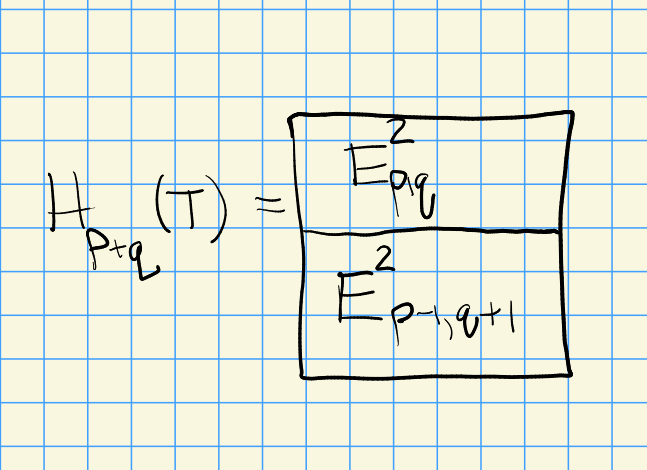
\includegraphics{figures/image_2021-03-15-09-29-09.png}
\caption{image\_2021-03-15-09-29-09}
\end{figure}

So in general, \(H_*(T)\) is determined up to extensions.

\end{exercise}

\begin{exercise}[5.1.2]

We view \(E^2_{*, *}\) as a 2nd order approximation to
\(H_*( {T}_{*} )\). We've used both differentials, so how do we
continue? There are well-defined maps
\(d_{p, q}^2: E_{p, q}^2 \to E^{2}_{p-2, q+1}\) such that
\(d^2_{*,*} \circ d^2_{*, *} = 0\) (noting that these are superscripts,
not squaring).

\end{exercise}

\begin{remark}

This yields differentials on \(E^2\) on lines of slope \(-1/2\) which
move from the \(n\)th diagonal to the \(n-1\)st diagonal:

\begin{center}
\begin{tikzcd}
    & {} & {} \\
    {q+1} && \bullet \\
    q &&&& \bullet \\
    \\
    && {p-2} && p & {} & {}
    \arrow["n"{pos=0}, color={rgb,255:red,92;green,214;blue,214}, dashed, no head, from=1-3, to=5-7]
    \arrow["{n-1}"{pos=0}, color={rgb,255:red,92;green,214;blue,214}, dashed, no head, from=1-2, to=5-6]
    \arrow[from=3-5, to=2-3]
\end{tikzcd}
\end{center}

\begin{quote}
\href{https://q.uiver.app/?q=WzAsMTAsWzIsNCwicC0yIl0sWzQsNCwicCJdLFswLDIsInEiXSxbMCwxLCJxKzEiXSxbMiwxLCJcXGJ1bGxldCJdLFs0LDIsIlxcYnVsbGV0Il0sWzIsMF0sWzYsNF0sWzEsMF0sWzUsNF0sWzYsNywibiIsMCx7ImxhYmVsX3Bvc2l0aW9uIjowLCJjb2xvdXIiOlsxODAsNjAsNjBdLCJzdHlsZSI6eyJib2R5Ijp7Im5hbWUiOiJkYXNoZWQifSwiaGVhZCI6eyJuYW1lIjoibm9uZSJ9fX0sWzE4MCw2MCw2MCwxXV0sWzgsOSwibi0xIiwwLHsibGFiZWxfcG9zaXRpb24iOjAsImNvbG91ciI6WzE4MCw2MCw2MF0sInN0eWxlIjp7ImJvZHkiOnsibmFtZSI6ImRhc2hlZCJ9LCJoZWFkIjp7Im5hbWUiOiJub25lIn19fSxbMTgwLDYwLDYwLDFdXSxbNSw0XV0=}{Link
to Diagram}
\end{quote}

\begin{center}
\begin{tikzcd}
    \bullet \\
    & \bullet & {(p, q)} \\
    && \bullet
    \arrow["{d^0}", from=2-3, to=3-3]
    \arrow["{d^2}"', from=2-3, to=1-1]
    \arrow["{d^1}", from=2-3, to=2-2]
\end{tikzcd}
\end{center}

\begin{quote}
\href{https://q.uiver.app/?q=WzAsNCxbMiwxLCIocCwgcSkiXSxbMiwyLCJcXGJ1bGxldCJdLFswLDAsIlxcYnVsbGV0Il0sWzEsMSwiXFxidWxsZXQiXSxbMCwxLCJkXjAiXSxbMCwyLCJkXjIiLDJdLFswLDMsImReMSJdXQ==}{Link
to Diagram}
\end{quote}

So we let \(E^3\) be the homology, and it turns out there are
differentials \(d^3: E^3_{p, q} \to E^3_{p-3, q+2}\) which go from
diagonal \(n\) to \(n-1\).

\end{remark}

\hypertarget{setup}{%
\subsection{Setup}\label{setup}}

\begin{definition}[Homology Spectral Sequences]

A \textbf{homology spectral sequence} starting with \(E^a\) for
\(a\in {\mathbb{Z}}\) in an abelian category \(\mathcal{A}\) consists of
the following data:

\begin{enumerate}
\def\labelenumi{\alph{enumi}.}
\item
  Pages: For all \(r\geq a\) and all \(p, q\in {\mathbb{Z}}\), a family
  \(\left\{{ E_{p, q}^r }\right\}\) of objects in \(\mathcal{A}\) (some
  of which my be zero), where typically \(a=1, 2\).
\item
  Differentials: A family of maps
  \(\left\{{ d_{p, q}^r: E_{p, q}^r \to E_{p-r, q+r-1}^r }\right\}\)
  with \(d^r \circ d^r =0\) of slope \(-\frac{r-1}{r}\) in that lattice
  \(E_{*, *}^r\) the form chain complexes. We take the convention that
  the differentials go to the left:
\end{enumerate}

\begin{center}
\begin{tikzcd}
    \bullet \\
    \\
    && \bullet \\
    \\
    &&&& \bullet
    \arrow["{d^r}", from=5-5, to=3-3]
    \arrow["{d^r}", from=3-3, to=1-1]
  \end{tikzcd}
\end{center}

\begin{quote}
\href{https://q.uiver.app/?q=WzAsMyxbNCw0LCJcXGJ1bGxldCJdLFsyLDIsIlxcYnVsbGV0Il0sWzAsMCwiXFxidWxsZXQiXSxbMCwxLCJkXnIiXSxbMSwyLCJkXnIiXV0=}{Link
to Diagram}
\end{quote}

\begin{enumerate}
\def\labelenumi{\alph{enumi}.}
\setcounter{enumi}{2}
\tightlist
\item
  Structure Maps: Isomorphisms
  \(E_{p, q}^{r+1} \cong \ker d_{p, q}^r / \operatorname{im}d_{p+r, q-r+1}^r\).
\end{enumerate}

We denote \(E^r_{*,*}\) to be the \textbf{\(r\)th page} of the sequence,
and the \textbf{total degree} of an entry \(E_{p, q}^r\) is \(p+q\).

\end{definition}

\begin{remark}

The term \(E_{p, q}^{r+1}\) is a \emph{subquotient}, i.e.~a submodule of
a quotient, of \(E_{p, q}^r\), and hence inductively a subquotient of
\(E_{p, q}^a\) by transitivity of ``being a subquotient''. The terms of
total degree \(n\) lie on a line of slope \(-1\), and each differential
\(d^r_{p, q}\) decreases the total degree by 1.

\end{remark}

\begin{remark}

There is a category of homology spectral sequences over a fixed abelian
category \(\mathcal{A}\). The objects consist of the above data of
pages, differentials, and structure maps from the above definition The
morphisms \(f: E\to \tilde E\) are families of maps
\begin{align*}
f_{p, q}^r: E_{p, q}^r \to \tilde{E}^r_{p, q}
\end{align*}
for all \(r \geq\max\left\{{a, \tilde a}\right\}\) with
\(\tilde{d}^r f^r = f^r d^r\) such that \(f_{p, q}^{r+1}\) is the map on
homology induced by \(f_{p, q}^r\).

\end{remark}

\begin{definition}[Cohomology Spectral Sequence]

A \textbf{cohomology} spectral sequence is defined dually: we'll write
this as \(E_r^{p, q}, d_r^{p, q}\), where the differentials go down and
to the right, and increase the total degree by 1:
\begin{align*}
d_r^{p, q}: E_r^{p, q} \to E_{r}^{p+r, q-r+1}
.\end{align*}

\begin{center}
\begin{tikzcd}
    q & \bullet \\
    \\
    {q-r+1} &&&&& \bullet \\
    & p &&&& {p+r}
    \arrow["{d_r^{p, q}}", from=1-2, to=3-6]
\end{tikzcd}
\end{center}

\begin{quote}
\href{https://q.uiver.app/?q=WzAsNixbMSwwLCJcXGJ1bGxldCJdLFs1LDIsIlxcYnVsbGV0Il0sWzEsMywicCJdLFs1LDMsInArciJdLFswLDAsInEiXSxbMCwyLCJxLXIrMSJdLFswLDEsImRfcl57cCwgcX0iXV0=}{Link
to Diagram}
\end{quote}

There is similarly a category of these.

\end{definition}

\begin{lemma}[Mapping Lemma]

Let \(f:E\to \tilde{E}\) be a morphism of spectral sequences (homology
or cohomology) such that for some fixed \(r\), the map
\(f^r: E_{p, q}^r\to \tilde{E}_{p, q}^r\) is an isomorphism for all
\(p, q\). Then all \(f^s_{p, q}\) are isomorphisms for all \(s\geq r\)
and all \(p, q\).

\end{lemma}

\begin{proof}[of the mapping lemma]

There is a commutative diagram with exact rows:

\begin{center}
\begin{tikzcd}
    0 && {B_{p, q}^r} && {Z_{p, q}^r} && {E_{p, q}^{r+1}} && 0 && 0 \\
    \\
    0 && {\tilde B_{p, q}^r} && {\tilde Z_{p, q}^r} && {\tilde E_{p, q}^r} && 0 && 0
    \arrow[from=1-1, to=1-3]
    \arrow[from=1-3, to=1-5]
    \arrow[from=1-5, to=1-7]
    \arrow[from=1-7, to=1-9]
    \arrow[from=3-1, to=3-3]
    \arrow[from=3-3, to=3-5]
    \arrow[from=3-5, to=3-7]
    \arrow[from=3-7, to=3-9]
    \arrow["{f_{p ,q}^r (\sim)}"', from=1-5, to=3-5]
    \arrow["{f_{p ,q}^r (\sim)}"', from=1-3, to=3-3]
    \arrow["{f_{p, q}^{r+1}}"', from=1-7, to=3-7]
    \arrow[from=1-9, to=1-11]
    \arrow[from=3-9, to=3-11]
    \arrow[no head, from=1-11, to=3-11]
    \arrow[no head, from=1-9, to=3-9]
\end{tikzcd}
\end{center}

\begin{quote}
\href{https://q.uiver.app/?q=WzAsMTIsWzAsMCwiMCJdLFsyLDAsIkJfe3AsIHF9XnIiXSxbNCwwLCJaX3twLCBxfV5yIl0sWzYsMCwiRV97cCwgcX1ee3IrMX0iXSxbOCwwLCIwIl0sWzIsMiwiXFx0aWxkZSBCX3twLCBxfV5yIl0sWzQsMiwiXFx0aWxkZSBaX3twLCBxfV5yIl0sWzYsMiwiXFx0aWxkZSBFX3twLCBxfV5yIl0sWzAsMiwiMCJdLFs4LDIsIjAiXSxbMTAsMCwiMCJdLFsxMCwyLCIwIl0sWzAsMV0sWzEsMl0sWzIsM10sWzMsNF0sWzgsNV0sWzUsNl0sWzYsN10sWzcsOV0sWzIsNiwiZl97cCAscX1eciAoXFxzaW0pIiwyXSxbMSw1LCJmX3twICxxfV5yIChcXHNpbSkiLDJdLFszLDcsImZfe3AsIHF9XntyKzF9IiwyXSxbNCwxMF0sWzksMTFdLFsxMCwxMSwiIiwxLHsic3R5bGUiOnsiaGVhZCI6eyJuYW1lIjoibm9uZSJ9fX1dLFs0LDksIiIsMSx7InN0eWxlIjp7ImhlYWQiOnsibmFtZSI6Im5vbmUifX19XV0=}{Link
to Diagram}
\end{quote}

Extending the right-hand side as indicate, we can apply the Five Lemma
to conclude that \(f_{p, q}^{r+1}\) is an isomorphism. Now do induction
on \(r\).

\end{proof}

\hypertarget{wednesday-march-17}{%
\section{Wednesday, March 17}\label{wednesday-march-17}}

\hypertarget{spectral-sequences}{%
\subsection{5.2: Spectral Sequences}\label{spectral-sequences}}

\begin{remark}

Recall that we had

\begin{itemize}
\tightlist
\item
  \(\left\{{ E_{p, q}^r {~\mathrel{\Big|}~}r\geq a, p,q\in {\mathbb{Z}}}\right\}\)
  for some \(a\).
\item
  \(d_{p, q}^r: E_{p, q}^r \to E_{p-r, q+r-1}\) with \(d^2=0\).
\item
  \(E_{p, q}^{r+1} \cong \ker d_{p, q}^r / \operatorname{im}d_{p+r,q-r+1}^r\).
\end{itemize}

\end{remark}

\begin{example}[First quadrant spectral sequences]

A \textbf{first quadrant} (homology) spectral sequence is one with
\(E_{p, q}^r = 0\) for \(p, q<0\). Note that for a fixed \(p, q\), there
is an \(r \gg 0\) such that the differential entering and leaving
\(E_{p, q}^r\) will be zero. The domain will be in quadrant 2 and the
codomain in quadrant 4. In this case \(E_{p, q}^r \cong E_{p, q}^{r+1}\)
and we call this ``stable'' module \(E_{p, q}^{\infty }\). Note that
\(r=r(p, q)\) can generally depend on \(p, q\).

\end{example}

\begin{definition}[Bounded]

We say a spectral sequence is \textbf{bounded} if there are only
finitely many nonzero terms of total degree \(n\). If so, there exists
some uniform \(r_0\) such that for \(r\geq r_0\), we have
\(E^{r}_{p, q} \cong E_{p, q}^{r+1} \cong E_{p, q}^{\infty }\).

\todo[inline]{See video for image.}

\end{definition}

\begin{remark}

For the rest of this course, we'll restrict our attention to bounded
spectral sequences.

\end{remark}

\begin{definition}[Convergence of a homology spectral sequences]

A bounded spectral sequences \(E\) \textbf{converges} to \(H_*\) if we
are given

\begin{enumerate}
\def\labelenumi{\arabic{enumi}.}
\item
  A family of objects \(\left\{{ H_n }\right\}_{n\in {\mathbb{Z}}}\)
\item
  For each \(n\), a finite (here increasing) filtration
  \begin{align*}
  0 = F_s H_n \subseteq \cdots \subseteq F_{p-1} H_n \subseteq F_p H_n \subseteq \cdots \subseteq F_t H_n = H_n
  \end{align*}
  where each \(F_i H_n\) is a subobject of \(H_n\)
\item
  Isomorphisms
  \begin{align*}
  E_{p, q}^{\infty } \cong { F_p H_{p +q} \over F_{p-1} H_{p+q}}
  ,\end{align*}
  or equivalently
  \begin{align*}
  E_{p, n-p}^{\infty } \cong { F_p H_n \over F_{p-1} H_n}
  ,\end{align*}
  which are the \(t-s\) \textbf{successive quotients} (or
  \textbf{sections}) of the filtration, which depend on \(n\). We refer
  to \(t-s\) as the \textbf{length} of the filtration
\end{enumerate}

In this case we write
\begin{align*}
E_{p, q}^a \Rightarrow H_{p+q}
,\end{align*}
thinking of \(a\to \infty\).

\end{definition}

\begin{remark}

We saw a case where the length of the filtration was 2, when we had
\(2\) columns. Recall that this only yields information up to
extensions, since this only computes quotients.

\end{remark}

\begin{remark}

We can form a similar definition for a cohomology spectral sequence. The
conditions change slightly:

(2') We have a \emph{decreasing} filtration
\begin{align*}
H^n = F^s H^n \supseteq \cdots \supseteq F^p H^n \supseteq F^{p+1} H^n \supseteq \cdots \supseteq F^t H^n = 0
.\end{align*}
In this case we have
\begin{align*}
E_{\infty }^{p, q} \cong {F^p H^{p+q} \over F^{p+1} H^{p+q} }
.\end{align*}
Then each \(H_n\) will have a filtration of length \(n+1\) by explicitly
counting terms on the diagonal, so we obtain
\begin{align*}
0 = F_{-1} H_n \subset F_0 H_n \subseteq \cdots \subseteq F_{n-1} H_n \subseteq F_n H_n = H_n
.\end{align*}

Then
\begin{align*}
E_{0, n} &\cong F_0 H_n \hookrightarrow H_n\\
E_{p, n-p} &\cong {F_p H_n \over F_{p-1} H_n} \\
H_n \twoheadrightarrow E_{n, 0} &\cong {H_n \over F_{n-1} H_n} 
.\end{align*}

\todo[inline]{See video for remarks!}

\end{remark}

\begin{definition}[Edge maps]

Assume that \(a\geq 1\). Provided \(a\geq 1\), note that \(E_{0, n}^r\)
is a quotient of \(E_{0, n}^a\) for all \(r\), since the outgoing (?)
differentials are all zero. Similarly, \(E_{n, 0}^r\) is a subobject of
\(E_{n, 0}^a\) for all \(r\). We thus have maps
\begin{align*}
E_{0, n}^a \twoheadrightarrow E_{0, n}^{\infty } \hookrightarrow H_n \\
H_n \twoheadrightarrow E_{n, 0}^{\infty } \hookrightarrow E_{n, 0}^a
.\end{align*}
These compositions are referred to as the \textbf{edge maps}.

\begin{figure}
\centering
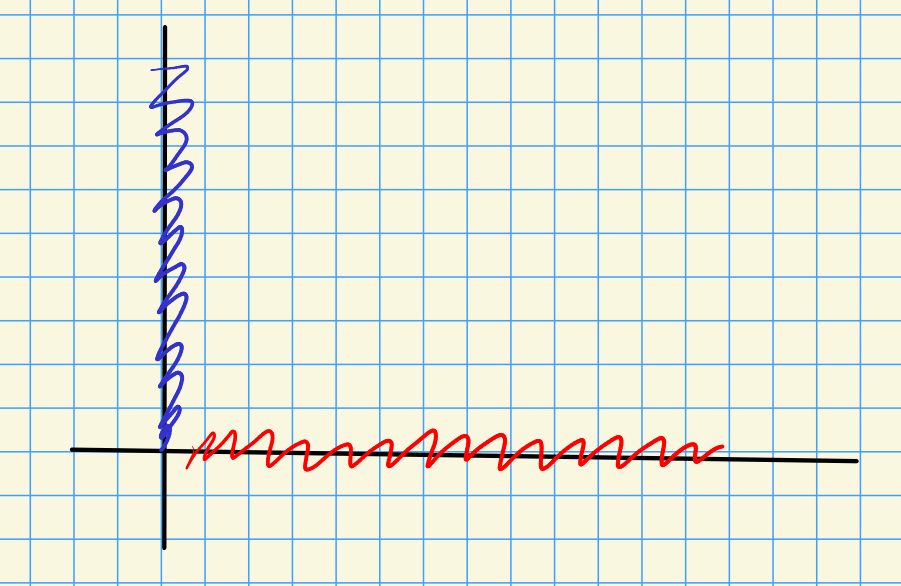
\includegraphics{figures/EdgeMaps.png}
\caption{Edges of a spectral sequence}
\end{figure}

\end{definition}

\begin{remark}

For a first quadrant \emph{cohomological} spectral sequence, the edge
maps are
\begin{align*}
E_{a}^{n, 0} \twoheadrightarrow E_{\infty }^{n, 0} \hookrightarrow H^n \\
H^n \twoheadrightarrow E_{\infty }^{0, n} \hookrightarrow E_{a}^{0, n}
.\end{align*}

\end{remark}

\begin{definition}[Collapsing of a spectral sequence]

A spectral sequence \(E\) \textbf{collapses} at \(E^r\) if there is
exactly one nonzero row (or column) in \(E_{*, *}^r\).

\end{definition}

\begin{remark}

This implies that \(E_{p, q}^r = E_{p, q}^{\infty }\) at this point. In
this case, we can read off the single nonzero section:

\begin{figure}
\centering
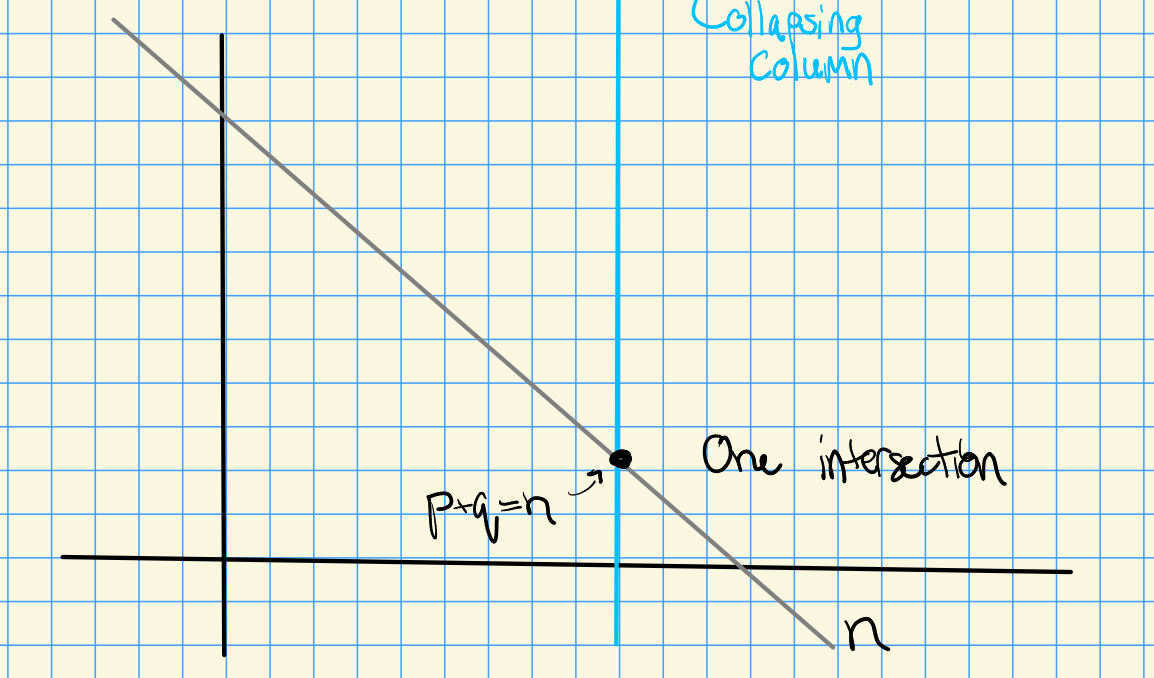
\includegraphics{figures/image_2021-03-17-09-55-34.png}
\caption{image\_2021-03-17-09-55-34}
\end{figure}

Here we'll have
\begin{align*}
E^{\infty }_{p, q} \cong {F_p H_n \over F_{p-1} H_n} \cong {H_n \over 0}\cong H_n
.\end{align*}

\end{remark}

\begin{remark}

A more common definition of a spectral sequence \textbf{collapsing at
\(r\)} is that for all \(p, q\), the differentials \(d_{p, q}^r = 0\).
Note that this implies stabilization at \(r\), but doesn't allow for
such a simple statement about the diagonals since they may intersect
multiple nonzero objects.

\end{remark}

\begin{remark}

Some things we're skipping from the book, around the last part of 5.2:

\begin{itemize}
\tightlist
\item
  Definitions pertaining to unbounded spectral sequences.
\item
  Weak convergence.
\item
  Filtrations that are infinite in on or both filtrations.
\item
  Filtrations that don't limit to a union equal to \(H_n\) or
  intersection to 0.
\item
  Abutment, which is convergence when the filtration is not finite.
\end{itemize}

We'll skip 5.3 on the Leray spectral sequence and jump to 5.4,
constructing a spectral sequence.

\end{remark}

\hypertarget{friday-march-19}{%
\section{Friday, March 19}\label{friday-march-19}}

\hypertarget{spectral-sequence-of-a-filtration}{%
\subsection{Spectral Sequence of a
Filtration}\label{spectral-sequence-of-a-filtration}}

\begin{definition}[?]

A \textbf{filtration} of a chain complex \(C\) is an ordered family of
subcomplexes
\begin{align*}
F\coloneqq& \cdots \subseteq F_{p-1}C \subseteq F_p C \subseteq \cdots \subseteq C && p\in {\mathbb{Z}}
\end{align*}
such that there are commutative diagrams

\begin{center}
\begin{tikzcd}
    {F_pC_n} && {C_n} \\
    \\
    {F_pC_{n-1}} && {C_{n-1}}
    \arrow["d", from=1-1, to=3-1]
    \arrow["d", from=1-3, to=3-3]
    \arrow[hook, from=1-1, to=1-3]
    \arrow[hook, from=3-1, to=3-3]
\end{tikzcd}
\end{center}

\begin{quote}
\href{https://q.uiver.app/?q=WzAsNCxbMCwwLCJGX3BDX24iXSxbMiwwLCJDX24iXSxbMCwyLCJGX3BDX3tuLTF9Il0sWzIsMiwiQ197bi0xfSJdLFswLDIsImQiXSxbMSwzLCJkIl0sWzAsMSwiIiwxLHsic3R5bGUiOnsidGFpbCI6eyJuYW1lIjoiaG9vayIsInNpZGUiOiJ0b3AifX19XSxbMiwzLCIiLDEseyJzdHlsZSI6eyJ0YWlsIjp7Im5hbWUiOiJob29rIiwic2lkZSI6InRvcCJ9fX1dXQ==}{Link
to Diagram}
\end{quote}

A filtration is \textbf{exhaustive} if
\(\bigcup_{p\in {\mathbb{Z}}} F_p C_n = C_n\) for all \(n\).

\end{definition}

\begin{remark}

The construction of the spectral sequence will show that \(C\) and
\(\bigcup_p F_p C\) give rise to the same spectral sequence. So we will
assume that all filtrations are exhaustive.

\end{remark}

\begin{theorem}[Construction of the spectral sequence of a filtration]

A filtration \(F\) of
\(C\in \mathsf{Ch}({\mathsf{R}{\hbox{-}}\mathsf{Mod}})\) determines a
spectral sequence starting with
\begin{align*}
E_{p, q}^0 { F_p C_{p+q} \over F_{p-1} C_{p+q} } && E_{p ,q}^1 = H_{p+q}(E^0_{p, *})
.\end{align*}

Since \(d\) preserves numerators and denominators, we get well-defined
differentials
\(\mkern 1.5mu\overline{\mkern-1.5mud\mkern-1.5mu}\mkern 1.5mu\) on the
quotients:

\begin{center}
\begin{tikzcd}
    &&&&& \textcolor{rgb,255:red,92;green,92;blue,214}{E_{p-1, q+1}^0} \\
    && {F_{p-1}C_{p+q+1}} & {} & {F_{p}C_{p+q+1}} && \textcolor{rgb,255:red,92;green,92;blue,214}{E_{p, q+1}^0} \\
    &&&&&&& \ddots \\
    \textcolor{rgb,255:red,92;green,92;blue,214}{F_{p-2}C_{p+q}} && \textcolor{rgb,255:red,92;green,92;blue,214}{F_{p-1}C_{p+q}} && {F_{p}C_{p+q}} && {E_{p, q}^0} \\
    \\
    && {F_{p-1}C_{p+q-1}} && {F_{p}C_{p+q-1}} && {E_{p, q-1}^0}
    \arrow[from=2-3, to=2-5]
    \arrow[from=2-5, to=2-7]
    \arrow[from=4-3, to=4-5]
    \arrow[from=4-5, to=4-7]
    \arrow[from=6-3, to=6-5]
    \arrow[from=6-5, to=6-7]
    \arrow["{\mkern 1.5mu\overline{\mkern-1.5mud\mkern-1.5mu}\mkern 1.5mu}"', from=2-7, to=4-7]
    \arrow["{\mkern 1.5mu\overline{\mkern-1.5mud\mkern-1.5mu}\mkern 1.5mu}"', from=4-7, to=6-7]
    \arrow["d"', from=2-5, to=4-5]
    \arrow["d"', from=4-5, to=6-5]
    \arrow["d"', from=2-3, to=4-3]
    \arrow["d"', from=4-3, to=6-3]
    \arrow[color={rgb,255:red,92;green,92;blue,214}, from=4-1, to=4-3]
    \arrow[color={rgb,255:red,92;green,92;blue,214}, from=1-6, to=2-7]
    \arrow[from=2-7, to=3-8]
\end{tikzcd}
\end{center}

\begin{quote}
\href{https://q.uiver.app/?q=WzAsMTMsWzIsMSwiRl97cC0xfUNfe3ArcSsxfSJdLFszLDFdLFsyLDMsIkZfe3AtMX1DX3twK3F9IixbMjQwLDYwLDYwLDFdXSxbMiw1LCJGX3twLTF9Q197cCtxLTF9Il0sWzQsMSwiRl97cH1DX3twK3ErMX0iXSxbNCwzLCJGX3twfUNfe3ArcX0iXSxbNCw1LCJGX3twfUNfe3ArcS0xfSJdLFs2LDEsIkVfe3AsIHErMX1eMCIsWzI0MCw2MCw2MCwxXV0sWzYsMywiRV97cCwgcX1eMCJdLFs2LDUsIkVfe3AsIHEtMX1eMCJdLFswLDMsIkZfe3AtMn1DX3twK3F9IixbMjQwLDYwLDYwLDFdXSxbNSwwLCJFX3twLTEsIHErMX1eMCIsWzI0MCw2MCw2MCwxXV0sWzcsMiwiXFxkZG90cyJdLFswLDRdLFs0LDddLFsyLDVdLFs1LDhdLFszLDZdLFs2LDldLFs3LDgsIlxcYmFye2R9IiwyXSxbOCw5LCJcXGJhcntkfSIsMl0sWzQsNSwiZCIsMl0sWzUsNiwiZCIsMl0sWzAsMiwiZCIsMl0sWzIsMywiZCIsMl0sWzEwLDIsIiIsMix7ImNvbG91ciI6WzI0MCw2MCw2MF19XSxbMTEsNywiIiwyLHsiY29sb3VyIjpbMjQwLDYwLDYwXX1dLFs3LDEyXV0=}{Link
to Diagram}
\end{quote}

Taking vertical homology of the \(E^0\) terms on the right yields
\(E_{p, q}^1\). Note that the blue terms contribute to the same diagonal
\(p+q=n\).

\end{theorem}

\begin{definition}[Bounded Filtrations]

A filtration \(F\) on a chain complex \(C\) is \textbf{bounded} if for
each \(n\) there are \(s<t\in {\mathbb{Z}}\) such that \(F_s C_n = 0\)
and \(F_t C_n = C_n\).

\end{definition}

\begin{remark}

Note that this implies that each diagonal of total degree \(n\) has only
finitely many nonzero terms, so the spectral sequence will again be
bounded. We'll next show that this spectral sequence converges to
\(H_*(C)\).

\end{remark}

\begin{definition}[Canonically Bounded Filtrations]

A filtration \(F\) is \textbf{canonically bounded} if and only if
\(F_{-1}C_n = 0\) and \(F_n C_n = C_n\) for all \(n\). In this case,
\begin{align*}
E_{p, q}^0 \coloneqq
{F_p C_{p+q} \over F_{p-1} C_{p+q}} = 
\begin{cases}
0 & p < 0  
\\
0 & q < 0 \quad (p>n, p-1\geq n).
\end{cases}
\end{align*}

So \(E\) becomes a first quadrant spectral sequence.

\end{definition}

\begin{remark}

Note that all elements on all pages are subquotients of \(E^0\)
elements, so they can only get smaller, and terms that become 0 on some
page stay 0 for all remaining pages.

\end{remark}

\hypertarget{construction-of-the-spectral-sequence-of-a-filtration}{%
\subsection{Construction of the Spectral Sequence of a
Filtration}\label{construction-of-the-spectral-sequence-of-a-filtration}}

\begin{remark}

For ease of notation, we'll suppress the subscript \(q\) since it can
always be recovered as \(q = n-p\). Define the canonical quotients
\begin{align*}
\eta_p: F_p C \to F_p C / F_{p-1}C = E_p^0
.\end{align*}

Define
\begin{align*}
A^r_p \coloneqq\left\{{ c\in F_p C {~\mathrel{\Big|}~}d(c) \in F_{p-r}(C) }\right\} 
,\end{align*}
which are elements of \(F_p C\) which are cycles modulo \(F_{p-r} C\),
the \textbf{approximate cycles}. Note that any actual cycle is in all
\(A^r\). This differential takes things \(r\) columns to the left, so
we'll want to define a differential that associates the following terms

\begin{center}
\begin{tikzcd}
    &&& {F_{p-1}C_{n+1}} & {} & {F_{p}C_{n+1}} \\
    \\
    &&& \textcolor{rgb,255:red,153;green,92;blue,214}{F_{p-1}C_{n}} && {F_{p}C_{n}} & c \\
    \\
    \textcolor{rgb,255:red,153;green,92;blue,214}{F_{p-r}C} & \cdots && {F_{p-1}C_{n-1}} && {F_{p}C_{n-1}} & dc
    \arrow[hook, from=1-4, to=1-6]
    \arrow[hook, from=3-4, to=3-6]
    \arrow[hook, from=5-4, to=5-6]
    \arrow["d"', from=1-6, to=3-6]
    \arrow["d"', from=3-6, to=5-6]
    \arrow["d"', from=1-4, to=3-4]
    \arrow["d"', from=3-4, to=5-4]
    \arrow[hook, from=5-1, to=5-2]
    \arrow[maps to, from=3-7, to=5-7]
\end{tikzcd}
\end{center}

\begin{quote}
\href{https://q.uiver.app/?q=WzAsMTEsWzMsMCwiRl97cC0xfUNfe24rMX0iXSxbNCwwXSxbMywyLCJGX3twLTF9Q197bn0iLFsyNzAsNjAsNjAsMV1dLFszLDQsIkZfe3AtMX1DX3tuLTF9Il0sWzUsMCwiRl97cH1DX3tuKzF9Il0sWzUsMiwiRl97cH1DX3tufSJdLFs1LDQsIkZfe3B9Q197bi0xfSJdLFswLDQsIkZfe3Atcn1DIixbMjcwLDYwLDYwLDFdXSxbMSw0LCJcXGNkb3RzIl0sWzYsMiwiYyJdLFs2LDQsImRjIl0sWzAsNCwiIiwwLHsic3R5bGUiOnsidGFpbCI6eyJuYW1lIjoiaG9vayIsInNpZGUiOiJ0b3AifX19XSxbMiw1LCIiLDAseyJzdHlsZSI6eyJ0YWlsIjp7Im5hbWUiOiJob29rIiwic2lkZSI6InRvcCJ9fX1dLFszLDYsIiIsMCx7InN0eWxlIjp7InRhaWwiOnsibmFtZSI6Imhvb2siLCJzaWRlIjoidG9wIn19fV0sWzQsNSwiZCIsMl0sWzUsNiwiZCIsMl0sWzAsMiwiZCIsMl0sWzIsMywiZCIsMl0sWzcsOCwiIiwyLHsic3R5bGUiOnsidGFpbCI6eyJuYW1lIjoiaG9vayIsInNpZGUiOiJ0b3AifX19XSxbOSwxMCwiIiwwLHsic3R5bGUiOnsidGFpbCI6eyJuYW1lIjoibWFwcyB0byJ9fX1dXQ==}{Link
to Diagram}
\end{quote}

Similarly, define
\begin{align*}
Z_p^r &\coloneqq\eta_p(A_p^r \subseteq E_p^0 \\
B_p^r &\coloneqq\eta_p(d A_{p+r-1}^{r-1}) \subseteq \eta_p(F_p C) \subseteq E_p^0 
.\end{align*}

\end{remark}

\begin{observation}

Some key observations:

\begin{enumerate}
\def\labelenumi{\arabic{enumi}.}
\item
  \(F_p C = A_p^0 = A_p^{-1} = A_p^{-2} = \cdots\)
\item
  \(A_p^{r+1} \subseteq A_p^r\)
\item
  \(A_p^r \cap F_{p-1} C = A_{p-1}^{r-1}\).
\end{enumerate}

\end{observation}

\begin{exercise}[?]

Work through these facts using the diagram above.

\end{exercise}

\begin{remark}

Some consequences:

\((1) \implies Z_p^0 = E_p^0\) (taking \(r=0\) in the quotient map
\(\eta_p\)).

\((2) \implies Z_p^{r+q} \subseteq Z_p^r\), since these are images of
subgroups

\((3) \implies A_{p+r-1}^{r-1} \subseteq A_{p+r}^r\), replacing
\(p\mapsto p+r\) in the intersection formula. Then applying \(d\) yields
\(B_p^r \subseteq D_p^{r+1}\).

\((1) \implies B_p^0 = \eta_p(d A_{p-1}^{-1}) \subseteq \eta_p(F_{p-1} C) = 0\),
since this occurs in the denominator for \(\eta_p\) and \(d\) preserves
filtration degree.

So the \(Z_p\) get smaller and the \(B_p\) get bigger. What happens in
the middle?

\end{remark}

\begin{proposition}[All boundaries are contained in all cycles in a spectral sequence]

\(B_p^r \subseteq Z_p^s\) for all \(r, s\geq 0\).

\end{proposition}

\begin{proof}[?]

A sequence of implications:
\begin{align*}
B_p^r \ni x = \eta_p(dc) \text{ for some }c 
&\implies d(dc) = 0 \in F_{p-s}C \, \forall s \\
&\implies dc \in A_p^s \\
&\implies \eta_p(dc) \in Z_p^s
.\end{align*}

\end{proof}

\begin{remark}

Set
\(B_p^{\infty } \coloneqq\cup_{r\geq 1} B_p^r \subseteq Z_p^{\infty } \coloneqq\bigcap_{s\geq 1} Z_p^s\),
which follows from a set theory exercise.

\end{remark}

\begin{remark}

Combining and summarizing these results: for every \(p\geq 0\), we have
a tower of groups:

\begin{center}
\begin{tikzcd}
    {0 = B_p^0} & {B_p^1} & \cdots & {B_p^r} & \cdots & {B_p^\infty} & {Z_p^{\infty}} & \cdots & {Z_p^{r}} & \cdots & {Z_p^{1}} & {Z_p^{0} = E_p^0}
    \arrow[hook, from=1-1, to=1-2]
    \arrow[hook, from=1-2, to=1-3]
    \arrow[hook, from=1-3, to=1-4]
    \arrow[hook, from=1-4, to=1-5]
    \arrow[hook, from=1-5, to=1-6]
    \arrow[hook, from=1-6, to=1-7]
    \arrow[hook, from=1-7, to=1-8]
    \arrow[hook, from=1-8, to=1-9]
    \arrow[hook, from=1-9, to=1-10]
    \arrow[hook, from=1-10, to=1-11]
    \arrow[hook, from=1-11, to=1-12]
\end{tikzcd}
\end{center}

\begin{quote}
\href{https://q.uiver.app/?q=WzAsMTIsWzAsMCwiMCA9IEJfcF4wIl0sWzEsMCwiQl9wXjEiXSxbMywwLCJCX3BeciJdLFs1LDAsIkJfcF5cXGluZnR5Il0sWzIsMCwiXFxjZG90cyJdLFs0LDAsIlxcY2RvdHMiXSxbNiwwLCJaX3Bee1xcaW5mdHl9Il0sWzgsMCwiWl9wXntyfSJdLFsxMCwwLCJaX3BeezF9Il0sWzExLDAsIlpfcF57MH0gPSBFX3BeMCJdLFs3LDAsIlxcY2RvdHMiXSxbOSwwLCJcXGNkb3RzIl0sWzAsMSwiIiwwLHsic3R5bGUiOnsidGFpbCI6eyJuYW1lIjoiaG9vayIsInNpZGUiOiJ0b3AifX19XSxbMSw0LCIiLDAseyJzdHlsZSI6eyJ0YWlsIjp7Im5hbWUiOiJob29rIiwic2lkZSI6InRvcCJ9fX1dLFs0LDIsIiIsMCx7InN0eWxlIjp7InRhaWwiOnsibmFtZSI6Imhvb2siLCJzaWRlIjoidG9wIn19fV0sWzIsNSwiIiwwLHsic3R5bGUiOnsidGFpbCI6eyJuYW1lIjoiaG9vayIsInNpZGUiOiJ0b3AifX19XSxbNSwzLCIiLDAseyJzdHlsZSI6eyJ0YWlsIjp7Im5hbWUiOiJob29rIiwic2lkZSI6InRvcCJ9fX1dLFszLDYsIiIsMCx7InN0eWxlIjp7InRhaWwiOnsibmFtZSI6Imhvb2siLCJzaWRlIjoidG9wIn19fV0sWzYsMTAsIiIsMCx7InN0eWxlIjp7InRhaWwiOnsibmFtZSI6Imhvb2siLCJzaWRlIjoidG9wIn19fV0sWzEwLDcsIiIsMCx7InN0eWxlIjp7InRhaWwiOnsibmFtZSI6Imhvb2siLCJzaWRlIjoidG9wIn19fV0sWzcsMTEsIiIsMCx7InN0eWxlIjp7InRhaWwiOnsibmFtZSI6Imhvb2siLCJzaWRlIjoidG9wIn19fV0sWzExLDgsIiIsMCx7InN0eWxlIjp7InRhaWwiOnsibmFtZSI6Imhvb2siLCJzaWRlIjoidG9wIn19fV0sWzgsOSwiIiwwLHsic3R5bGUiOnsidGFpbCI6eyJuYW1lIjoiaG9vayIsInNpZGUiOiJ0b3AifX19XV0=}{Link
to Diagram}
\end{quote}

\end{remark}

\begin{remark}

Note that using standard isomorphism theorems, we have
\begin{align*}
Z_p^r \cong {A_p^r \over A_p^r \cap F_{p-1}C C} \overset{(3)}{=} {A_p^r \over A_{p-1}^{r-1}}
.\end{align*}
So set
\begin{align*}
E_p^r \coloneqq Z_p^r/B_p^r \cong {A_p^r + F_{p-1} C \over d A_{p+r-1}^{r-1} + F_{p-1}C } \cong {A_p^r \over d A_{p+r-q}^{r-1} + A_{p-1}^{r-1}}
,\end{align*}
making \(E_p^r\) a quotient of \(A_p^r\). Using a similar calculation,
one can show
\begin{align*}
{Z_p^{r+1} \over B_p^r} 
\cong 
{ A_p^{r+1} + A_{p-1}^{r-1} \over dA_{p+r-1}^{r-1} + A_{p-1}^{r-1} }
.\end{align*}

\end{remark}

\begin{remark}

There will be an induced differential on this quotient, which will
follow from checking that the different preserves the numerator and
denominator.

\end{remark}

\hypertarget{monday-march-22}{%
\section{Monday, March 22}\label{monday-march-22}}

\hypertarget{spectral-sequence-of-a-filtration-1}{%
\subsection{5.4: Spectral Sequence of a
Filtration}\label{spectral-sequence-of-a-filtration-1}}

\begin{remark}

We have an increasing filtration \(F_p C \subseteq F_{p+1}C\), where we
defined
\begin{align*}
E_{p, q}^0 = { F_p C_{p+q} \over F_{p-1} C_{p+1} } &&
E_{p,q}^1 = H_{p+q} E_{p, *}^0
.\end{align*}

\begin{enumerate}
\def\labelenumi{\arabic{enumi}.}
\item
  We have a map
  \begin{align*}
    \eta_p: F_p C \twoheadrightarrow{F_p C \over F_{p-1}C } = E_p^0
    ,\end{align*}
  where we've dropped the \(q\) from notation.
\item

  \begin{align*}
    A_{p, q}^r = \left\{{ c \in C_p C {~\mathrel{\Big|}~}dc \in F_{p-1} C }\right\} 
    ,\end{align*}
  the eventual cycles. We defined \(Z_p^r = \eta_p A_p^r\) and
  \(B_p^r = \eta_p dA_{p+r-1}^{r-1}\), and wrote
  \(A_p^r \cap F_{p-1}C = A_{p-1}^{r-1}\).
\item
  We had the chain of inclusions
  \begin{align*}
  0 = B_p^r \subseteq \cdots \subseteq B_p^{\infty} \subset Z_p^{\infty } \subset \cdots \subseteq Z_p^1 = E_p^)
  .\end{align*}
\item
  We also have
  \(E_p^r = Z_p^r/B_p^r = A_p^r / dA_{p+r-1}^{r-1} + A_{p-1}^{r-1}\)
\item
  \(Z_{p}^{r+1}/B_pr \cong {A_p^{r+1} +A_{p-1}^{r-1} \over dA_{p+r-1} ^{r-1} + A_{p-1}^{r-1}}\).
\item
  \(dA_p^r \cap F_{p-r-1} C = dA_P^{r+1}\).
\end{enumerate}

\todo[inline]{See video for missed spoken details!}

Obviously we have
\begin{align*}
d: A_p^r &\to A_{p-r}^{r} \\
d: A_{p-1}^r &\to dA_{p-1}^{r-1} 
,\end{align*}
so \(d\) induces a well-defined map
\(d_p^r: E_p^r \xrightarrow{} E_{p-r}^r\), which of course squares to
zero, which goes \(r\) columns to the left and decreases the total
degree \(n\) by 1 since the original \(d\) did on \(C_n\). This is what
we need to set up a spectral sequence, since we now have pages and
differentials, and it just remains to show that
\(E^{r+1} \cong H_*(E^r, d^r)\).

\end{remark}

\begin{lemma}[?]

\(d\) determines isomorphisms
\(Z_{p}^r/Z_p^{r+1} \xrightarrow{\sim} B_{p-r}^{r+1} / B_{p-r}^r\).

\end{lemma}

\begin{proof}[?]

Unwind definitions! Note that we have
\(B_{p-r}^{r+1} = \eta_{p-r} dA_p^r\), using that the lower index on
\(B\) and upper index on \(A\) should sum to the lower index on \(A\).
This is equal to \(dA_p^r / dA_p^r \cap F_{p-r-1} C\), where the latter
term is \(\ker\eta_{p-r}\) and
\(B_{p-r}^r = \eta_{p-r} dA_{p-1}^{r-1}\). This yields
\begin{align*}
{B^{r+1}_{p-r} \over B_{p-r}^r}  
\cong 
{ dA_{p}^r \over dA_{p-1}^{r-1} + (dA_p^r \cap F_{p-r-1} C) }
.\end{align*}
Similarly,
\begin{align*}
{Z_p^r \over Z_p^{r+1}} \coloneqq{ \eta_p A_p^r \over \eta_p A_p^{r+1} } \cong {A_p^r \over A_p^{r+1} + (A_p^r \cap F_{p-1} C )}
\overset{(3)}{\cong} {A_p^r \over A_p^{r+1} + A_{p-1}^{r-1} }
.\end{align*}
Now applying the map induced by \(d: A_p^r \to F_{p-r}C\) to this
quotient, we have
\(\ker { \left.{{d}} \right|_{{A_p^r}} } \subseteq A_p^{r+1}\). These go
down \(r\) steps, but everything in the kernel goes down as far as you'd
like! So \(d\) kills one of the denominator terms, and thus induces an
injective map on the quotient. Thus
\({Z_p^r \over Z_p^{r+1}} \xrightarrow{\sim} {dA_p^r \over dA_p^{r+1} + dA_{p-1}^{r-1} }\),
which is exactly the previous expression with the order switched, so
this is isomorphic to \(B_{p-r}^{r+1} / B_{p-r}^r\).

\end{proof}

\begin{proposition}[The $r+1$st page is the homology of the $r$th page]

\begin{align*}
{ \ker d_p^r \over \operatorname{im}d_{p+r}^r } \cong E_p^{r+1} \coloneqq{Z_p^{r+1} \over B_p^{r+1} }
.\end{align*}

\end{proposition}

\begin{proof}[?]

Recall that \(d_p^r: E_p^r \to E_{p-r}^r\) and by (4),
\(E_p^r \cong {A_p^r \over dA_{p+r-1}^{r-1} + A_{p-1}^{r-1}}\).
Substituting \(p \mapsfrom p-r\), we have
\begin{align*}
\ker d_p^r = 
{
\left\{{ z\in A_p^r {~\mathrel{\Big|}~}dz \in dA_{p-1}^{r-1} + A_{p-r-1}^{r-1} }\right\} 
\over
dA_{p+r-1}^{r-1} + A_{p-1}^{r-1}
}
=
{
A_{p-1}^{r-1} + A_{p}^{r+1}
\over 
dA_{p+r-1}^{r-1} + A_{p-1}^{r-1}
}
\overset{(5)}{\cong}
{Z_p^{r+1} \over B_p^r} && \text{which is } (6)
.\end{align*}
Here we've used that
\(x\in F_p C\implies dx \in F_{p-r-1} C \implies dx\in A^{?}_{p-r-1}\).
What is the image of \(d_p^r\) in general? Note that later we can
replace \(p\mapsfrom p+r\). By the 1st isomorphism theorem, we have
\begin{align*}
d_p^r: E_p^r = Z_p^r / B_p^r \xrightarrow{\sim} {Z_p^r / B_p^r \over Z_p^{r+1} / B_p^r} \xrightarrow{\sim} {Z_p^r \over Z_p^{r+1}} \xrightarrow{d} 
{B_{p-r}^{r+1} \over B_{p-r}^r} \hookrightarrow{Z_{p-r}^r \over B_{p-r}^r} = E_{p-r}^r
,\end{align*}
where we've applied the lemma from last time, and we've used the fact
that in the last map, all of the \(B\) are contained in all of the
\(Z\), so we can choose any superscript we want. These are all
isomorphisms up until the last part, so
\begin{align*}
\operatorname{im}d_p^r \cong B_{p-r}^{r+1} / B_{p-r}^{r+1}
.\end{align*}
. Replacing \(p\mapsfrom p+r\), we get a 7th fact

\begin{fact}[7]

\begin{align*}
\operatorname{im}d_{p+r}^r \cong B_{p}^{r+1} / B_{p}^{r+1}
.\end{align*}

\end{fact}

Now combining (6) and (7), we have
\begin{align*}
{\ker d_p^r \over \operatorname{im}d_{p+r}^{r} } \xrightarrow{\sim} {Z_p^{r+1} / B_p^r \over B_{p}^{r+1} / B_p^r } \cong {Z_p^{r+1} \over B_p^{r+1}} = E_p^{r+1}
.\end{align*}

\end{proof}

\hypertarget{convergence-of-the-spectral-sequence-of-a-filtration}{%
\subsection{5.5: Convergence of the Spectral Sequence of a
Filtration}\label{convergence-of-the-spectral-sequence-of-a-filtration}}

\begin{remark}

We'll restrict our attention to bounded complexes.

\end{remark}

\begin{remark}

A filtration \(F\) on a chain complex \(C\) induces a filtration on the
homology \(H_*C\), where
\(H_p H_n C = \operatorname{im}( H_n F_p C \to H_n C)\):

\begin{center}
\begin{tikzcd}
    {F_p C_{n+1}} && {C_{n+1}} \\
    \\
    {F_p C_{n}} && {C_{n}} \\
    \\
    {F_p C_{n-1}} && {C_{n-1}}
    \arrow[hook, from=1-1, to=1-3]
    \arrow[hook, from=3-1, to=3-3]
    \arrow[hook, from=5-1, to=5-3]
    \arrow["d"{description}, from=1-1, to=3-1]
    \arrow["d"{description}, from=3-1, to=5-1]
    \arrow["d"{description}, from=1-3, to=3-3]
    \arrow["d"{description}, from=3-3, to=5-3]
\end{tikzcd}
\end{center}

\begin{quote}
\href{https://q.uiver.app/?q=WzAsNixbMCwwLCJGX3AgQ197bisxfSJdLFsyLDAsIkNfe24rMX0iXSxbMiwyLCJDX3tufSJdLFsyLDQsIkNfe24tMX0iXSxbMCwyLCJGX3AgQ197bn0iXSxbMCw0LCJGX3AgQ197bi0xfSJdLFswLDEsIiIsMCx7InN0eWxlIjp7InRhaWwiOnsibmFtZSI6Imhvb2siLCJzaWRlIjoidG9wIn19fV0sWzQsMiwiIiwwLHsic3R5bGUiOnsidGFpbCI6eyJuYW1lIjoiaG9vayIsInNpZGUiOiJ0b3AifX19XSxbNSwzLCIiLDAseyJzdHlsZSI6eyJ0YWlsIjp7Im5hbWUiOiJob29rIiwic2lkZSI6InRvcCJ9fX1dLFswLDQsImQiLDFdLFs0LDUsImQiLDFdLFsxLDIsImQiLDFdLFsyLDMsImQiLDFdXQ==}{Link
to Diagram}
\end{quote}

\todo[inline]{See video for missed details.}

These inclusions induce a map from the homology of the subcomplex to the
homology of the total complex.

\end{remark}

\begin{remark}

If the filtration on \(C\) is bounded, say
\(0 = F_s C_n \subseteq \cdots \subseteq F_t C_n = C_n\) for some
\(s<t\), then so is the induced filtration on \(H_n C\). Also note that
\(F_t H_n = H_n\) and \(F_s H_n = 0\).

\end{remark}

\begin{theorem}[Classical Convergence Theorem]

Assume \(F\) is a bounded filtration on \(C\), then the spectral
sequence is bounded and converges to \(H_*C\), so
\begin{align*}
E^1_{p, q} = H_{p+q}\qty{ F_p C \over F_{p-1} C } \Rightarrow H_{p+q}C
.\end{align*}

\end{theorem}

\begin{remark}

Need to check next time that the \(E^{\infty }_{p, q}\) terms give the
proper quotients.

\end{remark}

\hypertarget{wednesday-march-24}{%
\section{Wednesday, March 24}\label{wednesday-march-24}}

\begin{remark}

Last time: we're trying to prove the classical convergence theorem in
the bounded case. We have
\begin{align*}
E_{pq}^1 = H_{p+q}( F_p C/ F_{p-1} C ) \Rightarrow H_{p+q}C
.\end{align*}
We'd like this converge, i.e.~the \(E^\infty\) page will be the sections
of \(H_{p+q}C\). Writing \(C_n'\coloneqq F_p C_n\) for the filtered
pieces, we have

\begin{center}
\begin{tikzcd}
    {C_n'} && {C_n} \\
    {Z_n'} && {Z_n} \\
    {B_n'} && {B_n}
    \arrow[hook, from=3-1, to=3-3]
    \arrow[hook, from=2-1, to=2-3]
    \arrow[hook, from=1-1, to=1-3]
    \arrow[hook, from=1-3, to=2-3]
    \arrow[hook, from=2-3, to=3-3]
    \arrow[hook, from=1-1, to=2-1]
    \arrow[hook, from=2-1, to=3-1]
\end{tikzcd}
\end{center}

\begin{quote}
\href{https://q.uiver.app/?q=WzAsNixbMCwwLCJDX24nIl0sWzIsMCwiQ19uIl0sWzAsMSwiWl9uJyJdLFsyLDEsIlpfbiJdLFswLDIsIkJfbiciXSxbMiwyLCJCX24iXSxbNCw1LCIiLDAseyJzdHlsZSI6eyJ0YWlsIjp7Im5hbWUiOiJob29rIiwic2lkZSI6InRvcCJ9fX1dLFsyLDMsIiIsMCx7InN0eWxlIjp7InRhaWwiOnsibmFtZSI6Imhvb2siLCJzaWRlIjoidG9wIn19fV0sWzAsMSwiIiwwLHsic3R5bGUiOnsidGFpbCI6eyJuYW1lIjoiaG9vayIsInNpZGUiOiJ0b3AifX19XSxbMSwzLCIiLDEseyJzdHlsZSI6eyJ0YWlsIjp7Im5hbWUiOiJob29rIiwic2lkZSI6InRvcCJ9fX1dLFszLDUsIiIsMSx7InN0eWxlIjp7InRhaWwiOnsibmFtZSI6Imhvb2siLCJzaWRlIjoidG9wIn19fV0sWzAsMiwiIiwxLHsic3R5bGUiOnsidGFpbCI6eyJuYW1lIjoiaG9vayIsInNpZGUiOiJ0b3AifX19XSxbMiw0LCIiLDEseyJzdHlsZSI6eyJ0YWlsIjp7Im5hbWUiOiJob29rIiwic2lkZSI6InRvcCJ9fX1dXQ==}{Link
to Diagram}
\end{quote}

Then the induced filtration on homology is
\begin{align*}
H_n' \coloneqq{Z_n' \over B_n'} &\hookrightarrow H_n \coloneqq{Z_n\over B_n} \\
z' + B_n' &\mapsto z' + B_n
.\end{align*}

\end{remark}

\begin{proof}[of classical convergence theorem]

As discussed, we have a natural bounded filtration on each \(H_n C\).
Fixing \(p, n\) and writing \(q = n-p\), we have
\begin{align*}
A_p^r = \left\{{ c \in F_p C_n {~\mathrel{\Big|}~}d(c) \in F_{p-r} C_{n-1} }\right\} 
.\end{align*}
This stabilizes for large \(r\), namely whenever \(F_{p-r} C_{n-1} = 0\)
(which happens since the complex is bounded). Call the stabilized object
\(A_p^{\infty } \coloneqq\left\{{ c\in F_p C_n {~\mathrel{\Big|}~}d(c) = 0 }\right\}\),
which is \(\ker d\) in the \(p\)th filtered piece. Some facts:

\begin{enumerate}
\def\labelenumi{\arabic{enumi}.}
\setcounter{enumi}{-1}
\item
  \(Z_p^r = \eta_p(A_p^r)\) where
  \begin{align*}
  \eta_p: F_p C_n \to {F_p C_n \over F_{p-1} C_n }
  \end{align*}
  where \(Z_p^{\infty } = \eta_p(A_p^{\infty })\).
\item
  \(A_p^{\infty } \coloneqq\ker (F_p C_n \xrightarrow{d} F_p C_{n-1} )\),
  which is the ``numerator'' of \(F_p H_n C\).
\item
  \(d(C_{n+1}) \cap F_p C_n = \bigcup_{r\in {\mathbb{Z}}} d(A_{p+r}^r )\):

  \begin{center}
  \begin{tikzcd}
   &&&& {A_{p+r}} \\
   &&&& {F_{p+r}C_{n+1}} & {C_{n+1}} \\
   {F_p C_n}
   \arrow["d"', from=1-5, to=3-1]
   \arrow[hook, from=1-5, to=2-5]
   \arrow[hook, from=2-5, to=2-6]
    \end{tikzcd}
  \end{center}
\end{enumerate}

\begin{quote}
\href{https://q.uiver.app/?q=WzAsNCxbNCwwLCJBX3twK3J9Il0sWzQsMSwiRl97cCtyfUNfe24rMX0iXSxbNSwxLCJDX3tuKzF9Il0sWzAsMiwiRl9wIENfbiJdLFswLDMsImQiLDJdLFswLDEsIiIsMix7InN0eWxlIjp7InRhaWwiOnsibmFtZSI6Imhvb2siLCJzaWRlIjoidG9wIn19fV0sWzEsMiwiIiwyLHsic3R5bGUiOnsidGFpbCI6eyJuYW1lIjoiaG9vayIsInNpZGUiOiJ0b3AifX19XV0=}{Link
to Diagram}
\end{quote}

\begin{enumerate}
\def\labelenumi{\arabic{enumi}.}
\setcounter{enumi}{2}
\item
  Recall that we defined \(B_p^r \coloneqq\eta_p( d A_{p+r-1}^{r-1} )\).
  We can write \(B_p^{\infty } = \eta_p (\cup_r dA_{p+r}^r )\), where
  the left-hand side and the inner term on the right-hand side are equal
  to \(\bigcup_{r\geq 1} B_p^r\).
\item
  \(A_{p-1}^{\infty } = A_p^{\infty } \cap F_{p-1} C_n = \ker (A_{p}^{\infty } \xrightarrow{\eta_p} E_p^0 )\).
\end{enumerate}

Now to assemble this, note that
\begin{align*}
{F_p H_n C \over F_{p-1} H_n C} 
&\cong 
{A_{p}^{\infty } \over A_{p-1}^{\infty } + \bigcup_r dA_{p+r}^r } 
&& \text{ by 1 and 2} \\
&\cong
{ \eta_p (A_p^{\infty } ) \over \eta_p\qty{\bigcup_{r\geq 0} dA_{p+r}^r } } 
&& \text{by 4} \\
&= {Z_p^{\infty } \over B_p^{\infty } } 
&& \text{by 0, 3} \\
&= E_p^{\infty }
.\end{align*}
where we've used that
\(A_{p-1}^{\infty } + \bigcup_{r>0} dA_{p+r}^r \subseteq \ker \eta_p = F_{p-1} C\).

\end{proof}

\hypertarget{applications-two-spectral-sequences-of-a-double-complex}{%
\subsection{Applications: Two Spectral Sequences of a Double
Complex}\label{applications-two-spectral-sequences-of-a-double-complex}}

\begin{remark}

Consider two different filtrations of the total complex
\(\operatorname{Tot}(C)\) (either sum or product) of a double complex
\(C_{*, *}\). We know there is an spectral sequence associated to each
and play them off of each other to get extra information about
cohomology.

\end{remark}

\begin{definition}[Filtration I: by columns (of a double complex)]

Let \({}^IF_n \operatorname{Tot}(C)\) be the total subcomplex obtain by
applying truncation functors:
\begin{align*}
\qty{{}^I \tau_{\leq n} C}_{p, q} \coloneqq
\begin{cases}
C_{p, q} & p \leq n 
\\
0 & p > n.
\end{cases}
.\end{align*}

\begin{center}
\begin{tikzcd}
    \ddots & \vdots & \vdots & {} & \vdots & \vdots \\
    \cdots & \bullet & \bullet && 0 & 0 & \cdots \\
    \cdots & \bullet & \bullet && 0 & 0 & \cdots \\
    \cdots & \bullet & \bullet && 0 & 0 & \cdots \\
    \bullet & \vdots & \vdots & {} & \vdots & \vdots & \bullet \\
    && n & \bullet & {n+1}
    \arrow[no head, from=5-1, to=5-7]
    \arrow[no head, from=1-4, to=6-4]
    \arrow[from=2-3, to=2-2]
    \arrow[from=2-3, to=3-3]
    \arrow[from=3-3, to=3-2]
    \arrow[from=3-3, to=4-3]
    \arrow[from=4-3, to=4-2]
    \arrow[color={rgb,255:red,92;green,92;blue,214}, dotted, no head, from=1-1, to=5-5]
\end{tikzcd}
\end{center}

\begin{quote}
\href{https://q.uiver.app/?q=WzAsMzQsWzIsMSwiXFxidWxsZXQiXSxbMiwyLCJcXGJ1bGxldCJdLFsxLDIsIlxcYnVsbGV0Il0sWzEsMSwiXFxidWxsZXQiXSxbMSwzLCJcXGJ1bGxldCJdLFsyLDMsIlxcYnVsbGV0Il0sWzQsMSwiMCJdLFs1LDEsIjAiXSxbNCwyLCIwIl0sWzUsMiwiMCJdLFs0LDMsIjAiXSxbNSwzLCIwIl0sWzYsMywiXFxjZG90cyJdLFs2LDIsIlxcY2RvdHMiXSxbNiwxLCJcXGNkb3RzIl0sWzAsMSwiXFxjZG90cyJdLFswLDIsIlxcY2RvdHMiXSxbMCwzLCJcXGNkb3RzIl0sWzMsMF0sWzMsNF0sWzIsNCwiXFx2ZG90cyJdLFsyLDUsIm4iXSxbNCw1LCJuKzEiXSxbNCw0LCJcXHZkb3RzIl0sWzUsNCwiXFx2ZG90cyJdLFsxLDQsIlxcdmRvdHMiXSxbMSwwLCJcXHZkb3RzIl0sWzIsMCwiXFx2ZG90cyJdLFs0LDAsIlxcdmRvdHMiXSxbNSwwLCJcXHZkb3RzIl0sWzAsNCwiXFxidWxsZXQiXSxbNiw0LCJcXGJ1bGxldCJdLFszLDUsIlxcYnVsbGV0Il0sWzAsMCwiXFxkZG90cyJdLFszMCwzMSwiIiwwLHsic3R5bGUiOnsiaGVhZCI6eyJuYW1lIjoibm9uZSJ9fX1dLFsxOCwzMiwiIiwwLHsic3R5bGUiOnsiaGVhZCI6eyJuYW1lIjoibm9uZSJ9fX1dLFswLDNdLFswLDFdLFsxLDJdLFsxLDVdLFs1LDRdLFszMywyMywiIiwwLHsiY29sb3VyIjpbMjQwLDYwLDYwXSwic3R5bGUiOnsiYm9keSI6eyJuYW1lIjoiZG90dGVkIn0sImhlYWQiOnsibmFtZSI6Im5vbmUifX19XV0=}{Link
to Diagram}
\end{quote}

We still have \(d = d^v + d^h: {}^IF_n \to {}^I F_n\). By the
construction theorem, there is a spectral sequence
\(\left\{{ {}^I E_{p,q}^r}\right\}\) starting with
\({}^I E_{p, q}^0 = C_{p, q}\) and
\begin{align*}
{}^I E_{p, q}^0 = 
{ F_p \operatorname{Tot}(C)_{p+q} \over F_{p-1} \operatorname{Tot}(C)_{p+q}}
.\end{align*}

\begin{center}
\begin{tikzcd}
    & \bullet &&&& 0 \\
    && \bullet &&& 0 \\
    &&& {\bullet F_{p-1} } && 0 \\
    q &&&& \textcolor{rgb,255:red,92;green,92;blue,214}{\bullet (F_p) = C_{p, q}} & 0 \\
    &&&&& 0 \\
    &&& {} & {p-1} & p
    \arrow[color={rgb,255:red,92;green,92;blue,214}, dashed, no head, from=1-2, to=5-6]
\end{tikzcd}
\end{center}

\begin{quote}
\href{https://q.uiver.app/?q=WzAsMTMsWzUsMCwiMCJdLFs1LDEsIjAiXSxbNSwyLCIwIl0sWzUsMywiMCJdLFs1LDQsIjAiXSxbNCwzLCJcXGJ1bGxldCAoRl9wKSA9IENfe3AsIHF9IixbMjQwLDYwLDYwLDFdXSxbMywyLCJcXGJ1bGxldCBGX3twLTF9ICJdLFsyLDEsIlxcYnVsbGV0Il0sWzMsNV0sWzQsNSwicC0xIl0sWzUsNSwicCJdLFsxLDAsIlxcYnVsbGV0Il0sWzAsMywicSJdLFsxMSw0LCIiLDAseyJjb2xvdXIiOlsyNDAsNjAsNjBdLCJzdHlsZSI6eyJib2R5Ijp7Im5hbWUiOiJkYXNoZWQifSwiaGVhZCI6eyJuYW1lIjoibm9uZSJ9fX1dXQ==}{Link
to Diagram}
\end{quote}

Recall that \(d_p^r: E_p^r \to E_{p-r}^{r}\) (going \(r\) columns to the
left, where we've suppressed \(q\)) is the map induced from
\(d: \operatorname{Tot}(C)_n \to \operatorname{Tot}(C)_{n-1}\). So for
\(r=0\), we have \(d_{p, q}^0: E_{p, q}^0 \to E_{p, q-1}^0\). But the
left-hand side is \(C_{p, q}\) and the right-hand side is
\(C_{p, q-1}\), so it's perhaps not surprising that this coincides with
the original \(d^v\) from \(C_{*, *}\).

Thus \({}^IE_{pq}^1= H_q^v(C_{p, *})\) by taking homology in the
vertical direction. For the differential, we want
\(d_{pq}^1: E_{pq}^1\to E_{p-1, q}^1\), and these will just be the maps
induced on the vertical homology by \(d^h\). So we write
\({}^I E_{p, q}^2 = H_p^h H_q^v (C_{**})\).

If \(C\) is a first quadrant complex, the filtration is canonically
bounded since \(F_{-1} \operatorname{Tot}(C) = 0\) and
\(F_n \operatorname{Tot}(C)_n = \operatorname{Tot}(C)_n\). So we get the
spectral sequence that we started constructing in section 5.1, and we
now know it converges to \(H_* \operatorname{Tot}(C)\) by the classical
convergence theorem. So
\begin{align*}
{}^I E_{p, q}^2 = H_p^h H_q^v(C) \Rightarrow H_{p+q} \operatorname{Tot}(C)
.\end{align*}

\end{definition}

\begin{remark}

We can say something about the unbounded case. Suppose \(C\) is 4th
quadrant, then \(F_{-1} \operatorname{Tot}(C) = 0\), so the first
filtration \({}^I F\) is bounded below. The diagonals are infinite, so
we take
\(\operatorname{Tot}(C) \coloneqq\operatorname{Tot}^{\oplus}(C)\). Every
element of \((\operatorname{Tot}(C))_n\) lives in
\(\bigoplus _{p=0}^N C_{p, n-p}\) for some finite \(N\) and the
filtration is exhaustive,
i.e.~\(\operatorname{Tot}^{\oplus}C = \bigcup_{p\geq 0} F_p \operatorname{Tot}^{\oplus}C\).
A version of the classical convergence theorem will yield
\begin{align*}
{}^I E_{pq}^r \Rightarrow H_{p+q} \operatorname{Tot}^{\oplus}C
.\end{align*}
However, this will not hold for \(\operatorname{Tot}^{\Pi}\).

\end{remark}

\begin{remark}

Next time: a second filtration and its spectral sequence, and how to
play them off of each other.

\end{remark}

\hypertarget{friday-march-26}{%
\section{Friday, March 26}\label{friday-march-26}}

\hypertarget{two-spectral-sequences-on-total-complexes}{%
\subsection{5.6: Two Spectral Sequences on Total
Complexes}\label{two-spectral-sequences-on-total-complexes}}

\begin{remark}

Recall that we had two filtrations on a total complex: the first was
fixing a vertical line and replacing everything to the right with zeros,
which was given by
\(^{I}E_{p, q}^0 = F_p(\operatorname{Tot})/ F_{p-1}(\operatorname{Tot}) = C_{p, q}\).
Taking homology with the vertical differentials yielded
\(^{I}E_{p, q}^1 = H_q^v(C_{p,*})\), and
\(^{I} E_{p, q}^2 = H_p^h H_q^v(C_{*, *})\). Applying the classical
convergence theorem when this is 1st quadrant yields some spectral
sequence with these as the pages which converges to
\(H_{p+q}(\operatorname{Tot}(C))\).

\end{remark}

\begin{definition}[The second filtration]

We'll define a filtration by rows: let
\(^{II}F_n \operatorname{Tot}(C)\) be the total complex of the double
complex
\begin{align*}
({}^{II} \tau_{\leq n} C)_{p, q}
&=
\begin{cases}
C_{p, q} & p, q\leq  
\\
0 & p, q > n.
\end{cases}
\end{align*}
This is the complex gotten by replacing everything below the \(n\)th row
with zeros. We define the 0th page
\begin{align*}
{}^{II} E^{0}_{p, q}
= 
{
{}^{II} F_p \operatorname{Tot}(C)_{p+q} 
\over 
{}^{II} F_{p-1} \operatorname{Tot}(C)_{p+q} 
}
 = C_{q, p}
,\end{align*}
which follows from the fact that we are modding out a full diagonal by a
diagonal with one fewer elements:

\begin{center}
\begin{tikzcd}
    & \ddots & \vdots & \vdots & \vdots & \vdots & \ddots \\
    & \cdots & 0 & 0 & 0 & 0 & \cdots \\
    p &&&&&& {} & {} \\
    & \cdots & \textcolor{rgb,255:red,214;green,92;blue,92}{\bullet} & \bullet & \bullet & \bullet & \cdots \\
    & \cdots & \bullet & \textcolor{rgb,255:red,92;green,92;blue,214}{\bullet} & \bullet & \bullet & \cdots \\
    & \cdots & \bullet & \bullet & \bullet & \bullet & \cdots \\
    & \cdots & \bullet & \bullet & \bullet & \bullet & \ddots \\
    & \ddots & \vdots & \vdots & \vdots & \ddots & \ddots \\
    && q
    \arrow["{F_p}"', shift right=3, color={rgb,255:red,214;green,92;blue,92}, squiggly, no head, from=7-6, to=4-3]
    \arrow["{F_{p-1}}", shift left=3, color={rgb,255:red,92;green,92;blue,214}, squiggly, no head, from=7-6, to=5-4]
    \arrow[dashed, no head, from=3-1, to=3-8]
\end{tikzcd}
\end{center}

\begin{quote}
\href{https://q.uiver.app/?q=WzAsNDYsWzIsMywiXFxidWxsZXQiLFswLDYwLDYwLDFdXSxbMywzLCJcXGJ1bGxldCJdLFszLDQsIlxcYnVsbGV0IixbMjQwLDYwLDYwLDFdXSxbMiw0LCJcXGJ1bGxldCJdLFs0LDMsIlxcYnVsbGV0Il0sWzQsNCwiXFxidWxsZXQiXSxbNSw0LCJcXGJ1bGxldCJdLFs1LDMsIlxcYnVsbGV0Il0sWzUsNSwiXFxidWxsZXQiXSxbNCw1LCJcXGJ1bGxldCJdLFszLDUsIlxcYnVsbGV0Il0sWzIsNSwiXFxidWxsZXQiXSxbMiw2LCJcXGJ1bGxldCJdLFszLDYsIlxcYnVsbGV0Il0sWzUsNiwiXFxidWxsZXQiXSxbNCw2LCJcXGJ1bGxldCJdLFsyLDEsIjAiXSxbMywxLCIwIl0sWzQsMSwiMCJdLFs1LDEsIjAiXSxbNiwyXSxbMCwyLCJwIl0sWzUsNywiXFxkZG90cyJdLFs2LDcsIlxcZGRvdHMiXSxbNiw2LCJcXGRkb3RzIl0sWzQsNywiXFx2ZG90cyJdLFs2LDUsIlxcY2RvdHMiXSxbMiwwLCJcXHZkb3RzIl0sWzMsMCwiXFx2ZG90cyJdLFs0LDAsIlxcdmRvdHMiXSxbNSwwLCJcXHZkb3RzIl0sWzIsNywiXFx2ZG90cyJdLFszLDcsIlxcdmRvdHMiXSxbNiw0LCJcXGNkb3RzIl0sWzYsMywiXFxjZG90cyJdLFsxLDMsIlxcY2RvdHMiXSxbMSw0LCJcXGNkb3RzIl0sWzEsNSwiXFxjZG90cyJdLFsxLDYsIlxcY2RvdHMiXSxbMSw3LCJcXGRkb3RzIl0sWzEsMSwiXFxjZG90cyJdLFs2LDEsIlxcY2RvdHMiXSxbNiwwLCJcXGRkb3RzIl0sWzEsMCwiXFxkZG90cyJdLFs3LDJdLFsyLDgsInEiXSxbMTQsMCwiRl9wIiwyLHsib2Zmc2V0IjozLCJjb2xvdXIiOlswLDYwLDYwXSwic3R5bGUiOnsiYm9keSI6eyJuYW1lIjoic3F1aWdnbHkifSwiaGVhZCI6eyJuYW1lIjoibm9uZSJ9fX0sWzAsNjAsNjAsMV1dLFsxNCwyLCJGX3twLTF9IiwwLHsib2Zmc2V0IjotMywiY29sb3VyIjpbMjQwLDYwLDYwXSwic3R5bGUiOnsiYm9keSI6eyJuYW1lIjoic3F1aWdnbHkifSwiaGVhZCI6eyJuYW1lIjoibm9uZSJ9fX0sWzI0MCw2MCw2MCwxXV0sWzIxLDQ0LCIiLDAseyJzdHlsZSI6eyJib2R5Ijp7Im5hbWUiOiJkYXNoZWQifSwiaGVhZCI6eyJuYW1lIjoibm9uZSJ9fX1dXQ==}{Link
to Diagram}
\end{quote}

\end{definition}

\begin{warnings}

Note the switched order!

\end{warnings}

\begin{remark}

Note that the differential is
\begin{align*}
d^0: E^0_{p, q} &\to E^0_{p, q-1} \\
= d^h: C_{q, p} &\to C_{q-1, p}
.\end{align*}

We similarly have \({}^II E_{p, q}^I = H_q^h(C_{*, p})\), again noting
the switched indices, with differential
\begin{align*}
d^1: E^1_{p, q} &\to E_{p-1, q}^1 \\
=H^h(C_{q, p}) &\to H^h(C_{*, p-1})
\end{align*}
which comes from the original differential inducing a map on horizontal
homology. Then \({}^{II} E^2_{p, q} = H_p^v H_q^h(C)\).

\end{remark}

\begin{remark}

Note that transposing everything about the line \(p=q\) interchanges
filtrations \(I\) and \(II\), and thus the two spectral sequences
\({}^{I}E_{p, q} \rightleftharpoons{}^{II} E_{q, p}\). Using that first
quadrant sequences are canonically bounded, we can apply the classical
convergence theorem to \({}^{II} E\) to obtain
\begin{align*}
{}^{II}E_{p, q}^2 \Rightarrow H_{p+q}( \operatorname{Tot}(C) )
.\end{align*}
Transposing sends \(QIV\) to \(QII\) and thus
\({}^{II} E \Rightarrow H_{p+q}\operatorname{Tot}^{\oplus}(C)\). Note
that this does not guarantee anything about
\(\operatorname{Tot}^{\Pi}(C)\).

\end{remark}

\begin{remark}

In particular, if we have a \(QI\) double complex, both filtrations
converge to the homology of the total complex.

\end{remark}

\hypertarget{application-balancing-tor}{%
\subsection{Application: Balancing
Tor}\label{application-balancing-tor}}

\begin{remark}

Our proof in 2.7 that \(\operatorname{Tor}_*^R(A, B)\) could be computed
either by a projective resolution \({P}_{*}\twoheadrightarrow A\) or a
projective resolution \({Q}_{*}\twoheadrightarrow B\) was a disguised
spectral sequence argument. So we'll go recover it using the actual
spectral sequence.

\end{remark}

\begin{remark}

We have a \(QI\) double complex \(C\) given by
\(C_{p, q} \coloneqq(P\otimes Q)_{p, q} = P_p\otimes Q_q\), and we now
have two spectral sequences converging to
\(H_*(\operatorname{Tot}(P\otimes Q))\). Taking the first filtration, we
can write
\begin{align*}
H_q^v(\operatorname{Tot}(C)) = H_q(P_p \otimes Q_q) = P_p \otimes H_q(Q)
.\end{align*}
Using that \(P\) is an exact complex, and noting that we delete the
augmentation when taking homology, we have
\begin{align*}
H_1^v(\operatorname{Tot}(C)) 
=
\begin{cases}
0 & q>0 
\\
P_p\otimes B & q=0.
\end{cases}
\end{align*}

Thus
\begin{align*}
E^2_{p, q} 
=
\begin{cases}
H_p^h(P_* \otimes B) &  q=0 
\\
0 & 1>0,
\end{cases}
\end{align*}
meaning that this collapses at \(E^2\) and we have
\begin{align*}
H_p (\operatorname{Tot}(P\otimes Q) ) \cong L_p({-}\otimes B)(A) \coloneqq\operatorname{Tor}^R_p(A, B)
.\end{align*}

Now consider taking the second filtration, which yields
\begin{align*}
{}^{II} E_{p, q}^1 = H_q^h( P_q \otimes Q_p) = H_q(P_*) \otimes Q_p
=
\begin{cases}
A_\otimes Q_p & q=0 
\\
0 & q>0.
\end{cases}
\end{align*}
The second pages comes from taking the vertical homology, so
\begin{align*}
{}^{II}E_{p, q}^2 = H_p^v H_q^h(P_q \otimes Q_p) =
\begin{cases}
H^v_p(A\otimes Q) & q=0 
\\
0 & q>0.
\end{cases}
,\end{align*}
which is \(L_p(A\otimes{-})(B)\) in \(q=0\). Since
\({}^{II}E_{p, q}^2 \Rightarrow H_{p+q}(\operatorname{Tot}(P\otimes Q)) = L_p({-}\otimes B)(A)\),
and we thus have
\begin{align*}
L_p(A\otimes{-})(B) \cong L_p({-}\otimes B)(A)
.\end{align*}

\end{remark}

\begin{remark}

See the this section of Weibel for other applications in the exercises:
the Kunneth formula, the Universal Coefficient Theorem, and the Acyclic
Assembly Lemma.

\end{remark}

\hypertarget{hypercohomology}{%
\subsection{Hypercohomology}\label{hypercohomology}}

\begin{remark}

We'd like to compute derived functors acting on chain complexes instead
of just objects.

\end{remark}

\begin{definition}[Cartan-Eilenberg Resolutions]

Let \(\mathcal{A}\) be an abelian category with enough projectives and
let \({A}_{*} \in \mathsf{Ch}(\mathcal{A})\). A (left)
\textbf{Cartan-Eilenberg resolution} (a CE resolution) \(P_{*, *}\) of
\(A_*\) is an upper half-plane complex (so \(P_{p, q} = 0\) when
\(q<0\)) of projective objects and an augmentation chain map
\(P_{*, 0} \xrightarrow{\varepsilon} A_*\) such that

\begin{enumerate}
\def\labelenumi{\arabic{enumi}.}
\item
  If \(A_p=0\) then the entire column \(P_{p, *}\) is zero.
\item
  The augmentation induces maps on boundaries and in homology which are
  projective resolutions in \(\mathcal{A}\):
  \begin{align*}
  B_p(P, d^h) &\xrightarrow{B_p(\varepsilon)} B_p(A) \\
  H_p(P, d^h) &\xrightarrow{H_p(\varepsilon)} H_p(A)
  .\end{align*}
\end{enumerate}

\end{definition}

\begin{remark}

So we have the following situation

\begin{center}
\begin{tikzcd}
    {q:} & \cdots && {P_{p+1, q}} && {P_{p, q}} && {P_{p-1, q}} && \cdots \\
    &&& \vdots && \vdots && \vdots \\
    & \cdots && {P_{p+1, 1}} && {P_{p, 1}} & {} & {P_{p-1, 1}} && \cdots \\
    \\
    & \cdots && {P_{p+1, 0}} && {P_{p, 0}} && {P_{p-1, 0}} && \cdots \\
    {} &&&&&&&&&& {} \\
    & \cdots && {A_{p-1}} && {A_{p}} && {A_{p-1}} && \cdots
    \arrow[from=3-8, to=3-6]
    \arrow[from=7-8, to=7-6]
    \arrow[from=7-6, to=7-4]
    \arrow[from=5-8, to=5-6]
    \arrow[from=5-6, to=5-4]
    \arrow[from=3-6, to=3-4]
    \arrow[from=3-4, to=5-4]
    \arrow[from=5-4, to=7-4]
    \arrow[from=3-6, to=5-6]
    \arrow[from=5-6, to=7-6]
    \arrow[from=3-8, to=5-8]
    \arrow[from=5-8, to=7-8]
    \arrow[from=3-10, to=3-8]
    \arrow[from=5-10, to=5-8]
    \arrow[from=7-10, to=7-8]
    \arrow[from=7-4, to=7-2]
    \arrow[from=5-4, to=5-2]
    \arrow[from=3-4, to=3-2]
    \arrow[from=1-10, to=1-8]
    \arrow[from=1-8, to=1-6]
    \arrow[from=1-6, to=1-4]
    \arrow[from=1-4, to=1-2]
    \arrow[color={rgb,255:red,92;green,92;blue,214}, dotted, no head, from=6-1, to=6-11]
\end{tikzcd}
\end{center}

\begin{quote}
\href{https://q.uiver.app/?q=WzAsMjcsWzMsMiwiUF97cCsxLCAxfSJdLFs1LDIsIlBfe3AsIDF9Il0sWzYsMl0sWzMsNCwiUF97cCsxLCAwfSJdLFs1LDQsIlBfe3AsIDB9Il0sWzcsNCwiUF97cC0xLCAwfSJdLFszLDYsIkFfe3AtMX0iXSxbNSw2LCJBX3twfSJdLFs3LDYsIkFfe3AtMX0iXSxbNywyLCJQX3twLTEsIDF9Il0sWzEsMiwiXFxjZG90cyJdLFsxLDQsIlxcY2RvdHMiXSxbOSwyLCJcXGNkb3RzIl0sWzksNCwiXFxjZG90cyJdLFs5LDYsIlxcY2RvdHMiXSxbMSw2LCJcXGNkb3RzIl0sWzMsMSwiXFx2ZG90cyJdLFs1LDEsIlxcdmRvdHMiXSxbNywxLCJcXHZkb3RzIl0sWzMsMCwiUF97cCsxLCBxfSJdLFs1LDAsIlBfe3AsIHF9Il0sWzcsMCwiUF97cC0xLCBxfSJdLFs5LDAsIlxcY2RvdHMiXSxbMSwwLCJcXGNkb3RzIl0sWzAsMCwicToiXSxbMCw1XSxbMTAsNV0sWzksMV0sWzgsN10sWzcsNl0sWzUsNF0sWzQsM10sWzEsMF0sWzAsM10sWzMsNl0sWzEsNF0sWzQsN10sWzksNV0sWzUsOF0sWzEyLDldLFsxMyw1XSxbMTQsOF0sWzYsMTVdLFszLDExXSxbMCwxMF0sWzIyLDIxXSxbMjEsMjBdLFsyMCwxOV0sWzE5LDIzXSxbMjUsMjYsIiIsMSx7ImNvbG91ciI6WzI0MCw2MCw2MF0sInN0eWxlIjp7ImJvZHkiOnsibmFtZSI6ImRvdHRlZCJ9LCJoZWFkIjp7Im5hbWUiOiJub25lIn19fV1d}{Link
to Diagram}
\end{quote}

The situation in row \(q\) will be:

\begin{center}
\begin{tikzcd}
    \cdots && {P_{p+1, q}} && {P_{p, q}} && {P_{p-1, q}} && \cdots \\
    \\
    &&&& {Z_p(P, d^h)} \\
    &&&&&& {H_p(P, d^h)_q} \\
    &&&& {B_p(P, d^h)}
    \arrow[from=1-9, to=1-7]
    \arrow[from=1-7, to=1-5]
    \arrow[from=1-5, to=1-3]
    \arrow[from=1-3, to=1-1]
    \arrow[hook, from=3-5, to=1-5]
    \arrow[hook, from=5-5, to=3-5]
\end{tikzcd}
\end{center}

\begin{quote}
\href{https://q.uiver.app/?q=WzAsOCxbNiwwLCJQX3twLTEsIHF9Il0sWzQsMCwiUF97cCwgcX0iXSxbMiwwLCJQX3twKzEsIHF9Il0sWzgsMCwiXFxjZG90cyJdLFswLDAsIlxcY2RvdHMiXSxbNCwyLCJaX3AoUCwgZF5oKSJdLFs0LDQsIkJfcChQLCBkXmgpIl0sWzYsMywiSF9wKFAsIGReaClfcSJdLFszLDBdLFswLDFdLFsxLDJdLFsyLDRdLFs1LDEsIiIsMCx7InN0eWxlIjp7InRhaWwiOnsibmFtZSI6Imhvb2siLCJzaWRlIjoidG9wIn19fV0sWzYsNSwiIiwwLHsic3R5bGUiOnsidGFpbCI6eyJuYW1lIjoiaG9vayIsInNpZGUiOiJ0b3AifX19XV0=}{Link
to Diagram}
\end{quote}

Here when we take the homology of the complex along the rows \(p\),
we'll obtain
\begin{align*}
H_q(P, d^h) = {Z_p(P, d^h)_q \over B_p(P, d^h)_q}
,\end{align*}
and since the induces maps preserve cycles and boundaries, we get
induced maps on homology.

Exercise 5.7.1 shows that \(P_{p, *} \xrightarrow{\varepsilon} A_p\)
will be a projective resolution in \(\mathcal{A}\) and so
\(Z_p(P, d^h)_* \to Z_p(A)\).

\end{remark}

\begin{lemma}[?]

Every \(A_*\) has a CE resolution
\(P_{*, *} \xrightarrow{\varepsilon} A\).

\end{lemma}

\begin{proof}[?]

Choose a levelwise resolution and use the horseshoe lemma:

\begin{center}
\begin{tikzcd}
    0 && {B_p(A)} && {Z_p(A)} && {H_p(A)} && 0 \\
    \\
    0 && {P^B_{p, *}} && \textcolor{rgb,255:red,92;green,92;blue,214}{P^Z_{p, *}} && {P^H_{p, *}} && 0
    \arrow[from=1-1, to=1-3]
    \arrow[from=1-3, to=1-5]
    \arrow[from=1-5, to=1-7]
    \arrow[from=1-7, to=1-9]
    \arrow[from=3-3, to=1-3]
    \arrow[from=3-7, to=1-7]
    \arrow[from=3-1, to=3-3]
    \arrow[draw={rgb,255:red,92;green,92;blue,214}, dashed, from=3-3, to=3-5]
    \arrow[draw={rgb,255:red,92;green,92;blue,214}, dashed, from=3-5, to=3-7]
    \arrow[from=3-7, to=3-9]
    \arrow[draw={rgb,255:red,92;green,92;blue,214}, dashed, from=3-5, to=1-5]
\end{tikzcd}
\end{center}

\begin{quote}
\href{https://q.uiver.app/?q=WzAsMTAsWzAsMCwiMCJdLFsyLDAsIkJfcChBKSJdLFs0LDAsIlpfcChBKSJdLFs2LDAsIkhfcChBKSJdLFs4LDAsIjAiXSxbNiwyLCJQXkhfe3AsICp9Il0sWzQsMiwiUF5aX3twLCAqfSIsWzI0MCw2MCw2MCwxXV0sWzIsMiwiUF5CX3twLCAqfSJdLFswLDIsIjAiXSxbOCwyLCIwIl0sWzAsMV0sWzEsMl0sWzIsM10sWzMsNF0sWzcsMV0sWzUsM10sWzgsN10sWzcsNiwiIiwxLHsiY29sb3VyIjpbMjQwLDYwLDYwXSwic3R5bGUiOnsiYm9keSI6eyJuYW1lIjoiZGFzaGVkIn19fV0sWzYsNSwiIiwxLHsiY29sb3VyIjpbMjQwLDYwLDYwXSwic3R5bGUiOnsiYm9keSI6eyJuYW1lIjoiZGFzaGVkIn19fV0sWzUsOV0sWzYsMiwiIiwxLHsiY29sb3VyIjpbMjQwLDYwLDYwXSwic3R5bGUiOnsiYm9keSI6eyJuYW1lIjoiZGFzaGVkIn19fV1d}{Link
to Diagram}
\end{quote}

Recall that this involved a direct sum construction. Now do a similar
thing for the following SES:

\begin{center}
\begin{tikzcd}
    0 && {Z_p(A)} && {A_p} && {B_{p-1}(A)} && 0 \\
    \\
    0 && {P^Z_{p, *}} && \textcolor{rgb,255:red,92;green,92;blue,214}{P^A_{p, *}} && {P^B_{p-1, *}} && 0
    \arrow[from=1-1, to=1-3]
    \arrow[from=1-3, to=1-5]
    \arrow["{d_p}", from=1-5, to=1-7]
    \arrow[from=1-7, to=1-9]
    \arrow[from=3-3, to=1-3]
    \arrow[from=3-7, to=1-7]
    \arrow[from=3-1, to=3-3]
    \arrow[draw={rgb,255:red,92;green,92;blue,214}, dashed, from=3-3, to=3-5]
    \arrow["{\tilde{d_p}}", draw={rgb,255:red,92;green,92;blue,214}, dashed, from=3-5, to=3-7]
    \arrow[from=3-7, to=3-9]
    \arrow[draw={rgb,255:red,92;green,92;blue,214}, dashed, from=3-5, to=1-5]
\end{tikzcd}
\end{center}

\begin{quote}
\href{https://q.uiver.app/?q=WzAsMTAsWzAsMCwiMCJdLFsyLDAsIlpfcChBKSJdLFs0LDAsIkFfcCJdLFs2LDAsIkJfe3AtMX0oQSkiXSxbOCwwLCIwIl0sWzYsMiwiUF5CX3twLTEsICp9Il0sWzQsMiwiUF5BX3twLCAqfSIsWzI0MCw2MCw2MCwxXV0sWzIsMiwiUF5aX3twLCAqfSJdLFswLDIsIjAiXSxbOCwyLCIwIl0sWzAsMV0sWzEsMl0sWzIsMywiZF9wIl0sWzMsNF0sWzcsMV0sWzUsM10sWzgsN10sWzcsNiwiIiwxLHsiY29sb3VyIjpbMjQwLDYwLDYwXSwic3R5bGUiOnsiYm9keSI6eyJuYW1lIjoiZGFzaGVkIn19fV0sWzYsNSwiXFx0aWxkZXtkX3B9IiwwLHsiY29sb3VyIjpbMjQwLDYwLDYwXSwic3R5bGUiOnsiYm9keSI6eyJuYW1lIjoiZGFzaGVkIn19fV0sWzUsOV0sWzYsMiwiIiwxLHsiY29sb3VyIjpbMjQwLDYwLDYwXSwic3R5bGUiOnsiYm9keSI6eyJuYW1lIjoiZGFzaGVkIn19fV1d}{Link
to Diagram}
\end{quote}

We use the fact that we have the two side resolutions from the previous
step. So set \(P_{p, q} \coloneqq P_{p, q}^A\) assembled into a double
complex using the sign trick: \(d^v \coloneqq(-1)^p d\) where we used
the differential \(d\) from \(P_{p, *}^A\). We can now define
\begin{align*}
d^h: P^A_{p+1, *} \xrightarrow{\tilde d_{p+1} } P_{p, *}^B \hookrightarrow P_{p, *}^Z \hookrightarrow P_{p, *}^A
.\end{align*}
One then checks that \(B_p(\varepsilon)\) and \(H_p(\varepsilon)\) are
indeed projective resolutions.

\end{proof}

\hypertarget{monday-march-29}{%
\section{Monday, March 29}\label{monday-march-29}}

\hypertarget{maps-of-double-complexes}{%
\subsection{Maps of Double Complexes}\label{maps-of-double-complexes}}

\begin{remark}

Last time: we talked about hypercohomology. We're doing this so we can
set up a Grothendieck spectral sequence.

\end{remark}

\begin{definition}[Chain homotopies of double complexes]

Let \(f, g:D\to E\) be two maps between double complexes. A
\textbf{chain homotopy} from \(f\) to \(g\) consists of
\(s_{p, q}^h: D_{p, q} \to E_{p+1, q}\) and
\(s_{p, q}^v: D_{p, q} \to E_{p, q+1}\) for all \(p, q\) satisfying the
following conditions:

\begin{enumerate}
\def\labelenumi{\arabic{enumi}.}
\tightlist
\item
  All of the possible maps \(D_{p, q} \to E_{p, q}\) summed should be
  equal to \(g-f\),
  i.e.~\(g-f = (d^h s^h + s^h d^h) + (d^v s^v + s^v d^v)\):
\end{enumerate}

\begin{center}
\begin{tikzcd}
    &&&& {E_{p, q+1}} \\
    \\
    &&&& {E_{p, q}} && {E_{p+1, q}} \\
    \\
    {D_{p-1, q}} && {D_{p, q}} \\
    \\
    && {D_{p, q-1}}
    \arrow["{d^v}"{description}, draw={rgb,255:red,16;green,178;blue,32}, from=1-5, to=3-5]
    \arrow["{d^v}"{description}, draw={rgb,255:red,16;green,178;blue,32}, from=5-3, to=7-3]
    \arrow["{s_{p-1, q}^h}"{description, pos=0.2}, color={rgb,255:red,149;green,68;blue,55}, dashed, from=5-1, to=3-5]
    \arrow["{s^v_{p, q-1}}"{description, pos=0.9}, color={rgb,255:red,16;green,178;blue,32}, dashed, from=7-3, to=3-5]
    \arrow["{d^h}"{description}, draw={rgb,255:red,149;green,68;blue,55}, from=5-3, to=5-1]
    \arrow["{d^h}"{description}, draw={rgb,255:red,149;green,68;blue,55}, from=3-7, to=3-5]
    \arrow["{s_{p, q}^h}"{description, pos=0.2}, color={rgb,255:red,149;green,68;blue,55}, dashed, from=5-3, to=3-7]
    \arrow["{s^v_{p, q}}"{description, pos=0.9}, color={rgb,255:red,16;green,178;blue,32}, dashed, from=5-3, to=1-5]
    \arrow["{g-f}"{description}, curve={height=-30pt}, from=5-3, to=3-5]
\end{tikzcd}
\end{center}

\begin{quote}
\href{https://q.uiver.app/?q=WzAsNixbMCw0LCJEX3twLTEsIHF9Il0sWzIsNCwiRF97cCwgcX0iXSxbMiw2LCJEX3twLCBxLTF9Il0sWzQsMiwiRV97cCwgcX0iXSxbNiwyLCJFX3twKzEsIHF9Il0sWzQsMCwiRV97cCwgcSsxfSJdLFs1LDMsImRediIsMSx7ImNvbG91ciI6WzEyNiw4NCwzOF19XSxbMSwyLCJkXnYiLDEseyJjb2xvdXIiOlsxMjYsODQsMzhdfV0sWzAsMywic197cC0xLCBxfV5oIiwxLHsibGFiZWxfcG9zaXRpb24iOjIwLCJjb2xvdXIiOls4LDQ2LDQwXSwic3R5bGUiOnsiYm9keSI6eyJuYW1lIjoiZGFzaGVkIn19fSxbOCw0Niw0MCwxXV0sWzIsMywic152X3twLCBxLTF9IiwxLHsibGFiZWxfcG9zaXRpb24iOjkwLCJjb2xvdXIiOlsxMjYsODQsMzhdLCJzdHlsZSI6eyJib2R5Ijp7Im5hbWUiOiJkYXNoZWQifX19LFsxMjYsODQsMzgsMV1dLFsxLDAsImReaCIsMSx7ImNvbG91ciI6WzgsNDYsNDBdfV0sWzQsMywiZF5oIiwxLHsiY29sb3VyIjpbOCw0Niw0MF19XSxbMSw0LCJzX3twLCBxfV5oIiwxLHsibGFiZWxfcG9zaXRpb24iOjIwLCJjb2xvdXIiOls4LDQ2LDQwXSwic3R5bGUiOnsiYm9keSI6eyJuYW1lIjoiZGFzaGVkIn19fSxbOCw0Niw0MCwxXV0sWzEsNSwic152X3twLCBxfSIsMSx7ImxhYmVsX3Bvc2l0aW9uIjo5MCwiY29sb3VyIjpbMTI2LDg0LDM4XSwic3R5bGUiOnsiYm9keSI6eyJuYW1lIjoiZGFzaGVkIn19fSxbMTI2LDg0LDM4LDFdXSxbMSwzLCJnLWYiLDEseyJjdXJ2ZSI6LTV9XV0=}{Link
to Diagram}
\end{quote}

\begin{enumerate}
\def\labelenumi{\arabic{enumi}.}
\setcounter{enumi}{1}
\tightlist
\item
  The two rectangles below should be zero,
  i.e.~\(s^v d^h + d^h s^v = 0 = s^h d^v + d^v s^h\):
\end{enumerate}

\begin{center}
\begin{tikzcd}
    && {E_{p-1, q+1}} && {E_{p, q+1}} \\
    \\
    &&&& {E_{p, q}} && {E_{p+1, q}} \\
    \\
    {D_{p-1, q}} && {D_{p, q}} &&&& {E_{p+1, q-1}} \\
    \\
    && {D_{p, q-1}}
    \arrow["{d^v}", from=1-5, to=3-5]
    \arrow["{d^v}", color={rgb,255:red,171;green,43;blue,43}, from=5-3, to=7-3]
    \arrow["{d^h}"', color={rgb,255:red,38;green,151;blue,38}, from=5-3, to=5-1]
    \arrow["{d^h}"', from=3-7, to=3-5]
    \arrow["{g-f}"{description}, from=5-3, to=3-5]
    \arrow["{d^v}"{description}, color={rgb,255:red,171;green,43;blue,43}, from=3-7, to=5-7]
    \arrow["{s^h_{p, q-1}}"', color={rgb,255:red,171;green,43;blue,43}, from=7-3, to=5-7]
    \arrow["{s^h_{p, q}}"', color={rgb,255:red,171;green,43;blue,43}, from=5-3, to=3-7]
    \arrow["{s^v_{p-1, q}}", color={rgb,255:red,38;green,151;blue,38}, from=5-1, to=1-3]
    \arrow["{d^h}"{description}, color={rgb,255:red,38;green,151;blue,38}, from=1-5, to=1-3]
    \arrow["{s^v_{p, q}}", color={rgb,255:red,38;green,151;blue,38}, from=5-3, to=1-5]
\end{tikzcd}
\end{center}

\begin{quote}
\href{https://q.uiver.app/?q=WzAsOCxbMCw0LCJEX3twLTEsIHF9Il0sWzIsNCwiRF97cCwgcX0iXSxbMiw2LCJEX3twLCBxLTF9Il0sWzQsMiwiRV97cCwgcX0iXSxbNiwyLCJFX3twKzEsIHF9Il0sWzQsMCwiRV97cCwgcSsxfSJdLFs2LDQsIkVfe3ArMSwgcS0xfSJdLFsyLDAsIkVfe3AtMSwgcSsxfSJdLFs1LDMsImRediJdLFsxLDIsImRediIsMCx7ImNvbG91ciI6WzAsNjAsNDJdfSxbMCw2MCw0MiwxXV0sWzEsMCwiZF5oIiwyLHsiY29sb3VyIjpbMTIwLDYwLDM3XX0sWzEyMCw2MCwzNywxXV0sWzQsMywiZF5oIiwyXSxbMSwzLCJnLWYiLDFdLFs0LDYsImRediIsMSx7ImNvbG91ciI6WzAsNjAsNDJdfSxbMCw2MCw0MiwxXV0sWzIsNiwic15oX3twLCBxLTF9IiwyLHsiY29sb3VyIjpbMCw2MCw0Ml19LFswLDYwLDQyLDFdXSxbMSw0LCJzXmhfe3AsIHF9IiwyLHsiY29sb3VyIjpbMCw2MCw0Ml19LFswLDYwLDQyLDFdXSxbMCw3LCJzXnZfe3AtMSwgcX0iLDAseyJjb2xvdXIiOlsxMjAsNjAsMzddfSxbMTIwLDYwLDM3LDFdXSxbNSw3LCJkXmgiLDEseyJjb2xvdXIiOlsxMjAsNjAsMzddfSxbMTIwLDYwLDM3LDFdXSxbMSw1LCJzXnZfe3AsIHF9IiwwLHsiY29sb3VyIjpbMTIwLDYwLDM3XX0sWzEyMCw2MCwzNywxXV1d}{Link
to Diagram}
\end{quote}

\end{definition}

\begin{remark}

The definition is set up so that
\(s^h + s^v: \operatorname{Tot}(D)_n \to \operatorname{Tot}(E)_{n+1}\)
is a chain homotopy
\(\operatorname{Tot}^{\oplus}(D) \to \operatorname{Tot}^{\oplus}(E)\).

\end{remark}

\begin{remark}

Exercises 5.7.2 and 5.7.3 show:

\begin{enumerate}
\def\labelenumi{\arabic{enumi}.}
\item
  If \(f:A\to B\) is a chain map and \(P\to A, Q\to B\) are CE
  resolutions, then there is a map of double complexes
  \(\tilde f: P\to Q\) lifting \(f\).
\item
  If \(f, g: A\to B\) are chain homotopic, then \(\tilde f, \tilde g\)
  are chain homotopic in the sense just defined.
\item
  Any two CE resolutions \(P, P'\) of \(A\) are chain homotopy
  equivalent, as are \(\operatorname{Tot}^{\oplus}(F(P))\) and
  \(\operatorname{Tot}^{\oplus}(F(P'))\) for any additive functor \(F\).
\end{enumerate}

\end{remark}

\begin{remark}

This last remark shouldn't be too hard to believe: chain homotopies are
defined in terms of addition.

\end{remark}

\hypertarget{hypercohomology-1}{%
\subsection{Hypercohomology}\label{hypercohomology-1}}

\begin{definition}[Hyper Left-Derived Functors]

Let \(F : \mathcal{A} \to \mathcal{B}\) be a right-exact functor where
\(\mathcal{A}\) has enough projectives and \(\mathcal{B}\) is cocomplete
(closed under direct sums/coproducts). If
\(A \in \mathsf{Ch}(\mathcal{A})\) is a chain complex and \(P\to A\) a
CE resolution, define
\begin{align*}
{\mathbb{L}}_i F(A) \coloneqq H_i \operatorname{Tot}^{\oplus}F(P): \mathsf{Ch}(\mathcal{A}) \to \mathcal{B}
.\end{align*}
If \(f:A\to B\) is a chain map in \(\mathsf{Ch}(\mathcal{A})\) and
\(\tilde f: P\to Q\) where \(P, Q\) are CE resolutions of \(A, B\)
resp., define \(L_iF(f)\) to be the map
\begin{align*}
H_i \operatorname{Tot}(F\tilde f) \to {\mathbb{L}}_i F(B)
.\end{align*}
This yields a functor
\begin{align*}
{\mathbb{L}}_i F: \mathsf{Ch}(\mathcal{A}) \to \mathcal{B}
,\end{align*}
the \textbf{hyper left-derived functor} of \(F\).

\end{definition}

\begin{remark}

Recall that chain homotopy yields a notion of equivalence, and chain
homotopic maps induce the same map on homology. The same is true for
double complexes. There is a lemma that shows a SES of double complexes
induces a LES in homology.

\end{remark}

\begin{proposition}[Convergence of spectral sequences and filtration comparison]

\envlist

\begin{enumerate}
\def\labelenumi{\alph{enumi}.}
\item
  There is always a convergent spectral sequence
  \begin{align*}
  {}^{II} E^2_{p, q} (L_p F)(H_q(A)) \Rightarrow{\mathbb{L}}_{p+q} F(A)
  .\end{align*}
\item
  If \(A\) is bounded below complex, so there exists a \(p_0\) such that
  \(A_p=0\) for \(p< p_0\), then there is another spectral sequence
  \begin{align*}
  {}^{I} E_{p, q}^2 = H_p L_q F(A) \Rightarrow{\mathbb{L}}_{p+q} F(A) 
  .\end{align*}
\end{enumerate}

\end{proposition}

\begin{proof}[of (a)]

These are the spectral sequences associated to the upper half-plane
double complex \(FP_{*, *}\). Recall that
\({}^{II} E^2_{p, q} = H_p^v H_q^h (FP) \Rightarrow H_{p+q} \operatorname{Tot}^{\oplus}FP \coloneqq{\mathbb{L}}_{p+q} F(A)\).
The filtration by rows is exhaustive since we are taking the direct sum,
so any cycle or boundary is supported in some finite row. So what we
want to show is that
\begin{align*}
{}^{II}E_{p, q}^2 (L_p F)(H_q A) = H_p^v H_q^h (FP)
.\end{align*}

The main claim is the following: \(H_q^h(FP) = F H_q^h(P)\).

Fix a row \(p\) of the double complex so we can drop \(p\) and \(h\)
from the notation. We have the following situation:

\begin{center}
\begin{tikzcd}
    \cdots && {P_{q-1}} && {P_{q}} && {P_{q+1}} && \cdots \\
    \\
    &&&& {Z_q} \\
    \\
    &&&& {B_q}
    \arrow[hook, from=5-5, to=3-5]
    \arrow[hook, from=3-5, to=1-5]
    \arrow["d"', from=1-9, to=1-7]
    \arrow["d"', from=1-7, to=1-5]
    \arrow["d"', from=1-5, to=1-3]
    \arrow["d"', from=1-3, to=1-1]
\end{tikzcd}
\end{center}

\begin{quote}
\href{https://q.uiver.app/?q=WzAsNyxbMiwwLCJQX3txLTF9Il0sWzQsMCwiUF97cX0iXSxbNiwwLCJQX3txKzF9Il0sWzQsMiwiWl9xIl0sWzQsNCwiQl9xIl0sWzgsMCwiXFxjZG90cyJdLFswLDAsIlxcY2RvdHMiXSxbNCwzLCIiLDAseyJzdHlsZSI6eyJ0YWlsIjp7Im5hbWUiOiJob29rIiwic2lkZSI6InRvcCJ9fX1dLFszLDEsIiIsMCx7InN0eWxlIjp7InRhaWwiOnsibmFtZSI6Imhvb2siLCJzaWRlIjoidG9wIn19fV0sWzUsMiwiZCIsMl0sWzIsMSwiZCIsMl0sWzEsMCwiZCIsMl0sWzAsNiwiZCIsMl1d}{Link
to Diagram}
\end{quote}

We have a SES
\begin{align*}
0 \to B_q \to Z_q \to H_q \to 0
,\end{align*}
which induces a LES

\begin{center}
\begin{tikzcd}
    \cdots && {L_2FH_q} && {L_1FH_q} \\
    \\
    {FB_q} && {FZ_q} && {FH_q} && 0
    \arrow[from=3-1, to=3-3]
    \arrow[from=3-3, to=3-5]
    \arrow[from=3-5, to=3-7]
    \arrow[from=1-5, to=3-1, out=0, in=180]
    \arrow[from=1-3, to=1-5]
    \arrow[from=1-1, to=1-3]
\end{tikzcd}
\end{center}

\begin{quote}
\href{https://q.uiver.app/?q=WzAsNyxbNiwyLCIwIl0sWzQsMiwiRkhfcSJdLFsyLDIsIkZaX3EiXSxbMCwyLCJGQl9xIl0sWzQsMCwiTF8xRkhfcSJdLFsyLDAsIkxfMkZIX3EiXSxbMCwwLCJcXGNkb3RzIl0sWzMsMl0sWzIsMV0sWzEsMF0sWzQsM10sWzUsNF0sWzYsNV1d}{Link
to Diagram}
\end{quote}

We have \(L_1 FH_q = 0\), since in the CE resolution we assume that
\(H_q(P, d^h)\) is projective.

The second SES we have is
\begin{align*}
0 \to Z_q \to P_q \xrightarrow{d} B_{q-1}
\end{align*}
inducing the LES

\begin{center}
\begin{tikzcd}
    \cdots && {L_2FP_q} && {L_1FB_{q-1}} \\
    \\
    {FZ_q} && {FP_q} && {FB_{q-1}} && 0
    \arrow[from=3-1, to=3-3]
    \arrow[from=3-3, to=3-5]
    \arrow[from=3-5, to=3-7]
    \arrow[from=1-5, to=3-1, in=180, out=0]
    \arrow[from=1-3, to=1-5]
    \arrow[from=1-1, to=1-3]
\end{tikzcd}
\end{center}

\begin{quote}
\href{https://q.uiver.app/?q=WzAsNyxbNiwyLCIwIl0sWzQsMiwiRkJfe3EtMX0iXSxbMiwyLCJGUF9xIl0sWzAsMiwiRlpfcSJdLFs0LDAsIkxfMUZCX3txLTF9Il0sWzIsMCwiTF8yRlBfcSJdLFswLDAsIlxcY2RvdHMiXSxbMywyXSxbMiwxXSxbMSwwXSxbNCwzXSxbNSw0XSxbNiw1XV0=}{Link
to Diagram}
\end{quote}

Here \(L_i F B_{q-1} = 0\) since \(B_{p-q}(P, d^h)\) was projective.
Putting these together, we have
\begin{align*}
H_{q}(FP) = 
{ 
\ker Fd : FP_q \to FP_{q-1}
\over
\operatorname{im}Fd : FP_{q+1} \to FP_{q}
}
\cong 
{FZ_q \over FB_q} 
\cong 
FH_q(P_{*, *})
.\end{align*}

Now what is its vertical homology? The map \(H_q(P_{*, *}) \to H_q(A)\)
is a projective resolution, so apply \(F\) to the source -- it's no
longer exact, and you get \(FH_q(P)\) from above, and taking homology
yields the left-derived functors applied to the source. Thus
\begin{align*}
H_p^v FH_q^h(P) = L_p F( H_q (A)) 
,\end{align*}
and the left-hand side is equal to \(H_p^v H_q^h (FP)\).

\end{proof}

\begin{exercise}[Prove (b)]

Prove part (b) of the proposition.

\end{exercise}

\begin{remark}

There is a cohomology variant of this: everything dualizes to
\(R^i F(A)\) for a left exact functor \(F: \mathcal{A}\to \mathcal{B}\)
where \(A\in \mathsf{Ch}(\mathcal{A})\), \(\mathcal{A}\) has enough
injectives, and \(B\) is complete. Using a right CE resolution
\(I^{*, *}\) of injective objects in \(A\) yields an upper half-plane
complex with \(A^{*} \to I^{*,0}\) such that the induces maps on
cohomology are themselves injective resolutions of \(B^p(A^{*})\) and
\(H^p(A^{*})\). In this case
\begin{align*}
R^i F(A^{*}) = H^i \operatorname{Tot}^{\Pi}F(I^{*, *})
.\end{align*}
We can prove dual version of all of the results about left hyper-derived
functors, although there are some slight convergence issues to worry
about due to the direct product.

\end{remark}

\hypertarget{wednesday-march-31}{%
\section{Wednesday, March 31}\label{wednesday-march-31}}

\begin{remark}

Last time we talked about hypercohomology and hyper derived functors,
and we proved that two spectra sequences converging to
\({\mathbb{L}}_{p+q}F(A)\).

\end{remark}

\hypertarget{grothendieck-spectral-sequences}{%
\subsection{Grothendieck Spectral
Sequences}\label{grothendieck-spectral-sequences}}

\begin{remark}

We'll focus on the cohomological version, which gives a spectral
sequence from a composition of functors. Let
\(\mathcal{A}, \mathcal{B}, \mathcal{C}\) be abelian categories with
enough injectives, and let \(G: \mathcal{A} \to \mathcal{B}\),
\(F: \mathcal{B} \to \mathcal{C}\) be left exact functors. By a previous
result, \(FG:\mathcal{A} \to \mathcal{C}\) is left exact, which follows
from checking that it preserves 4-term exact sequences. Recall that
\(B \in \mathcal{B}\) is \(F{\hbox{-}}\)acyclic if \(R^i F(B) = 0\) for
all \(i>0\).

\end{remark}

\begin{theorem}[Grothendieck Spectral Sequence]

Assume the above setup, and that \(G\) sends injectives in
\(\mathcal{A}\) to \(F{\hbox{-}}\)acyclic objects in \(\mathcal{B}\).
Then there is a convergent QI spectral sequence for each
\(A \in \mathcal{A}\):
\begin{align*}
E_2^{p, q} = (R^p F)(R^q G)(A) \Rightarrow R^{p+q}(FG)(A)
.\end{align*}
The edge maps are the natural maps
\begin{align*}
(R^p F)(GA) &\to R^p(FG)(A) \\
R^q (FG)(A) &\to F( R^qG(A))
.\end{align*}
The exact sequences of the low-degree terms are

\begin{align*}
0 \to (R^jF)(GA) \to R^j(FG)(A) \to F(R^j G(A)) \to (R^j F)(GA) \to R^j(FG)(A)
.\end{align*}

\end{theorem}

\begin{proof}[?]

Choose an injective resolution \(A\hookrightarrow I\) in \(\mathcal{A}\)
and apply \(G\) to form the cochain complex \(G(I)\in \mathcal{B}\).
Using a first quadrant CE resolution of \(G(I)\), form the hyper
right-derived functors \({\mathbb{R}}^i F(G(I))\). We have the two
spectral sequences that converge to this, since the complex is bounded
below:
\begin{align*}
{}^I E_1^{p, q} = H^p R^q F(GI) \Rightarrow({\mathbb{R}}^{p+q} F)(GI)
.\end{align*}
By hypothesis \(I^p\) is injective in \(\mathcal{A}\), and thus
\(G(I^p)\) is \(F{\hbox{-}}\)acyclic in \(\mathcal{B}\), so this
spectral sequence collapses onto the horizontal axis at the 2nd page. So
\(({\mathbb{R}}^p F)(GI) = H^p(FG(I))\), which is by definition
\(R^p(FG)(A)\), and this holds for all \(p>0\). This follows because
only one term survives on each diagonal, and the associated graded is
just to those terms, so it lifts to just being the actual homology.

The second spectral sequence converges to the same thing, and so by
reindexing the previous limiting term \(p\mapsto p+q\), we can write
\begin{align*}
{}^{II} E_2^{p, q} = (R^p F)(H^q(GI)) \Rightarrow R^{p+q} (FG)(A)
.\end{align*}
But this is \((R^p F)(R^q G)(A)\) by definition.

By example 5.2.6, the edge maps from the \(p{\hbox{-}}\)axis are
\begin{align*}
E_2^{p, 0} \to E_{\infty }^{p, 0} \hookrightarrow H^p
,\end{align*}

and composing these yields \((R^p F)(GA) \to R^p(FG)(A)\). We also have
\(H^q \twoheadrightarrow E_{\infty }^{p, 0} \hookrightarrow E_2^{0, q}\).

\end{proof}

\begin{remark}

We're skipping the section on sheaf cohomology and 5.9, so we'll move
into chapter 6.

\end{remark}

\hypertarget{the-lyndon-hochschild-serre-spectral-sequence}{%
\subsection{6.8: The Lyndon-Hochschild-Serre Spectral
Sequence}\label{the-lyndon-hochschild-serre-spectral-sequence}}

\begin{remark}

Let \(H{~\trianglelefteq~}G\) and
\(A\in \mathsf{G}{\hbox{-}}\mathsf{Mod}\), then
\(A_H, A^H \in \mathsf{G/H}{\hbox{-}}\mathsf{Mod}\). The canonical
projection \(p: G\to G/H\) induces a forgetful functor
\(p^*: \mathsf{G/H}{\hbox{-}}\mathsf{Mod} \to {\mathsf{G}{\hbox{-}}\mathsf{Mod}}\)
given by pullback. Note that \(G/H{\hbox{-}}\)modules are essentially
\(G{\hbox{-}}\)modules where \(H\) acts trivially, so this functor
forgets the trivial \(H\) action. Generally, this works a bit like the
Frobenius map, which yields a representation that can be pulled back.

\end{remark}

\begin{lemma}[?]

The invariant functor \(({-})_H\) has a left adjoint and the coinvariant
functor \(({-})^H\) has a right adjoint.

\end{lemma}

\begin{proof}[?]

A \(G/H{\hbox{-}}\)module is a \(G{\hbox{-}}\)module with a trivial
\(H\) action, so both \(A_H, A^H\) are \(G/H{\hbox{-}}\)modules. One
needs to check that although \(H\) preserves these submodules, so does
\(G\). The universal property of \(A^H \hookrightarrow A\) as the
largest trivial submodule and \(A\to A_H\) as the largest trivial
quotient imply that there are natural isomorphisms: for
\(A\in \mathsf{G}{\hbox{-}}\mathsf{Mod}\) and
\(B\in \mathsf{G/H}{\hbox{-}}\mathsf{Mod}\),
\begin{align*}
\mathop{\mathrm{Hom}}_G(p^* B, A) &\xrightarrow{\sim} \mathop{\mathrm{Hom}}_{G/H}(B, A^H) \\
f &\mapsto f
\end{align*}
which is well-defined since \(f(b) = f(hb) = hf(b) = f(b)\), putting
\(f(b) \in A^H\). We also have
\begin{align*}
\mathop{\mathrm{Hom}}_G(A, p^\sharp B) &\xrightarrow{\sim} \mathop{\mathrm{Hom}}_{G/H}(A_H, B) \\
(\tilde f: A \xrightarrow{\pi} A_H \xrightarrow{f} B ) &\mapsfrom f
,\end{align*}
and these give the required adjunction.

\end{proof}

\begin{theorem}[Lyndon-Hochschild-Serre Spectral Sequence]

Let \(H{~\trianglelefteq~}G\) for
\(A\in \mathsf{G}{\hbox{-}}\mathsf{Mod}\), then there are two QI
spectral sequences:
\begin{align*}
E_{p, q}^2 &= H_p (G/H, H_q(H, A)) \\
E_2^{p, q} &= H^p(G/H, H^q(H, A))
.\end{align*}

\end{theorem}

\begin{remark}

Note that we can identify the functors
\begin{align*}
({-})^H, ({-})_H : \mathsf{G}{\hbox{-}}\mathsf{Mod} \to \mathsf{G/H}{\hbox{-}}\mathsf{Mod}
,\end{align*}
whose derived functors are group homology/cohomology. The idea will be
that \(G{\hbox{-}}\)invariants can be written as a composition of other
functors, and we can apply the Grothendieck spectral sequence
construction.

\end{remark}

\hypertarget{friday-april-02}{%
\section{Friday, April 02}\label{friday-april-02}}

\hypertarget{review-the-lyndon-hochschild-serre-spectral-sequence}{%
\subsection{Review: The Lyndon-Hochschild-Serre Spectral
Sequence}\label{review-the-lyndon-hochschild-serre-spectral-sequence}}

\begin{remark}

We're trying to prove the Lyndon-Hochschild-Serre spectral sequence for
\(H{~\trianglelefteq~}G\).

\end{remark}

\begin{lemma}[?]

Let \(H{~\trianglelefteq~}G\) and
\(A\in\mathsf{G}{\hbox{-}}\mathsf{Mod}\) with
\begin{align*}
\rho: G\to { G \over H}
.\end{align*}
Then \(A_H, A^H\) are in \(\mathsf{{G \over H}}{\hbox{-}}\mathsf{Mod}\)
and \(({-})^H\) (respectively \(({-})_H\)) are right (respectively left)
adjoin to
\begin{align*}
\phi^\#: \mathsf{G \over H}{\hbox{-}}\mathsf{Mod} \to \mathsf{G}{\hbox{-}}\mathsf{Mod}
.\end{align*}

\end{lemma}

\begin{theorem}[Lyndon-Hochschild-Serre Spectral Sequence]

Let \(H{~\trianglelefteq~}G\) and
\(A\in {\mathsf{G}{\hbox{-}}\mathsf{Mod}}\), then there exist two \(Q1\)
spectral sequences:
\begin{align*}
E_{p, q}^2 &= H_p\qty{ {G \over H}, H_q(H;A)} \Rightarrow H_{p+q}(G; A) \\
E^{p, q}_2 &= H^p\qty{ { G \over H}, H_q(H;A)} \Rightarrow H^{p+q}(G; A) 
.\end{align*}

\end{theorem}

\begin{proof}[?]

We want to write this as a composition of functors:

\begin{center}
\begin{tikzcd}
    {{\mathsf{G}{\hbox{-}}\mathsf{Mod}}} && {{\mathsf{G/H}{\hbox{-}}\mathsf{Mod}}} && {} \\
    \\
    && {\mathsf{Ab}}
    \arrow["{({-})^H}", from=1-1, to=1-3]
    \arrow["{({-})^{G\over H}}", from=1-3, to=3-3]
    \arrow["{({-})^G}"', dashed, from=1-1, to=3-3]
\end{tikzcd}
\end{center}

\begin{quote}
\href{https://q.uiver.app/?q=WzAsNCxbMCwwLCJcXG1vZHN7R30iXSxbMiwwLCJcXG1vZHN7Ry9IfSJdLFsyLDIsIlxcQWIiXSxbNCwwXSxbMCwxLCIoXFx3YWl0KV5IIl0sWzEsMiwiKFxcd2FpdClee0dcXG92ZXIgSH0iXSxbMCwyLCIoXFx3YWl0KV5HIiwyLHsic3R5bGUiOnsiYm9keSI6eyJuYW1lIjoiZGFzaGVkIn19fV1d}{Link
to Diagram}
\end{quote}

We can write
\begin{align*}
(A^H)^{G/H} 
&= \left\{{ a\in A {~\mathrel{\Big|}~}ha = a \forall h\in H }\right\} \\
&= \left\{{ a\in A^H {~\mathrel{\Big|}~}\mkern 1.5mu\overline{\mkern-1.5mug\mkern-1.5mu}\mkern 1.5mu a =a \forall \mkern 1.5mu\overline{\mkern-1.5mug\mkern-1.5mu}\mkern 1.5mu\in G/H}\right\} \\
&= \left\{{ a\in A {~\mathrel{\Big|}~}\alpha= a \forall g\in G }\right\} \\
&= A^G
.\end{align*}

By the lemma, \(({-})^H\) is right adjoint to \(\rho^{\#}\), which is
exact. By prop 2.3.10, it sends injectives to injectives, and injectives
are \(F{\hbox{-}}\)acyclic for \(F({-}) = ({-})^{G \over H}\). So this
is a valid setup for the Grothendieck spectral sequence.

\end{proof}

\hypertarget{application-bootstrapping-homology-of-cyclic-groups}{%
\subsection{Application: Bootstrapping Homology of Cyclic
Groups}\label{application-bootstrapping-homology-of-cyclic-groups}}

\begin{example}[?]

Let \(C_m\) be cyclic of order \(m\), and suppose we have the results
from section 6.2:

\begin{enumerate}
\def\labelenumi{\arabic{enumi}.}
\item
  If \(m\) is odd,
  \begin{align*}
  H_q(C_m; {\mathbb{Z}}) = 
  \begin{cases}
  {\mathbb{Z}}& q=0 
  \\
  {\mathbb{Z}}/m & q \text{ odd} \\
  0 & q\text{ even}.
  \end{cases}
  \end{align*}
\item
  If \(H\leq Z(G)\) and \(A\) is a trivial \(G{\hbox{-}}\)module, then
  \(G/H \curvearrowright H_*(H; A)\) trivially as well. \footnote{Note
    that this can be phrased in terms of the image of the functor lying
    in trivial modules.}
\item
  If \(A\) is a trivial \(C_2{\hbox{-}}\)module and let
  \(\times 2:A\to A\) be multiplication, then
  \begin{align*}
  H_p(C_2; A)
  =
  \begin{cases}
  A & p = 0 
  \\
  \operatorname{coker}(\times 2) = A/2A & p \text{ odd}
  \\
  \ker(\times s) = \left\{{ a\in A {~\mathrel{\Big|}~}2a = 0 }\right\} & p \text{ even}.
  \end{cases}
  \end{align*}
  Note that the previous fact was a special case of multiplication by
  \(m\).
\end{enumerate}

Using the SES
\begin{align*}
0 \to C_m \to C_{2m} \to C_2 \to 0
,\end{align*}
we can use the LHS spectral sequence to compute
\begin{align*}
E_{p, q}^2 = H_p( C_2; H_q(C_m; {\mathbb{Z}})) \Rightarrow H_{p+q}(C_{2m}; {\mathbb{Z}})
.\end{align*}
Let \(A = H_q(C_m; {\mathbb{Z}})\), then by fact (2) we'll get a trivial
\(C_2{\hbox{-}}\)module, and we can then use fact (3).

\begin{itemize}
\item
  For \(q=0\) we have
  \begin{align*}
  E_{p, 0}^2 
  &= H_p(C_2; {\mathbb{Z}}) \\
  &=
  \begin{cases}
  {\mathbb{Z}}& p=0 
  \\
  {\mathbb{Z}}/2 & p \text{ odd}
  \\
  0 & p \text{ even}
  \end{cases}
  && \text{by (3)}
  .\end{align*}
\item
  For \(p=0\) we have
  \begin{align*}
  E_{0, q}^2
  &= H_q(C_m; {\mathbb{Z}}) \\
  &=
  \begin{cases}
  {\mathbb{Z}}& p=0 
  \\
  {\mathbb{Z}}/m & p \text{ odd}
  \\
  0 & p \text{ even}.
  \end{cases}
  \end{align*}
\item
  For \(q>0\) odd and \(p>0\) odd, note that
  \({\mathbb{Z}}/m \xrightarrow{\times 2} {\mathbb{Z}}/m\) is a
  bijection for odd \(m\), so
  \begin{align*}
  E_{p, q}^2 = H_p(C_2; {\mathbb{Z}}/m) = 0 && \text{since } { {\mathbb{Z}}/m \over 2{\mathbb{Z}}/m} = 0
  .\end{align*}
\item
  For \(q>0\) odd and \(p>0\) even,
  \begin{align*}
  E_{p, q}^2 = H_p(C_2; {\mathbb{Z}}/m) = 0 
  .\end{align*}
\item
  For \(q>0\) even and \(p>0\),
  \begin{align*}
  H_q(C_m; {\mathbb{Z}}) = 0 \implies E_{p, q}^2 = 0
  .\end{align*}
\end{itemize}

Thus the \(E_2\) page of the LHS spectral sequence looks like the
following, where there is only one possible nontrivial differential
which is forced to be zero:

\begin{center}
\begin{tikzcd}
    q \\
    & \bullet \\
    && \vdots \\
    5 && {{\mathbb{Z}}/m} & \bullet &&&&&& {E_2} \\
    4 && \bullet & \bullet & \bullet \\
    3 && {{\mathbb{Z}}/m} & \bullet & \bullet & \bullet \\
    2 && \bullet & \bullet & \bullet & \bullet & \bullet \\
    1 && {{\mathbb{Z}}/m} & \bullet & \bullet & \bullet & \bullet & \bullet \\
    0 && {\mathbb{Z}}& {{\mathbb{Z}}/2} & \bullet & {{\mathbb{Z}}/2} & \bullet & {{\mathbb{Z}}/2} & \bullet & \cdots \\
    \bullet &&&&&&&&&&& \bullet \\
    & \bullet & 0 & 1 & 2 & 3 & 4 & 5 &&&& p
    \arrow[dashed, no head, from=10-1, to=10-12]
    \arrow["{d=0}"', color={rgb,255:red,92;green,92;blue,214}, from=9-5, to=8-3]
    \arrow[dashed, no head, from=2-2, to=11-2]
\end{tikzcd}
\end{center}

\begin{quote}
\href{https://q.uiver.app/?q=WzAsNDgsWzEsMTAsIlxcYnVsbGV0Il0sWzAsOSwiXFxidWxsZXQiXSxbMTEsOSwiXFxidWxsZXQiXSxbMiwxMCwiMCJdLFszLDEwLCIxIl0sWzQsMTAsIjIiXSxbNSwxMCwiMyJdLFs2LDEwLCI0Il0sWzcsMTAsIjUiXSxbMTEsMTAsInAiXSxbMCw4LCIwIl0sWzAsNywiMSJdLFswLDYsIjIiXSxbMCw1LCIzIl0sWzAsNCwiNCJdLFswLDMsIjUiXSxbMCwwLCJxIl0sWzIsOCwiXFxaWiJdLFszLDgsIlxcWlovMiJdLFs0LDgsIlxcYnVsbGV0Il0sWzUsOCwiXFxaWi8yIl0sWzcsOCwiXFxaWi8yIl0sWzYsOCwiXFxidWxsZXQiXSxbMiw3LCJcXFpaL20iXSxbMiw1LCJcXFpaL20iXSxbMiwzLCJcXFpaL20iXSxbOSwzLCJFXzIiXSxbNCw3LCJcXGJ1bGxldCJdLFs1LDcsIlxcYnVsbGV0Il0sWzYsNywiXFxidWxsZXQiXSxbNyw3LCJcXGJ1bGxldCJdLFszLDcsIlxcYnVsbGV0Il0sWzMsNiwiXFxidWxsZXQiXSxbMiw2LCJcXGJ1bGxldCJdLFszLDUsIlxcYnVsbGV0Il0sWzIsNCwiXFxidWxsZXQiXSxbMyw0LCJcXGJ1bGxldCJdLFs0LDYsIlxcYnVsbGV0Il0sWzQsNSwiXFxidWxsZXQiXSxbNSw2LCJcXGJ1bGxldCJdLFs2LDYsIlxcYnVsbGV0Il0sWzUsNSwiXFxidWxsZXQiXSxbNCw0LCJcXGJ1bGxldCJdLFszLDMsIlxcYnVsbGV0Il0sWzgsOCwiXFxidWxsZXQiXSxbOSw4LCJcXGNkb3RzIl0sWzIsMiwiXFx2ZG90cyJdLFsxLDEsIlxcYnVsbGV0Il0sWzEsMiwiIiwwLHsic3R5bGUiOnsiYm9keSI6eyJuYW1lIjoiZGFzaGVkIn0sImhlYWQiOnsibmFtZSI6Im5vbmUifX19XSxbMTksMjMsImQ9MCIsMix7ImNvbG91ciI6WzI0MCw2MCw2MF19LFsyNDAsNjAsNjAsMV1dLFs0NywwLCIiLDAseyJzdHlsZSI6eyJib2R5Ijp7Im5hbWUiOiJkYXNoZWQifSwiaGVhZCI6eyJuYW1lIjoibm9uZSJ9fX1dXQ==}{Link
to Diagram}
\end{quote}

Note that each diagonal only has (at most) two nonzero terms along the
axes, and so we'll get a 2-term filtration. Recall that in general we
get \(\left\{{ F_i H_n }\right\}_{i=1}^n\) where \(F_{\leq -1} H_n =0\)
and \(F_{\geq n}H_n = H_n\). Here \(E_{0, n}^{\infty }\) comes from
\(F_{-1}, F_0\) and \(E_{n, 0}^{\infty }\) comes from \(F_{n-1}, F_n\).
So we have
\begin{align*}
H_0(C_{2m}; {\mathbb{Z}}) &= {\mathbb{Z}}\\
H_n(C_{2m}; {\mathbb{Z}}) &= 0 \text{ for $n$ even}
.\end{align*}
For \(n\) odd, we get a SES
\begin{align*}
0 \to {\mathbb{Z}}/m \to H_n(C_{2m}; {\mathbb{Z}}) \to {\mathbb{Z}}/2 \to 0
.\end{align*}
Letting \(B\in {\mathsf{Ab}}\) be the middle term, its order is \(2m\),
the product of the two outer elements. By Cauchy's theorem, since
\(2\bigm|\# B\), there is an element \(y\in B\) of order 2. So send the
generator of \({\mathbb{Z}}/2\) to \(y\) to form the splitting. Thus
\begin{align*}
B\cong {\mathbb{Z}}/m \oplus {\mathbb{Z}}/2 \cong {\mathbb{Z}}/m \times {\mathbb{Z}}/2 \cong {\mathbb{Z}}/2m
,\end{align*}
where we've now used the \(\gcd(2, m) = 1\). So
\begin{align*}
H_n(C_{2m}; {\mathbb{Z}}) 
=
\begin{cases}
{\mathbb{Z}}&  n=0
\\
{\mathbb{Z}}/2m & n\text{ even} 
\\
0 & n \text{ odd}.
\end{cases}
\end{align*}

\end{example}

\begin{question}

Can you get the group homology of any cyclic group this way? Similar
formulas likely hold, see section 6.2.

\end{question}

\hypertarget{restriction-and-inflation}{%
\subsection{Restriction and Inflation}\label{restriction-and-inflation}}

\begin{remark}

The exact sequence of low degree terms in the cohomological LHS spectral
sequence are of the form

\begin{center}
\begin{tikzcd}
    0 && {H^1(G/H; A^H)} && {H^1(G; A)} && {H^1(H; A)} \\
    \\
    && {H^2(G/H; A^H)} && {H^2(G; A)}
    \arrow[from=1-1, to=1-3]
    \arrow["{\text{inflation}}", from=1-3, to=1-5]
    \arrow["{\text{restriction}}", from=1-5, to=1-7]
    \arrow["{d_2}"', from=1-7, to=3-3, out=0, in=180]
    \arrow["{\text{inflation}}", from=3-3, to=3-5]
\end{tikzcd}
\end{center}

\begin{quote}
\href{https://q.uiver.app/?q=WzAsNixbMCwwLCIwIl0sWzIsMCwiSF4xKEcvSDsgQV5IKSJdLFs0LDAsIkheMShHOyBBKSJdLFs2LDAsIkheMShIOyBBKSJdLFsyLDIsIkheMihHL0g7IEFeSCkiXSxbNCwyLCJIXjIoRzsgQSkiXSxbMCwxXSxbMSwyLCJcXHRleHR7aW5mbGF0aW9ufSJdLFsyLDMsIlxcdGV4dHtyZXN0cmljdGlvbn0iXSxbMyw0LCJkXzIiLDJdLFs0LDUsIlxcdGV4dHtpbmZsYXRpb259Il1d}{Link
to Diagram}
\end{quote}

Note that these maps have particular name, \textbf{inflation} and
\textbf{restriction}.

\end{remark}

\begin{remark}

We thought of homology as a functor of the module \(A\), but here we see
it's varying. Can this be thought of as a functor of the group instead?

Setup: let \(\rho: H\to G\) be a group morphism, then recall that any
\(G{\hbox{-}}\)module becomes an \(H{\hbox{-}}\)module by composition
with \(\rho\), which yields an exact functor
\begin{align*}
\rho^{\#}: {\mathsf{G}{\hbox{-}}\mathsf{Mod}} \to {\mathsf{H}{\hbox{-}}\mathsf{Mod}}
.\end{align*}

Letting \(A\in{\mathsf{G}{\hbox{-}}\mathsf{Mod}}\), set

\begin{itemize}
\tightlist
\item
  \(T_n(A) \coloneqq H_n(G; A)\)
\item
  \(T^n(A) \coloneqq H^n(G; A)\)
\item
  \(S_n(A) \coloneqq H_n(G; \rho^{\#} A)\)
\item
  \(S^n(A) \coloneqq H^n(G; \rho^{\#} A)\)
\end{itemize}

\end{remark}

\hypertarget{monday-april-05}{%
\section{Monday, April 05}\label{monday-april-05}}

\hypertarget{restriction-and-inflation-1}{%
\subsection{Restriction and
Inflation}\label{restriction-and-inflation-1}}

\begin{definition}[Restriction and Corestriction]

Let \(\rho: H\to G\) be a group morphism, this induces an exact functor
\(\rho^\sharp: {\mathsf{G}{\hbox{-}}\mathsf{Mod}} \to {\mathsf{H}{\hbox{-}}\mathsf{Mod}}\).
We define

\begin{itemize}
\item
  \(T_n(A) \coloneqq H_n(G; A)\)
\item
  \(T^n(A) \coloneqq H^n(G; A)\)
\item
  \(S_n(A) \coloneqq H_n(\rho^\sharp G; A)\)
\item
  \(S^n(A) \coloneqq H^n(\rho^\sharp G; A)\)
\end{itemize}

These are all functors
\({\mathsf{G}{\hbox{-}}\mathsf{Mod}} \to {\mathsf{{\mathbb{Z}}}{\hbox{-}}\mathsf{Mod}}\).
As in section 2.1, \(H_n\) defines a homological
\(\delta{\hbox{-}}\)functor, and since \(\rho^\sharp\) is exact,
\(T_n, S_n\) are homological \(\delta{\hbox{-}}\)functors as well. We
have a map
\begin{align*}
A^G &\hookrightarrow(\rho^\sharp A)^H \\
T^0 A&\to S^0 A
.\end{align*}
and similarly
\begin{align*}
(\rho^\sharp A)_H &\to A_G\\
S_0 A &\to T_0 A
.\end{align*}
These maps on the 0th terms extend to morphisms of
\(\delta{\hbox{-}}\)functors.

There thus exist two maps
\begin{align*}
\operatorname{res}_H^G H^*(G; A) \to H^*(G; \rho^\sharp A) && \text{restriction} \\
\operatorname{cores}_H^G H_*(G; \rho^\sharp A) \to H_*(G; A) && \text{corestriction}
.\end{align*}

\end{definition}

\begin{remark}

A special case is when \(H\leq G\) is a subgroup and
\(\rho: H\hookrightarrow G\) is the inclusion. Then we define a capital
\(\operatorname{Res}\) as
\begin{align*}
\rho^\sharp = \operatorname{Res}_H^G: {\mathsf{G}{\hbox{-}}\mathsf{Mod}} \to {\mathsf{H}{\hbox{-}}\mathsf{Mod}}
,\end{align*}
which is a restriction of the action to a subgroup and thus a type of
forgetful functor.

\end{remark}

\begin{remark}

Note that \({\mathbb{Z}G}\) is a free \({\mathbb{Z}}H{\hbox{-}}\)module
with basis being any set of coset representatives, thus any projective
\(G{\hbox{-}}\)module restricts to a projective \(H{\hbox{-}}\)module,
using the characterization of projective modules as direct summands of
free modules.

\end{remark}

\begin{remark}

Recall that
\begin{align*}
H_*(G; A) &\cong \operatorname{Tor}_*^{{\mathbb{Z}G}}({\mathbb{Z}}, A) \\
H_*(G; A) &\cong \operatorname{Ext}_{{\mathbb{Z}G}}^*({\mathbb{Z}}, A)
.\end{align*}
We can compute both using a \({\mathbb{Z}G}{\hbox{-}}\)projective
resolution \(P_* \to {\mathbb{Z}}\). This is also a
\({\mathbb{Z}}H{\hbox{-}}\)projective resolution, so we can use this to
compute \(H^*(H; {-})\) and \(H_*(H; {-})\) as well.

\end{remark}

\begin{fact}

\envlist

\begin{enumerate}
\def\labelenumi{\arabic{enumi}.}
\item
  There's a natural chain map induced by the forgetful functor:
  \begin{align*}
  \beta: \mathop{\mathrm{Hom}}_G(P_*, A) \to \mathop{\mathrm{Hom}}_H(P^*, A)
  .\end{align*}
\item
  There is an induced map
  \begin{align*}
  H^*(\beta): \operatorname{Ext}_G^*({\mathbb{Z}}, A) \to \operatorname{Ext}_H^*({\mathbb{Z}}, A)
  ,\end{align*}
  which is equal to the map
  \begin{align*}
  \operatorname{res}_H^G: H^*(G; A) \to H^*(H; A)
  ,\end{align*}
  giving a way to calculate \(\operatorname{res}\) from something just
  coming from restriction of functions.
\item
  There is a chain map
  \begin{align*}
  \alpha: P_* \otimes_{{\mathbb{Z}H}} A &\to P_* \otimes{{\mathbb{Z}H}} P_* \otimes_{{\mathbb{Z}G}} A \\
  p\otimes a &\mapsto p\otimes a
  ,\end{align*}
  which induces
  \begin{align*}
  H( \alpha): \operatorname{Tor}_*^H({\mathbb{Z}}, A) \to \operatorname{Tor}_*^G({\mathbb{Z}}, A)
  \end{align*}
  which is equal to
  \begin{align*}
  \operatorname{cores}_H^G: H_*(H; A) \to H_*(G; A)
  .\end{align*}
  So this can be computed from tensor products.
\end{enumerate}

\end{fact}

\begin{definition}[Inflation and Coinflation]

Now consider quotient groups instead: assume \(H{~\trianglelefteq~}G\)
and let \(\rho:G\to G/H\). By precomposing with \(\rho\), we get a map
\(\rho^\sharp: {\mathsf{G\over H}{\hbox{-}}\mathsf{Mod}}\to{\mathsf{G}{\hbox{-}}\mathsf{Mod}}\).
Given a \(G{\hbox{-}}\)module, taking \(H\) invariants yields a
\(G/H{\hbox{-}}\)module, so
\(H^*(G/H; A^H) \in {\mathsf{G\over H}{\hbox{-}}\mathsf{Mod}}\). We form
the following composition:

\begin{center}
\begin{tikzcd}
    {H^*\qty{{G\over H}; A^H}} && {H^*(G; A^H)} &&&& {H^*(G; A)}
    \arrow["{H^*(G; {-})(A^H \hookrightarrow A)}", from=1-3, to=1-7]
    \arrow["\operatorname{res}", from=1-1, to=1-3]
\end{tikzcd}
\end{center}

\begin{quote}
\href{https://q.uiver.app/?q=WzAsMyxbMCwwLCJIXipcXHF0eXt7R1xcb3ZlciBIfTsgQV5IfSJdLFsyLDAsIkheKihHOyBBXkgpIl0sWzYsMCwiSF4qKEc7IEEpIl0sWzEsMiwiSF4qKEc7IFxcd2FpdCkoQV5IIFxcaW5qZWN0cyBBKSJdLFswLDEsIlxccmVzIl1d}{Link
to Diagram}
\end{quote}

We'll refer to this as \textbf{inflation}. We similarly define
\textbf{coinflation} as the following composition:

\begin{center}
\begin{tikzcd}
    {H_*(G; A)} &&& {H(G; A_H)} && {H_*\qty{{G\over H}, A_H}}
    \arrow["\operatorname{cores}", from=1-4, to=1-6]
    \arrow["{H_*(G; {-})(A \twoheadrightarrow A_H)}", from=1-1, to=1-4]
\end{tikzcd}
\end{center}

\begin{quote}
\href{https://q.uiver.app/?q=WzAsMyxbMCwwLCJIXyooRzsgQSkiXSxbMywwLCJIKEc7IEFfSCkiXSxbNSwwLCJIXypcXHF0eXt7R1xcb3ZlciBIfSwgQV9IfSJdLFsxLDIsIlxcY29yZXMiXSxbMCwxLCJIXyooRzsgXFx3YWl0KShBIFxcc3VyamVjdHMgQV9IKSJdXQ==}{Link
to Diagram}
\end{quote}

\end{definition}

\begin{remark}

When \(*=0\), we can write
\begin{align*}
\operatorname{inf}: (A^H)^{G\over H} \to (A^H)^G \to A^G
,\end{align*}
and note that this is exactly the functor composition we needed to get
the LHS spectral sequence. Similarly there is a LHS for homology, and an
isomorphism
\begin{align*}
\operatorname{coinf}: A_G \to (A_H)_G \to (A_H)_{G\over H}
.\end{align*}

\end{remark}

\begin{remark}

When
\(A \in {\mathsf{H}{\hbox{-}}\mathsf{Mod}}^{{ \operatorname{Triv}}}\),
\(A_H\hookrightarrow A\) is the identity, so \(A^H = A = A_H\). In this
case \(\operatorname{inf}= \operatorname{res}\) and
\(\operatorname{coinf}= \operatorname{cores}\).

\end{remark}

\begin{remark}

Back to the LHS spectral sequence, the five-term exact sequence yields
\begin{align*}
0 \to E_{2}^{1, 0} \to H^1(T) \to E_2^{0, 1} \xrightarrow{d_2} E_{2, 0} \to H^2(T)
,\end{align*}
which we can identify as
\begin{align*}
0\to H^1\qty{{G\over H}; A^H}
\xrightarrow{\operatorname{inf}} 
H^1(G; A)
\xrightarrow{\operatorname{res}} 
H^1(H; A)^{G\over H}
\xrightarrow{d_2} 
H^2\qty{ {G\over H}; A^H }
\xrightarrow{\operatorname{inf}} 
H^2(G; A)
.\end{align*}
There is a similar story in homology with coinflation and corestriction.

\end{remark}

\hypertarget{shapiros-lemma-inducedcoinduced-modules}{%
\subsection{Shapiro's Lemma, Induced/Coinduced
Modules}\label{shapiros-lemma-inducedcoinduced-modules}}

\begin{definition}[Induced and Coinduced Modules]

Let \(H\leq G\) and
\(B\in {\mathsf{{\mathbb{Z}}H}{\hbox{-}}\mathsf{Mod}}\). Define the
\textbf{induced \(G{\hbox{-}}\)module} (or tensor-induced
\(G{\hbox{-}}\)module)
\begin{align*}
\operatorname{Ind}_H^G(B) \coloneqq{\mathbb{Z}G}\otimes_{{\mathbb{Z}H}} B \in {\mathsf{{\mathbb{Z}}G}{\hbox{-}}\mathsf{Mod}}
.\end{align*}
This is a \({\mathbb{Z}G}{\hbox{-}}\)module with an action on the first
tensor factor. Similarly define the \textbf{coinduced} or
\textbf{hom-induced \(G{\hbox{-}}\)module}.
\begin{align*}
\operatorname{coInd}_H^G(B) \coloneqq\mathop{\mathrm{Hom}}_{H}({\mathbb{Z}G}, B) \in {\mathsf{{\mathbb{Z}}G}{\hbox{-}}\mathsf{Mod}}
.\end{align*}
Here the action is \((g.f)(g') \coloneqq f(gg')\).

\end{definition}

\begin{lemma}[Shapiro's Lemma (Frobenius Reciprocity)]

\begin{align*}
H_*(G; \operatorname{Ind}_H^G B) &\cong H_*(H; B) &&(1) \\
H^*(G; \operatorname{coInd}^G B) &\cong H^*(H; B) &&(2)
.\end{align*}

\end{lemma}

\begin{remark}

So this provides a way of computing homology on subgroups when the
coefficients are in these induced/coinduced modules.

\end{remark}

\hypertarget{wednesday-april-07}{%
\section{Wednesday, April 07}\label{wednesday-april-07}}

\hypertarget{shapiros-lemma-coinduced-modules-cont}{%
\subsection{6.3: Shapiro's Lemma, (co)Induced Modules
(cont)}\label{shapiros-lemma-coinduced-modules-cont}}

\begin{remark}

Recall that we had two ways of inducing an \(H{\hbox{-}}\)module up to a
\(G{\hbox{-}}\)module for \(H\leq G\) a subgroup. In this case, we can
take cohomology with coefficients in any
\(B\in {\mathsf{{\mathbb{Z}}H}{\hbox{-}}\mathsf{Mod}}\). Shapiro's lemma
(or Frobenius Reciprocity) allowed compute homology and cohomology when
the coefficients are in induced or coinduced modules:

\begin{align*}
H_*(G; \operatorname{Ind}_H^G B) &\cong H_*(H; B) &&(1) \\
H^*(G; \operatorname{coInd}^G B) &\cong H^*(H; B) &&(2)
.\end{align*}

\end{remark}

\begin{proof}[of Shapiro's lemma]

Let \(P_* \to {\mathbb{Z}}\) be a right
\({\mathbb{Z}G}{\hbox{-}}\)projective resolution of \({\mathbb{Z}}\).
Since \({\mathbb{Z}G}\) is a free \({\mathbb{Z}}H\) module, these are
still projective over \({\mathbb{Z}}H\). Then take
\begin{align*}
P_* \otimes_{{\mathbb{Z}G}} ({\mathbb{Z}G}\otimes_{{\mathbb{Z}}H} B) \cong P_* \otimes_{{\mathbb{Z}}H} B
.\end{align*}
The homology of the left-hand side computes
\(\operatorname{Tor}_*^{{\mathbb{Z}G}}({\mathbb{Z}}, \operatorname{Ind}_H^G B)\).
On the other hand, we can consider \(P_*\) to be a projective resolution
in \({\mathbb{Z}}H\) and thus the homology of the right-hand side is
\(\operatorname{Tor}_*^{{\mathbb{Z}}H}({\mathbb{Z}}, B)\), which is
\(H_*(H; B)\).

For (2), use the tensor-hom adjunction. \footnote{See proposition 2.6.3
  in Weibel.}

\end{proof}

\begin{theorem}[Adjoints of Restriction are Induction and Coinduction]

For
\(H\leq G, A\in {\mathsf{{\mathbb{Z}G}}{\hbox{-}}\mathsf{Mod}}, B\in {\mathsf{{\mathbb{Z}H}}{\hbox{-}}\mathsf{Mod}}\),
\begin{align*}
\operatorname{Ext}_G^*(\operatorname{Ind}_h^G B, A) \cong \operatorname{Ext}_H^*(B, \operatorname{Res}_H^G A) && (1) \\
\operatorname{Ext}_G^*(A, \operatorname{coInd}_H^G B) \cong \operatorname{Ext}_H^*(\operatorname{Res}_H^G A, B) && (1) 
.\end{align*}

\end{theorem}

\begin{remark}

Taking
\(A = {\mathbb{Z}}\in {\mathsf{{\mathbb{Z}G}}{\hbox{-}}\mathsf{Mod}}^{ \operatorname{Triv}}\),
one gets result (2) in Shapiro's lemma. This shows that
\(\operatorname{Ind}\) is left adjoint to \(\operatorname{Res}\) and
\(\operatorname{coInd}\) is right adjoint to it, so these will have
derived functors. A special case is when \(H = \left\{{ 1 }\right\}\) is
the trivial group, in which case any \(H{\hbox{-}}\)module \(B\) is an
abelian group such that \(B^H = B = B_H\). So \(({-})^H, ({-})_H\) are
exact, and thus their higher derived functors are zero,
i.e.~\(H_n(H, B) = 0 = H^n(H; B)\) for \(n>0\). Moreover
\begin{align*}
H_n(G; {\mathbb{Z}G}\otimes_{\mathbb{Z}}B) \cong H^n( G, \mathop{\mathrm{Hom}}_{\mathbb{Z}}( {\mathbb{Z}}G, B))
\cong
\begin{cases}
B & n = 0 
\\
0 & n > 0.
\end{cases}
\end{align*}

\end{remark}

\begin{lemma}[?]

If the index \([G: H]\) (i.e.~the number of left or right cosets) is
finite, then
\begin{align*}
\operatorname{Ind}_H^G B \cong \operatorname{coInd}_H^G B && \in {\mathsf{G}{\hbox{-}}\mathsf{Mod}} 
.\end{align*}

\end{lemma}

\begin{proof}[?]

Let \(X\) be a set of left coset representatives for \(G/H\), where
we'll take the convention that left cosets are of the form \(gH\). Then
\(X\) is a free
\(\mathsf{Mod}{\hbox{-}}\mathsf{{\mathbb{Z}H}}{\hbox{-}}\)basis of
\({\mathbb{Z}G}\), so
\begin{align*}
\operatorname{Ind}_H^G B \cong {\mathbb{Z}G}\otimes_{{\mathbb{Z}H}} B \cong \bigoplus_{x\in X} x\otimes B &&\in {\mathsf{{\mathbb{Z}}}{\hbox{-}}\mathsf{Mod}}
.\end{align*}
How does \(g\curvearrowright x\otimes b\) for \(g\in G\)? We have
\(gx\in yH\) for some \(y\in X\), so for some \(h\in H\) we have
\begin{align*}
gx = gh
.\end{align*}

We can then compute
\begin{align*}
g(x\otimes b)
&= 
gx \otimes b\\
&=
yh \otimes b\\
&=
y \otimes hb
.\end{align*}
since \(h\in {\mathbb{Z}}H\). Now
\(X^{-1}\coloneqq\left\{{ x^{-1}{~\mathrel{\Big|}~}x\in X }\right\}\) is
a set of coset representatives for
\({}_{H}\mkern-.5mu\backslash\mkern-2mu^{G}\) and hence a left
\({\mathbb{Z}H}{\hbox{-}}\)basis for \({\mathbb{Z}G}\). We can thus
write
\begin{align*}
\operatorname{coInd}_H^G B 
&\cong \mathop{\mathrm{Hom}}_{{\mathbb{Z}}H}({\mathbb{Z}G}, B) \\
&\cong \mathop{\mathrm{Hom}}_{{\mathbb{Z}H}} \qty{ \bigoplus_{x\in X} {\mathbb{Z}H}x^{-1}, B } \\
&= \prod_{x\in X} \mathop{\mathrm{Hom}}_{{\mathbb{Z}H}}({\mathbb{Z}H}x^{-1}, B) && \text{by exc. A.1.4}\\
&= \prod_{x\in X} \pi_x(A)
,\end{align*}
where each term is a copy of \(A\). This follows because we can specify
such a module hom by specifying the image of a basis. So here for
\(b\in B\), \(\pi_x(B)\) for a fixed \(x\) is the \(H{\hbox{-}}\)module
morphism \({\mathbb{Z}G}\to B\) where \(x^{-1}\mapsto b\) and
\(z^{-1}\mapsto 0\) for \(z\neq x\).

How does \(G\) act on these homs? Using equation (??)
\todo[inline]{Sort out which equation this was!} we have
\begin{align*}
y^{-1}g = hx^{-1}
,\end{align*}
and thus
\begin{align*}
( g\cdot \pi_x(b))(y^{-1}) 
&= (\pi_x(b))( y^{-1}g) \\
&= (\pi_x(b)) (hx^{-1}) \\
&= h(\pi_x(b))(x^{-1}) \\
&= hb
,\end{align*}
and \(y^{-1}\) is the only one that lights up for the
\(G{\hbox{-}}\)action, i.e.~\((g\cdot \pi_x(b))(z^{-1}) =0\) for
\(y\neq z\), and thus
\begin{align*}
g\cdot \pi_x(b) = \pi_y(hb)
.\end{align*}
Thus we have a \(G{\hbox{-}}\)module map
\begin{align*}
\operatorname{Ind}_H^G B & \xrightarrow{\sim}  \operatorname{coInd}_H^G B \\
\bigoplus_{x\in X} x\otimes B & \xrightarrow{\sim} \bigoplus_{x\in X} \pi_x B \\
x\otimes B &\mapsto \pi_x(b)
,\end{align*}
which is an isomorphism since
\begin{align*}
g\cdot(x\otimes b) 
= y\otimes hb 
\mapsto \pi_y(hb) 
= g\cdot \pi_x(b)
.\end{align*}

\end{proof}

\begin{corollary}[?]

If \(G\) is a finite group, then for any
\(A\in {\mathsf{G}{\hbox{-}}\mathsf{Mod}}\),
\begin{align*}
H^{>0}(G; {\mathbb{Z}G}\otimes_{\mathbb{Z}}A) = 0 
.\end{align*}

\end{corollary}

\begin{proof}[?]

We think of \(A\) as a module for the trivial subgroup, and so
\begin{align*}
H^n(G; {\mathbb{Z}G}\otimes_{\mathbb{Z}}A) 
&\cong H^n(G, \operatorname{Ind}_1^G A) \\
&\cong H^n(G; \operatorname{coInd}_1^G A) && \text{by the lemma} \\
&= H^n(1; A) && \text{by Shapiro's lemma} \\
&= 0
,\end{align*}
for \(n>0\), since these are the higher derived functors of taking fixed
points, and everything is fixed by 1.

\end{proof}

\hypertarget{lie-algebra-cohomology}{%
\subsection{Lie Algebra (Co)homology}\label{lie-algebra-cohomology}}

\begin{remark}

Motivation and historical background: if \(G\) is a Lie group,
\(G\in {\mathsf{Grp}}\cap{\mathsf{Mfd}}(C^\infty)\), i.e.~the group
operations are smooth maps. Usually these are real manifolds, they were
introduced in the late 1800s by Sophus Lie who studied differential
equations on such objects. Taking the tangent space at the identity, we
write \({\mathfrak{g}}= T_e G\), which is a \textbf{Lie Algebra}. Lie
showed that this is isomorphic to the vector space of left
\(G{\hbox{-}}\)invariant vector fields (1st order differential
operators) on \(G\), which enjoys a \textbf{bracket} operation:
\begin{align*}
[X, Y](f) = X(Yf) - Y(Xf) && f\in C^{\infty }
.\end{align*}
This turns out to again be a 1st order operator, despite looking like it
might be 2nd order. This led to the study of abstract Lie algebras.

\end{remark}

\hypertarget{section-7.1-lie-algebras-friday-april-09}{%
\section{Section 7.1: Lie Algebras (Friday, April
09)}\label{section-7.1-lie-algebras-friday-april-09}}

\hypertarget{definitions}{%
\subsection{Definitions}\label{definitions}}

\begin{definition}[$k\dash$algebras]

Let \(k \in \mathsf{CRing}\), e.g.~a field. An \textbf{algebra} over
\(k\) is a \(k{\hbox{-}}\)module with a bilinear product
\(A^{\otimes 2} \to A\).

\end{definition}

\begin{remark}

The product need not be associative, and \(A\) need not have 1, so
\(A=0\) is an algebra.

\end{remark}

\begin{definition}[Lie Algebra Definitions]

A \textbf{Lie algebra} \({\mathfrak{g}}\) is a \(k{\hbox{-}}\)algebra
whose product (denoted \([{-}, {-}]\)) is called the \textbf{Lie
bracket}, which satisfies

\begin{enumerate}
\def\labelenumi{\arabic{enumi}.}
\tightlist
\item
  \([xx] = 0\) for all \(x\in{\mathfrak{g}}\), and skew-symmetry:
  \([xy] = -[yx]\) for all \(x,y\in {\mathfrak{g}}\).
\item
  The Jacobi identity:
\end{enumerate}

\begin{align*}
[x [yz]] + [y[zx]] + [z[xy]] = 0 \iff [x[yz]] = [[xy]z] = [y[xz]]
,\end{align*}
so the product behaves like a derivation.

\begin{itemize}
\tightlist
\item
  There is an \textbf{adjoint} map
  \(\operatorname{ad}_x \coloneqq[{-}, x]: {\mathfrak{g}}{\circlearrowleft}\).
\item
  A \textbf{(2-sided) ideal}
  \({\mathfrak{h}}{~\trianglelefteq~}{\mathfrak{g}}\) is a
  \(k{\hbox{-}}\)submodule absorbing under the bracket, so
  \([xh] \in {\mathfrak{h}}\forall x\in {\mathfrak{g}}, h\in {\mathfrak{h}}\)
  In particular, \({\mathfrak{h}}\leq {\mathfrak{g}}\) is a subalgebra.
\item
  A \textbf{morphism} \(\rho: {\mathfrak{g}}\to {\mathfrak{g}}'\) of Lie
  algebras is a \(k{\hbox{-}}\)module map which preserves the bracket,
  so \([\rho(x) \rho(y)] = \rho([xy])\), so we get a category
  \({\mathsf{Lie}{\hbox{-}}\mathsf{Alg}}_{/k}\).
\item
  If \({\mathfrak{h}}{~\trianglelefteq~}{\mathfrak{g}}\), there is a
  \textbf{quotient} Lie algebra \({\mathfrak{g}}/{\mathfrak{h}}\)
  consisting of additive coset \(x+ {\mathfrak{h}}\), and a SES
  \begin{align*}
  0\to {\mathfrak{h}}\to {\mathfrak{g}}\to {\mathfrak{g}}/{\mathfrak{h}}\to 0
  .\end{align*}
\item
  A Lie algebra \({\mathfrak{g}}\) is \textbf{abelian} if \([xy] = 0\)
  for all \(x,y\in {\mathfrak{g}}\). Any \(k{\hbox{-}}\)module can be
  made into an abelian Lie algebra by setting \([xy] \coloneqq 0\).
\item
  The \textbf{derived subalgebra} of \({\mathfrak{g}}\) is
  \([{\mathfrak{g}}{\mathfrak{g}}] {~\trianglelefteq~}{\mathfrak{g}}\),
  the \(k{\hbox{-}}\)submodule of \({\mathfrak{g}}\) generated by all
  brackets \([xy]\). The largest abelian quotient of \({\mathfrak{g}}\)
  is given by \({\mathfrak{g}}/ [{\mathfrak{g}}{\mathfrak{g}}]\).
\end{itemize}

\end{definition}

\hypertarget{examples}{%
\subsection{Examples}\label{examples}}

\begin{example}[?]

Let \(A\) be any associative \(k{\hbox{-}}\)algebra, not necessarily
with 1, and let \({\mathfrak{g}}\coloneqq\operatorname{Lie}(A)\) be the
same \(k{\hbox{-}}\)module with a bracket defined as
\([xy] \coloneqq xy-yx\). One can check that this satisfies the Jacobi
identity. So there is a functor
\begin{align*}
\operatorname{Lie}: {\mathsf{Alg}_{/k} }(\mathsf{Assoc}) \to {\mathsf{Lie}{\hbox{-}}\mathsf{Alg}}_{/k} 
.\end{align*}
In particular, for \(A \in {\mathsf{Alg}_{/k} }(\mathsf{Assoc})\)
(e.g.~\(A=k\)), the ring
\(\operatorname{Mat}(m\times m; A) \in {\mathsf{Alg}_{/k} }(\mathsf{Assoc})\)
and can be mapped into Lie Algebras. We write
\begin{align*}
{\mathfrak{gl}}_m(A) \coloneqq\operatorname{Lie}(\operatorname{Mat}(m\times m; A)) \cong \operatorname{Lie}(\mathop{\mathrm{End}}_k(A^m))
,\end{align*}
and often omit notation to write
\({\mathfrak{gl}}_m \coloneqq{\mathfrak{gl}}_m(k)\) where
\([xy] \coloneqq xy-yx\) as the \textbf{general linear Lie algebra} over
\(A\).

\end{example}

\begin{example}[Important special cases]

Let \(A \in {\mathsf{Alg}_{/k} }(\mathsf{Assoc}, \mathsf{Comm})\) be an
associative commutative \(k{\hbox{-}}\)algebra, then

\begin{itemize}
\item
  \({\mathfrak{sl}}_m(A)\) is the \textbf{special linear Lie algebra},
  which consists of all trace zero matrices in \({\mathfrak{gl}}_m(A)\).
\item
  \({\mathfrak{o}}_m(A)\) is the \textbf{orthogonal algebra} of all
  skew-symmetric matrices, i.e.~\(x^t = -x\).
\item
  \({\mathfrak{t}}_m(A)\) is the \textbf{upper triangular matrices}, so
  \(x_{ij} = 0\) if \(i>j\).
\item
  \({\mathfrak{n}}_m(A)\) are the \textbf{strictly upper triangular
  matrices}.
\item
  \({\mathfrak{d}}(A)\) are the \textbf{diagonal matrices}, so
  \(x_{ij} = 0\) if \(i\neq j\).\footnote{Note that this is referred to
    as \({\mathfrak{h}}\) or sometimes \({\mathfrak{t}}\), since it's
    the torus.}
\end{itemize}

\end{example}

\begin{definition}[Derivation Algebras]

Let \(A \in {\mathsf{Alg}_{/k} }\), not necessarily associative. A
\textbf{derivation} \(D\) of \(A\) (or from \(A\) to \(A\)) is a
\(k{\hbox{-}}\)module endomorphism of \(A\) satisfying the
\textbf{Leibniz rule}:
\begin{align*}
D(ab) = (Da)b + a(Db) && \forall a, b\in A
.\end{align*}
We write \(\mathop{\mathrm{Der}}(A) \leq \mathop{\mathrm{End}}_k(A)\) as
the \(k{\hbox{-}}\)submodule of all derivations. One can check that
\([D_1, D_2]\) is again a derivation for derivations \(D_i\), so
\(\mathop{\mathrm{Der}}(A) \in {\mathsf{Lie}{\hbox{-}}\mathsf{Alg}}\)
called the \textbf{derivation algebra} of \(A\).

\end{definition}

\begin{definition}[Nilpotent Algebras]

Let \({\mathfrak{g}}\in {\mathsf{Lie}{\hbox{-}}\mathsf{Alg}}\), and
define a decreasing sequence of ideals
\begin{align*}
{\mathfrak{g}}^0 &\coloneqq{\mathfrak{g}}, \quad {\mathfrak{g}}^1 \coloneqq[{\mathfrak{g}}{\mathfrak{g}}], \quad \cdots {\mathfrak{g}}^n \coloneqq[{\mathfrak{g}}^{n-1} {\mathfrak{g}}] 
.\end{align*}
This yields the \textbf{lower central series}
\begin{align*}
{\mathfrak{g}}^0 \supseteq {\mathfrak{g}}^1 \supseteq \cdots \supseteq {\mathfrak{g}}^n \supseteq \cdots
,\end{align*}
and \({\mathfrak{g}}\) is said to be \textbf{nilpotent} if
\({\mathfrak{g}}^n = 0\) for some \(n\).

\end{definition}

\begin{example}[?]

For \({\mathfrak{g}}\coloneqq{\mathfrak{n}}_m(A)\) the strictly upper
triangular matrices, we have \(x\in {\mathfrak{g}}^n \iff x_{ij}=0\)
unless \(j \geq i + (n+1)\). So we get \(n+1\) diagonals of all zeros:

\begin{align*}
\begin{bmatrix}
0               & 0 & \cdot & \cdot    & \cdot \\
\vdots          & 0 & 0 &\cdot & \cdot \\
\vdots               & \ddots & 0 & 0 & \cdot \\
\vdots               &  \vdots& \ddots  & 0 & 0 \\
0               & \cdots &  \cdots & \ddots & 0
\end{bmatrix}
\end{align*}

\end{example}

\begin{definition}[Solvable Algebras]

Define
\begin{align*}
{\mathfrak{g}}^{(0)} \coloneqq{\mathfrak{g}}, \quad
{\mathfrak{g}}^{(1)} \coloneqq[{\mathfrak{g}}^{(0)} {\mathfrak{g}}^{(0)}], \quad
{\mathfrak{g}}^{(n+1)} \coloneqq[{\mathfrak{g}}^{(n)} {\mathfrak{g}}^{(n)}]
,\end{align*}
which yields a decreasing sequence of ideals, the \textbf{derived
series},
\begin{align*}
{\mathfrak{g}}^{(0)}
\supseteq 
{\mathfrak{g}}^{(0)}
\supseteq
\cdots
\supseteq 
{\mathfrak{g}}^{(0)}
\supseteq 
\cdots
,\end{align*}
\({\mathfrak{g}}\) is \textbf{solvable} if \({\mathfrak{g}}^{(n)} = 0\)
for some \(n\).

\end{definition}

\begin{remark}

Note that nilpotent implies solvable, since one can show by induction
that \({\mathfrak{g}}^{(n)} \subseteq {\mathfrak{g}}^n\).

\end{remark}

\begin{example}[?]

For \({\mathfrak{g}}= {\mathfrak{t}}_m(A)\) for \(A\) commutative, the
diagonal of the product is the product along the diagonals, so

\begin{itemize}
\tightlist
\item
  \({\mathfrak{g}}^{(1)}\) are matrices with zeros on the diagonal,
\item
  \({\mathfrak{g}}^{(2)}\) are matrices with zeros on 2 diagonals,
\item
  \({\mathfrak{g}}^{(3)}\) are matrices with zeros on 4 diagonals,
\end{itemize}

and so on, so \({\mathfrak{g}}\) is solvable. On the other hand, taking
brackets with one diagonal of zeros doesn't introduce new zero
diagonals, and \({\mathfrak{g}}^2 = {\mathfrak{g}}^1\). So
\({\mathfrak{g}}\) is not nilpotent, provided \(m\geq 2\)

\end{example}

\begin{remark}

Next time: \({\mathfrak{g}}{\hbox{-}}\)modules.

\end{remark}

\hypertarget{monday-april-12}{%
\section{Monday, April 12}\label{monday-april-12}}

\hypertarget{lie-algebra-homology}{%
\subsection{Lie Algebra Homology}\label{lie-algebra-homology}}

\begin{remark}

Last time: Lie algebras. Fix a cocommutative ring \(k\), usually a
field, then a Lie algebra \({\mathfrak{g}}\) over \(k\) is a
\(k{\hbox{-}}\)module with a bilinear product called the bracket such
that

\begin{itemize}
\tightlist
\item
  \([xx] = 0\), so \([xy] = -[yx]\)
\item
  The Jacobi identity holds.
\end{itemize}

\end{remark}

\begin{definition}[Modules over Lie algebras]

A left \({\mathfrak{g}}{\hbox{-}}\)module \(M\) is a
\(k{\hbox{-}}\)module with a \(k{\hbox{-}}\)bilinear product
\begin{align*}
\cdot: {\mathfrak{g}}\otimes_k M &\to M \\
x\otimes m &\mapsto x\cdot m
\end{align*}
which is compatible with the bracket in the following sense:
\begin{equation}
[xy]m = x(ym) - y(xm) \quad  \forall x,y\in {\mathfrak{g}}, m\in M \label{eq:assoc_formula_lie_algebra}
,\end{equation}
i.e.~there is a Lie algebra morphism
\({\mathfrak{g}}\to {\mathfrak{gl}}(M) \coloneqq\operatorname{Lie}( \mathop{\mathrm{End}}_k(M))\),
the Lie algebra of the endomorphism algebra.

\end{definition}

\begin{example}[Algebra Commutators]

For \(A \in {\mathsf{Alg}_{/k} }(\mathsf{Assoc})\) and
\({\mathfrak{g}}\in \operatorname{Lie}(A)\), then any
\(M\in \mathsf{A}{\hbox{-}}\mathsf{Mod}\) (so the action is associative)
can be made into an
\(M' \in \mathsf{{\mathfrak{g}}}{\hbox{-}}\mathsf{Mod}\) by the formula
\cref{eq:assoc_formula_lie_algebra}.

\end{example}

\begin{example}[Adjoint Representations]

Any Lie algebra \({\mathfrak{g}}\) is a module over itself by the
\textbf{adjoint representation}, where
\(\operatorname{ad}_x({-}) \coloneqq[x, {-}]\).

\end{example}

\begin{example}[Trivial Modules]

Any \(M\in\mathsf{k}{\hbox{-}}\mathsf{Mod}\) becomes a trivial
\({\mathfrak{g}}{\hbox{-}}\)module by defining \(xm = 0\) for all
\(x\in {\mathfrak{g}}, m\in M\). Note that this is acting by zero
instead of the identity: this is motivated from Lie algebras obtained
from Lie groups by taking tangent spaces at the identity. A trivial
group action on the elements would be the identity, but then taking its
derivative acting on tangent vectors to curves would be zero.

\hfill\break

There is a \emph{unique} trivial \({\mathfrak{g}}{\hbox{-}}\)module,
namely \(k\) with this trivial action.

\end{example}

\begin{definition}[Morphisms of Lie algebra modules]

A morphism \(M \xrightarrow{f} N\) of
\({\mathfrak{g}}{\hbox{-}}\)modules is a morphism of
\(k{\hbox{-}}\)modules commuting with the module action, so
\(f(xm) = x(fm)\) for \(x\in {\mathfrak{g}}, m\in M\). This yields
\(\mathop{\mathrm{Hom}}_{\mathfrak{g}}(M, N) \leq \mathop{\mathrm{Hom}}_k(M, N)\)
as a \(k{\hbox{-}}\)submodule.

\end{definition}

\begin{remark}

This yields a category
\(\mathsf{{\mathfrak{g}}}{\hbox{-}}\mathsf{Mod} \leq \mathsf{k}{\hbox{-}}\mathsf{Mod}\)
which is a subcategory of \(k{\hbox{-}}\)modules, and this is in fact an
abelian category. So we have notions of (co)kernels, injectives and
projectives, etc. There is also a category
\(\mathsf{Mod}{\hbox{-}}\mathsf{{\mathfrak{g}}}\), but these can be sent
to left \({\mathfrak{g}}{\hbox{-}}\)modules by defining
\(x\cdot m \coloneqq-mx\) which makes \({\mathfrak{g}}\)
anticommutative. Thus there is an equivalence of categories
\begin{align*}
\mathsf{{\mathfrak{g}}}{\hbox{-}}\mathsf{Mod} \xrightarrow{\sim} \mathsf{Mod}{\hbox{-}}\mathsf{{\mathfrak{g}}}
,\end{align*}
and so we usually just refer to left modules.

\end{remark}

\begin{remark}

We'll want to take homology and cohomology. There are some relevant
functors:

\begin{itemize}
\item
  The trivial module functor:
  \begin{align*}
  { \operatorname{Triv}}: \mathsf{k}{\hbox{-}}\mathsf{Mod} \to \mathsf{{\mathfrak{g}}}{\hbox{-}}\mathsf{Mod}
  ,\end{align*}
  which sends \(M\) to itself, adding the structure of a trivial
  \({\mathfrak{g}}{\hbox{-}}\)action.
\item
  \({\mathfrak{g}}{\hbox{-}}\)invariants:
  \begin{align*}
  ({-})^{\mathfrak{g}}: {\mathfrak{g}{\hbox{-}}\mathsf{Mod}}&\to {\mathsf{k}{\hbox{-}}\mathsf{Mod}}\\
  M &\mapsto M^g \coloneqq\left\{{ x\in M {~\mathrel{\Big|}~}xm = 0 \forall \,\, x\in {\mathfrak{g}}}\right\}
  .\end{align*}

  \begin{itemize}
  \tightlist
  \item
    This yields the largest \({\mathfrak{g}}{\hbox{-}}\)trivial
    submodule, and similarly \(({-})^{\mathfrak{g}}\) is right-adjoint
    to \({ \operatorname{Triv}}\).
    \begin{align*}
    \adjunction{{ \operatorname{Triv}}}{({-})^{\mathfrak{g}}}{{\mathsf{k}{\hbox{-}}\mathsf{Mod}}}{{\mathfrak{g}{\hbox{-}}\mathsf{Mod}}}
    .\end{align*}
  \item
    There is an isomorphism
    \begin{align*}
    \operatorname{ev}_1: \mathop{\mathrm{Hom}}_{\mathfrak{g}}(k, M)
    &\xrightarrow{\sim} 
    M^{\mathfrak{g}}\\
    f &\mapsto f(1_k)
    .\end{align*}
    where \(k\) is the trivial \({\mathfrak{g}}{\hbox{-}}\)module.
  \end{itemize}
\item
  \({\mathfrak{g}}{\hbox{-}}\)coinvariants:
  \begin{align*}
  ({-})_{\mathfrak{g}}: {\mathfrak{g}{\hbox{-}}\mathsf{Mod}}&\to {\mathsf{k}{\hbox{-}}\mathsf{Mod}}\\
  M &\mapsto M/{\mathfrak{g}}M
  .\end{align*}

  \begin{itemize}
  \tightlist
  \item
    This is the largest \({\mathfrak{g}}{\hbox{-}}\)trivial
    \emph{quotient} of \(M\), so this is left-adjoint to
    \({ \operatorname{Triv}}\):
    \begin{align*}
    \adjunction{({-})^{\mathfrak{g}}}{{ \operatorname{Triv}}}{{\mathfrak{g}{\hbox{-}}\mathsf{Mod}}}{{\mathsf{k}{\hbox{-}}\mathsf{Mod}}}
    .\end{align*}
  \end{itemize}
\end{itemize}

\begin{quote}
We might expect this is related to some tensor product, but it may not
be clear what ring one should tensor over.
\end{quote}

\end{remark}

\begin{remark}

Assume that \({\mathfrak{g}{\hbox{-}}\mathsf{Mod}}\) has enough
projectives, which we'll see is true in a later section by identifying
this with a category \({\mathsf{R}{\hbox{-}}\mathsf{Mod}}\) of modules
over a ring.

\end{remark}

\begin{definition}[Cohomology of Lie algebras]

Define the \textbf{(co)homology of \({\mathfrak{g}}\) with coefficients
in \(M\)} as
\begin{align*}
H_n({\mathfrak{g}}; M) &\coloneqq{\mathbb{L}}({-})_{\mathfrak{g}}(M) \\
H^n({\mathfrak{g}}; M) &\coloneqq{\mathbb{R}}({-})^{\mathfrak{g}}(M)
.\end{align*}

\end{definition}

\begin{example}[?]

If \({\mathfrak{g}}= \left\{{ 0 }\right\}\), then
\(M^{\mathfrak{g}}= M = M_{\mathfrak{g}}\) and these functors are exact
(and are essentially the identity) and thus their higher derived
functors are zero. So \(H^n(0; M) = 0 = H_n(0; M)\).

\end{example}

\hypertarget{the-universal-enveloping-algebra}{%
\subsection{The Universal Enveloping
Algebra}\label{the-universal-enveloping-algebra}}

\begin{remark}

A better name might be the universal \emph{associative} algebra. This
plays an analogous role to the group algebra \({\mathbb{Z}G}\) of a
group. We'll assign an associative algebra
\({\mathcal{U}(\mathfrak{g}) }\) to \({\mathfrak{g}}\), and there will
be an equivalence of categories
\begin{align*}
\mathsf{{\mathfrak{g}}}{\hbox{-}}\mathsf{Mod} \xrightarrow{\sim} \mathsf{{\mathcal{U}(\mathfrak{g}) }}{\hbox{-}}\mathsf{Mod}
,\end{align*}
where we'll know that the latter has enough projectives and injectives,
allowing us to compute homology and cohomology with injective and
projective resolutions.

\end{remark}

\begin{definition}[Tensor Algebra]

For \(k \in \mathsf{CRing}\) and
\(M\in {\mathsf{k}{\hbox{-}}\mathsf{Mod}}\), and \textbf{tensor algebra}
is defined as
\begin{align*}
T(M) \coloneqq\bigoplus_{i\geq 0}  M^{\otimes_k n} \coloneqq k \otimes\bigoplus _{n\geq 1} M^{\otimes_k n}
.\end{align*}

\end{definition}

\begin{remark}

Note that \(T(M) \in {\mathsf{k}{\hbox{-}}\mathsf{Mod}}\) by extending
the \(k{\hbox{-}}\)action over sums and tensor products in the obvious
way, and in fact \(T(M) \in {\mathsf{gr}\,}({\mathsf{Alg}_{/k} })\)
where tensors in different degrees are juxtaposed. Explicitly, for
\(m\in M^{\otimes n}\) and \(m' \in M^{\otimes n'}\), we write
\(m\otimes m' \in M^{\otimes(n+n')}\), which is what it means to be a
\emph{graded} algebra.

\end{remark}

\begin{remark}

There is an inclusion map
\begin{align*}
M = M^{\otimes 1} \overset{\iota}\hookrightarrow T(M)_1 \hookrightarrow T(M)
.\end{align*}
where \(T(M)_j \coloneqq\bigoplus_{n\geq j} M^{\otimes n}\), and in fact
\(T(M)\) is generated as a \(k{\hbox{-}}\)algebra by \(\iota(M)\). For
example, for \(m, m' \in M\), we have
\(\iota(m) \otimes\iota(m') \in T(M)_2\). This yields a functor
\begin{align*}
T: \mathsf{k}{\hbox{-}}\mathsf{Mod} \to {\mathsf{Alg}_{/k} }(\mathsf{Assoc}, \mathsf{Unital})
,\end{align*}
as well as a forgetful functor
\begin{align*}
{\operatorname{Forget}}: {\mathsf{Alg}_{/k} }\to {\mathsf{k}{\hbox{-}}\mathsf{Mod}}
.\end{align*}
The pair \((T, i)\) is a \textbf{universal} associative algebra in the
following sense: if \(M\in {\mathsf{k}{\hbox{-}}\mathsf{Mod}}\) and
\(A\in {\mathsf{Alg}_{/k} }(\mathsf{Assoc})\), then there is a
\(k{\hbox{-}}\)module morphism \(M\to {\operatorname{Forget}}(A)\)
making the following diagram commute:

\begin{center}
\begin{tikzcd}
    \textcolor{rgb,255:red,214;green,92;blue,92}{M} && \textcolor{rgb,255:red,92;green,92;blue,214}{T(M)} \\
    \\
    && \textcolor{rgb,255:red,92;green,92;blue,214}{A}
    \arrow["f", color={rgb,255:red,214;green,92;blue,92}, from=1-1, to=3-3]
    \arrow["{\exists ! \tilde f \in {\mathsf{Alg}_{/k} }}", color={rgb,255:red,92;green,92;blue,214}, dashed, from=1-3, to=3-3]
    \arrow["\iota", from=1-1, to=1-3]
\end{tikzcd}
\end{center}

\begin{quote}
\href{https://q.uiver.app/?q=WzAsMyxbMCwwLCJNIixbMCw2MCw2MCwxXV0sWzIsMiwiQSIsWzI0MCw2MCw2MCwxXV0sWzIsMCwiVChNKSIsWzI0MCw2MCw2MCwxXV0sWzAsMSwiZiIsMCx7ImNvbG91ciI6WzAsNjAsNjBdfSxbMCw2MCw2MCwxXV0sWzIsMSwiXFxleGlzdHMgISBcXHRpbGRlIGYgXFxpbiBcXGthbGciLDAseyJjb2xvdXIiOlsyNDAsNjAsNjBdLCJzdHlsZSI6eyJib2R5Ijp7Im5hbWUiOiJkYXNoZWQifX19LFsyNDAsNjAsNjAsMV1dLFswLDIsIlxcaW90YSJdXQ==}{Link
to Diagram}
\end{quote}

Note that the red portion of the diagram happens in
\({\mathsf{k}{\hbox{-}}\mathsf{Mod}}\), while the blue portion is in
\({\mathsf{Alg}_{/k} }\), so this allows lifting module morphisms to
algebra morphisms. Commuting here means that
\begin{align*}
f(m_1) f(m_2) = \tilde f(m_1 m_2) \coloneqq f( \iota(m_1) \otimes\iota(m_2))
.\end{align*}
There is thus a natural isomorphism
\begin{align*}
\mathop{\mathrm{Hom}}_{{\mathsf{k}{\hbox{-}}\mathsf{Mod}}}(M, {\operatorname{Forget}}(A)) \xrightarrow{\sim} \mathop{\mathrm{Hom}}_{{\mathsf{Alg}_{/k} }}( T(M), A)
.\end{align*}

\end{remark}

\hypertarget{universal-enveloping-algebras-wednesday-april-14}{%
\section{Universal Enveloping Algebras (Wednesday, April
14)}\label{universal-enveloping-algebras-wednesday-april-14}}

\begin{remark}

Continuing section 7.3 on universal enveloping algebras.: Letting
\(k \in \mathsf{CRing}, {\mathfrak{g}}\in {\mathsf{Lie}{\hbox{-}}\mathsf{Alg}}_{/k}, M\in {\mathsf{k}{\hbox{-}}\mathsf{Mod}}\),
we defined the tensor algebra
\(T(M) \coloneqq k \oplus \bigoplus_{i\geq 1} M^{\otimes n}\in {\mathsf{gr}\,}{\mathsf{Alg}_{/k} }(\mathsf{Assoc}, \mathsf{Unital})\)
and noted that it was universal for maps from \(M\) to
\(k{\hbox{-}}\)algebras.

\end{remark}

\begin{definition}[Universal Enveloping Algebra]

Let \({\mathfrak{g}}\in{\mathsf{Lie}{\hbox{-}}\mathsf{Alg}}_{/k}\), then
define the \textbf{universal enveloping algebra} of \({\mathfrak{g}}\)
as
\begin{align*}
{\mathcal{U}(\mathfrak{g}) }\coloneqq{T({\mathfrak{g}}) \over \left\langle{ xy -yx - [xy] {~\mathrel{\Big|}~}x,y\in {\mathfrak{g}}}\right\rangle } 
.\end{align*}

\end{definition}

\begin{remark}

There is an injection \(k\hookrightarrow{\mathcal{U}(\mathfrak{g}) }\),
so \({\mathcal{U}(\mathfrak{g}) }\) is unital. The relations guarantee
that there is a Lie algebra morphism
\(\iota: {\mathfrak{g}}\to {\mathcal{U}(\mathfrak{g}) }\). Note that we
do not know if this is injective yet! Thus there is a functor
\begin{align*}
\mathcal{U}: {\mathsf{Lie}{\hbox{-}}\mathsf{Alg}}_{/k} \to {\mathsf{Alg}_{/k} }
,\end{align*}
and it turns out that this is adjoint to the \(\operatorname{Lie}\)
functor.

\end{remark}

\begin{fact}

There is an adjunction
\begin{align*}
\adjunction{ \mathcal{U}}{\operatorname{Lie}}{{\mathsf{Lie}{\hbox{-}}\mathsf{Alg}}}{{\mathsf{Alg}_{/k} }} 
.\end{align*}
Thus for every \(f:{\mathfrak{g}}\to \operatorname{Lie}(A)\) for
\(A \in {\mathsf{Alg}_{/k} }(\mathsf{Assoc})\), we have a commuting
diagram

\begin{center}
\begin{tikzcd}
    \textcolor{rgb,255:red,214;green,92;blue,92}{{\mathfrak{g}}} && \textcolor{rgb,255:red,92;green,92;blue,214}{{\mathcal{U}(\mathfrak{g}) }} \\
    \\
    && \textcolor{rgb,255:red,92;green,92;blue,214}{A}
    \arrow["{\exists f \in {\mathsf{Alg}_{/k} }}", color={rgb,255:red,92;green,92;blue,214}, dashed, from=1-3, to=3-3]
    \arrow["{f\in {\mathsf{Lie}{\hbox{-}}\mathsf{Alg}}}"', color={rgb,255:red,214;green,92;blue,92}, from=1-1, to=3-3]
    \arrow["\iota", from=1-1, to=1-3]
\end{tikzcd}
\end{center}

\begin{quote}
\href{https://q.uiver.app/?q=WzAsMyxbMCwwLCJcXGxpZWciLFswLDYwLDYwLDFdXSxbMiwyLCJBIixbMjQwLDYwLDYwLDFdXSxbMiwwLCJcXFVnIixbMjQwLDYwLDYwLDFdXSxbMiwxLCJcXGV4aXN0cyBmIFxcaW4gXFxrYWxnIiwwLHsiY29sb3VyIjpbMjQwLDYwLDYwXSwic3R5bGUiOnsiYm9keSI6eyJuYW1lIjoiZGFzaGVkIn19fSxbMjQwLDYwLDYwLDFdXSxbMCwxLCJmXFxpbiBcXGxpZWFsZyIsMix7ImNvbG91ciI6WzAsNjAsNjBdfSxbMCw2MCw2MCwxXV0sWzAsMiwiXFxpb3RhIl1d}{Link
to Diagram}
\end{quote}

Thus there is a natural isomorphism
\begin{align*}
\mathop{\mathrm{Hom}}_{{\mathsf{Lie}{\hbox{-}}\mathsf{Alg}}}({\mathfrak{g}}, \operatorname{Lie}(A)) \xrightarrow{\sim} \mathop{\mathrm{Hom}}_{{\mathsf{Alg}_{/k} }}({\mathcal{U}(\mathfrak{g}) }, A)
.\end{align*}

\end{fact}

\begin{theorem}[?]

There is an equivalence of categories
\begin{align*}
{\mathfrak{g}{\hbox{-}}\mathsf{Mod}}\xrightarrow{\sim} \mathsf{{\mathcal{U}(\mathfrak{g}) }}{\hbox{-}}\mathsf{Mod}
,\end{align*}
where we use the fact that \({\mathcal{U}(\mathfrak{g}) }\) has an
underlying ring structure.

\hfill\break

Concretely, if \(M\in {\mathfrak{g}{\hbox{-}}\mathsf{Mod}}\) and
\(\prod x_i \in {\mathcal{U}(\mathfrak{g}) }\), then setting
\((x_1 \cdots x_n)m = x_1(\cdots x_n m)\) (and similarly for every
\(i\)) for \(m\in M\) makes \(m\) into a
\({\mathcal{U}(\mathfrak{g}) }{\hbox{-}}\)module. Conversely, if
\(M\in \mathsf{{\mathcal{U}(\mathfrak{g}) }}{\hbox{-}}\mathsf{Mod}\), we
can set \(xm \coloneqq\iota(x) m\) for \(x\in {\mathfrak{g}}\) to make
\(M\) into a \({\mathfrak{g}}{\hbox{-}}\)module.

\end{theorem}

\begin{proof}[?]

Let \(M\in {\mathsf{k}{\hbox{-}}\mathsf{Mod}}\) and set
\(E \coloneqq\mathop{\mathrm{End}}_k(M) \in {\mathsf{Alg}_{/k} }\). Note
that a \({\mathfrak{g}}{\hbox{-}}\)module is a \(k{\hbox{-}}\)module
\(M\) with a morphism of Lie algebras
\({\mathfrak{g}}\to \operatorname{Lie}(E)\). Using the adjunction, we
can map such a morphism to
\(\tilde f: {\mathcal{U}(\mathfrak{g}) }\to E\), and by definition a
\({\mathcal{U}(\mathfrak{g}) }{\hbox{-}}\)module is a
\(k{\hbox{-}}\)module \(M\) with a \(k{\hbox{-}}\)algebra morphism
\({\mathcal{U}(\mathfrak{g}) }\to \mathop{\mathrm{End}}_k(M) = E\).

\end{proof}

\begin{corollary}[?]

The category \({\mathfrak{g}{\hbox{-}}\mathsf{Mod}}\) has enough
projectives and injectives.

\end{corollary}

\begin{remark}

We'll now set up an analog of the augmentation for group algebras,
\(\varepsilon: {\mathbb{Z}G}\to {\mathbb{Z}}\).

\end{remark}

\begin{definition}[Augmentation Ideal for Lie Algebras]

There is a unique surjective morphism
\(\varepsilon\in {\mathsf{Alg}_{/k} }({\mathcal{U}(\mathfrak{g}) }, k)\)
where \(\varepsilon\circ \iota({\mathfrak{g}}) =0\). The kernel
\(I \coloneqq\ker\varepsilon\) is defined as the \textbf{augmentation
ideal}, and is a two-sided ideal of \({\mathcal{U}(\mathfrak{g}) }\)
generated by \(\iota({\mathfrak{g}})\) and write
\({\mathfrak{g}}\,{\mathcal{U}(\mathfrak{g}) }= {\mathcal{U}(\mathfrak{g}) }{\mathfrak{g}}\),
i.e.~those elements which contain at least one tensor factor.

\end{definition}

\begin{remark}

We can identify the coinvariants:
\begin{align*}
k \cong {\mathcal{U}(\mathfrak{g}) }/{\mathfrak{g}}= {\mathcal{U}(\mathfrak{g}) }/{\mathfrak{g}}\, {\mathcal{U}(\mathfrak{g}) }= {\mathcal{U}(\mathfrak{g}) }_{{\mathfrak{g}}}
.\end{align*}

\end{remark}

\begin{corollary}[?]

\envlist

\begin{enumerate}
\def\labelenumi{\arabic{enumi}.}
\tightlist
\item
  \(H_*({\mathfrak{g}}; M) \cong \operatorname{Tor}_*^{{\mathcal{U}(\mathfrak{g}) }}(k, M)\),
\item
  \(H^*({\mathfrak{g}}; M) \cong \operatorname{Ext}^*_{{\mathcal{U}(\mathfrak{g}) }}(k, M)\),
\end{enumerate}

\end{corollary}

\begin{proof}[?]

To show that two derived functors are isomorphic, it's enough to show
that their underlying functors (the degree 0 parts) are isomorphic.
Starting with (2), we observed that
\(M^g \cong \mathop{\mathrm{Hom}}_{{\mathfrak{g}}}(k, M) \cong \mathop{\mathrm{Hom}}_{{\mathcal{U}(\mathfrak{g}) }}(k, M)\).

~

For (1), we can write
\begin{align*}
k \otimes_{{\mathcal{U}(\mathfrak{g}) }} M \cong \qty{{\mathcal{U}(\mathfrak{g}) }\over \mathcal{I}  } \otimes_{{\mathcal{U}(\mathfrak{g}) }} M \cong M/ \mathcal{I}  M \cong M/ {\mathfrak{g}}M = M_{\mathfrak{g}}
,\end{align*}
so
\(k\otimes_{{\mathcal{U}(\mathfrak{g}) }}({-}) = ({-})_{{\mathfrak{g}}}\).

\end{proof}

\begin{remark}

So Lie algebra (co)homology is just a special case of the usual Tor and
Ext we've already looked at. We'll next find a basis for
\({\mathcal{U}(\mathfrak{g}) }\):

\end{remark}

\begin{theorem}[Poincaré-Birkhoff-Witt (PBW) Theorem]

Let \({\mathfrak{g}}\) be free in \({\mathsf{k}{\hbox{-}}\mathsf{Mod}}\)
and fix a \(k{\hbox{-}}\)basis, so
\({\mathfrak{g}}\in {\mathsf{Vect}}_{/k}\). Note that this makes
\(\iota: {\mathfrak{g}}\hookrightarrow{\mathcal{U}(\mathfrak{g}) }\) an
injection. Let \(\left\{{ x_{ \alpha} }\right\}_{ \alpha\in A}\) be a
fixed totally ordered \(k{\hbox{-}}\)basis for \({\mathfrak{g}}\). If
\(I = (\alpha_1, \cdots, \alpha_p) \in A^p\), we'll write monomials as
\(x_I \coloneqq x_{ \alpha_1} \cdots x_{ \alpha_p} \in {\mathcal{U}(\mathfrak{g}) }\),
where we'll suppress writing \(\iota(x_{\alpha_j})\). We'll say \(I\) is
(weakly) increasing if \(\alpha_1 \leq \cdots \leq \alpha_p \in A\).
Noting that the empty sequence \(\emptyset \in A^0\) is increasing, set
\(x_\emptyset \coloneqq 1 \in {\mathcal{U}(\mathfrak{g}) }\), and if
\(I = ( \alpha ) \in A^1\) is a single index, then we'll write
\(x_{ \alpha} \in {\mathfrak{g}}\) and
\(x_{( \alpha) } \in {\mathcal{U}(\mathfrak{g}) }\).

\hfill\break

Then if \({\mathfrak{g}}\in {\mathsf{Lie}{\hbox{-}}\mathsf{Alg}}_{/k}\)
is a free \(k{\hbox{-}}\)module, a \(k{\hbox{-}}\)basis for
\({\mathcal{U}(\mathfrak{g}) }\) is given by the monomials \(x_I\) as
\(I\) ranges over finite increasing sequences from \(A\).

\end{theorem}

\begin{proof}[?]

Omitted.

\end{proof}

\begin{remark}

To at least see why these are a spanning set, suppose
\(\beta > \alpha\). We can commute elements:
\begin{align*}
x_{ \beta} x_{ \alpha} = x_{ \alpha} x_{ \beta} + [x_{ \beta} x_{ \alpha}]
.\end{align*}
However, note that the commutator here has lower degree (here, the other
factors are degree 2 and the commutator is degree 1). This decreases the
number of misorders as well, so induction roughly works. The fact that
these are linearly independent is harder and uses some actual
representation theory.

\end{remark}

\hypertarget{friday-april-16}{%
\section{Friday, April 16}\label{friday-april-16}}

\hypertarget{the-enveloping-algebra-continued}{%
\subsection{The Enveloping Algebra
(Continued)}\label{the-enveloping-algebra-continued}}

\begin{remark}

Last time: the PBW theorem. Let
\({\mathfrak{g}}\in {\mathsf{Lie}{\hbox{-}}\mathsf{Alg}}\) and free as a
\(k{\hbox{-}}\)module with \(k{\hbox{-}}\)basis
\(\left\{{ x_ \alpha }\right\}_{\alpha\in A}\). Then
\({\mathcal{U}(\mathfrak{g}) }\) has a \(k{\hbox{-}}\)basis
\(\left\{{ x_I }\right\}\) where \(I = ( \alpha_1, \cdots, \alpha_p)\)
is a finite increasing sequence from \(A\)

\end{remark}

\begin{example}[?]

If \(k\) is a field and \(\dim_k {\mathfrak{g}}\) is finite with basis
\(\left\{{ x_1, \cdots, x_n }\right\}\). Take
\(I = (1,\cdots, 1, 2\cdots, 2, n\cdots, n)\) where each \(i\) occurs
\(a_i\) times. Then a basis for \({\mathcal{U}(\mathfrak{g}) }\) is
\(\left\{{ x_1^{a_1} x_2^{a_2} \cdots x_n^{a_n} {~\mathrel{\Big|}~}a_i \geq 0 }\right\}\).

\end{example}

\begin{corollary}[?]

The map \(\iota: {\mathfrak{g}}\to {\mathcal{U}(\mathfrak{g}) }\) is
injective, so we can identify \(\iota({\mathfrak{g}})\) with
\({\mathfrak{g}}\).

\end{corollary}

\begin{proof}[?]

The elements
\(x_{(\alpha)} \coloneqq\iota(x_{ \alpha} ) \in {\mathcal{U}(\mathfrak{g}) }\)
are \(k{\hbox{-}}\)linearly independent.

\end{proof}

\begin{corollary}[?]

If \({\mathfrak{h}}\leq {\mathfrak{g}}\) is a subalgebra and \(k\) is a
field, then \({\mathcal{U}(\mathfrak{g}) }\) is free as a
\(\mathcal{U}({\mathfrak{h}}){\hbox{-}}\)module.

\end{corollary}

\begin{proof}[?]

Choose an ordered basis for \({\mathfrak{h}}\) first and then extend
this to an ordered basis for \({\mathfrak{g}}\) -- that one can do this
is a fact from linear algebra. Then the \(x_I\) where
\(I = ( \alpha_1, \cdots, \alpha_p )\) is increasing and no
\(x_{\alpha_i} \in {\mathfrak{h}}\) will be a basis for
\({\mathcal{U}(\mathfrak{g}) }\) over \({\mathcal{U}(\mathfrak{h}) }\).

\end{proof}

\begin{example}[?]

If \(\dim_k {\mathfrak{g}}< \infty\) and
\(\left\{{ x_1, \cdots, x_k }\right\}\) is a basis for
\({\mathfrak{h}}\) and
\(\left\{{ x_1,\cdots, x_k, x_{k+1} \cdots, x_n }\right\}\) is a basis
for \({\mathfrak{g}}\), then the PBW basis is given by
\(\left\{{ x_1^{a_1} \cdots x_k^{a_k} x_{k+1}^{a_{k+1}} \cdots x_n^{a_n} {~\mathrel{\Big|}~}a_i \geq 0 }\right\}\).
Then \(\left\{{ x_{k+1]^{a_{k+1}} \cdots x_n ^{a_n} }}\right\}\) form a
free left \({\mathcal{U}(\mathfrak{h}) }{\hbox{-}}\)module basis for
\({\mathcal{U}(\mathfrak{g}) }\).

\end{example}

\begin{exercise}[?]

Some suggested exercises:

\begin{itemize}
\tightlist
\item
  7.3.4
\item
  7.3.6
\item
  7.3.7 for working with \({\mathcal{U}(\mathfrak{h}) }\) as a Hopf
  algebra.
\item
  7.3.9 for representations of Lie algebras in characteristic \(p\).
\end{itemize}

\end{exercise}

\hypertarget{h1-for-lie-algebras-weibel-7.4}{%
\subsection{\texorpdfstring{\(H^1\) for Lie Algebras (Weibel
7.4)}{H\^{}1 for Lie Algebras (Weibel 7.4)}}\label{h1-for-lie-algebras-weibel-7.4}}

\begin{remark}

Recall that we have an augmentation ideal
\(\mathcal{I} {~\trianglelefteq~}{\mathcal{U}(\mathfrak{h}) }\) and a
SES
\begin{align*}
0 \to\mathcal{I}\to{\mathcal{U}(\mathfrak{g}) }\to k\to 0
.\end{align*}
Applying the functor
\(\mathop{\mathrm{Hom}}_{{\mathcal{U}(\mathfrak{g}) }}({-}, M)\) for a
fixed \(M\in {\mathfrak{g}{\hbox{-}}\mathsf{Mod}}\) yields a LES:

\begin{center}
\begin{tikzcd}
    0 && {\mathop{\mathrm{Hom}}_{{\mathcal{U}(\mathfrak{g}) }}(k, M)} && {\mathop{\mathrm{Hom}}_{{\mathcal{U}(\mathfrak{g}) }}({\mathcal{U}(\mathfrak{g}) }, M)} && {\mathop{\mathrm{Hom}}_{{\mathcal{U}(\mathfrak{g}) }}(\mathcal{I}, M)} \\
    \\
    && {\operatorname{Ext}^1_{{\mathcal{U}(\mathfrak{g}) }}(k, M) = H^1({\mathfrak{g}}; M)} && \textcolor{rgb,255:red,214;green,92;blue,92}{\operatorname{Ext}^1_{{\mathcal{U}(\mathfrak{g}) }}({\mathcal{U}(\mathfrak{g}) }, M)=0} && \cdots
    \arrow["\delta", from=1-7, to=3-3]
    \arrow[from=1-1, to=1-3]
    \arrow[from=1-3, to=1-5]
    \arrow[from=1-5, to=1-7]
    \arrow[from=3-3, to=3-5]
    \arrow[from=3-5, to=3-7]
\end{tikzcd}
\end{center}

\begin{quote}
\href{https://q.uiver.app/?q=WzAsNyxbMCwwLCIwIl0sWzIsMCwiXFxIb21fe1xcVWd9KGssIE0pIl0sWzQsMCwiXFxIb21fe1xcVWd9KFxcVWcsIE0pIl0sWzYsMCwiXFxIb21fe1xcVWd9KFxcbWF0aGNhbHtJfSwgTSkiXSxbMiwyLCJcXEV4dF4xX3tcXFVnfShrLCBNKSA9IEheMShcXGxpZWc7IE0pIl0sWzQsMiwiXFxFeHReMV97XFxVZ30oXFxVZywgTSk9MCIsWzAsNjAsNjAsMV1dLFs2LDIsIlxcY2RvdHMiXSxbMyw0LCJcXGRlbHRhIl0sWzAsMV0sWzEsMl0sWzIsM10sWzQsNV0sWzUsNl1d}{Link
to Diagram}
\end{quote}

Here the red term vanishes since \({\mathcal{U}(\mathfrak{g}) }\) is
free and this projective as a \({\mathfrak{g}}{\hbox{-}}\)module. Note
that for \(n\geq 2\), we have the following situation:

\begin{center}
\begin{tikzcd}
    \cdots && \textcolor{rgb,255:red,214;green,92;blue,92}{\operatorname{Ext}^{n-1}_{{\mathcal{U}(\mathfrak{g}) }}({\mathcal{U}(\mathfrak{g}) }, M)=0} && {\operatorname{Ext}_{{\mathcal{U}(\mathfrak{g}) }}^{n-1}(\mathcal{I}, M)} \\
    \\
    {\operatorname{Ext}^1_{{\mathcal{U}(\mathfrak{g}) }}(k, M) = H^1({\mathfrak{g}}; M)} && \textcolor{rgb,255:red,214;green,92;blue,92}{\operatorname{Ext}^{n}_{{\mathcal{U}(\mathfrak{g}) }}({\mathcal{U}(\mathfrak{g}) }, M)=0} && \cdots
    \arrow["{\delta \quad \cong}", color={rgb,255:red,92;green,92;blue,214}, from=1-5, to=3-1]
    \arrow[from=1-1, to=1-3]
    \arrow[from=1-3, to=1-5]
    \arrow[from=3-1, to=3-3]
    \arrow[from=3-3, to=3-5]
\end{tikzcd}
\end{center}

\begin{quote}
\href{https://q.uiver.app/?q=WzAsNixbMCwwLCJcXGNkb3RzIl0sWzIsMCwiXFxFeHRee24tMX1fe1xcVWd9KFxcVWcsIE0pPTAiLFswLDYwLDYwLDFdXSxbNCwwLCJcXEV4dF97XFxVZ31ee24tMX0oXFxtYXRoY2Fse0l9LCBNKSJdLFswLDIsIlxcRXh0XjFfe1xcVWd9KGssIE0pID0gSF4xKFxcbGllZzsgTSkiXSxbMiwyLCJcXEV4dF57bn1fe1xcVWd9KFxcVWcsIE0pPTAiLFswLDYwLDYwLDFdXSxbNCwyLCJcXGNkb3RzIl0sWzIsMywiXFxkZWx0YSBcXHF1YWQgXFxjb25nIiwwLHsiY29sb3VyIjpbMjQwLDYwLDYwXX0sWzI0MCw2MCw2MCwxXV0sWzAsMV0sWzEsMl0sWzMsNF0sWzQsNV1d}{Link
to Diagram}
\end{quote}

Thus we get a degree shifting isomorphism
\begin{align*}
H^n({\mathfrak{g}}; M) \cong \operatorname{Ext}_{{\mathcal{U}(\mathfrak{g}) }}^{n-1}(\mathcal{I}, M)
.\end{align*}

\end{remark}

\begin{remark}

We thus have
\begin{align*}
H^1({\mathfrak{g}}; M) \cong { \mathop{\mathrm{Hom}}_{\mathcal{U}(\mathfrak{g}) }(\mathcal{I}, M) / \operatorname{im}\qty{ \mathop{\mathrm{Hom}}_{\mathcal{U}(\mathfrak{g}) }({\mathcal{U}(\mathfrak{g}) }, M) \cong M \to \mathop{\mathrm{Hom}}(\mathcal{I}, M)  } }
.\end{align*}
Next goal: to more concretely express all of the terms here as
\(M{\hbox{-}}\)valued derivations on \({\mathfrak{g}}\).

\end{remark}

\begin{definition}[Derivations of an algebra]

Let \(M\in {\mathfrak{g}{\hbox{-}}\mathsf{Mod}}\), then a
\textbf{derivation from \({\mathfrak{g}}\) into \(M\)} is a
\(k{\hbox{-}}\)linear map \(D:{\mathfrak{g}}\to M\) satisfying the
Leibniz rule:
\begin{align*}
D([xy]) = x\cdot (Dy) - y\cdot (Dx) && x,y\in {\mathfrak{g}}
.\end{align*}

\end{definition}

\begin{remark}

The set of all such maps
\(\mathop{\mathrm{Der}}({\mathfrak{g}}, M) \leq_{{\mathsf{k}{\hbox{-}}\mathsf{Mod}}} \mathop{\mathrm{Hom}}_{{\mathsf{k}{\hbox{-}}\mathsf{Mod}}}({\mathfrak{g}}, M)\)
is a \(k{\hbox{-}}\)submodule. A special case is taking
\(M \coloneqq{\mathfrak{g}}\), regarded as a
\({\mathfrak{g}}{\hbox{-}}\)module using the adjoint representation. In
fact, for any \(k{\hbox{-}}\)algebra (not necessarily associative), we
get
\begin{align*}
D(ab) = (Da)\cdot b + a\cdot(Db)
.\end{align*}
When
\(A \coloneqq{\mathfrak{g}}\in {\mathsf{Lie}{\hbox{-}}\mathsf{Alg}}\)
with the adjoint action, we obtain
\begin{align*}
D([xy]) 
&= [x, Dy] + [Dx, y] \\
&= [x, Dy] - [y, Dx] \\
&= x\cdot Dy - y\cdot (Dx)
,\end{align*}
recovering the previous definition.

\end{remark}

\begin{definition}[Inner Derivations]

For \(M\in {\mathfrak{g}{\hbox{-}}\mathsf{Mod}}\), fix an \(m\in M\). We
then define
\begin{align*}
D_m: {\mathfrak{g}}&\to M \\
x &\mapsto x\cdot m
.\end{align*}
Any derivation of this form is said to be an \textbf{inner derivation},
and this yields a \(k{\hbox{-}}\)submodule
\begin{align*}
{\operatorname{Inn}}({\mathfrak{g}}, M) \leq_{{\mathsf{k}{\hbox{-}}\mathsf{Mod}}} \mathop{\mathrm{Der}}({\mathfrak{g}}, M)
.\end{align*}

\end{definition}

\begin{remark}

Note that this is indeed a derivation:
\begin{align*}
D_m([xy]) ] [xy]\cdot m = x\cdot(y\cdot m) - y\cdot(x\cdot m) = x\cdot (D_m y) - y\cdot (D_m x)
.\end{align*}
It also turns out that any inner derivation is of this form, bracketing
against a fixed element.

\end{remark}

\begin{proposition}[?]

\begin{align*}
\mathop{\mathrm{Hom}}_{\mathfrak{g}{\hbox{-}}\mathsf{Mod}}(\mathcal{I}, M) \cong \mathop{\mathrm{Der}}({\mathfrak{g}}, M)
.\end{align*}

\end{proposition}

\begin{proof}[?]

\begin{claim}

There exists such a map.

\end{claim}

Say \(\varphi\in \mathop{\mathrm{Hom}}_{\mathfrak{g}}(\mathcal{I}, M)\)
and set
\begin{align*}
D_{\varphi}:{\mathfrak{g}}&\to M \\
x &\mapsto \phi(x)
.\end{align*}
Then \(D_{ \varphi}\) is a derivation, so we have
\begin{align*}
D_{ \varphi}([xy]) 
&\coloneqq\phi([xy]) \\
&= \phi(xy-yx) \\
&= x \varphi(y) - y \varphi(x) && \text{since $\phi$ is ${\mathfrak{g}}{\hbox{-}}$linear} \\
&= x D_{\varphi}(y) - y D_{\varphi}(x)
.\end{align*}

\begin{claim}

This map is a natural isomorphism, in the sense that it doesn't depend
on any choices:
\begin{align*}
\mathop{\mathrm{Hom}}_{\mathfrak{g}}(\mathcal{I}, M) &\to \mathop{\mathrm{Der}}({\mathfrak{g}}, M) \\
\varphi&\mapsto D_{ \varphi}
.\end{align*}

\end{claim}

\begin{proof}[of surjectivity]

Recall that we can write
\(\mathcal{I} = {\mathcal{U}(\mathfrak{g}) }\,{\mathfrak{g}}\), so the
following product map is a surjection:
\begin{align*}
\theta: {\mathcal{U}(\mathfrak{g}) }\otimes_k {\mathfrak{g}}&\twoheadrightarrow{\mathcal{U}(\mathfrak{g}) }\,{\mathfrak{g}}= \mathcal{I} \\
x\otimes y &\mapsto xy
.\end{align*}
One checks that the kernel is given by
\begin{align*}
\ker(\theta) = \left\{{ u \otimes[xy] - \qty{ux\otimes y - uy\otimes x} {~\mathrel{\Big|}~}x,y\in {\mathfrak{g}}, u\in {\mathcal{U}(\mathfrak{g}) }}\right\} 
.\end{align*}
Now given \(D \in \mathop{\mathrm{Der}}({\mathfrak{g}}, M)\), consider
the map
\begin{align*}
f: {\mathcal{U}(\mathfrak{g}) }\otimes_k {\mathfrak{g}}&\to M \\
f(u\otimes x) &= u\cdot Dx
.\end{align*}

One can compute the following, using that \(D\) is a derivation:
\begin{align*}
f\qty{ u\otimes[xy] - ux\otimes y - uy\otimes x }
&= u D([xy]) - (ux)\cdot D(y) + (uy) \cdot D(x) \\
&= u (x\cdot Dy - y\cdot Dx) - u\cdot(x\cdot Dy) + u\cdot(y\cdot Dx) \\
&= 0
.\end{align*}
So \(f\) induces a well-defined morphism of
\({\mathfrak{g}}{\hbox{-}}\)modules, and descends to a map
\begin{align*}
\phi: {\mathcal{U}(\mathfrak{g}) }\,{\mathfrak{g}}= \mathcal{I} &\to M
,\end{align*}
which is clearly also a morphism of \({\mathfrak{g}}{\hbox{-}}\)modules.
So \(\varphi\in \mathop{\mathrm{Hom}}_{\mathfrak{g}}(\mathcal{I}, M)\)
and
\(D_{\varphi}(x) = \varphi(x) = \varphi(1\cdot x) = f(1\cdot x) = 1\cdot Dx = Dx\),
and so \(D = D_{ \varphi}\).

\end{proof}

\todo[inline]{Might as well find-and-replace "map" with "morphism"!}

\begin{proof}[of injectivity]

Suppose over \(D\) that we have \(D_{\psi}\) for some
\(\psi \in \mathop{\mathrm{Hom}}_{\mathfrak{g}}(\mathcal{I}, M)\). We
then have
\begin{align*}
\phi(ux) = uD(x) = u \Psi(x) = \Psi(ux) && \forall u\in {\mathcal{U}(\mathfrak{g}) }, x\in {\mathfrak{g}}
.\end{align*}
Since \(\mathcal{I} = {\mathcal{U}(\mathfrak{g}) }\, {\mathfrak{g}}\)
and \(\phi = \Psi\), yielding a 1-to-1 map.

\end{proof}

\end{proof}

\hypertarget{lie-algebra-cohomology-monday-april-19}{%
\section{Lie Algebra Cohomology (Monday, April
19)}\label{lie-algebra-cohomology-monday-april-19}}

\hypertarget{identification-of-h1-as-derivations}{%
\subsection{\texorpdfstring{Identification of \(H^1\) as
Derivations}{Identification of H\^{}1 as Derivations}}\label{identification-of-h1-as-derivations}}

\begin{remark}

Let \({\mathfrak{g}}\in{\mathsf{Lie}{\hbox{-}}\mathsf{Alg}}_{/k}\) and
\(M\in{\mathfrak{g}{\hbox{-}}\mathsf{Mod}}\), we were showing
\begin{align*}
H^1({\mathfrak{g}}; M) \cong { \mathop{\mathrm{Hom}}_{{\mathfrak{g}{\hbox{-}}\mathsf{Mod}}}( \mathcal{I}, M) \over \operatorname{im}\qty{ \mathop{\mathrm{Hom}}_{{\mathcal{U}(\mathfrak{g}) }}({\mathcal{U}(\mathfrak{g}) }, M)  \to \mathop{\mathrm{Hom}}_{{\mathfrak{g}}}( \mathcal{I}, M)  } }
,\end{align*}
where the source in the denominator is isomorphic to \(M\), given by the
map \(\operatorname{ev}_1\). We found a map
\begin{align*}
\mathop{\mathrm{Hom}}_{\mathfrak{g}}(\mathcal{I}, M) \xrightarrow{\sim} \mathop{\mathrm{Der}}({\mathfrak{g}}, M) \\
\phi \mapsto (D_\phi: x\mapsto \phi(x))
.\end{align*}
We also defined inner derivations as those given by maps
\(D_m(x) \coloneqq mx\) for some \(m\in M\).

\end{remark}

\begin{theorem}[?]

\begin{align*}
H^1({\mathfrak{g}}; M) \cong {\mathop{\mathrm{Der}}({\mathfrak{g}}, M) \over {\operatorname{Inn}}({\mathfrak{g}}, M) }
.\end{align*}

\end{theorem}

\begin{proof}[?]

In the formula, we already know that the numerator is isomorphic to
\(\mathop{\mathrm{Der}}({\mathfrak{g}}, M)\), so it remains to look at
the denominator. The map appearing there is restriction to
\(\mathcal{I}\),
i.e.~\(\phi \mapsto { \left.{{\phi}} \right|_{{\mathcal{I}}} }\). The
associated derivation is given by
\begin{align*}
D_\phi(x) = \phi(x) = \phi(x\cdot 1) = x \phi(1) = xm \coloneqq D_m(x) 
,\end{align*}
and so \(D_\phi = D_m\). Conversely, given an \(m\), we get a derivation
\(D_m\), and thus the image is precisely all inner derivations.

\end{proof}

\hypertarget{lhs-spectral-sequences}{%
\subsection{LHS Spectral Sequences}\label{lhs-spectral-sequences}}

\begin{remark}

If \({\mathfrak{h}}{~\trianglelefteq~}{\mathfrak{g}}\), there is a SES
in \({\mathsf{Lie}{\hbox{-}}\mathsf{Alg}}\):
\begin{align*}
0 \to {\mathfrak{h}}\to {\mathfrak{g}}\to {\mathfrak{g}}/{\mathfrak{h}}\to 0
.\end{align*}

\end{remark}

\begin{theorem}[LHS Spectral Sequence]

Let \({\mathfrak{h}}{~\trianglelefteq~}{\mathfrak{g}}\) and
\(M\in{\mathfrak{g}{\hbox{-}}\mathsf{Mod}}\), then there are first
quadrant spectral sequences
\begin{align*}
E_{p, q}^2 &= H_p( {\mathfrak{g}}/{\mathfrak{h}}; H_q({\mathfrak{h}}; M ) ) \Rightarrow H_{p+q}({\mathfrak{g}}; M) \\
E_{p, q}^2 &= H^p( {\mathfrak{g}}/{\mathfrak{h}}; H_q({\mathfrak{h}}; M)) \Rightarrow H^{p+q}({\mathfrak{g}}; M)
.\end{align*}

\end{theorem}

\begin{remark}

This comes from a similar application of the Grothendieck spectral
sequence. The exact sequences in low-degree terms are given as
usual\footnote{See Weibel p.233.} and similar inflation and restriction
maps appear here. This is useful because it allows computing homology of
``smaller'' algebras, which one might have control over by induction.

\end{remark}

\hypertarget{chevalley-eilenberg-koszul-complex}{%
\subsubsection{7.7: Chevalley-Eilenberg (Koszul)
Complex}\label{chevalley-eilenberg-koszul-complex}}

\begin{remark}

A computationally efficient way of compute Lie algebra cohomology using
a projective resolution of the trivial
\({\mathfrak{g}}{\hbox{-}}\)module
\(k\in{\mathfrak{g}{\hbox{-}}\mathsf{Mod}}\), recalling that this
involves acting by zero. \footnote{See VIGRE project at UGA: programmed
  this resolution in GAP to compute Lie algebra cohomology!}

We're going to define a chain complex
\begin{align*}
V_*({\mathfrak{g}}) 
  \xrightarrow[]{\varepsilon} { \mathrel{\mkern-16mu}\rightarrow }\,
 k
,\end{align*}
which will turn out to be supported in finitely many degrees when
\(\dim_k {\mathfrak{g}}< \infty\).

\end{remark}

\begin{remark}

We'll assume
\({\mathfrak{g}}\in { {\mathsf{Lie}{\hbox{-}}\mathsf{Alg}}_{/k} }(\mathsf{Free})\),
which happens e.g.~if \(k\in \mathsf{Field}\). Recall that the exterior
algebra was a graded algebra defined as the quotient of the tensor
algebra:
\begin{align*}
\bigwedge^* {\mathfrak{g}}\coloneqq{
T({\mathfrak{g}}) \over 
\left\langle{x^{\otimes 2} {~\mathrel{\Big|}~}x\in {\mathfrak{g}}
  }\right\rangle} = \bigoplus _{p\geq 0} \bigwedge^p {\mathfrak{g}}
.\end{align*}
We write \(x_1\wedge x_2\wedge\cdots \wedge x_p\) for the image of
\({\mathfrak{g}}\hookrightarrow\bigwedge^* {\mathfrak{g}}\) Note that
this is a 2-sided homogeneous ideal, and since \(x\wedge x = 0\) we have
\(x\wedge y = -y\wedge x\).

\end{remark}

\begin{remark}

If \(\left\{{ x_\alpha }\right\}\) is an ordered basis for
\({\mathfrak{g}}\), then there is an ordered basis for
\(\bigwedge^p {\mathfrak{g}}\):
\begin{align*}
\left\{{ { {x_{\alpha}}_1, {x_{\alpha}}_2, \cdots, {x_{\alpha}}_{p}}  {~\mathrel{\Big|}~}\alpha_1 < \cdots < \alpha_p }\right\}
,\end{align*}
where we note that the indices are strictly increasing like the
sequences \(I\) we had previously. One can always arrange this by
commuting things to organize the sequence properly. We also have
\(\bigwedge^0 {\mathfrak{g}}\cong k\) with a basis of \(1_k\), and
\(\bigwedge^1 {\mathfrak{g}}\cong {\mathfrak{g}}\). In particular, if
\(\dim {\mathfrak{g}}= n < \infty\), then
\(\bigwedge^p {\mathfrak{g}}= 0\) for all \(p>n\), and in this case
\(\bigwedge^n {\mathfrak{g}}\cong k\).

\end{remark}

\begin{definition}[The Chevalley-Eilenberg (or Koszul) Complex]

Define
\begin{align*}
V_p({\mathfrak{g}}) \coloneqq{\mathcal{U}(\mathfrak{g}) }\otimes_k \bigwedge^p{\mathfrak{g}}
,\end{align*}
where the maps are given below.

\end{definition}

\begin{fact}

\(V_p({\mathfrak{g}})\) is free in
\(\mathsf{{\mathcal{U}(\mathfrak{g}) }}{\hbox{-}}\mathsf{Mod}\), since
we've constructed a free basis, and so in particular it is projective.
The maps in the complex are given by the following:

\begin{center}
\begin{tikzcd}
    &&&&&& {\mathcal{I} = \ker \varepsilon= {\mathcal{U}(\mathfrak{g}) }\,{\mathfrak{g}}} \\
    \\
    &&&&&&&& {\mathcal{U}(\mathfrak{g}) }\\
    \\
    {V_p({\mathfrak{g}})} && {V_{p-1}({\mathfrak{g}})} && \cdots && {V_1({\mathfrak{g}})} && {V_0({\mathfrak{g}})} && k \\
    \\
    {{\mathcal{U}(\mathfrak{g}) }\otimes_k \bigwedge^p {\mathfrak{g}}} && {{\mathcal{U}(\mathfrak{g}) }\otimes_k \bigwedge^{p-1} {\mathfrak{g}}} &&&& {{\mathcal{U}(\mathfrak{g}) }\otimes_k {\mathfrak{g}}} && {\mathcal{U}(\mathfrak{g}) }&&&& 0 \\
    {u \otimes\bigwedge_j x_{i_j}} && {\theta_1 + \theta_2} &&&& {u\otimes x} && ux
    \arrow["\cong", no head, from=3-9, to=5-9]
    \arrow["{\exists \varepsilon}", dashed, from=5-9, to=5-11]
    \arrow["\varepsilon", from=3-9, to=5-11]
    \arrow[hook, from=1-7, to=3-9]
    \arrow["{d_p}", from=5-1, to=5-3]
    \arrow[from=5-3, to=5-5]
    \arrow[from=5-5, to=5-7]
    \arrow["{d_1}", from=5-7, to=5-9]
    \arrow[maps to, from=8-7, to=8-9]
    \arrow[no head, from=7-7, to=5-7]
    \arrow[no head, from=7-9, to=5-9]
    \arrow[maps to, from=8-1, to=8-3]
    \arrow["{d_p}", from=7-1, to=7-3]
    \arrow[no head, from=7-3, to=5-3]
    \arrow[no head, from=7-1, to=5-1]
    \arrow["{d_1}", from=7-7, to=7-9]
    \arrow[from=5-11, to=7-13]
\end{tikzcd}
\end{center}

\begin{quote}
\href{https://q.uiver.app/?q=WzAsMTcsWzEwLDQsImsiXSxbOCw0LCJWXzAoXFxsaWVnKSJdLFs2LDQsIlZfMShcXGxpZWcpIl0sWzQsNCwiXFxjZG90cyJdLFsyLDQsIlZfe3AtMX0oXFxsaWVnKSJdLFswLDQsIlZfcChcXGxpZWcpIl0sWzgsMiwiXFxVZyJdLFs2LDAsIlxcbWF0aGNhbHtJfSA9IFxca2VyIFxcZXBzID0gXFxVZ1xcLFxcbGllZyJdLFs2LDYsIlxcVWcgXFx0ZW5zb3JfayBcXGxpZWciXSxbNiw3LCJ1XFx0ZW5zb3IgeCJdLFs4LDcsInV4Il0sWzgsNiwiXFxVZyJdLFswLDYsIlxcVWcgXFx0ZW5zb3JfayBcXEV4dGFsZ15wIFxcbGllZyJdLFsyLDYsIlxcVWcgXFx0ZW5zb3JfayBcXEV4dGFsZ157cC0xfSBcXGxpZWciXSxbMCw3LCJ1IFxcdGVuc29yIFxcV2VkZ2VfaiB4X3tpX2p9Il0sWzIsNywiXFx0aGV0YV8xICsgXFx0aGV0YV8yIl0sWzEyLDYsIjAiXSxbNiwxLCJcXGNvbmciLDAseyJzdHlsZSI6eyJoZWFkIjp7Im5hbWUiOiJub25lIn19fV0sWzEsMCwiXFxleGlzdCBcXGVwcyIsMCx7InN0eWxlIjp7ImJvZHkiOnsibmFtZSI6ImRhc2hlZCJ9fX1dLFs2LDAsIlxcZXBzIl0sWzcsNiwiIiwwLHsic3R5bGUiOnsidGFpbCI6eyJuYW1lIjoiaG9vayIsInNpZGUiOiJ0b3AifX19XSxbNSw0LCJkX3AiXSxbNCwzXSxbMywyXSxbMiwxLCJkXzEiXSxbOSwxMCwiIiwwLHsic3R5bGUiOnsidGFpbCI6eyJuYW1lIjoibWFwcyB0byJ9fX1dLFs4LDIsIiIsMCx7InN0eWxlIjp7ImhlYWQiOnsibmFtZSI6Im5vbmUifX19XSxbMTEsMSwiIiwwLHsic3R5bGUiOnsiaGVhZCI6eyJuYW1lIjoibm9uZSJ9fX1dLFsxNCwxNSwiIiwwLHsic3R5bGUiOnsidGFpbCI6eyJuYW1lIjoibWFwcyB0byJ9fX1dLFsxMiwxMywiZF9wIl0sWzEzLDQsIiIsMCx7InN0eWxlIjp7ImhlYWQiOnsibmFtZSI6Im5vbmUifX19XSxbMTIsNSwiIiwxLHsic3R5bGUiOnsiaGVhZCI6eyJuYW1lIjoibm9uZSJ9fX1dLFs4LDExLCJkXzEiXSxbMCwxNl1d}{Link
to Diagram}
\end{quote}

Here we define
\begin{align*}
\theta_1 &\coloneqq\sum_{i=1}^p ux_i \otimes x_1 \wedge x_2 \wedge \cdots \wedge \widehat{x_i} \wedge \cdots \wedge x_p \\
\theta_2 &\coloneqq
\sum_{i < j}^p (-1)^{i+j} 
u\otimes[x_i x_j] \otimes x_1 \wedge x_2 \wedge \cdots \wedge \widehat{x_i} \wedge \cdots \wedge \widehat{x_j} \wedge \cdots \wedge x_p
,\end{align*}
where the hat denotes omitting a term. Note that
\(\operatorname{im}d_1 = {\mathcal{U}(\mathfrak{g}) }\,{\mathfrak{g}}= \mathcal{I} = \ker \varepsilon\),
so we get exactness at the first position, and exercise 7.7.1 shows that
\(d^2 = 0\).

\end{fact}

\begin{example}[?]

For \(p=2\), we have
\begin{align*}
d(u\otimes x \otimes y) = \qty{ux\otimes y - uy\otimes x} + \qty{- u \otimes[xy] }
.\end{align*}

\end{example}

\begin{remark}

We want this to be a projective resolution, so not just that
\(\ker \subset \operatorname{im}\), but rather we want exactness
everywhere so \(\ker = \operatorname{im}\). We'll proceed by showing its
homology vanishes.

\end{remark}

\begin{theorem}[Koszul Resolution]

The Koszul complex
\(V_*({\mathfrak{g}})  \xrightarrow[]{\varepsilon} { \mathrel{\mkern-16mu}\rightarrow }\,  k\,\)
is a projective resolution in \({\mathfrak{g}{\hbox{-}}\mathsf{Mod}}\).

\end{theorem}

\begin{proof}[of theorem]

Choose an ordered basis
\(\left\{{ e_{ \alpha}}\right\}_{\alpha\in \Omega}\), where \(\Omega\)
some totally ordered index set, for \({\mathfrak{g}}\) over \(k\). By
the PBW theorem, \(V_n \coloneqq V_n({\mathfrak{g}})\) has a free
\(k{\hbox{-}}\)basis given by
\begin{equation}
\label{basis_elts_pbw_koszul}
e_I \otimes\qty{e_{\alpha_1} \otimes\cdots e_{\alpha_n}}
.\end{equation}
for \(I = [ \beta_1, \cdots, \beta_m ]\) some weakly increasing sequence
from \(\Omega\). This gives a filtration, so we're heading toward using
the spectral sequence of a filtered complex. The filtered pieces are
given by \(F_p V_n\) defined as the \(k{\hbox{-}}\)module generated by
elements of the form given in \cref{basis_elts_pbw_koszul} where
\(m+n \leq p\). Looking at the formula for \(d\), we will get a
differential
\begin{align*}
d_n F_p V_n \to F_p V_{n-1}
.\end{align*}

\end{proof}

\hypertarget{exactness-of-the-chevalley-eilenberg-resolution-wednesday-april-21}{%
\section{Exactness of the Chevalley-Eilenberg Resolution (Wednesday,
April
21)}\label{exactness-of-the-chevalley-eilenberg-resolution-wednesday-april-21}}

\begin{remark}

Recall that \({\mathfrak{g}}\) was free over \(k\) with an ordered basis
\(\left\{{ e_{\alpha} {~\mathrel{\Big|}~}\alpha\in \Omega }\right\}\).
We defined
\begin{align*}
V_n({\mathfrak{g}}) \coloneqq{\mathcal{U}(\mathfrak{g}) }\otimes_k \bigwedge^n {\mathfrak{g}}
\end{align*}
with a differential \(d = \theta_1 + \theta_2\). We claimed that
\(V_n({\mathfrak{g}})  \xrightarrow[]{\varepsilon} { \mathrel{\mkern-16mu}\rightarrow }\,  k\)
is a projective resolution, and we were showing that \(V_*\) was an
exact complex.

\end{remark}

\begin{proof}[of theorem, continued]

We define a filtration
\begin{align*}
F_p V_n \coloneqq k \left\langle{ e_I \otimes e_{ \alpha_1} \wedge \cdots \wedge e_{\alpha_n} {~\mathrel{\Big|}~}I = [{ {\beta}_1, {\beta}_2, \cdots, {\beta}_{m}}], \alpha_1 \leq \cdots \leq \alpha_n,\, m+n\leq p }\right\rangle 
.\end{align*}
Note that \(d: F_p V_n \to F_p V_{n-1}\), and in fact \(\theta_2\) maps
into \(F_{p-1} V_{n-1}\). We'll focus on \(\theta_1\) for simplicity. It
lands in the same complex since we can rearrange elements in the sum
defining the differential to express everything in terms of the given
basis, where every expression will be of length one less. The
commutation relation was
\begin{align*}
e_{ \beta} e_{\alpha} = e_{\alpha} e_{\beta} + [e_{\beta} e_{ \alpha} ]
,\end{align*}
where the left-hand side is degree 2, and the right-hand side is a
degree 2 term plus a degree 1 term. Moreover \(d\) preserves the
filtration: when rearranging, the degree \(u\) term in \(\theta_1\) will
decrease to \(m-1\), the expression following it may increase to
\(n+1\), and \((m-1) + (n+1) = m+n\). So \(F_p V_*\) is a subcomplex of
\(V_*\), and we have
\begin{align*}
0 = F_{-1} V_* \subseteq F_0 V_* \subseteq \cdots \subseteq F_p V_* \subseteq V_* = \bigcup_{p\geq 0} F_p V_*
,\end{align*}
which is not a finite filtration, but is bounded below and exhaustive.
So by the canonical convergence theorem (Weibel 5.5.1), there is a
convergent spectral sequence
\begin{align*}
E_{p, q}^0 \coloneqq{F_p V_{p+q} \over F_{p-1} V_{p+q} } \Rightarrow H_{p+q}(V_*({\mathfrak{g}}))
.\end{align*}
We have \(E_{p, q}^0 = 0\) unless

\begin{itemize}
\item
  \(p\geq 0\), since the exterior algebra is only graded in positive
  degrees.
\item
  \(p+q = n \geq 0\)
\item
  \(q\leq 0\), which requires some explanation. We have \(m+n\leq p\),
  and so if \(p+q=n \leq p-m\) for \(m\geq 0\), \(q\leq -m \leq 0\).
\end{itemize}

So this is a 4th quadrant spectral sequence that is supported above the
line \(y=-x\). Recall that \(E_{p, q}^1 = H_q^v(E_{p, *}^0)\).

\begin{center}
\begin{tikzcd}
    \bullet && \bullet \\
    \\
    \bullet &&& \bullet & \bullet & \bullet & \bullet & \bullet & \bullet & \bullet & \bullet \\
    &&&& \bullet & \bullet & \bullet & \bullet & \bullet & \bullet \\
    &&&&& \bullet & \bullet & \bullet & \bullet & \bullet \\
    &&&&&& \bullet & \bullet & \bullet & \bullet \\
    &&&&&&& \bullet & \bullet & \bullet \\
    &&&&&&&& \bullet \\
    && \bullet
    \arrow[from=3-1, to=3-11]
    \arrow[from=1-3, to=9-3]
    \arrow[from=1-1, to=8-9]
    \arrow[from=3-5, to=4-5]
    \arrow[from=3-6, to=4-6]
    \arrow[from=4-6, to=5-6]
    \arrow["{d^0}", from=3-7, to=4-7]
    \arrow[from=4-7, to=5-7]
    \arrow[from=5-7, to=6-7]
\end{tikzcd}
\end{center}

\begin{quote}
\href{https://q.uiver.app/?q=WzAsMzEsWzAsMiwiXFxidWxsZXQiXSxbMTAsMiwiXFxidWxsZXQiXSxbMiwwLCJcXGJ1bGxldCJdLFsyLDgsIlxcYnVsbGV0Il0sWzAsMCwiXFxidWxsZXQiXSxbOCw3LCJcXGJ1bGxldCJdLFs0LDMsIlxcYnVsbGV0Il0sWzUsMywiXFxidWxsZXQiXSxbNiwzLCJcXGJ1bGxldCJdLFs3LDMsIlxcYnVsbGV0Il0sWzgsMywiXFxidWxsZXQiXSxbOSwzLCJcXGJ1bGxldCJdLFs5LDQsIlxcYnVsbGV0Il0sWzgsNCwiXFxidWxsZXQiXSxbNyw0LCJcXGJ1bGxldCJdLFs2LDQsIlxcYnVsbGV0Il0sWzcsNSwiXFxidWxsZXQiXSxbNSw0LCJcXGJ1bGxldCJdLFs2LDUsIlxcYnVsbGV0Il0sWzcsNiwiXFxidWxsZXQiXSxbOCw1LCJcXGJ1bGxldCJdLFs4LDYsIlxcYnVsbGV0Il0sWzksNiwiXFxidWxsZXQiXSxbOSw1LCJcXGJ1bGxldCJdLFs1LDIsIlxcYnVsbGV0Il0sWzQsMiwiXFxidWxsZXQiXSxbNiwyLCJcXGJ1bGxldCJdLFszLDIsIlxcYnVsbGV0Il0sWzcsMiwiXFxidWxsZXQiXSxbOCwyLCJcXGJ1bGxldCJdLFs5LDIsIlxcYnVsbGV0Il0sWzAsMV0sWzIsM10sWzQsNV0sWzI1LDZdLFsyNCw3XSxbNywxN10sWzI2LDgsImReMCJdLFs4LDE1XSxbMTUsMThdXQ==}{Link
to Diagram}
\end{quote}

Note that
\begin{align*}
E_{\infty}^0 \coloneqq F_0 V_0 / F_{-1} V_0 = k\otimes_k k \cong k
,\end{align*}
since we take expressions with length zero in each factor defining
\(F_p V_n\). Moreover this position is already stable provided the
\(E_{p, 0}^{1} = 0\) for all \(p\), the first and third quadrants are
all zeros, and thus all differentials will be trivial from \(E^1\)
onward.

\begin{claim}

For \(p>0\), \(E_{p, *}^0\) is exact, and thus the spectral sequence
collapses at \(E^1\).

\end{claim}

Note that turning the page yields
\begin{align*}
E_{p, q}^1 = 
\begin{cases}
k &  (p, q) = (0, 0)
\\
0 & \text{else}.
\end{cases}
\end{align*}
Thus \(H_n(V_*({\mathfrak{g}})) = k\) in \(n=0\) and zero elsewhere,
which proves the result.

\begin{proof}[Sketch]

For \(q\gg 0\), define
\(A_q \coloneqq k \left\langle{ e_I {~\mathrel{\Big|}~}I = [{ {\beta}_1, {\beta}_2, \cdots, {\beta}_{q}}] \text{ increasing} }\right\rangle \subseteq {\mathcal{U}(\mathfrak{g}) }\).
So \(A_q\) is the \(q\)th graded piece of the standard increasing
filtration by degree,
\begin{align*}
k = U_0 \subset U_1 \subset \cdots \subseteq {\mathcal{U}(\mathfrak{g}) }
.\end{align*}
Note that this is a section standard filtration of
\({\mathcal{U}(\mathfrak{g}) }\) by degree with respect to the PBW
basis\footnote{See exercise 7.3.6.}. We have
\(A_q \cong F_q V_0 / F_{q-1} V_0\) and
\begin{align*}
E_{p, q}^0 = {F_p V_{p+q} \over F_{p-1} V_{p+q} }
\cong
A_{-q} \otimes_k \bigwedge^{p+q}{\mathfrak{g}}
.\end{align*}
The negative sign is introduced since this is nonzero precisely when
\(-p\leq q \leq 0\) so \(q\) is negative and \(-q\) is positive. Now
using the definition of \(d: V_n \to V_{n-1}\), \(d^0\) is vertical and
\begin{align*}
d^0: E_{p, q}^0 &\to E_{p, q-1}^0 
\quad\quad n = p+q \\ \\
\cong d^0: A_{-1} \otimes_k \bigwedge^n{\mathfrak{g}}&\to A_{-q+1}\otimes_k \bigwedge^{n-1} {\mathfrak{g}}
\quad\quad n = p+q 
.\end{align*}

Recalling how \(d^0\) was defined, note that we're modding out by lower
order terms and thus brackets get killed when we commute elements to
order them.

\hfill\break

By Weibel 7.3.6, \(A \coloneqq\bigoplus_{q\geq 0} A_q\) is in fact a
graded algebra, and
\(A \cong {\mathsf{gr}\,}{\mathcal{U}(\mathfrak{g}) }\), the associated
graded of \({\mathcal{U}(\mathfrak{g}) }\). This turns out to be a
polynomial ring on the indeterminates
\(\mathbf{x} = \left\{{ e_{ \alpha } }\right\}_{\alpha\in \Omega}\),
i.e.~\(A\cong k[\mathbf{x}]\). In Weibel section 4.5, Weibel studies the
\emph{Koszul} complex and the map
\(A \otimes_k \bigwedge^* {\mathfrak{g}}\to A\). By comparing the
formula for \(d\) between these two complexes, one observes that the
Koszul complex differentials are equal to the \(d^0\) here. So we have
an equality of complexes
\begin{align*}
A \otimes_k \bigwedge^* {\mathfrak{g}}= \bigoplus _{p\geq 0} E_{p, *}^0
.\end{align*}
Weibel section 4.5 shows that when \(A\in \mathsf{CRing}\) with no zero
divisors, e.g.~a polynomial ring, then
\begin{align*}
H_n \qty{ A \otimes_k \bigwedge^* {\mathfrak{g}}} =
\begin{cases}
k & n=0 
\\
0 & \text{else}.
\end{cases}
\end{align*}
On the other hand, we have
\begin{align*}
H_n \qty{ A \otimes_k \bigwedge^* {\mathfrak{g}}} 
&=
\bigoplus H_{n-p}^v( E_{p, *}^0 ) \hspace{4em} p+q=n \implies q=n-p \\
&= \bigoplus _{p\geq 0} E_{p, n-p}^1
.\end{align*}
But we've already shown that \(E_{0, 0}^1 = k\), so all of the other
\(E^1\) terms must be zero.

\end{proof}

\end{proof}

\begin{remark}

See section 4.5 on Koszul complex. We'll do 7.8 next time.

\end{remark}

\hypertarget{appendix-extra-definitions}{%
\section{Appendix: Extra Definitions}\label{appendix-extra-definitions}}

\begin{definition}[Acyclic]

A chain complex \(C\) is \textbf{acyclic} if and only if \(H_*(C) = 0\).

\end{definition}

\hypertarget{extra-references}{%
\section{Extra References}\label{extra-references}}

\begin{itemize}
\tightlist
\item
  \url{https://www.math.wisc.edu/~csimpson6/notes/2020_spring_homological_algebra/notes.pdf}
\end{itemize}

\hypertarget{useful-facts}{%
\section{Useful Facts}\label{useful-facts}}

\begin{proposition}[Algebra Facts]

\envlist

\begin{itemize}
\tightlist
\item
  Free \(\implies\) projective \(\implies\) flat \(\implies\)
  torsionfree (for finitely-generated \(R{\hbox{-}}\)modules)

  \begin{itemize}
  \tightlist
  \item
    Over \(R\) a PID: free \(\iff\) torsionfree
  \end{itemize}
\end{itemize}

\end{proposition}

\begin{remark}

Notational conventions:

\begin{itemize}
\tightlist
\item
  Finite direct products: \(\bigoplus\)
\item
  Cohomological indexing: \(C^i, {{\partial}}^i\)
\item
  Homological indexing: \(C_i, {{\partial}}_i\)
\item
  Right-derived functors \(R^iF\).

  \begin{itemize}
  \tightlist
  \item
    Come from left-exact functors
  \item
    Require \emph{injective} resolutions
  \item
    Extend to the right:
    \(0 \to F(A) \to F(B) \to F(C) \to L_1 F(A) \cdots\)
  \end{itemize}
\item
  Left-derived functors \(L_i F\).

  \begin{itemize}
  \tightlist
  \item
    Come from right-exact functors
  \item
    Require \emph{projective} resolutions
  \item
    Extend to the left:
    \(\cdots L_1F(C) \to F(A) \to F(B) \to F(C) \to 0\)
  \end{itemize}
\item
  Colimits:

  \begin{itemize}
  \tightlist
  \item
    Examples: coproducts, direct limits, cokernels, initial objects,
    pushouts
  \item
    Commute with left adjoints,
    i.e.~\(L(\mathop{\mathrm{colim}}\nolimits F_i) = \mathop{\mathrm{colim}}\nolimits LF_i\).
  \end{itemize}
\item
  Examples of limits:

  \begin{itemize}
  \tightlist
  \item
    Products, inverse limits, kernels, terminal objects, pullbacks
  \item
    Commute with right adjoints.
    i.e.~\(R(\mathop{\mathrm{colim}}\nolimits F_i) = \mathop{\mathrm{colim}}\nolimits RF_i\).
  \end{itemize}
\end{itemize}

\end{remark}

\hypertarget{hom-and-ext}{%
\subsection{Hom and Ext}\label{hom-and-ext}}

\begin{proposition}[Basic properties of Hom]

\envlist

\begin{itemize}
\tightlist
\item
  \(\mathop{\mathrm{Hom}}_R(A, {-})\) is:

  \begin{itemize}
  \tightlist
  \item
    Covariant
  \item
    Left-exact
  \item
    Is a functor that sends \(f:X\to Y\) to
    \(f_*: \mathop{\mathrm{Hom}}(A, X) \to \mathop{\mathrm{Hom}}(A, Y)\)
    given by \(f_*(h) = f\circ h\).
  \item
    Has right-derived functors
    \(\operatorname{Ext}^i_R(A, B) \coloneqq R^i \mathop{\mathrm{Hom}}_R(A, {-})(B)\)
    computed using \emph{injective} resolutions.
  \end{itemize}
\item
  \(\mathop{\mathrm{Hom}}_R({-}, B)\) is:

  \begin{itemize}
  \tightlist
  \item
    Contravariant
  \item
    Right-exact
  \item
    Is a functor that sends \(f:X\to Y\) to
    \(f^*: \mathop{\mathrm{Hom}}(Y, B) \to \mathop{\mathrm{Hom}}(X, B)\)
    given by \(f^*(h) = h\circ f\).
  \item
    Has left-derived functors
    \(\operatorname{Ext}^i_R(A, B) \coloneqq L_i \mathop{\mathrm{Hom}}_R({-}, B)(A)\)
    computed using \emph{projective} resolutions.
  \end{itemize}
\item
  For \(N \in (\mathsf{R}, \mathsf{S'}){\hbox{-}}\mathsf{biMod}\) and
  \(M\in (\mathsf{R}, \mathsf{S}){\hbox{-}}\mathsf{biMod}\),
  \(\mathop{\mathrm{Hom}}_R(M, N) \in (\mathsf{S}, \mathsf{S'}){\hbox{-}}\mathsf{biMod}\).

  \begin{itemize}
  \tightlist
  \item
    Mnemonic: the slots of \(\mathop{\mathrm{Hom}}_R\) use up a left
    \(R{\hbox{-}}\)action. In the first slot, the right
    \(S{\hbox{-}}\)action on \(M\) becomes a left \(S{\hbox{-}}\)action
    on Hom. In the second slot, the right \(S'{\hbox{-}}\)action on
    \(N\) becomes a right \(S'{\hbox{-}}\)action on Hom.
  \end{itemize}
\end{itemize}

\end{proposition}

\begin{proposition}[Basic Properties of Ext]

\envlist

\begin{itemize}
\tightlist
\item
  \(\operatorname{Ext}^{>1}(A, B) = 0\) for any \(A\) projective or
  \(B\) injective.
\end{itemize}

\end{proposition}

\begin{fact}

A maps \(A \xrightarrow{f} B\) in \({\mathsf{R}{\hbox{-}}\mathsf{Mod}}\)
is injective if and only if \(f(a) = 0_B \implies a = 0_A\).
Monomorphisms are injective maps in
\({\mathsf{R}{\hbox{-}}\mathsf{Mod}}\).

\end{fact}

\begin{proposition}[Recipe for computing $\Ext_R^i$]

Write \(F({-}) \coloneqq\mathop{\mathrm{Hom}}_R(A, {-})\). This is
left-exact and thus has right-derived functors
\(\operatorname{Ext}^i_R(A, B) \coloneqq R^iF(B)\). To compute this:

\begin{itemize}
\item
  Take an \emph{injective} resolution:
  \begin{align*}
  1 \to B \xrightarrow{\varepsilon} I^0 \xrightarrow{d^0} I^1 \xrightarrow{d^1} \cdots
  .\end{align*}
\item
  Remove the augmentation \(\varepsilon\) and just keep the complex
  \begin{align*}
  I^{-}\coloneqq\qty{ 1 \xrightarrow{d^{-1}} I^0 \xrightarrow{d^0} I^1 \xrightarrow{d^1} \cdots }
  .\end{align*}
\item
  Apply \(F({-})\) to get a new (and usually \textbf{not exact}) complex
  \begin{align*}
  F(I)^{-}\coloneqq\qty{ 1 \xrightarrow{{{\partial}}^{-1}} F(I^0) \xrightarrow{{{\partial}}^0} F(I^1) \xrightarrow{{{\partial}}^1} \cdots }
  ,\end{align*}
  where \({{\partial}}^i \coloneqq F(d^i)\).
\item
  Take homology, i.e.~kernels mod images:
  \begin{align*}
  R^iF(B) \coloneqq{ \ker d^i \over \operatorname{im}d^{i-1}}
  .\end{align*}
\end{itemize}

Note that \(R^0 F(B) \cong F(B)\) canonically:

\begin{itemize}
\item
  This is defined as
  \(\ker {{\partial}}^0 / \operatorname{im}{{\partial}}^{-1} = \ker {{\partial}}^0 / 1 = \ker {{\partial}}^0\).
\item
  Use the fact that \(F({-})\) is left exact and apply it to the
  \emph{augmented} complex to obtain
  \begin{align*}
  1 \to F(B) \xrightarrow{F(\varepsilon)} F(I^0) \xrightarrow{{{\partial}}^0} F(I^1) \xrightarrow{{{\partial}}^1} \cdots 
  .\end{align*}
\item
  By exactness, there is an isomorphism
  \(\ker {{\partial}}^0 \cong F(B)\).
\end{itemize}

\end{proposition}

\begin{proposition}[Computing $\Hom_\ZZ(\ZZ, \ZZ/n)$]

\(\phi: \mathop{\mathrm{Hom}}_{{\mathbb{Z}}}({\mathbb{Z}}, {\mathbb{Z}}/n) \xrightarrow{\sim} {\mathbb{Z}}/n\),
where \(\phi(g) \coloneqq g(1)\).

\begin{itemize}
\item
  That this is an isomorphism follows from
\item
  Surjectivity: for each \(\ell \in {\mathbb{Z}}/n\) define a map
  \begin{align*}
  \psi_y: {\mathbb{Z}}&\to {\mathbb{Z}}/n \\
  1 &\mapsto [\ell]_n
  .\end{align*}
\item
  Injectivity: if \(g(1) = [0]_n\), then
  \begin{align*}
  g(x) = xg(1) = x[0]_n = [0]_n
  .\end{align*}
\item
  \({\mathbb{Z}}{\hbox{-}}\)module morphism:
  \begin{align*}
  \phi(gf) \coloneqq\phi(g\circ f) \coloneqq(g\circ f)(1) = g(f(1)) = f(1)g(1) = \phi(g)\phi(f)
  ,\end{align*}
  where we've used the fact that \({\mathbb{Z}}/n\) is commutative.
\end{itemize}

\end{proposition}

\begin{proposition}[Common Hom Groups]

\begin{itemize}
\tightlist
\item
  \(\mathop{\mathrm{Hom}}_{\mathbb{Z}}({\mathbb{Z}}/m, {\mathbb{Z}}) = 0\).
\item
  \(\mathop{\mathrm{Hom}}_{\mathbb{Z}}({\mathbb{Z}}/m, {\mathbb{Z}}/n) = {\mathbb{Z}}/d\).
\item
  \(\mathop{\mathrm{Hom}}_{\mathbb{Z}}({\mathbb{Q}}, {\mathbb{Q}}) = {\mathbb{Q}}\).
\end{itemize}

\end{proposition}

\begin{proposition}[Common Ext Groups]

\begin{itemize}
\tightlist
\item
  \(\operatorname{Ext}_{\mathbb{Z}}({\mathbb{Z}}/m, G) \cong G/mG\)

  \begin{itemize}
  \tightlist
  \item
    Use
    \(1 \to {\mathbb{Z}}\xrightarrow{\times m} {\mathbb{Z}}\xrightarrow{} {\mathbb{Z}}/m \to 1\)
    and apply \(\mathop{\mathrm{Hom}}_{\mathbb{Z}}({-}, {\mathbb{Z}})\).
  \end{itemize}
\item
  \(\operatorname{Ext}_{\mathbb{Z}}({\mathbb{Z}}/m, {\mathbb{Z}}/n) = {\mathbb{Z}}/d\).
\end{itemize}

\end{proposition}

\begin{slogan}

\envlist

\begin{itemize}
\item
  In \({\mathsf{Ab}}\), direct colimits commute with finite limits.
  Inverse limits do not generally commute with finite colimits.
\item
  Left adjoints are right-exact with left-derived functors. Right
  adjoints are left-exact with right-derived functors.
\item
  Left adjoints commute with colimits:
  \(L( \mathop{\mathrm{colim}}\nolimits F) = \mathop{\mathrm{colim}}\nolimits(L\circ F)\)
\end{itemize}

\end{slogan}

\begin{proposition}[Characterizations of Splittings]

TFAE in \({\mathsf{R}{\hbox{-}}\mathsf{Mod}}\):

\begin{itemize}
\tightlist
\item
  A SES \(0\to A\to B \to C\to 0\) is split.
\item
  ?
\end{itemize}

\end{proposition}

\hypertarget{tensor-and-tor}{%
\subsection{Tensor and Tor}\label{tensor-and-tor}}

\begin{proposition}[Basic Properties of the Tensor Product]

\envlist

\begin{itemize}
\tightlist
\item
  \(A\otimes_R {-}\) is:

  \begin{itemize}
  \tightlist
  \item
    Covariant
  \item
    Right-exact
  \item
    Left-exact
  \item
    Has left-derived functors
    \(\operatorname{Ext}^i_R(A, B) \coloneqq L_i \mathop{\mathrm{Hom}}_R({-}, B)(A)\)
    computed using \emph{projective} resolutions.
  \end{itemize}
\item
  \({-}\otimes_R B\) is:

  \begin{itemize}
  \tightlist
  \item
    Covariant
  \item
    Right-exact
  \item
    Has left-derived functors
    \(\operatorname{Ext}^i_R(A, B) \coloneqq L_i \mathop{\mathrm{Hom}}_R({-}, B)(A)\)
    computed using \emph{projective} resolutions.
  \end{itemize}
\item
  Tensor commutes with colimits:
  \((\mathop{\mathrm{colim}}\nolimits A_i)\otimes_R M = \mathop{\mathrm{colim}}\nolimits(A_i \otimes_R M)\).
\end{itemize}

\end{proposition}

\begin{proposition}[Basic Properties of Tor]

\envlist

\begin{itemize}
\tightlist
\item
  \(\operatorname{Tor}_n^R(A, B) = 0\) for either \(A\) or \(B\) flat.
\end{itemize}

\end{proposition}

\begin{fact}

The most useful SES for proofs here:
\begin{align*}
0 \to {\mathbb{Z}}\xrightarrow{n} {\mathbb{Z}}\xrightarrow{\pi} {\mathbb{Z}}/n \to 0
.\end{align*}

\end{fact}

\begin{proposition}[Common Tensor Products]

\envlist

\begin{itemize}
\tightlist
\item
  \({\mathbb{Z}}/n \otimes_{\mathbb{Z}}G \cong G/nG\)
\item
  \({\mathbb{Z}}/n \otimes_{\mathbb{Z}}{\mathbb{Z}}/m \cong {\mathbb{Z}}/d\).
\item
  \({\mathbb{Q}}\otimes_{\mathbb{Z}}{\mathbb{Z}}/n \cong 0\).
\end{itemize}

\end{proposition}

\begin{proposition}[Common Tor Groups]

\begin{itemize}
\tightlist
\item
  \(\operatorname{Tor}^{\mathbb{Z}}_1({\mathbb{Z}}/n, G) \cong \left\{{ h\in H {~\mathrel{\Big|}~}nh = e }\right\}\)
\item
  \(\operatorname{Tor}^{\mathbb{Z}}_1({\mathbb{Z}}/n, {\mathbb{Q}}) \cong 0\).
\item
  \(\operatorname{Tor}^{\mathbb{Z}}_1({\mathbb{Z}}/n, {\mathbb{Z}}/m) \cong {\mathbb{Z}}/d\).
\end{itemize}

\end{proposition}

\hypertarget{universal-properties}{%
\subsection{Universal Properties}\label{universal-properties}}

\begin{proposition}[Universal Property of the Quotient for Groups]

If \(f: G\to K\) and \(H{~\trianglelefteq~}G\) (so that \(G/H\) is
defined), then the map \(f\) descends to the quotient if and only if
\(H \subseteq \ker(f)\).

\end{proposition}

\begin{proposition}[Kernels as pullbacks and cokernels as pushouts]

The kernel \(\ker f\) of a morphism \(f\) can be characterized as a
cartesian square, and the cokernel \(\operatorname{coker}f\) as a
cocartesian square:

\begin{center}
\begin{tikzcd}
    K \\
    & {\ker f} && \textcolor{rgb,255:red,92;green,92;blue,214}{A} && 0 \\
    \\
    & 0 && \textcolor{rgb,255:red,92;green,92;blue,214}{B} && {\operatorname{coker}f} \\
    &&&&&& C
    \arrow[dotted, from=2-6, to=4-6]
    \arrow[from=2-4, to=2-6]
    \arrow["f"', color={rgb,255:red,92;green,92;blue,214}, from=2-4, to=4-4]
    \arrow["0"', dotted, from=4-4, to=4-6]
    \arrow["\lrcorner"{anchor=center, pos=0.125, rotate=180}, draw=none, from=4-6, to=2-4]
    \arrow["{\exists !}"', dashed, from=4-6, to=5-7]
    \arrow[curve={height=12pt}, from=4-4, to=5-7]
    \arrow[curve={height=-12pt}, from=2-6, to=5-7]
    \arrow[dotted, from=2-2, to=2-4]
    \arrow[from=4-2, to=4-4]
    \arrow[dotted, from=2-2, to=4-2]
    \arrow["\lrcorner"{anchor=center, pos=0.125}, draw=none, from=2-2, to=4-4]
    \arrow[curve={height=-12pt}, from=1-1, to=2-4]
    \arrow[curve={height=12pt}, from=1-1, to=4-2]
    \arrow["{\exists !}"', dashed, from=1-1, to=2-2]
\end{tikzcd}
\end{center}

\begin{quote}
\href{https://q.uiver.app/?q=WzAsOCxbMywxLCJBIixbMjQwLDYwLDYwLDFdXSxbNSwxLCIwIl0sWzMsMywiQiIsWzI0MCw2MCw2MCwxXV0sWzUsMywiXFxjb2tlciBmIl0sWzYsNCwiQyJdLFsxLDEsIlxca2VyIGYiXSxbMSwzLCIwIl0sWzAsMCwiSyJdLFsxLDMsIiIsMCx7InN0eWxlIjp7ImJvZHkiOnsibmFtZSI6ImRvdHRlZCJ9fX1dLFswLDFdLFswLDIsImYiLDIseyJjb2xvdXIiOlsyNDAsNjAsNjBdfSxbMjQwLDYwLDYwLDFdXSxbMiwzLCIwIiwyLHsic3R5bGUiOnsiYm9keSI6eyJuYW1lIjoiZG90dGVkIn19fV0sWzMsMCwiIiwwLHsic3R5bGUiOnsibmFtZSI6ImNvcm5lciJ9fV0sWzMsNCwiXFxleGlzdHMgISIsMix7InN0eWxlIjp7ImJvZHkiOnsibmFtZSI6ImRhc2hlZCJ9fX1dLFsyLDQsIiIsMCx7ImN1cnZlIjoyfV0sWzEsNCwiIiwwLHsiY3VydmUiOi0yfV0sWzUsMCwiIiwwLHsic3R5bGUiOnsiYm9keSI6eyJuYW1lIjoiZG90dGVkIn19fV0sWzYsMl0sWzUsNiwiIiwxLHsic3R5bGUiOnsiYm9keSI6eyJuYW1lIjoiZG90dGVkIn19fV0sWzUsMiwiIiwxLHsic3R5bGUiOnsibmFtZSI6ImNvcm5lciJ9fV0sWzcsMCwiIiwxLHsiY3VydmUiOi0yfV0sWzcsNiwiIiwxLHsiY3VydmUiOjJ9XSxbNyw1LCJcXGV4aXN0cyAhIiwyLHsic3R5bGUiOnsiYm9keSI6eyJuYW1lIjoiZGFzaGVkIn19fV1d}{Link
to Diagram}
\end{quote}

\end{proposition}

\hypertarget{adjunctions}{%
\subsection{Adjunctions}\label{adjunctions}}

\begin{definition}[Adjoints]

\todo[inline]{todo}

\end{definition}

\begin{proposition}[Tensor-Hom Adjunction]

For a fixed \(M\in (\mathsf{R}, \mathsf{S}){\hbox{-}}\mathsf{biMod}\),
there is an adjunction
\begin{align*}
\adjunction{ {-}\otimes_R M }{\mathop{\mathrm{Hom}}_S(M, {-})}{ \mathsf{Mod}{\hbox{-}}\mathsf{R} } { \mathsf{Mod}{\hbox{-}}\mathsf{S} }
,\end{align*}
so for \(Y \in (\mathsf{A}, \mathsf{R}){\hbox{-}}\mathsf{biMod}\) and
\(Z \in (\mathsf{B}, \mathsf{S}){\hbox{-}}\mathsf{biMod}\), there is a
(natural) isomorphism in
\((\mathsf{B}, \mathsf{A}){\hbox{-}}\mathsf{biMod}\):
\begin{align*}
\mathop{\mathrm{Hom}}_S(X \otimes_R M, Z) \xrightarrow{\sim} \mathop{\mathrm{Hom}}_R( X, \mathop{\mathrm{Hom}}_S(M, Z) )
.\end{align*}

\end{proposition}

\begin{proposition}[Forgetful Adjunctions]

Let
\(F: {\mathsf{R}{\hbox{-}}\mathsf{Mod}} \to {\mathsf{{\mathbb{Z}}}{\hbox{-}}\mathsf{Mod}}\)
be the forgetful functor, then there are adjunctions
\begin{align*}
\adjunction{F}{ \mathop{\mathrm{Hom}}_{\mathbb{Z}}(R, {-})} {{\mathsf{R}{\hbox{-}}\mathsf{Mod}} } {{\mathsf{{\mathbb{Z}}}{\hbox{-}}\mathsf{Mod}} } \\ \\
\adjunction{R\otimes_{\mathbb{Z}}{-}}{F}{ {\mathsf{{\mathbb{Z}}}{\hbox{-}}\mathsf{Mod}} }{ {\mathsf{R}{\hbox{-}}\mathsf{Mod}} }
.\end{align*}

\end{proposition}

\addsec{ToDos}
\listoftodos[List of Todos]
\cleardoublepage

% Hook into amsthm environments to list them.
\addsec{Definitions}
\renewcommand{\listtheoremname}{}
\listoftheorems[ignoreall,show={definition}, numwidth=3.5em]
\cleardoublepage

\addsec{Theorems}
\renewcommand{\listtheoremname}{}
\listoftheorems[ignoreall,show={theorem,proposition}, numwidth=3.5em]
\cleardoublepage

\addsec{Exercises}
\renewcommand{\listtheoremname}{}
\listoftheorems[ignoreall,show={exercise}, numwidth=3.5em]
\cleardoublepage

\addsec{Figures}
\listoffigures
\cleardoublepage


\printbibliography[title=Bibliography]


\end{document}
